%-------------------------------------------------------------------------------
% This file provides a skeleton ATLAS document.
%-------------------------------------------------------------------------------
% \pdfoutput=1
% The \pdfoutput command is needed by arXiv/JHEP/JINST to ensure use of pdflatex.
% It should be included in the first 5 lines of the file.
%-------------------------------------------------------------------------------
% Specify where ATLAS LaTeX style files can be found.
\newcommand*{\ATLASLATEXPATH}{latex/}
% Use this variant if the files are in a central location, e.g. $HOME/texmf.
% \newcommand*{\ATLASLATEXPATH}{}
%-------------------------------------------------------------------------------
\documentclass[UKenglish,texlive=2013]{\ATLASLATEXPATH atlasdoc}
% The language of the document must be set: usually UKenglish or USenglish.
% british and american also work!
% Commonly used options:
%  texlive=YYYY          Specify TeX Live version (2013 is default).
%  atlasstyle=true|false Use ATLAS style for document (default).
%  coverpage             Create ATLAS draft cover page for collaboration circulation.
%                        See atlas-draft-cover.tex for a list of variables that should be defined.
%  cernpreprint          Create front page for a CERN preprint.
%                        See atlas-preprint-cover.tex for a list of variables that should be defined.
%  PAPER                 The document is an ATLAS paper (draft).
%  CONF                  The document is a CONF note (draft).
%  PUB                   The document is a PUB note (draft).
%  BOOK                  The document is of book form, like an LOI or TDR (draft)
%  txfonts=true|false    Use txfonts rather than the default newtx - needed for arXiv submission.
%  paper=a4|letter       Set paper size to A4 (default) or letter.

%-------------------------------------------------------------------------------
% Extra packages:
\usepackage{\ATLASLATEXPATH atlaspackage}
% Commonly used options:
%  biblatex=true|false   Use biblatex (default) or bibtex for the bibliography.
%  backend=biber         Use the biber backend rather than bibtex.
%  subfigure|subfig|subcaption  to use one of these packages for figures in figures.
%  minimal               Minimal set of packages.
%  default               Standard set of packages.
%  full                  Full set of packages.
%-------------------------------------------------------------------------------
% Style file with biblatex options for ATLAS documents.
\usepackage{\ATLASLATEXPATH atlasbiblatex}

% Package for creating list of authors and contributors to the analysis.
\usepackage{\ATLASLATEXPATH atlascontribute}

% Useful macros
\usepackage[process=true]{\ATLASLATEXPATH atlasphysics}
% See doc/atlas_physics.pdf for a list of the defined symbols.
% Default options are:
%   true:  journal, misc, particle, unit, xref
%   false: BSM, heppparticle, hepprocess, hion, jetetmiss, math, process, other, texmf
% See the package for details on the options.

% Files with references for use with biblatex.
% Note that biber gives an error if it finds empty bib files.
\addbibresource{vbfinc_int.bib}
\addbibresource{bibtex/bib/ATLAS.bib}
\addbibresource{bibtex/bib/CMS.bib}
\addbibresource{bibtex/bib/PubNotes.bib}
\addbibresource{bibtex/bib/ConfNotes.bib}

% Paths for figures - do not forget the / at the end of the directory name.
\graphicspath{{logos/}{figures/}}

% Add you own definitions here (file vbfinc_int-defs.sty).
\usepackage{vbfinc_int-defs}

\usepackage{multirow}
\usepackage{seqsplit}

%-------------------------------------------------------------------------------
% Generic document information
%-------------------------------------------------------------------------------

% Title, abstract and document 
%-------------------------------------------------------------------------------
% This file contains the title, author and abstract.
% It also contains all relevant document numbers used by the different cover pages.
%-------------------------------------------------------------------------------

% Title
\AtlasTitle{Search for the vector boson fusion produced Standard Model Higgs boson decaying to $b$-quarks with the ATLAS detector at 13~\TeV}

% Author - this does not work with revtex (add it after \begin{document})
%\author{The ATLAS Collaboration}

% Authors and list of contributors to the analysis
% \AtlasAuthorContributor also adds the name to the author list
% Include package latex/atlascontribute to use this
% Use authblk package if there are multiple authors, which is included by latex/atlascontribute
\usepackage{authblk}
% Use the following 3 lines to have all institutes on one line
% \makeatletter
% \renewcommand\AB@affilsepx{, \protect\Affilfont}
% \makeatother
% \renewcommand\Authands{, } % avoid ``. and'' for last author
% \renewcommand\Affilfont{\itshape\small} % affiliation formatting
%\AtlasAuthorContributor{First AtlasAuthorContributor}{a}{Author's contribution.}
% \AtlasAuthorContributor{Second AtlasAuthorContributor}{b}{Author's contribution.}
% \AtlasAuthorContributor{Third AtlasAuthorContributor}{a}{Author's contribution.}
% \AtlasContributor{Fourth AtlasContributor}{Contribution to the analysis.}
\AtlasAuthorContributor{Zihao Jiang}{a}{Main analyzer, developed analysis strategy, executed full analysis, including BDT training and optimization as well as final fits.  Also performed combinations with the photon analysis.}
\AtlasAuthorContributor{Fabian Kukuck}{c}{Trigger studies.}
\AtlasAuthorContributor{Fabrizio Parodi}{b}{Advising, note writing.}
\AtlasAuthorContributor{Francesco Rubbo}{c}{Sample production, framework development, analyzer, advising, trigger studies, note editor.}
\AtlasAuthorContributor{Carlo Schiavi}{b}{Advising}
\AtlasAuthorContributor{Ariel Schwartzman}{c}{Advising}
\AtlasAuthorContributor{Lauren Tompkins}{a}{Note editor, advising, paper contact editor.}
\AtlasAuthorContributor{Carlo Varni}{b}{Framework development, trigger studies.}
\AtlasAuthorContributor{Matthew Klein}{d}{Z background studies, including using muonic Z decays to constrain or check modeling of Z to bb contributions. Development of analysis improvements for 2017.}

\affil[a]{Stanford University}
\affil[b]{Istituto Nazionale di Fisica Nucleare, Genova, Italy}
\affil[c]{SLAC}
\affil[d]{University of Michigan}

\date{\vspace{-5ex}}

% If a special author list should be indicated via a link use the following code:
% Include the two lines below if you do not use atlasstyle:
% \usepackage[marginal,hang]{footmisc}
% \setlength{\footnotemargin}{0.5em}
% Use the following lines in all cases:
% \usepackage{authblk}
% \author{The ATLAS Collaboration%
% \thanks{The full author list can be found at:\newline
%   \url{https://atlas.web.cern.ch/Atlas/PUBNOTES/ATL-PHYS-PUB-2016-007/authorlist.pdf}}
% }

% Draft version:
% Should be 1.0 for the first circulation, and 2.0 for the second circulation.
% If given, adds draft version on front page, a 'DRAFT' box on top of each other page, 
% and line numbers.
% Comment or remove in final version.
\AtlasVersion{0.12}

% ATLAS reference code, to help ATLAS members to locate the paper
\AtlasRefCode{GROUP-2016-XX}

% ATLAS note number. Can be an COM, INT, PUB or CONF note
% \AtlasNote{ATLAS-CONF-2016-XXX}
% \AtlasNote{ATL-PHYS-PUB-2016-XXX}
% \AtlasNote{ATL-COM-PHYS-2016-XXX}

% CERN preprint number
% \PreprintIdNumber{CERN-PH-2016-XX}

% ATLAS date - arXiv submission; usually filled in by the Physics Office
% \AtlasDate{\today}

% ATLAS heading - heading at top of title page. Set for TDR etc.
% \AtlasHeading{ATLAS ABC TDR}

% arXiv identifier
% \arXivId{14XX.YYYY}

% HepData record
% \HepDataRecord{ZZZZZZZZ}

% Submission journal and final reference
% \AtlasJournal{Phys.\ Lett.\ B.}
% \AtlasJournalRef{\PLB 789 (2014) 123}
% \AtlasDOI{}

% Abstract - % directly after { is important for correct indentation
\AtlasAbstract{%
This analysis presents a search with the ATLAS detector for the Standard Model Higgs
boson produced by vector boson fusion (VBF) and decaying to a pair of $b$-quarks using 25 \ifb~at 13 \TeV. The VBF process is predicted to have the second largest Higgs boson production cross section, after the gluon-fusion mechanism. This search exploits the characteristic rapidity-gap topology of VBF production, selecting events with exactly two central $b$-tagged jets which form the Higgs candidate, and two light quark jets which are typically at higher rapidity.  %The upper limit on the cross section times the branching ratio is observed to be XX at the 95\% of confidence level, for Higgs mass of 125 GeV, while the expected upper limit is YY.   
The fitted signal strengths are $\mu_H=2.7^{+2.2}_{-2.0}$ and $\mu_{VBF}=4.1^{+3.2}_{-2.9}$. A combination with an analysis where the Higgs is produced in association with a photon yields yields $\mu_H = 2.5^{+1.4}_{-1.3}$ and $\mu_{VBF}=3.0^{+1.7}_{-1.6}$.}

%-------------------------------------------------------------------------------
% The following information is needed for the cover page. The commands are only defined
% if you use the coverpage option in atlasdoc or use the atlascover package
%-------------------------------------------------------------------------------

% List of supporting notes  (leave as null \AtlasCoverSupportingNote{} if you want to skip this option)
% \AtlasCoverSupportingNote{Short title note 1}{https://cds.cern.ch/record/XXXXXXX}
% \AtlasCoverSupportingNote{Short title note 2}{https://cds.cern.ch/record/YYYYYYY}
%
% OR (the 2nd option is deprecated, especially for CONF and PUB notes)
%
% Supporting material TWiki page  (leave as null \AtlasCoverTwikiURL{} if you want to skip this option)
% \AtlasCoverTwikiURL{https://twiki.cern.ch/twiki/bin/view/Atlas/WebHome}

% Comment deadline
% \AtlasCoverCommentsDeadline{DD Month 2016}

% Analysis team members - contact editors should no longer be specified
% as there is a generic email list name for the editors
% \AtlasCoverAnalysisTeam{Peter Analyser, Susan Editor1, Jenny Editor2, Alphonse Physicien}

% Editorial Board Members - indicate the Chair by a (chair) after his/her name
% Give either all members at once (then they appear on one line), or separately
% \AtlasCoverEdBoardMember{EdBoard~Chair~(chair), EB~Member~1, EB~Member~2, EB~Member~3}
% \AtlasCoverEdBoardMember{EdBoard~Chair~(chair)}
% \AtlasCoverEdBoardMember{EB~Member~1}
% \AtlasCoverEdBoardMember{EB~Member~2}
% \AtlasCoverEdBoardMember{EB~Member~3}

% A PUB note has readers and not an EdBoard -- give their names here (one line or several entries)
% \AtlasCoverReaderMember{Reader~1, Reader~2}
% \AtlasCoverReaderMember{Reader~1}
% \AtlasCoverEdBoardMember{Reader~2}

% Editors egroup
% \AtlasCoverEgroupEditors{atlas-GROUP-2016-XX-editors@cern.ch}

% EdBoard egroup
% \AtlasCoverEgroupEdBoard{atlas-GROUP-2016-XX-editorial-board@cern.ch}


% Author and title for the PDF file
\hypersetup{pdftitle={ATLAS document},pdfauthor={The ATLAS Collaboration}}

% for our to-do list
%\setcounter{section}{-1}


%-------------------------------------------------------------------------------
% Content
%-------------------------------------------------------------------------------
\begin{document}

\maketitle

\tableofcontents

% List of contributors - print here or after the Bibliography.
%\PrintAtlasContribute{0.30}
%\clearpage

%-------------------------------------------------------------------------------
\section*{Updates From Previous Version}
\label{todo}
\input{tex/todo}


%-------------------------------------------------------------------------------
\section{Introduction}
\label{sec:intro}
%-------------------------------------------------------------------------------

As discussed in Chapter \ref{chap:vbf}, the VBF \Hbb measurement requires identification of \bjets for both online and offline. Improvements of \btagging techniques can suppress the light and charm backgrounds and hence increase the sensitivity of \Hbb search. More importantly, improvement for online \btagging can lower the energy threshold for \bjet triggers and hence increase the efficiency of \Hbb event selections. This chapter focuses on improving the \btagging algorithm with Recurrent Neural Network (RNN). 

The most widely used and recommended \btagging algorithm within the ATLAS collaboration during the Run II LHC operation was \textit{MV2}. Briefly, the \textit{MV2} algorithm utilizes the different aspects of the $b$-hadron decay such as large impact parameters for its daughter tracks, existence of secondary vertex and so on. The algorithm is based on three low-level $b$-tagging algorithms: \textit{IP3D} (an impact parameter(IP)-based algorithms), \textit{SV1}(an inclusive secondary vertex-based algorithm), \textit{JetFitter} (a decay chain multi-vertex reconstruction algorithm)~\cite{ref:btagPaper}. The \textit{MV2} algorithm then takes the final and intermediate outputs from these baseline taggers as input and combines them through BDT~\cite{ATL-PHYS-PUB-2016-012}.

Many aspects of the \textit{MV2} algorithm can be improved despite its effectiveness. One could design better baseline algorithms or combination algorithm to improve \textit{MV2}. This thesis investigates particularly the improvement of the baseline algorithm \textit{IP3D}. This IP algorithm has the benefit that $b$-jet identification is possible even if no secondary vertex is explicitly reconstructed. The algorithm assigns per-track probabilities that a track is originated from a jet of a given flavor and take products of the marginal probabilities to estimate the likelihood. The per-track probabilities are estimated by referencing binned likelihood distributions from simulation while ignoring the potential correlations between them. This simplification is driven by a practical concern in the likelihood algorithm: accounting the correlations between tracks or the different track variables would need an estimation of the joint probabilities which have unmanageably large dimensions for binned linkelihood method.

To overcome these difficulties, the Recurrent Neural Network(RNN) is adopted. RNNs are a subclass of neural networks architectures that allow extensions to sequence-based and temporal domains (see~\cite{ref:RNNthesis} and references therein). They are typically used in natural language processing~\cite{languagemodel,DBLP:journals/corr/abs-1303-5778}, machine translation~\cite{MT,MT2}, and time-series analysis~\cite{timeseries,timeseries2}. In the case of $b$-tagging, the tracks in a $b$-jet can be treated as a variable-length sequence to recast $b$-tagging into a domain where RNNs have proven to be useful. This chapter presents the work of designing a new RNN-based \btagging algorithm called \textit{RNNIP}.


%-------------------------------------------------------------------------------
\section{Analysis Strategy}
\label{sec:strategy}
%-------------------------------------------------------------------------------
\input{tex/strategy}
%The ATLAS detector~\cite{PERF-2007-01} ...
% \input{atlas-detector}

%-------------------------------------------------------------------------------
\section{Data and Monte Carlo Samples}
\label{sec:datamc}
%-------------------------------------------------------------------------------
\input{tex/datamc}

%-------------------------------------------------------------------------------
\section{Object and Event Selection}
\label{sec:objevt}
%-------------------------------------------------------------------------------
\input{tex/objevt}
%-------------------------------------------------------------------------------
\section{Trigger Emulation}
\label{sec:trig}
%-------------------------------------------------------------------------------
As mentioned in Section~\ref{sec:evtsel}, the trigger simulation for the Monte Carlo samples used in the analysis is incomplete and, in particular, the simulated trigger decision is missing for some of the adopted triggers. 
Nevertheless, all the reconstructed quantities used to compute the trigger decision, 
including online-reconstructed tracks, vertexes, jets and $b$-jet weights are available
and can be used to recompute the missing trigger decision bits. 
This is done, using the official emulation tool~\cite{trigemu} developed and mantained 
by the \textit{$b$-Jet Trigger Signature Group}, configured to reproduce the selections required by the \twocentral channel triggers, in terms of jet multiplicity, jet kinematics and \btagging weights. The emulation tool is proved to be working as expected on the adopted samples, requiring a perfect match between the emulated decision and the one stored in simulated data, for a set of triggers already correctly simulated in the Monte Carlo.



\section{Event Weights}
\label{sec:weights}
%-------------------------------------------------------------------------------
In order to compare with the distributions observed in data, the simulated samples are normalized
to the number of events expected based on the theoretical cross section and the integrated luminosity.
An event weight $w_{MC}$ is applied, defined as:
\begin{equation}\label{eq:mcweight}
w_{MC} = \frac{\sigma\times k}{N} L,
\end{equation}
where $\sigma$ is the theoretical cross section for the process considered, $N$ is the
number of simulated events, $L$ the integrated luminosity and $k$ a
correction to the LO cross section to reproduce a higher--order
(e.g. NLO) calculation for the process of interest.

In addition, a weight is applied  to account for the pile--up
conditions in data. While events are generated for the whole spectrum
of number of interactions per bunch crossing $<\mu>$, the proportions
are not the same as in data. The pile--up weight, $w_{PU}$ ensures that the
$<\mu>$ distribution in simulated samples matches the one in data.

To ensure an accurate modeling of the detector effects, reconstruction
and selection efficiencies $\epsilon$ are calibrated with {\it scale factors}
(SF) defined as 
\begin{equation}
SF = \frac{\epsilon_{data}}{\epsilon_{MC}},
\end{equation}
where $\epsilon_{data}$ and $\epsilon_{MC}$ are measured in dedicated
data calibration samples and in the equivalent MC simulation, respectively.
We apply scale factors for offline \btagging, JVT and \ntrk. 

We apply efficiency scale factors to jets which pass the offline \btagging working point in simulated events. 
The scale factors of \bjets and $c-$jets are derived from $t\bar t$ events while scale factors of light jet are derived from di-jet events. 
We also apply inefficiency scale factors to jets which fail \btagging. The total \btagging weight, $w_{b-tag}$, is calculated as the product of the scale factors of all jets passing the preselection. Similarly per-jet SFs are applied for JVT efficiency and \ntrk for all jets passing the preselection and we multiply the SFs to get JVT and \ntrk weights $w_{JVT}$ and $w_{\ntrk}$.

The online \btagging and offline \btagging use the same tagging algorithm but different track collections. 
We correct the simulated event weights by the ratio (scale factor) of online b-tagging efficiency with respect to offline b-tagging efficiency at different working points. 
The scale factors are parameterized as a function of online \bjet $p_T$ and measured in $t\bar t$ events. 
The trigger weight is calculated as $w_{trig} = \prod_{i} SF(p_T)_{i}$, where $SF(p_T)_i$ denotes the scale factor of $i^{th}$ signal jet matched to an online b-jet of a given $p_T$. 

The final event weight of a simulated event is $w = w_{MC}\times w_{PU} \times w_{b-tag} \times w_{JVT} \times w_{\ntrk} \times w_{trig}$. 





%-------------------------------------------------------------------------------
\section{Analysis}
\label{sec:analysis}
%-------------------------------------------------------------------------------
After the event pre-selection has been applied, the analysis first uses a BDT to classify events as signal-like or background-like. Using the BDT score several signal regions are defined.  Then the \Mbb distribution of the Higgs candidates is fit to a general function plus signal and $Z$-boson templates simultaneously in all regions. Details are described in the following sections.  

\subsection{BDT Definition and Training}
\label{sec:bdt}
\label{sec:vbf-bdt}

\subsection{BDT Input and Training}
Evets passing the pre-selections are fed into Boosted Decision Tree (BDT) to find phase space with high signal purity.
The BDT is trained with scikit-learn package~\cite{scikit-learn}.
The classifier has 200 trees and employs the AdaBoost method.
The background sample is taken from data events with $80~\GeV < \Mbb <100$~\GeV~
and $150~\GeV<\Mbb<190$~\GeV~and contains approximately 690k events for
the \fourcentral channel and 90k events for the \twocentral channel.
The signal contamination in this region is negligible.
The $Z$ contribution to the low-mass sideband is not explicitly accounted
for due to its small size (see Tables~\ref{tab:cutflow_4cen}
and~\ref{tab:cutflow_2cen} for the number of events of each type passing pre-selection).
As will be shown in Figure~\ref{fig:vbf-BDTResponse},
the BDT response of the QCD-produced \zjets~ sample is very similar to the background samples. 

The signal sample is the VBF Monte Carlo simulated dataset and
contains 10k events for the \fourcentral channel and 2k events for
the \twocentral channel.  Half of the signal and background samples are
used for training and the other half are used for validation.

The following variables are used for training:
\begin{enumerate}
\item $M_{\rm JJ}$, the invariant mass of the VBF jet pair. 
\item $p_{\rm T,JJ}$, the transverse momentum of the VBF jet pair. 
\item $\cos{\theta}$, cosine of the polar angle of the cross product of the momenta of the VBF jets in the Higgs boson's rest frame.
\item $Max (\eta)$, the maximum between the absolute values of the pseudo-rapidity of the VBF jets: $Max (\eta) \equiv max( |\eta_{J1}|, |\eta_{J2}| )$
\item $\eta* = \frac{1}{2}( |\eta_{\rm J1}| + |\eta_{\rm J2}| - |\eta_{\rm B1}| - |\eta_{\rm B2}|)$, average pseudo-rapidity difference between VBF and signal jets.
\item $min\Delta R$(J1), minimum angular separation between the leading VBF jet and its closest jet. 
\item $min\Delta R$(J2), minimum angular separation between the sub-leading VBF jet and its closest jet. 
\item QGTagger(J1),  the number of tracks associated to the leading VBF jet, as described in Section~\ref{sec:vbf-qgtagging}.
\item QGTagger(J2),  the number of tracks associated to the sub-leading VBF jet, as described in Section~\ref{sec:vbf-qgtagging}.
\item $p_{T}$ balance, the ratio of vectorial and scalar sum of signal and VBF jets \pT,  $\frac{\overrightarrow{p_{T}}(J1)+\overrightarrow{p_{T}}(J2)+\overrightarrow{p_{T}}(B1)+\overrightarrow{p_{T}}(B2) }{ p_{T}(J1)+p_{T}(J2)+p_{T}(B1)+p_{T}(B2)}$
\item $\Delta M_{\rm JJ}$, the difference between largest invariant mass calculated using all jet pairs and only VBF jet pair. 
\end{enumerate}

The distributions of all input variables for each channel are
shown in Appendix\ref{sec:app-vbf-inputs}.
The correlation between the input variables and the \Mbb value of the event
is examined to ensure that the variables chosen will not create artificial
structures in the \Mbb distribution.
As shown in Figure~\ref{fig:vbf-BDTInputsCor}, most variables have a
small correlation factor of less than 0.1 with \Mbb. 
The BDT response of lower and upper data sidebands are checked and no obvious
mass dependece is observed as shown in Figure\ref{fig:vbf-bdtsidebands}.

\begin{figure}[htbp]
  \centering
 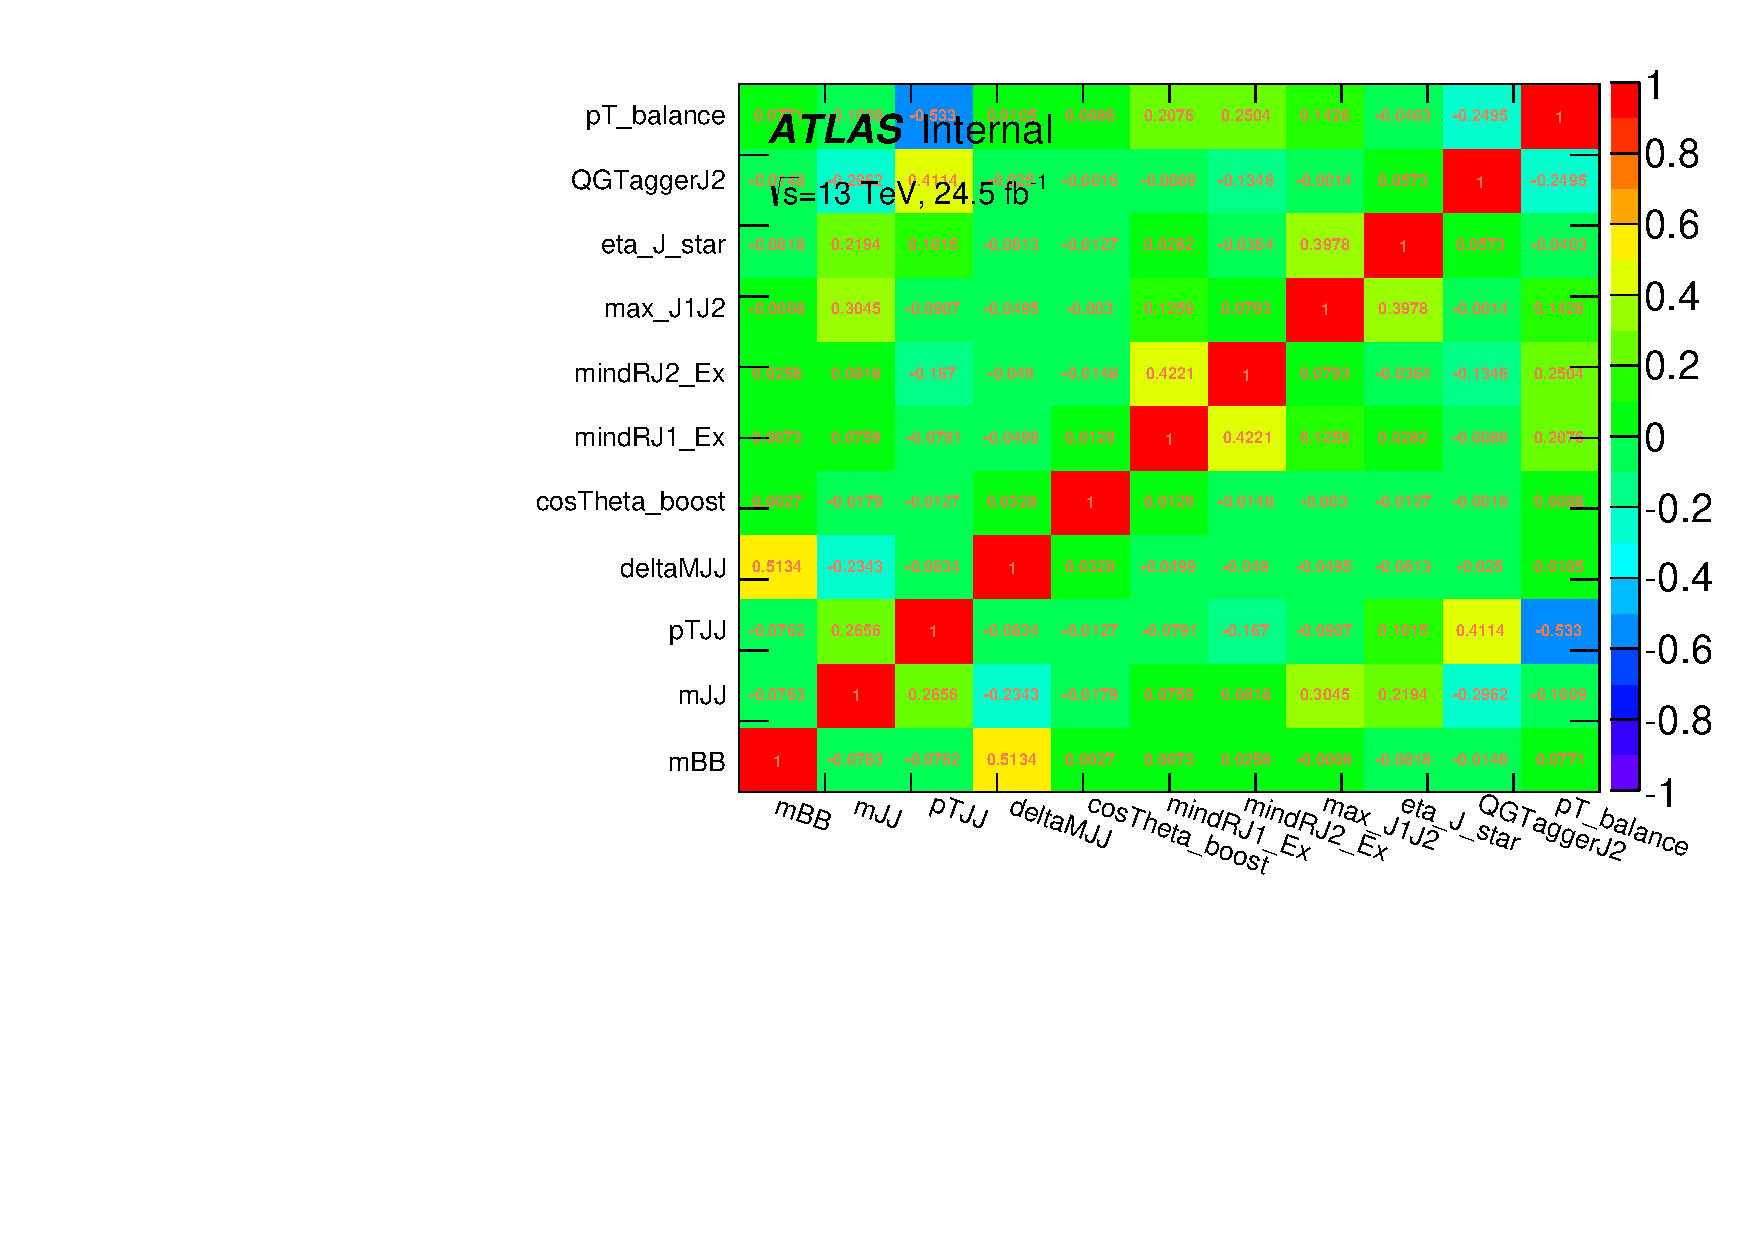
\includegraphics[width=0.48\textwidth]{figures/VBF/BDT_VBF_var_cor_2cen.pdf}
 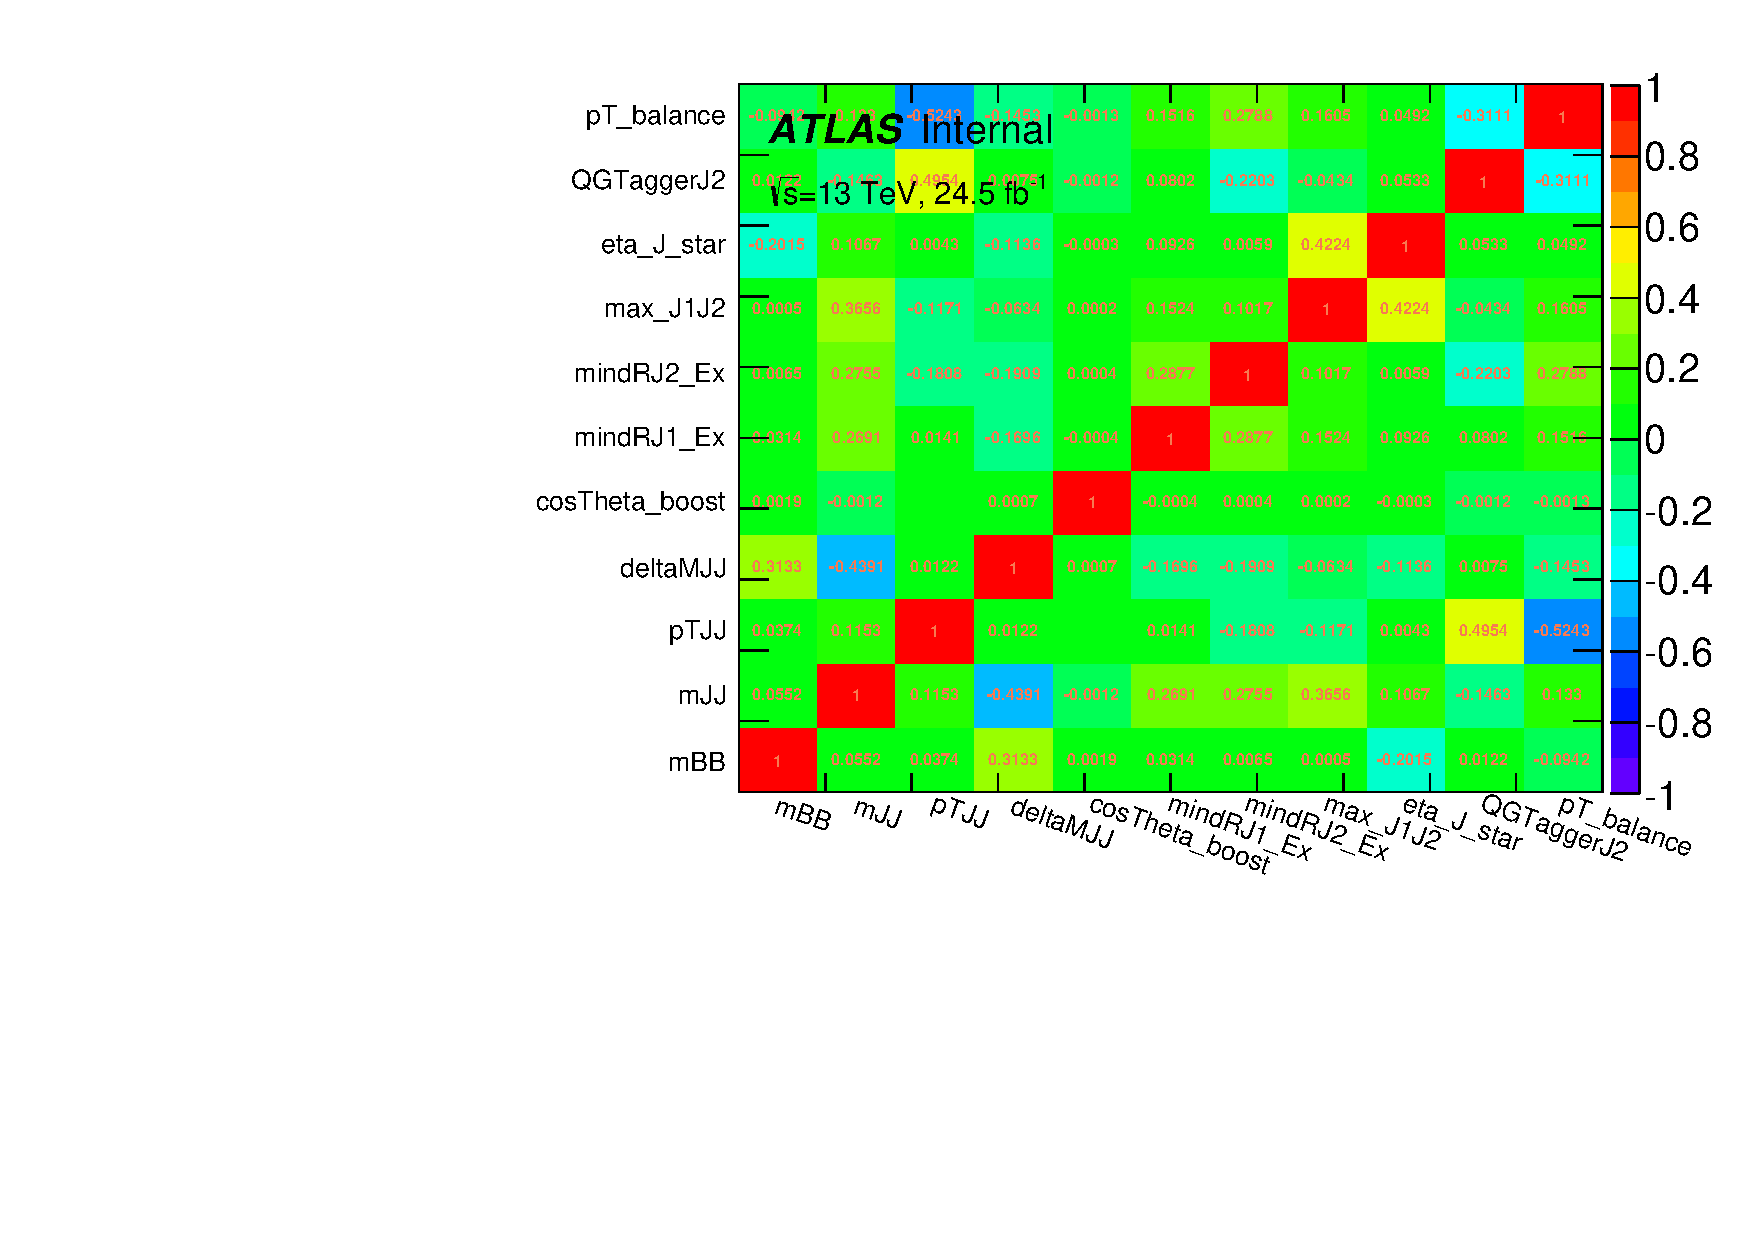
\includegraphics[width=0.48\textwidth]{figures/VBF/BDT_data_var_cor_2cen.pdf}\\
 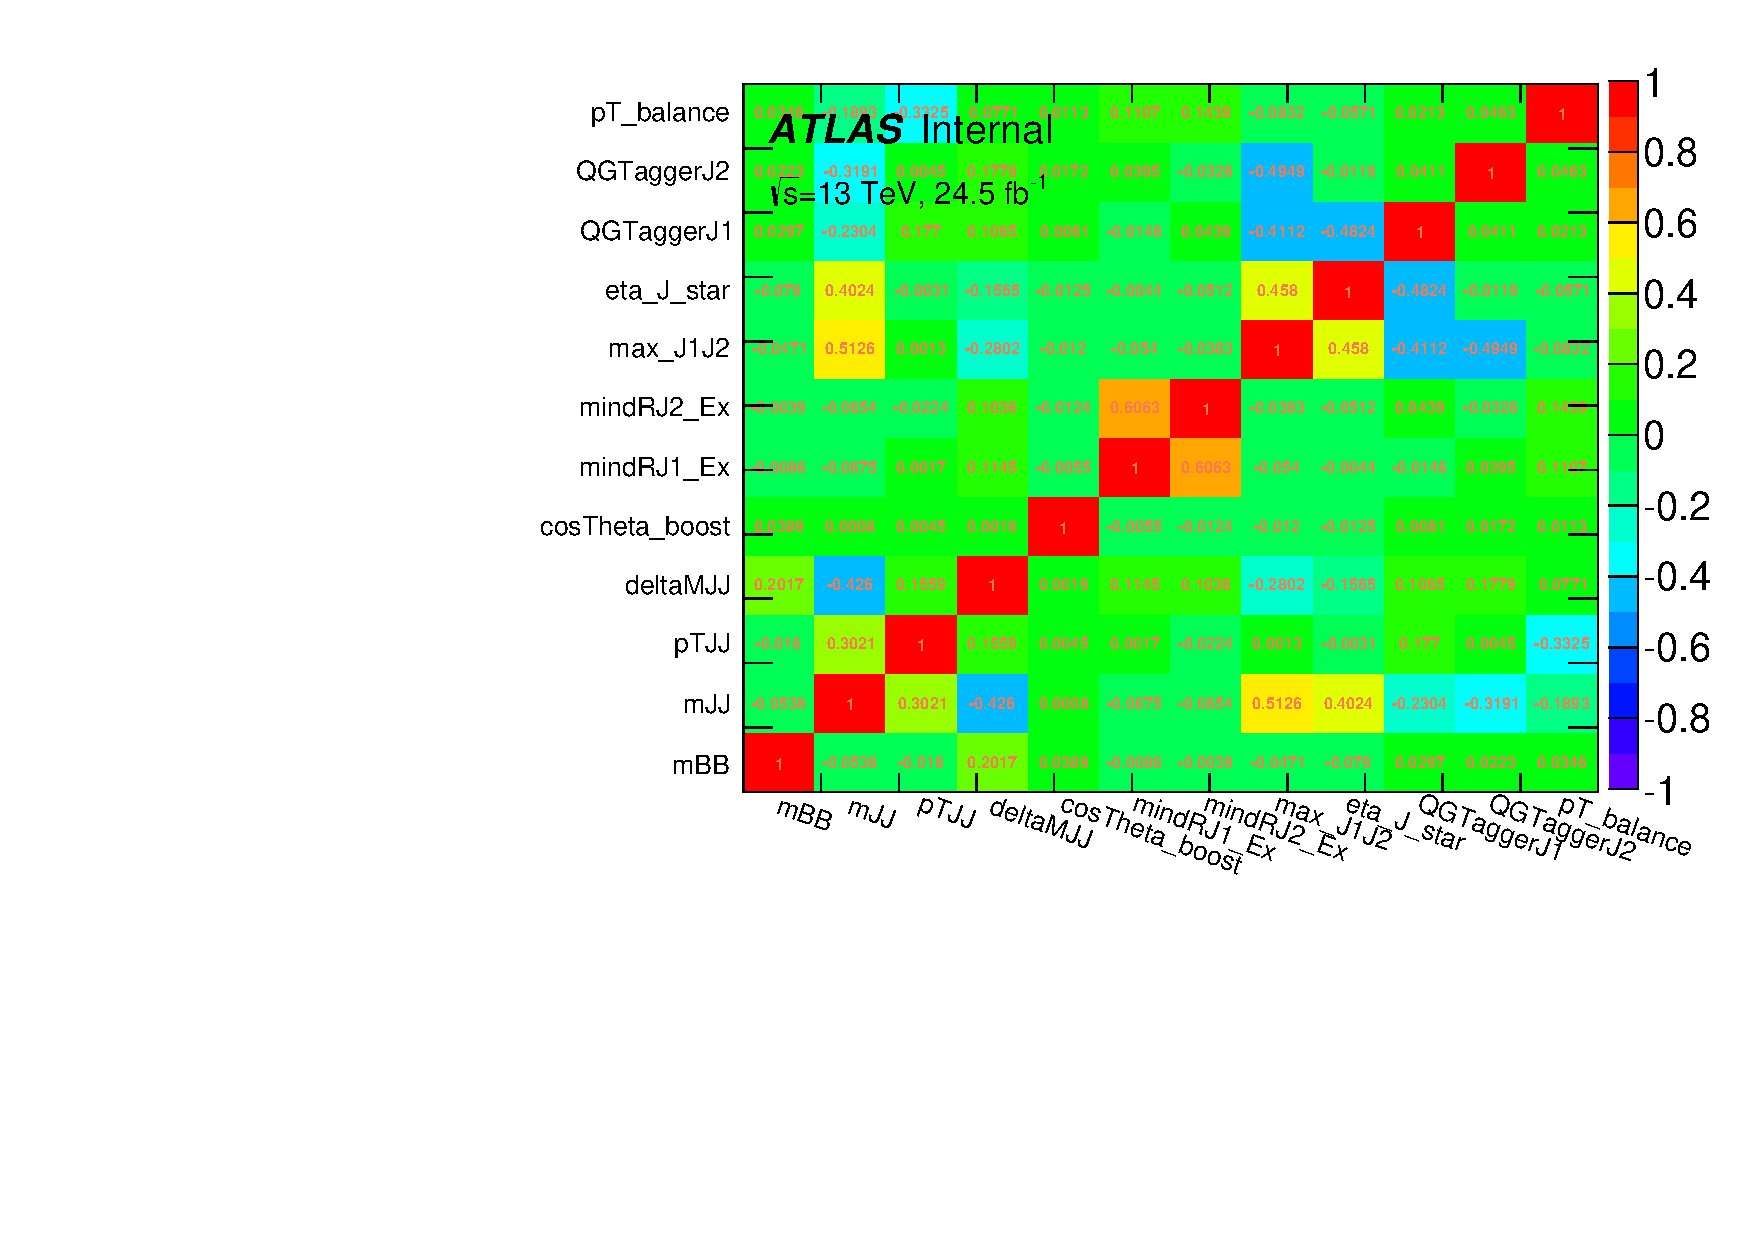
\includegraphics[width=0.48\textwidth]{figures/VBF/BDT_VBF_var_cor_4cen.pdf}
 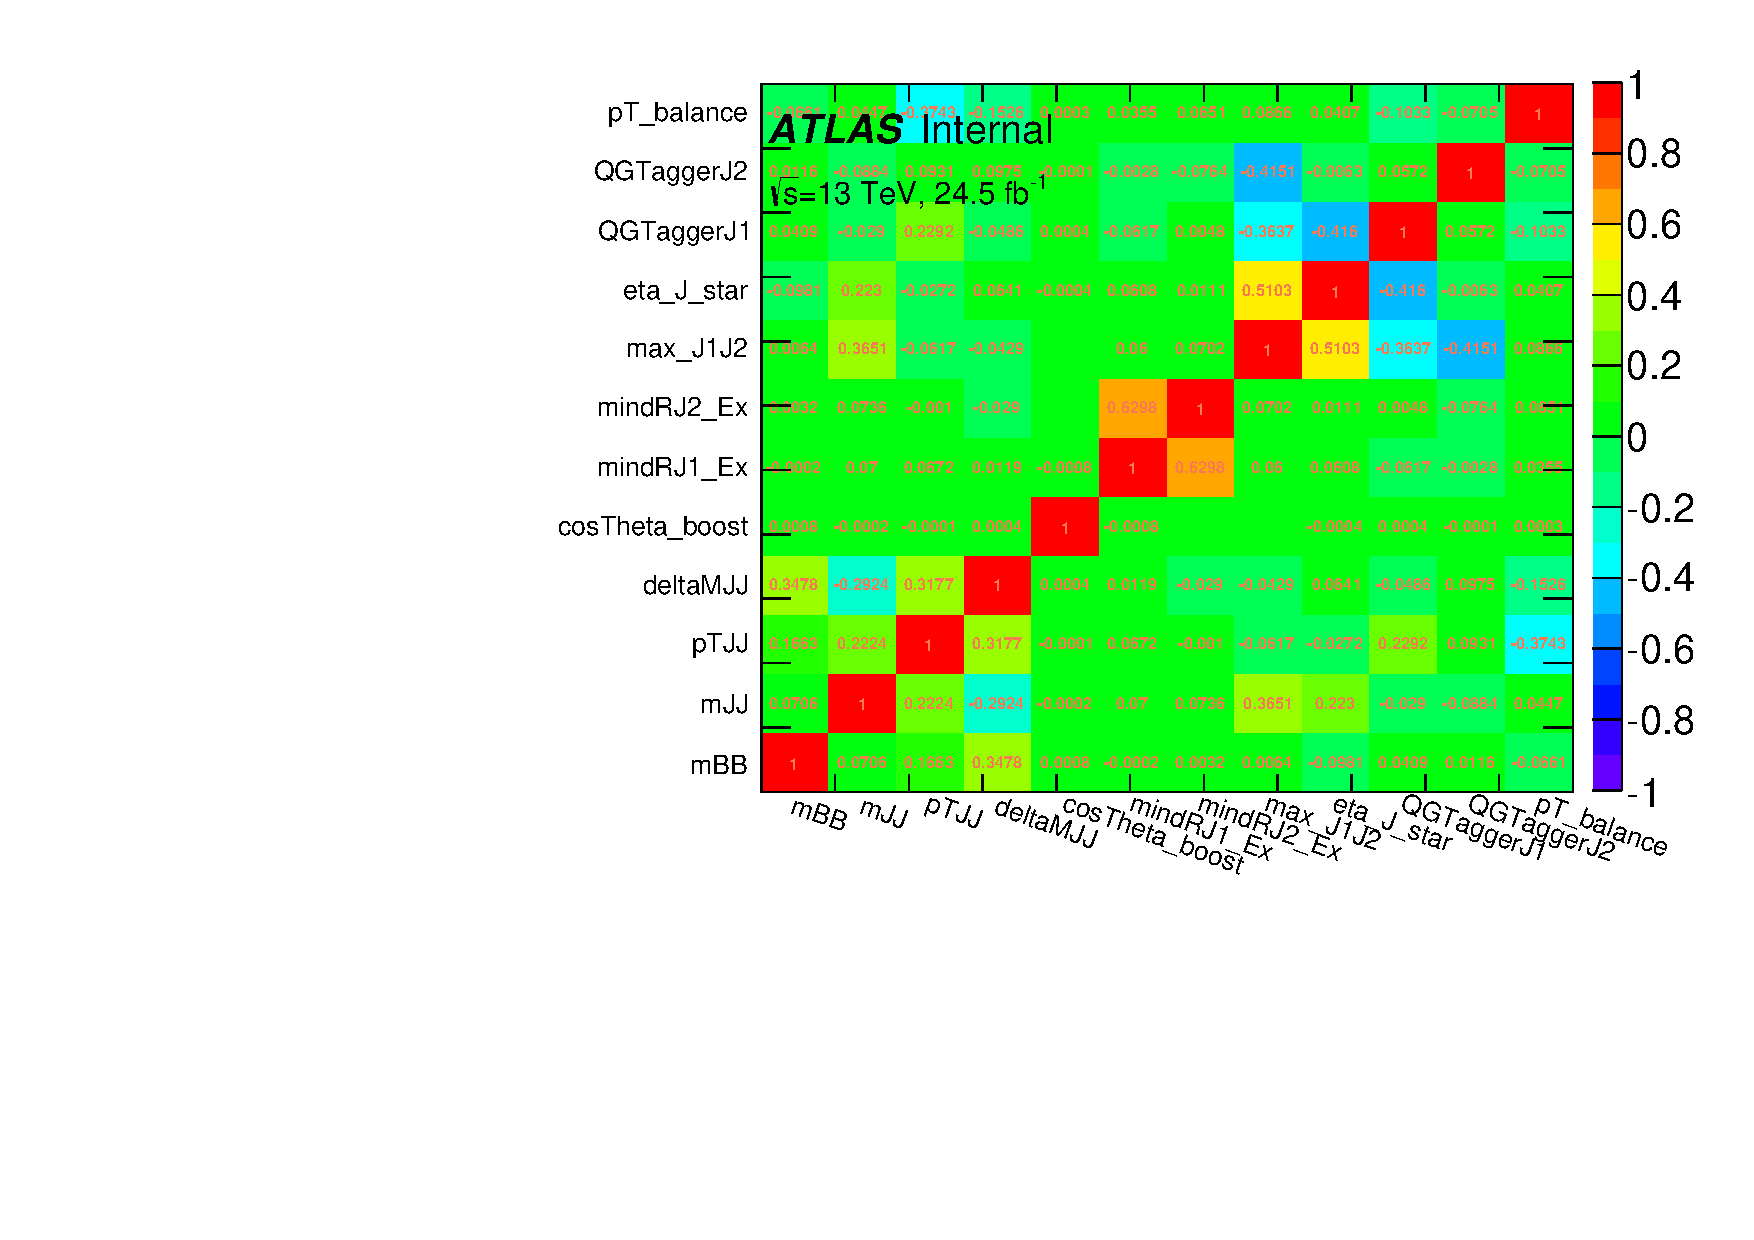
\includegraphics[width=0.48\textwidth]{figures/VBF/BDT_data_var_cor_4cen.pdf}\\
\caption{Correlations between BDT input variables and $\Mbb$ of signal (left) and background (right) of  the \twocentral (top) and \fourcentral (bottom) channels.}
  \label{fig:vbf-BDTInputsCor}
\end{figure}


\begin{figure}[htbp]
  \centering
 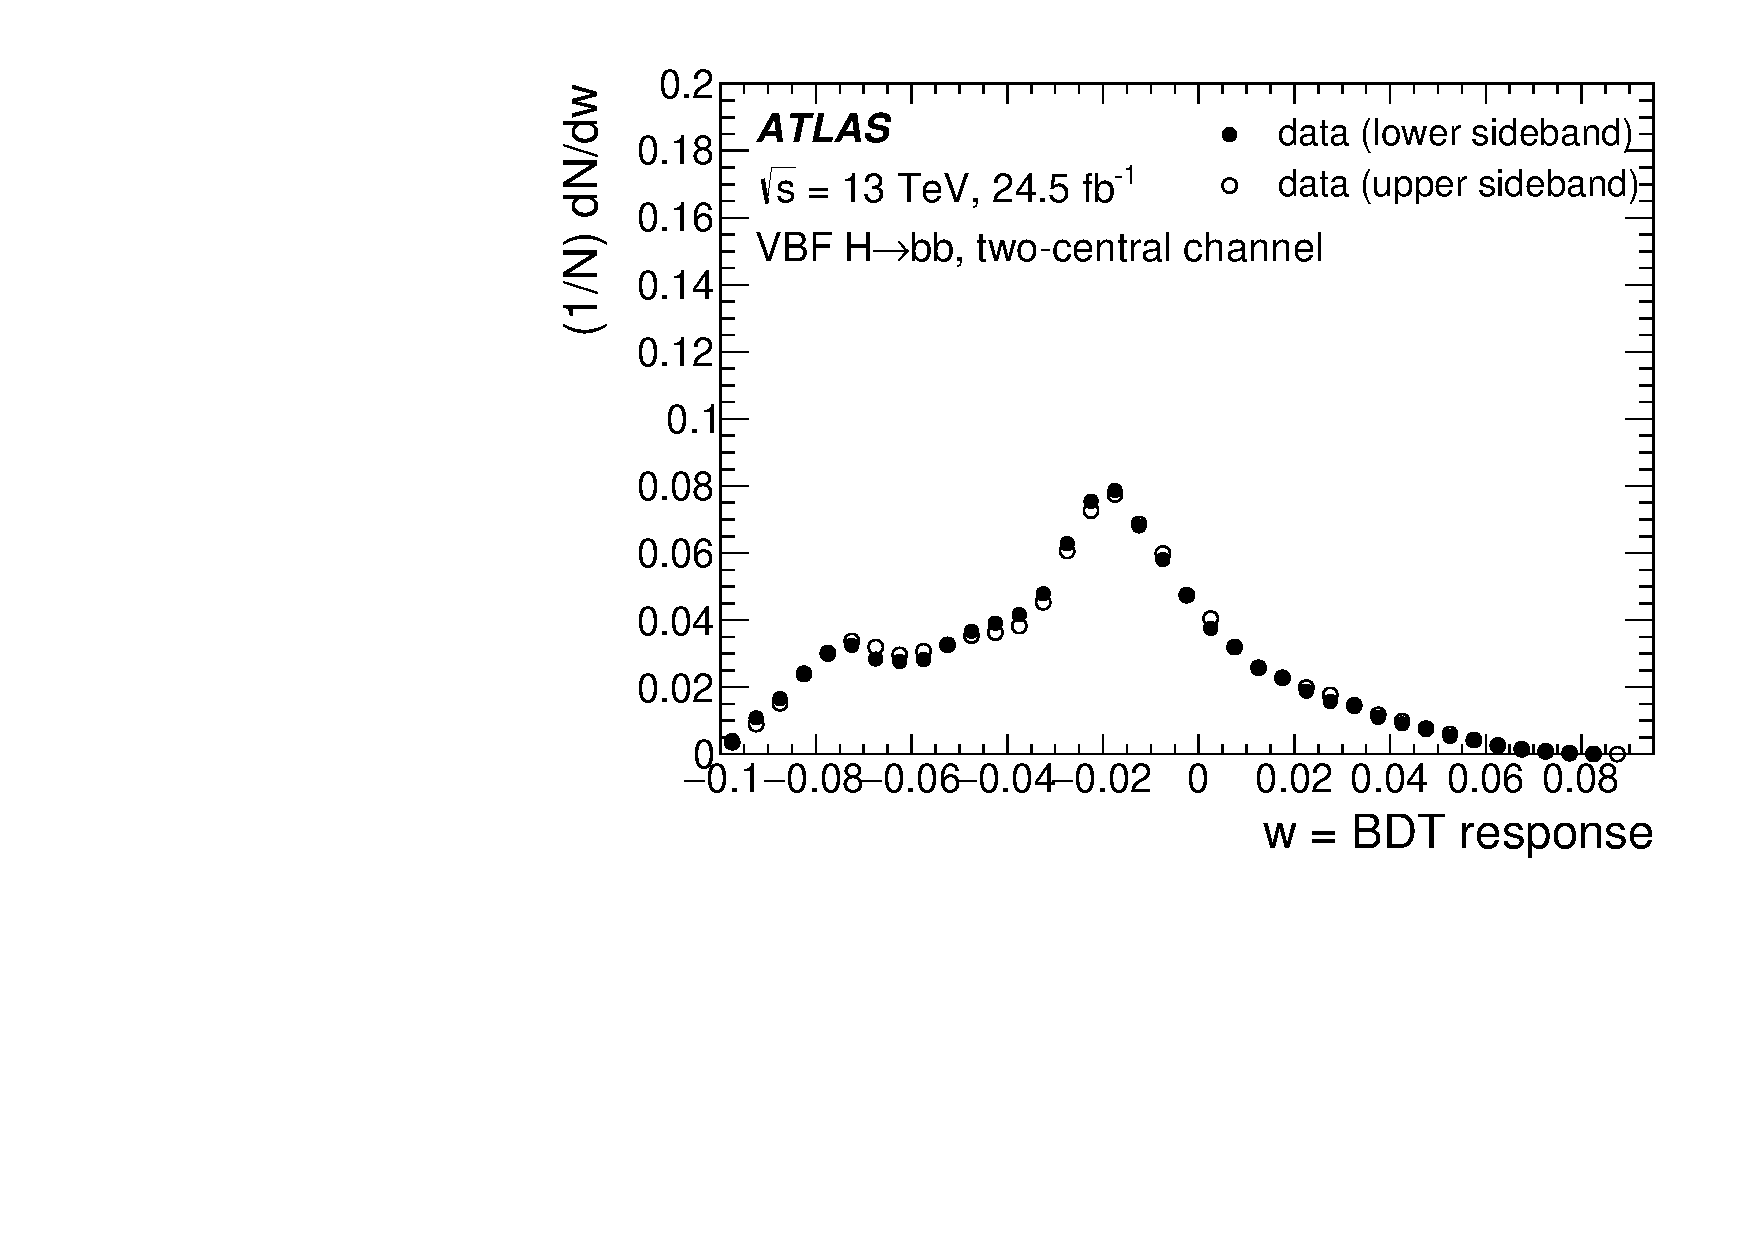
\includegraphics[width=0.48\textwidth]{figures/VBF/VBF_BDT_sidebands_2cen.pdf}
 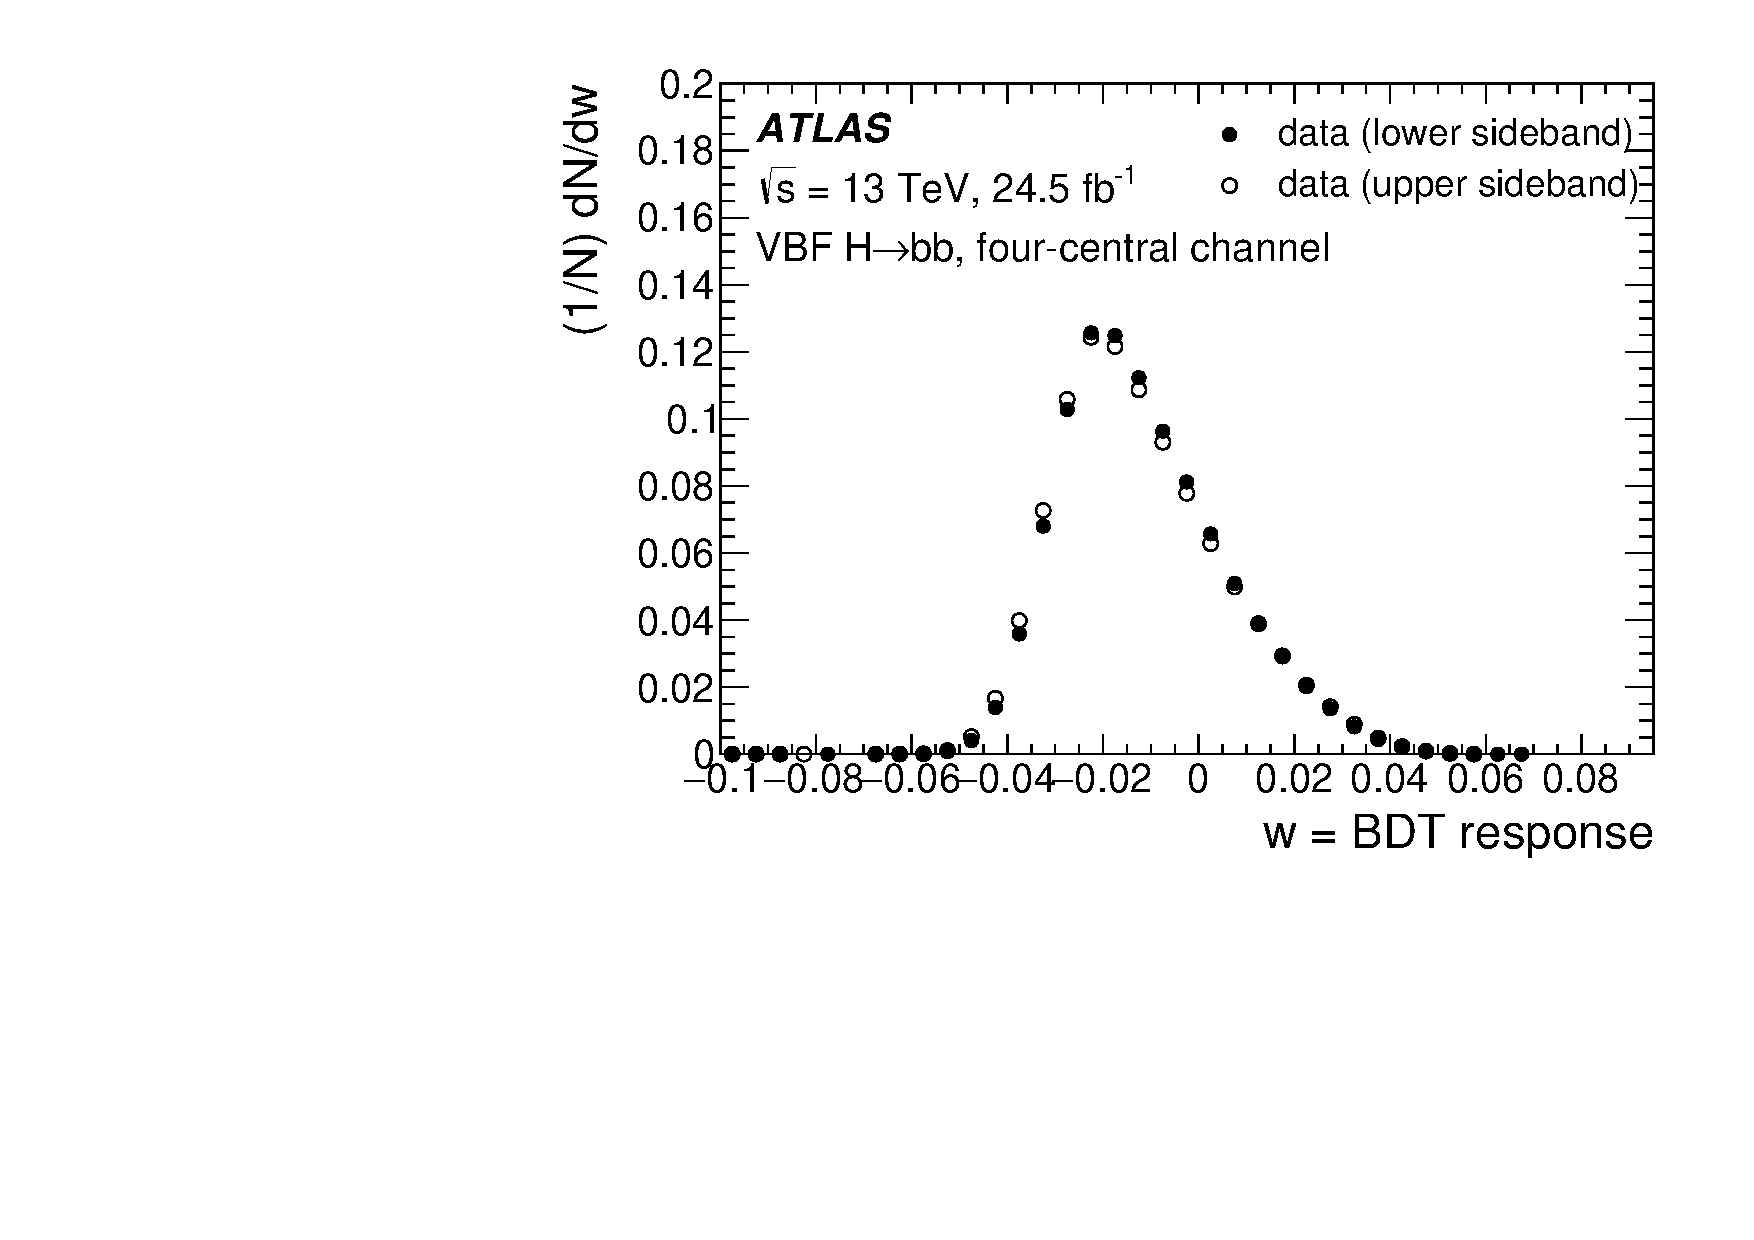
\includegraphics[width=0.48\textwidth]{figures/VBF/VBF_BDT_sidebands_4cen.pdf}
\caption{Comparison of the BDT response distributions between lower and upper data sideband events for the \twocentral (left) and \fourcentral channels. No obvious BDT response dependence on \Mbb is observed. }
  \label{fig:vbf-bdtsidebands}
\end{figure}




%The most correlated variables with \Mbb is $\Delta M_{\rm JJ}$.
%Further studies of the correlation with \Mbb and the BDT variables,
%the relative importance of each variable in the BDT, and a 3-fold
%validation test are shown in Appendix~\ref{sec:vbf-app-bdt}.
%From these studies we conclude that the BDT discriminant is not
%significantly correlated with \Mbb with the exception of very high BDT scores.

The BDT response for  the signal and background training and validation
samples for both channels is shown in Figure~\ref{fig:vbf-BDTResponse}.
In the \fourcentral channel the VBF \Hbb BDT distribution peaks at 0.03.
The background sample peaks at -0.02.  In the \twocentral channel the
VBF \Hbb distribution has a single broad peak at 0.05 and the
background peaks at -0.02. Good agreement is seen between the training
and validation datasets, indicating that the BDT training is adequate.
A Kolmogorov-Smirnov test is used to check the compatibility between
the training and validation datasets.  The \twocentral channel has
a 0.52 $p$-value for the observed agreement in the background sample
and 0.58 $p$-value for the signal sample. The \fourcentral channel has
a $p$-value of 0.95 for the background and $p$-value of 0.99 for the signal.
Figure~\ref{fig:vbf-BDTResponse} also shows the compatibility of the BDT
shapes for all samples considered in this analysis.
The ggF Higgs production and QCD-produced \zjets ~ samples have a
nearly identical response to the background sample in the \fourcentral channel.
In the \twocentral channel these samples have a slightly higher average BDT score than the background distribution.
The EWK \zjets ~ production has a most probable BDT score which is higher than the
background samples, but less than the VBF \Hbb sample in both cases.



\begin{figure}[htbp]
  \centering
 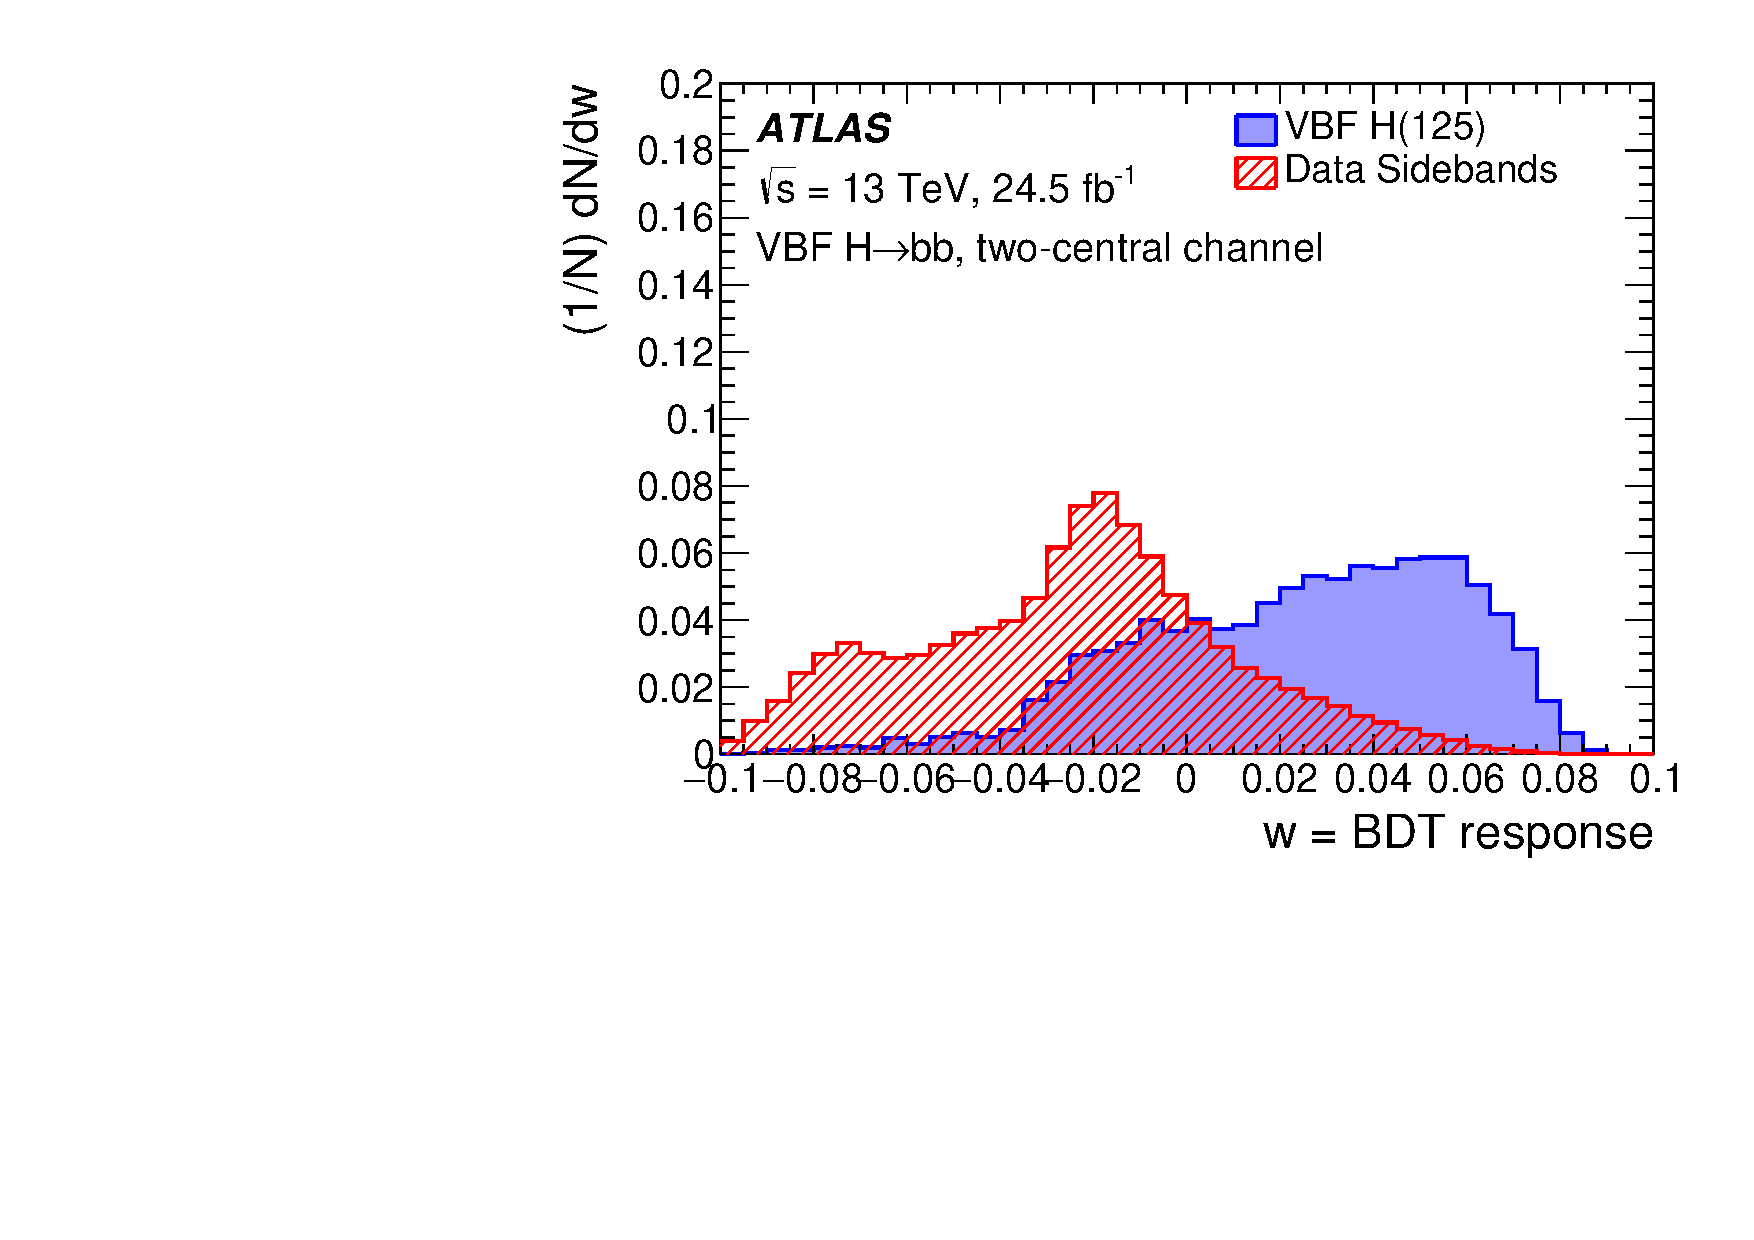
\includegraphics[width=0.48\textwidth]{figures/VBF/BDT_response_2cen.pdf}
 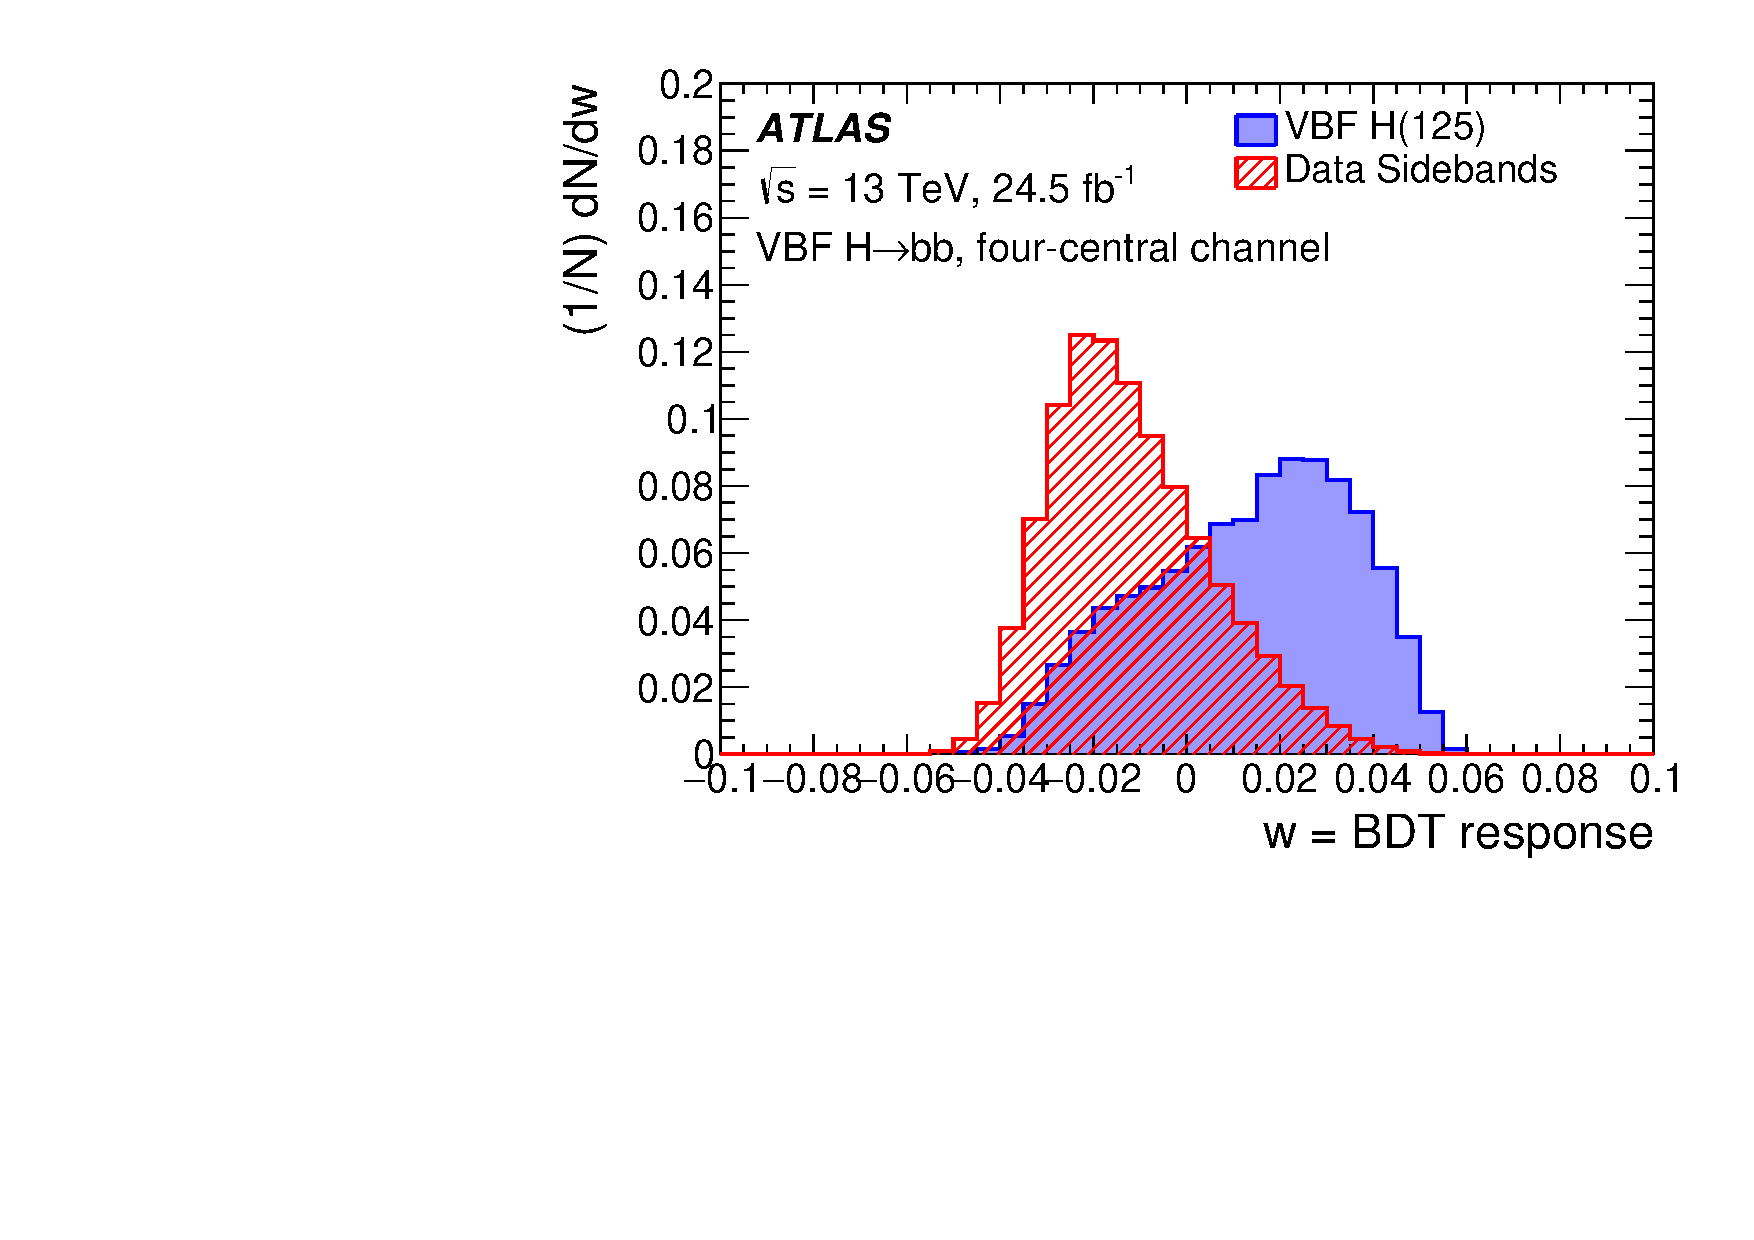
\includegraphics[width=0.48\textwidth]{figures/VBF/BDT_response_4cen.pdf}\\
 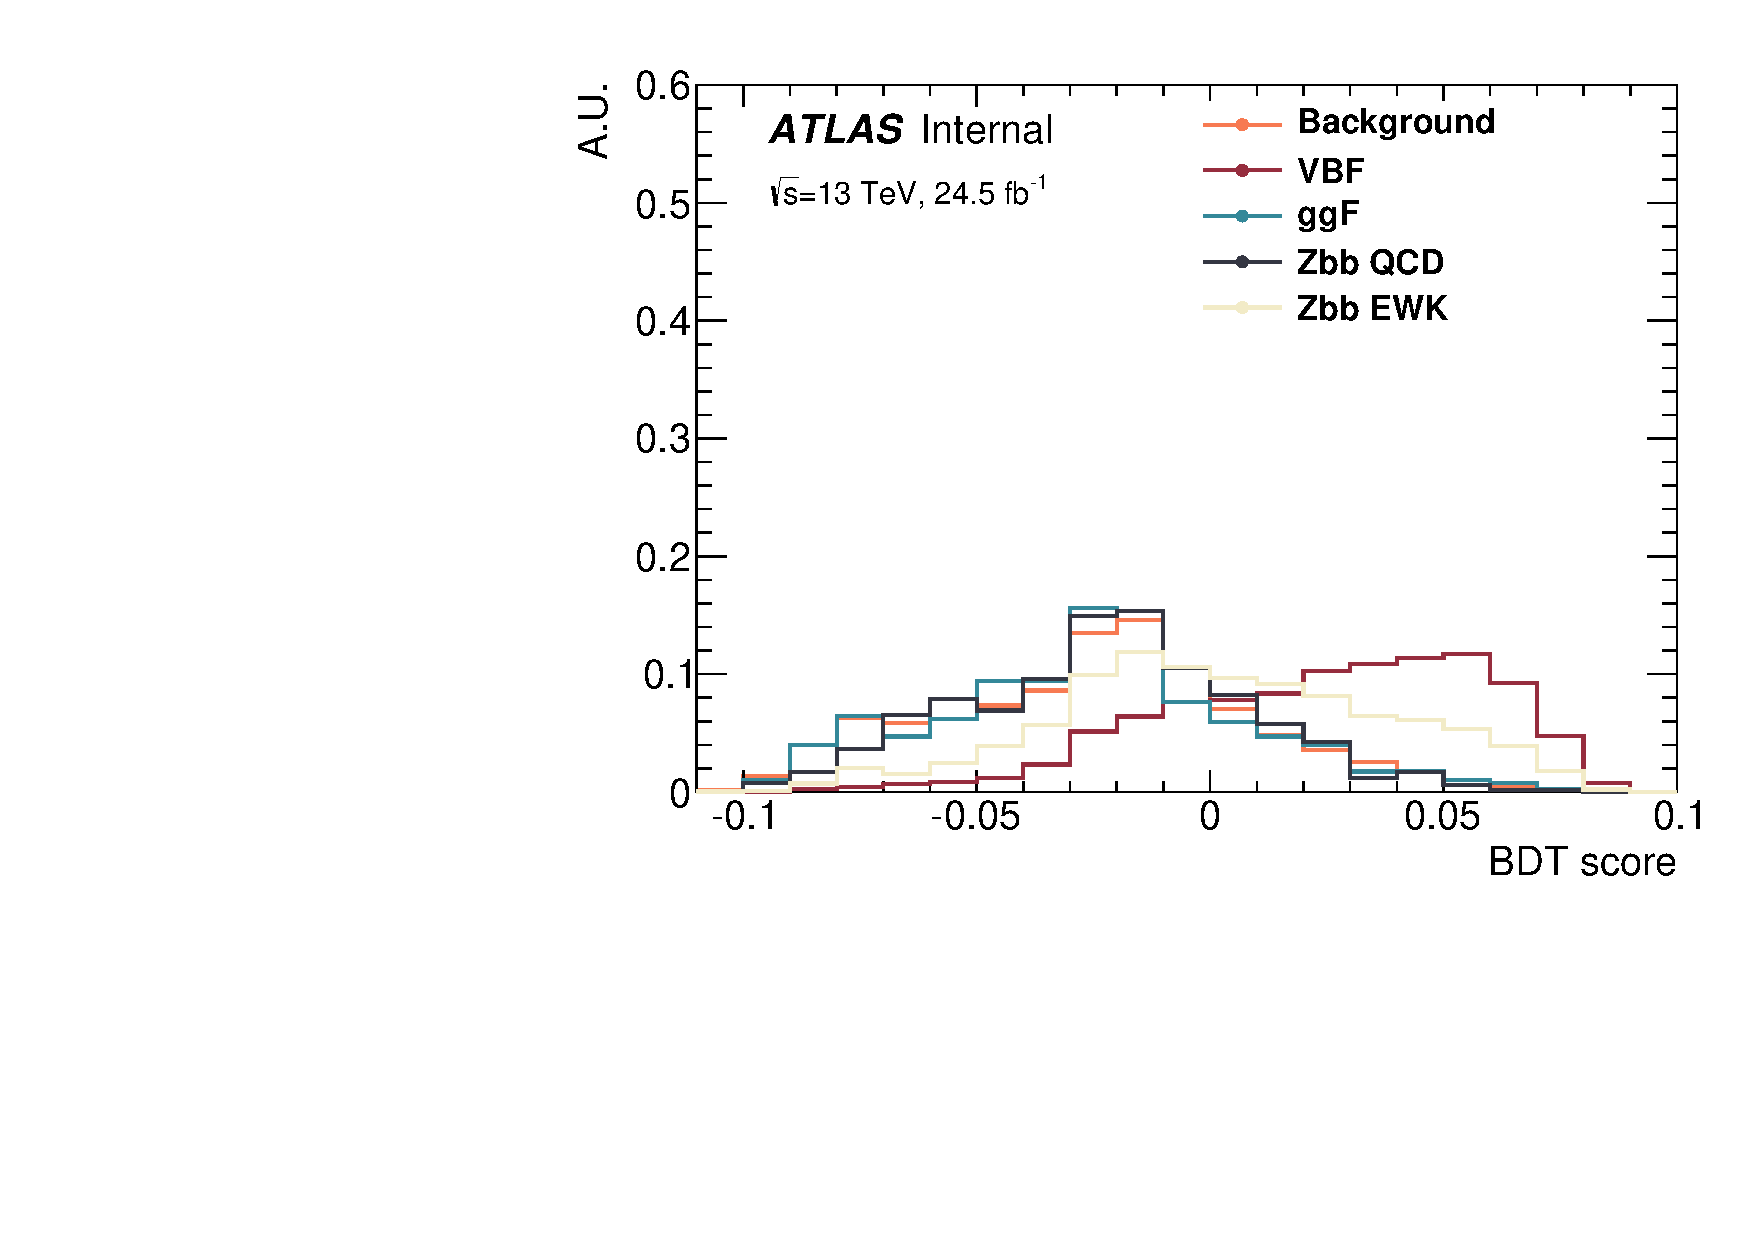
\includegraphics[width=0.48\textwidth]{figures/VBF/BDT_score_breakdown_2cen.pdf}
 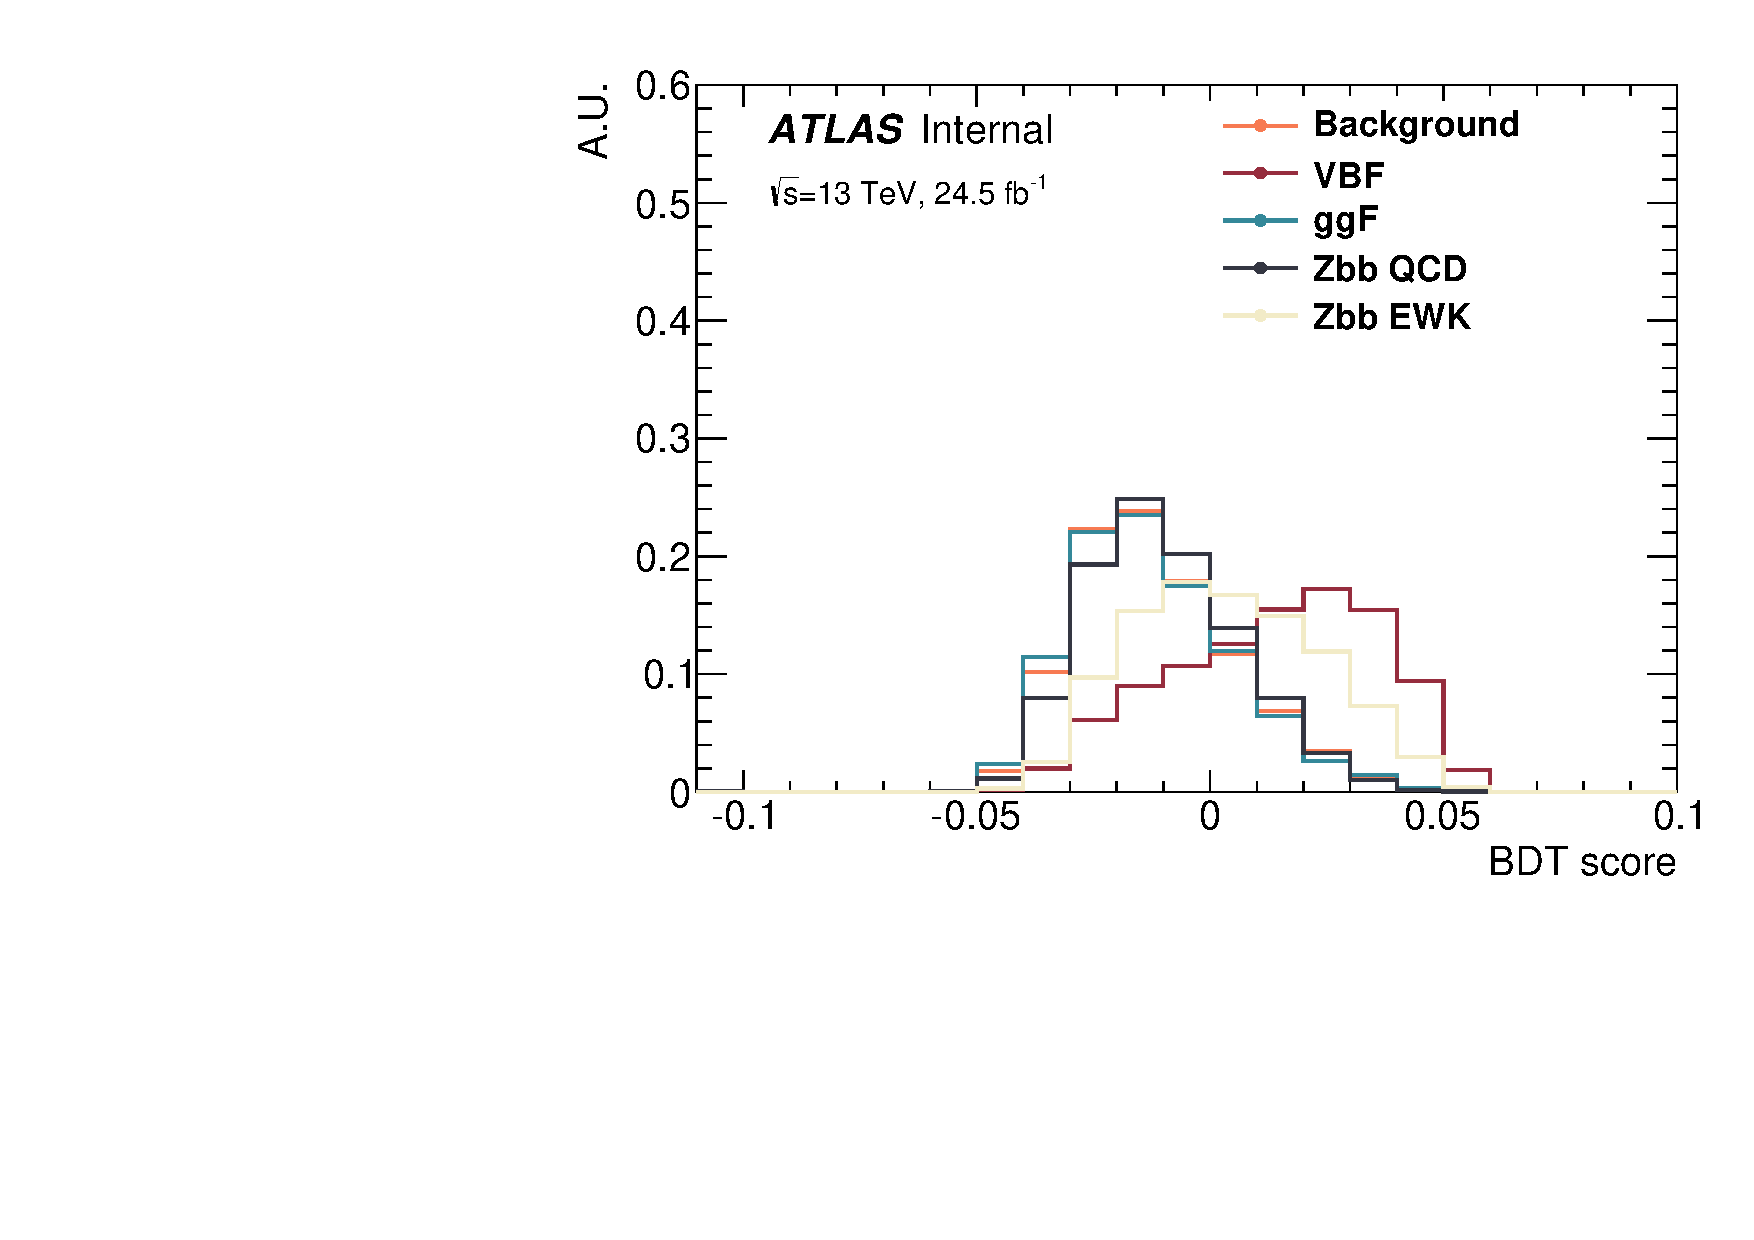
\includegraphics[width=0.48\textwidth]{figures/VBF/BDT_score_breakdown_4cen.pdf}\\
\caption{BDT Response for  the \twocentral (left) and \fourcentral (right) channel.  The top row shows the response for both the training and validation samples.  The bottom row shows a comparison of response for the signal, multijet background, $ggF$ Higgs and $Z$ boson samples. }
  \label{fig:vbf-BDTResponse}
\end{figure}


\subsection{Signal Regions}
For the \twocentral channel, we choose a region in which
a sufficiently large number of \zjets{} events pass the BDT to
adequately control the contribution of this background in the final fit.
The top 80\% of the VBF signal events pass this requirement to define the first signal region.
The second encompasses the remainder of the BDT distribution. This definition of the regions
is a conservative approach that ensures a constraining power of the \zjets{} contribution
sufficient to prevent biasing the Higgs strength as the leading order $Z$ MC
modeling might not be accurate and we have to float its contribution in the fit.

%(see Section~\ref{sec:vbf-ztreat} and Appendix~\ref{sec:vbf-app-alternative2cen} for more details). 
%Alternative definitions of the SRs, aimed at maximizing the sensitivity for the Higgs boson, 
%have been considered and discarded in favor of having higher precision in determining the \zjets{} contribution in each region.
%Table~\ref{tab:BDTSensitivity} illustrates the impact of the choice of SR I definition on the overall Higgs sensitivity and 
%the precision on the \zjets{} contribution in that region.
%For example, extending the lower boundary of the SR I from including 50\% to 80\% VBF events, 
%the \zjets{} contribution grows by a factor of five, corresponding to a 2.7 times improvement in constraining power, while the Higgs sensitivity is reduced by 17\%.   The last column of Table~\ref{tab:BD%TSensitivity} is chosen as the BDT region definition. 

For the \fourcentral channel, we scan the VBF signal events in the entire BDT scores to maximize the sum of $\frac{S}{\sqrt{B}}$ for the top 70\% VBF signal to define in total four signal regions. In this channel, the \zjets{} contribution is larger and the constraining power in each SR is adequate to prevent large bias to the Higgs strength (see Section~\ref{sec:vbf-zunblind}).
Therefore the manual adjustment of the SR boundaries adopted for \twocentral is not necessary.

The definition of the signal regions, the yields of each processes and the estimation of sensitivity are listed in Tables~\ref{tab:BDTReg2cen_alt} and ~\ref{tab:BDTReg4cen_alt}. 


%\begin{table}[]
%\centering
%\caption{Higgs and \zjets{} sensitivity for different definitions of BDT regions in \twocentral channel. The $\Delta \mu_H$ is estimated with Asimov fit for all regions and channels combined. The $\Delta \mu_Z$ is estimated in sideband only fit for SR I of the \twocentral channel. The most sensitive region is always defined to retian VBF events with top x\% BDT scores. The rest of the regions are defined to maximize the sum of $\frac{S}{\sqrt{B}}$. The final configuration we choose is the last column such that we have sufficient constraining power of \zjets{}.}
%\label{tab:BDTSensitivity}
%\resizebox{\textwidth}{!}{
%\begin{tabular}{|c|c|c|c|c|c|}
%\hline
%                                                                                             & \begin{tabular}[c]{@{}c@{}}4 regions\\     SR I top 30\% VBF\end{tabular} & \begin{tabular}[c]{@{}c@{}}3 regions\\   SR I top 50\% VBF\end{tabular} & \begin{tabular}[c]{@{}c@{}}3 regions\\   SR I top 60\% VBF\end{tabular} & \begin{tabular}[c]{@{}c@{}}3 regions\\   SR I top 70\% VBF\end{tabular} & \begin{tabular}[c]{@{}c@{}}2 regions\\   SR I top 80\% VBF\end{tabular} \\ \hline
%$\Delta \mu_H$                                                                               & 1.4                                                                       & 1.67                                                                    & 1.71                                                                    & 1.78                                                                    & 1.84                                                                    \\ \hline
%\begin{tabular}[c]{@{}c@{}}$\Delta \mu_Z$\\ 2 central SR I\\ Sideband only fit\end{tabular}  & 5.0                                                                       & 3.37                                                                    & 2.6                                                                     & 1.6                                                                     & 1.25                                                                    \\ \hline
%\begin{tabular}[c]{@{}c@{}}\# Z events in \\ the side band of \\ 2 central SR I\end{tabular} & 51.19                                                                     & 140.8                                                                   & 214.5                                                                   & 445.3                                                                   & 760.34                                                                  \\ \hline
%\begin{tabular}[c]{@{}c@{}}\# Z events in\\  the sideband of \\ the rest of SRs\end{tabular} & 2263.7                                                                    & 2574.1                                                                  & 2500.4                                                                  & 2269.6                                                                  & 1954.56                                                                 \\ \hline
%\end{tabular}}
%\end{table}


\begin{table}[htpb]
\centering
\begin{tabular}{|l|l|l|}
\hline
Region                       & SR I                  & SR II                 \\ \hline
BDT Score Range              & \textgreater -0.006    & \textless -0.006       \\ \hline
\multicolumn{3}{|c|}{Total Yield}                                            \\ \hline
QCD $Z$                      & $946.2 \pm 91.1$    & $2525.3 \pm 145.9$  \\ \hline
EWK $Z$                      & $70.9 \pm 2.3$      & $54.6 \pm 2.1$      \\ \hline
\multicolumn{3}{|c|}{Sideband}                                               \\ \hline
Non-resonant (sideband low)  & $22812 \pm 151.0$    & $62742 \pm 250.5 $   \\ \hline
Non-resonant (sideband high) & $38020 \pm 195.2$    & $100936 \pm 317.7 $  \\ \hline
\multicolumn{3}{|c|}{Yield in Higgs Mass Window}                             \\ \hline
VBF                          & $101.2 \pm 2.0$     & $22.2\pm 0.9$       \\ \hline
ggF                          & $23.7 \pm 2.6$      & $75.8\pm 6.1$       \\ \hline
Non-resonant (extrapolated)   & $32546.0 \pm 180.4$ & $92738.2 \pm 304.5$ \\ \hline
\multicolumn{3}{|c|}{Expected Sensitivity}                                   \\ \hline
$S/ \sqrt(B)$                & 0.70                  & 0.32                  \\ \hline
\end{tabular}
\caption{Signal region definitions, yields and sensitivities for the \twocentral channel. }
\label{tab:BDTReg2cen_alt}

\end{table}


\begin{table}[htpb]
\centering
\begin{tabular}{|l|l|l|l|l|}
\hline
Region                       & SR I                & SR II                      & SR III                     & SR IV                      \\ \hline
BDT Score Range              & \textgreater0.033   & [0.026, 0.033]             & [0.015, 0.026]             & [0.002, 0.015]             \\ \hline
\multicolumn{5}{|c|}{Total Yield}                                                                                                         \\ \hline
QCD $Z$                      & $64.1 \pm 14.8$   & $787.8 \pm 66.2$         & $2485.9 \pm 132.1$       & $7274.4 \pm 206.1$       \\ \cline{2-5} 
EWK $Z$                      & $12.3 \pm 0.8$    & $63.5 \pm 1.7$           & $128.2 \pm 2.4$          & $184.0 \pm 2.9$          \\ \hline
\multicolumn{5}{|c|}{Sideband}                                                                                                            \\ \hline
Non-res. (sideband low)  & $8626 \pm 92.9$    & $13998 \pm 118.3 $        & $43393 \pm 208.3$         & $108343 \pm 329.2$        \\ \cline{2-5} 
Non-res. (sideband high) & $12267 \pm 110.8$  & $18550 \pm 136.2$         & $55413 \pm 235.4$         & $134435 \pm 366.7$        \\ \hline
\multicolumn{5}{|c|}{Yield in Higgs Mass Window}                                                                                          \\ \hline
VBF                          & $51.6 \pm 0.6$    & $28.4\pm 0.3$            & $43.1\pm 0.5$            & $41.9\pm 0.5$            \\ \cline{2-5} 
ggF                          & $11.3 \pm 0.4$    & $13.2 \pm 0.4$           & $43.4 \pm 1.4$           & $127.0 \pm 1.5$          \\ \cline{2-5} 
Non-res. (extrapolated)   & $8797.1 \pm 93.8$ & $15685.8\pm 125.2$       & $53156.7\pm 230.6$       & $142273.1\pm 377.2$      \\ \hline
\multicolumn{5}{|c|}{Expected Sensitivity}                                                                                                \\ \hline
$S/ \sqrt(B)$                & 0.67                & 0.33                       & 0.38                       & 0.45                       \\ \hline
\end{tabular}
\caption{Signal region definitions, yields and sensitivities for the \fourcentral channel. }
\label{tab:BDTReg4cen_alt}

\end{table}




\clearpage

\subsection{Fit  Strategy and Background Determination}
\label{sec:fitbkgds}
\label{sec:vbf-nonres}

In order to determine the non-resonant background, we fit  the sidebands of each of the BDT regions independently with an analytical function. The sidebands of the \Mbb{}  distribution of each BDT region are shown in Fig. \ref{fig:vbf-mbb_sidebands}. %An alternative approach  using a control region and a linear transfer factor to relate the control region shape to the signal regions is documented in Appendix~\ref{sec:vbf-app-oldfitbkgds}.  However, due to concerns about the validity of the approach, documented in Appendix~\ref{sec:vbf-app-LinearityTest}, the more conservative approach of independent fits is taken here.  

\begin{figure}[htbp]
  \centering
 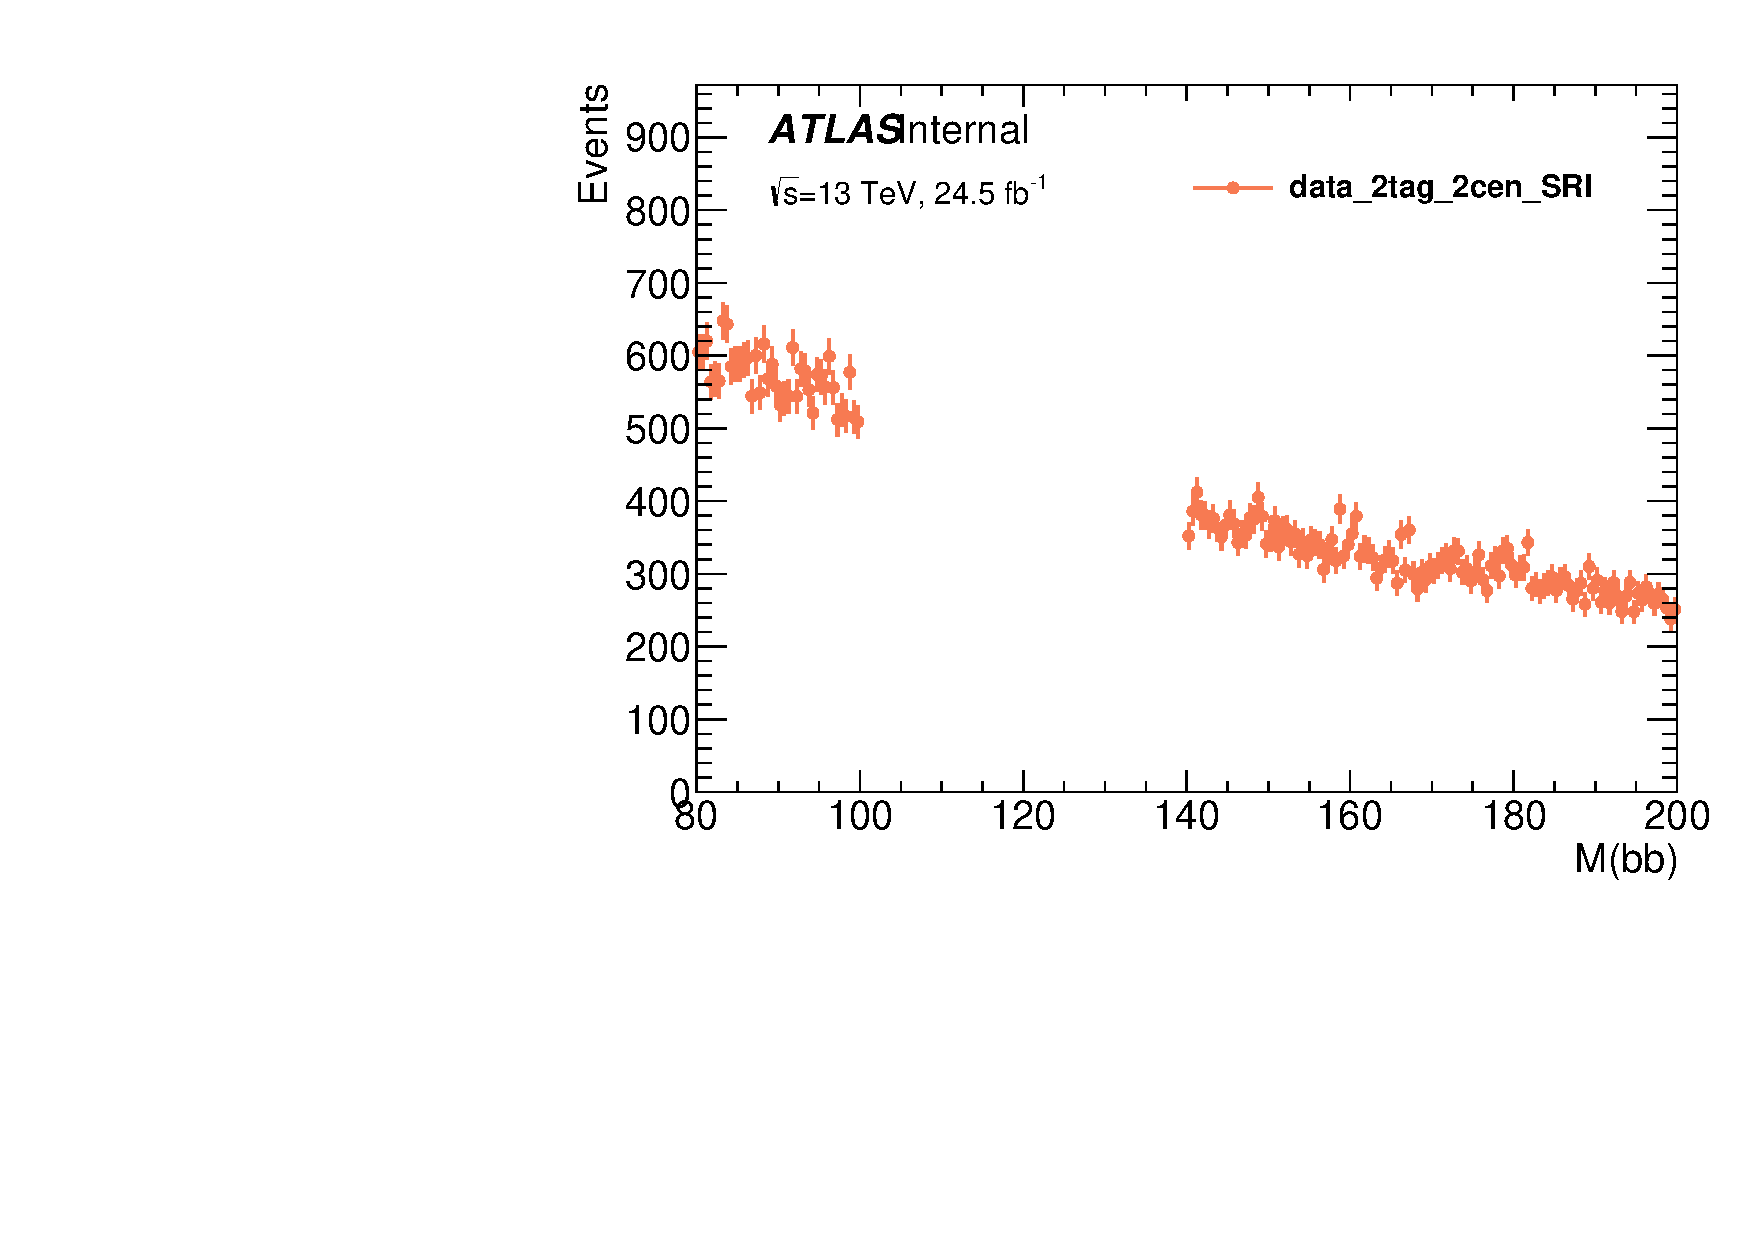
\includegraphics[width=0.45\textwidth]{figures/VBF/Mbb_SRI_2cen.pdf}
 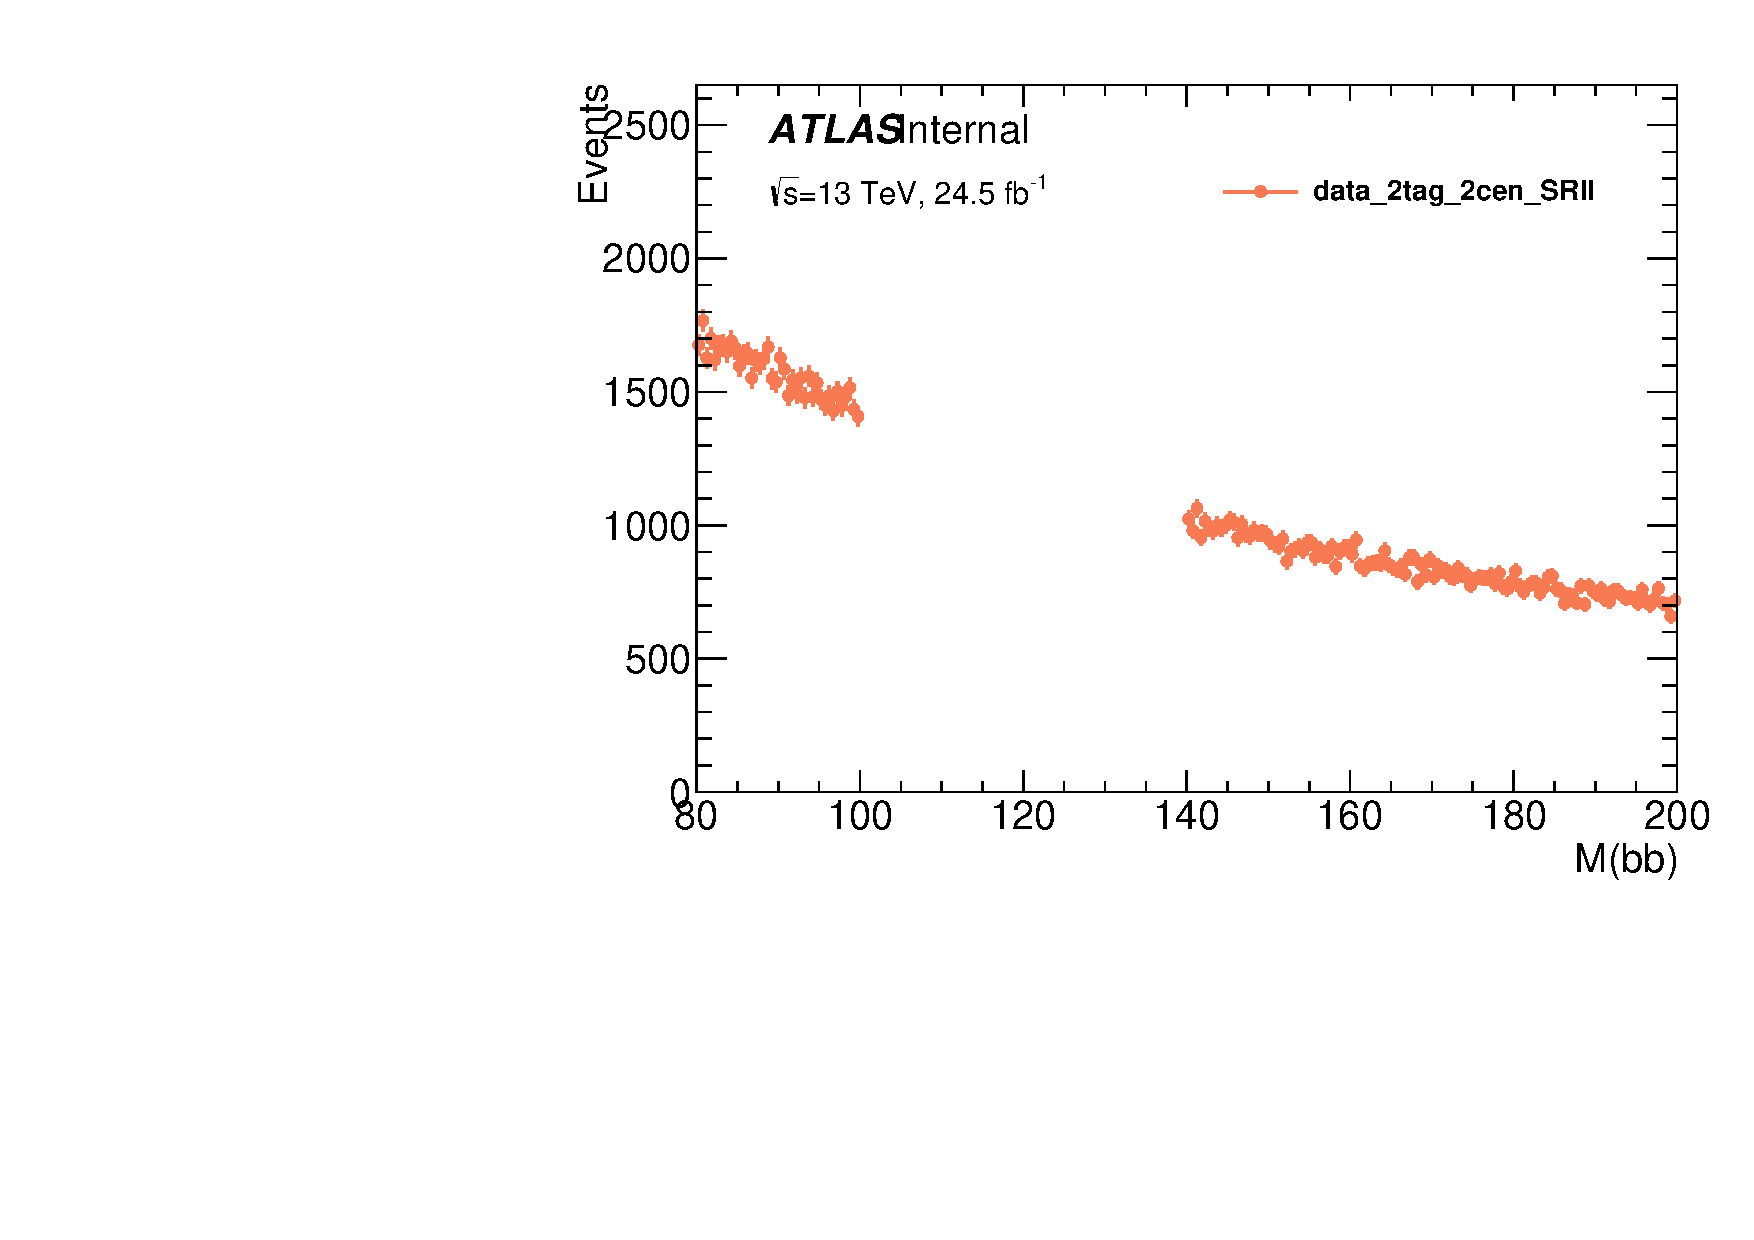
\includegraphics[width=0.45\textwidth]{figures/VBF/Mbb_SRII_2cen.pdf}\\
 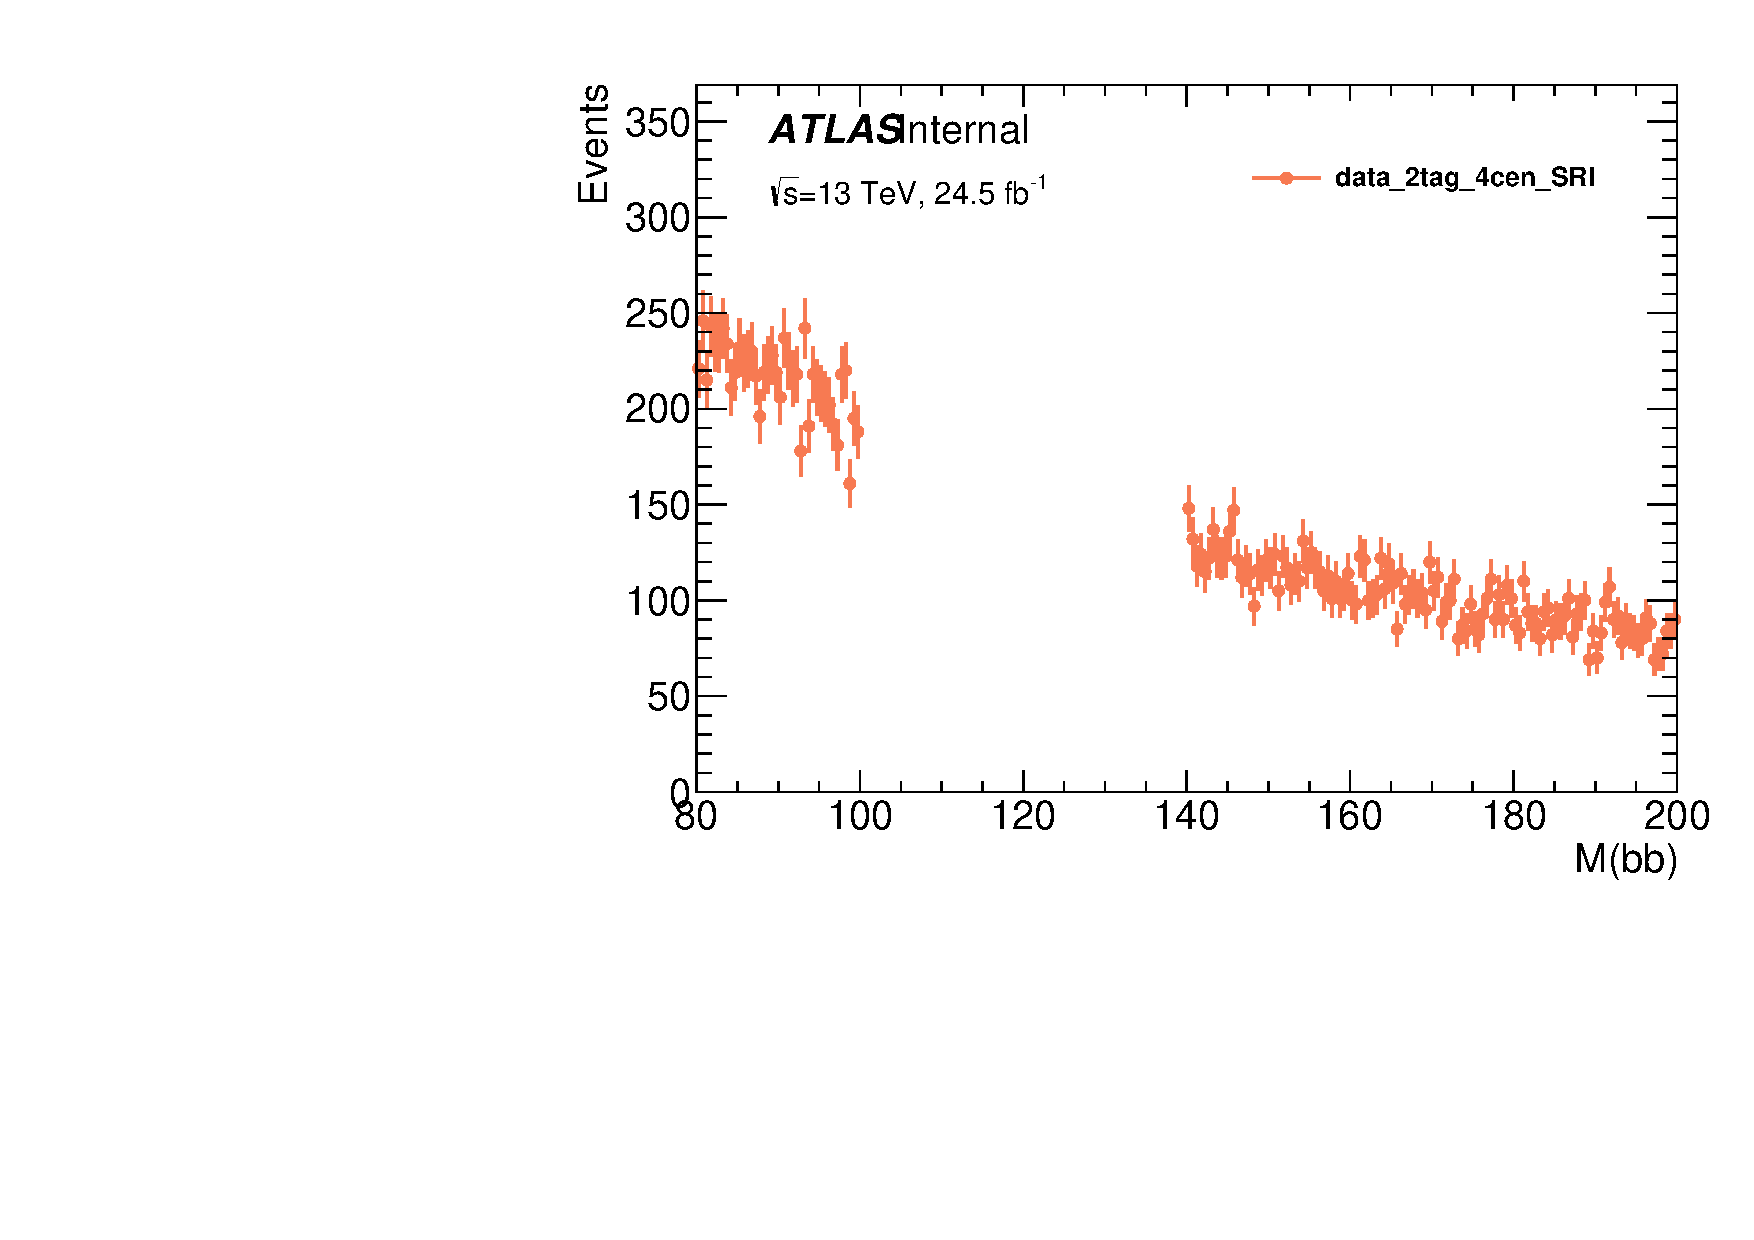
\includegraphics[width=0.45\textwidth]{figures/VBF/Mbb_SRI_4cen.pdf}
 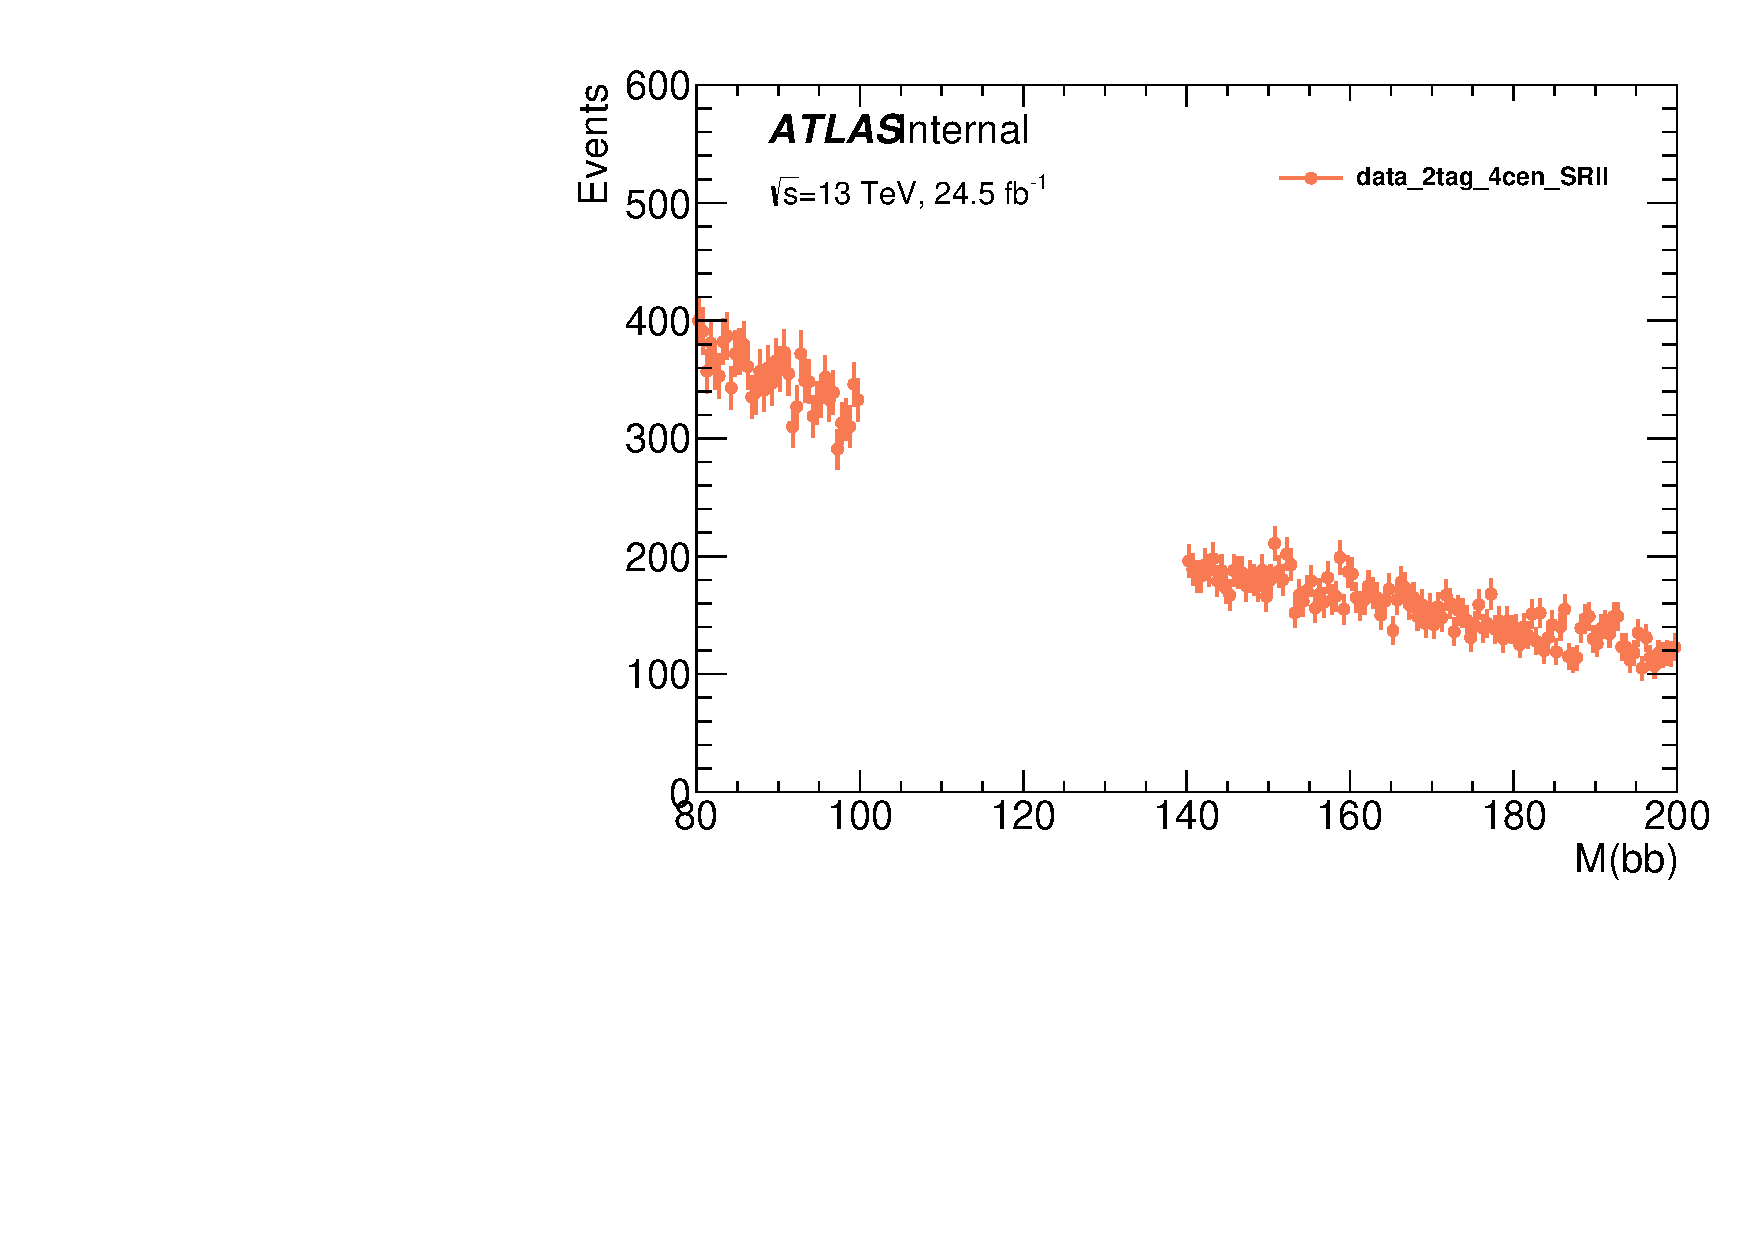
\includegraphics[width=0.45\textwidth]{figures/VBF/Mbb_SRII_4cen.pdf}\\
 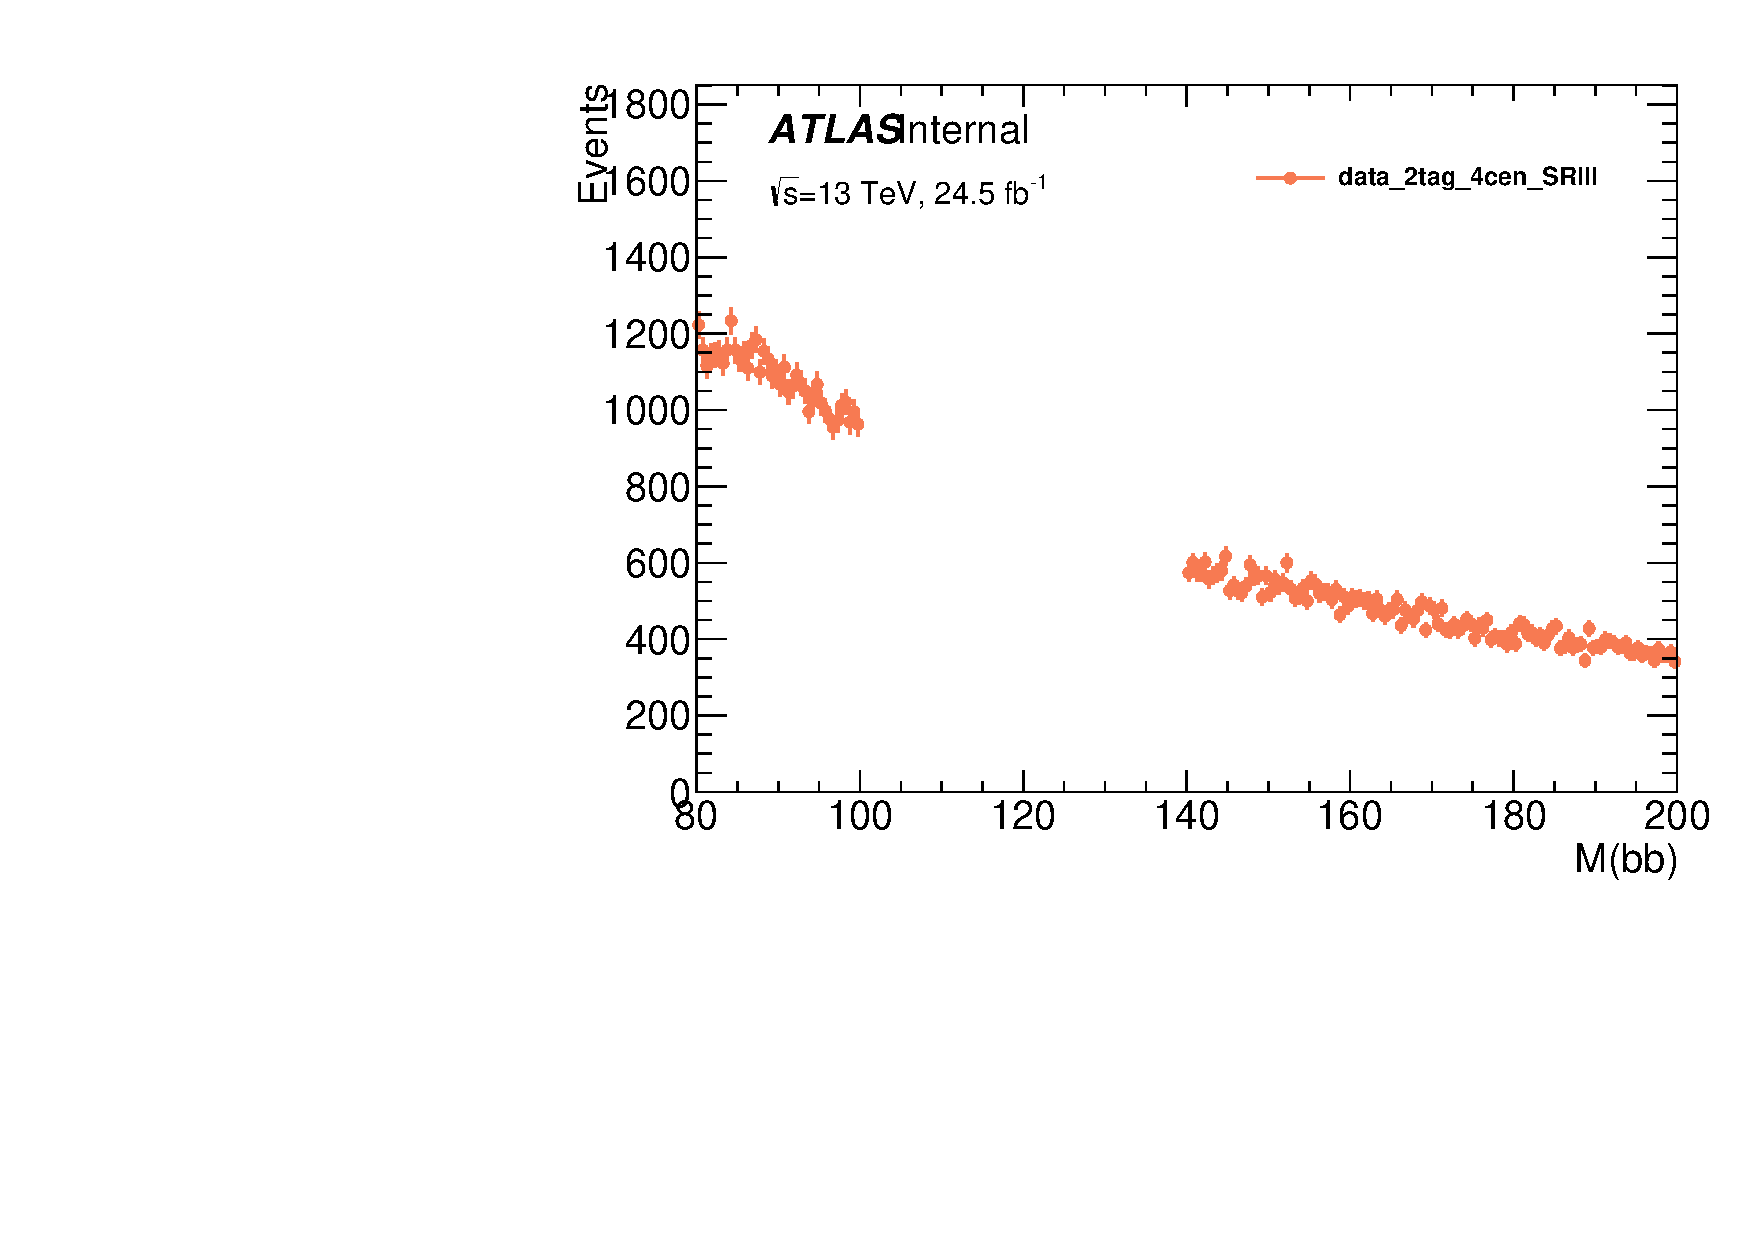
\includegraphics[width=0.45\textwidth]{figures/VBF/Mbb_SRIII_4cen.pdf}
 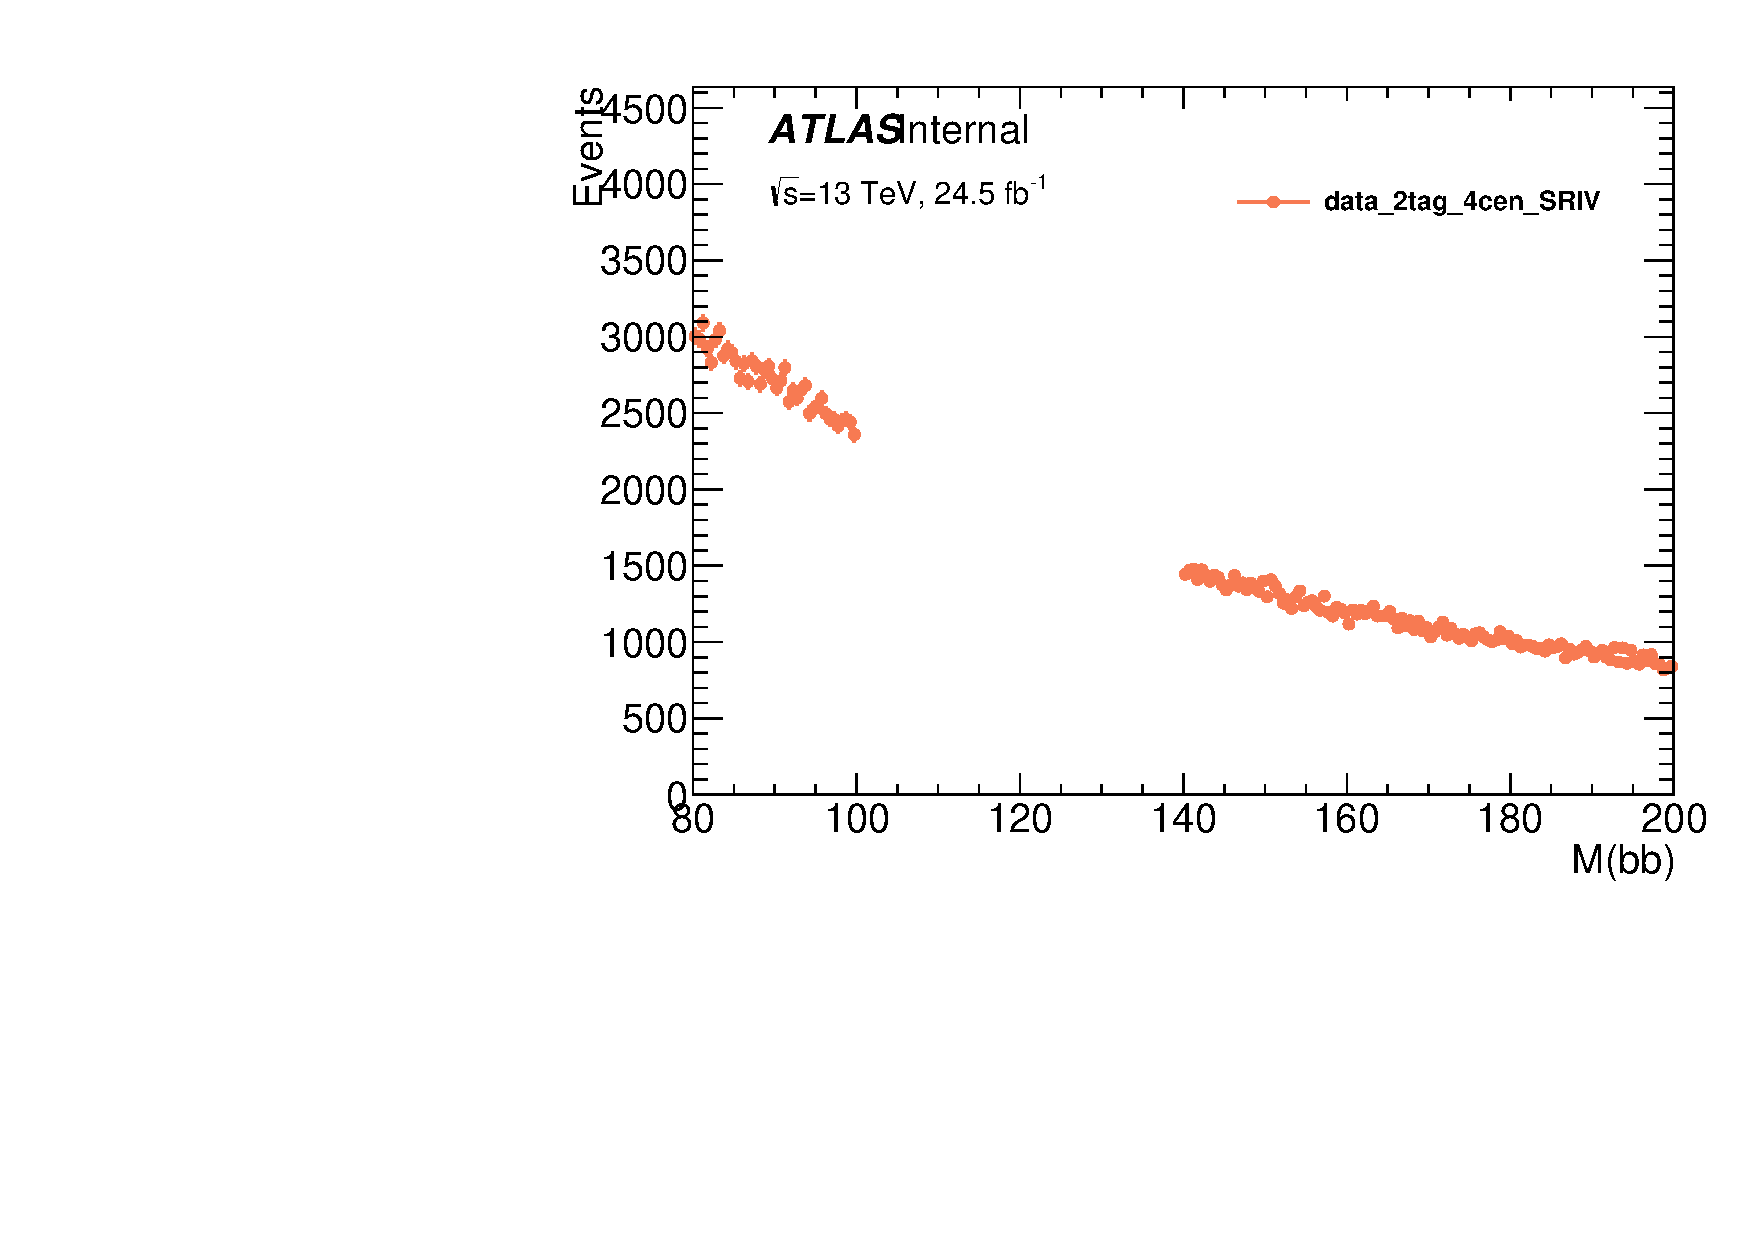
\includegraphics[width=0.45\textwidth]{figures/VBF/Mbb_SRIV_4cen.pdf}\\
\caption{\Mbb{} shapes of all BDT regions in sidebands} 
  \label{fig:vbf-mbb_sidebands}
\end{figure}


Several function families are considered and tested. The primary family of functions considered is that of the Bernstein polynomials listed in Equation~\ref{eq:bernstein}, which were
used successfully in the previous iteration of this analysis. The product of Bernstein and exponential functions, as well as the sum of exponentials, were used as the alternative functions for background description.
The functions chosen are required to pass two conditions. Among the candidates satisfying the conditions above, the function with the smallest number of degrees of freedom is chosen.

\begin{itemize}
\item 
Compatibility: The function must be statistically  compatible with the sidebands of the \Mbb{} distribution in the signal regions, where the Higgs mass range $100<\Mbb<140$ GeV is ignored. The compatibility criterion is defined as $P(\chi^2)>0.05$ and $P(F-\rm{test})>0.05$,  where the $\chi^2$ and $F-\rm{test}$ probabilities are considered, respectively. The $F-\rm{test}$ is performed with respect to the $n+1$ order function.  Only statistical errors are considered in these fits.  Among the candidates satisfying the conditions above, the function with the smallest number of degrees of freedom is chosen. For this study, the \zjets{} component is included in the fit,  normalized to the SM prediction.

\item Spurious Signal:  The lowest order function that satisfies compatibility condition, $f_{B}$, is tested against the the lowest order functions in an alternative truth model, $f_{A}$, that also satisfies the compatibility condition, to derive the spurious signal size \cite{CMS-HIG-12-028}. This is a standard approach used for similar analysis. Although in the future this approach needs better understanding if it double counts partial statistical uncertainty of data, we adopt this apporach to be conservative in estimating uncertainty. We build pseudo data from $f_{A}$, where the parameters of the function are derived from the fit to the sidebands in each signal region.  We then fit the distribution with $f_{B}$ plus $\mu_{sp}$ times the signal template. The measured  apparent signal size needs to be less than $50\%$ of the actual signal size. If this test fails, the the next order function satisfying the compatibility condition is tested.  The \zjets{} component is not included in the pseudo data.

\end{itemize}


The $\chi^2$ values and probabilities and $F-\rm{test}$ probabilities are summarized in Tables~\ref{tab:chi2-2cen} through~\ref{tab:f-test}. The $\chi^2$ test criteria are met for the O(2) Bernstein function in all regions, except in 
SR IV of the \fourcentral channel where we need at least an O(3) Bernstein function. The $F$-test is passed for functions which pass the $\chi^2$ criterion in all channels and regions.

The spurious signal fits are given in Tables~\ref{tab:spurious-test-2cen} and~\ref{tab:spurious-test-4cen}, which additionally show which functions are used as the alternative truth models. In most regions the O(3) Bernstein polynomial satisfies the spurious signal criterion. Note that our choice of background function minimizes the potential bias in trade of variance, i.e. the higher order functional forms yield larger uncertainty.

To satisfy all of the criteria, we choose an O(3) Bernstein function for the \twocentral channels, as well as for all SRs of the \fourcentral channel except SR IV which uses O(4).  


%\begin{figure}[htbp]
%  \centering
% 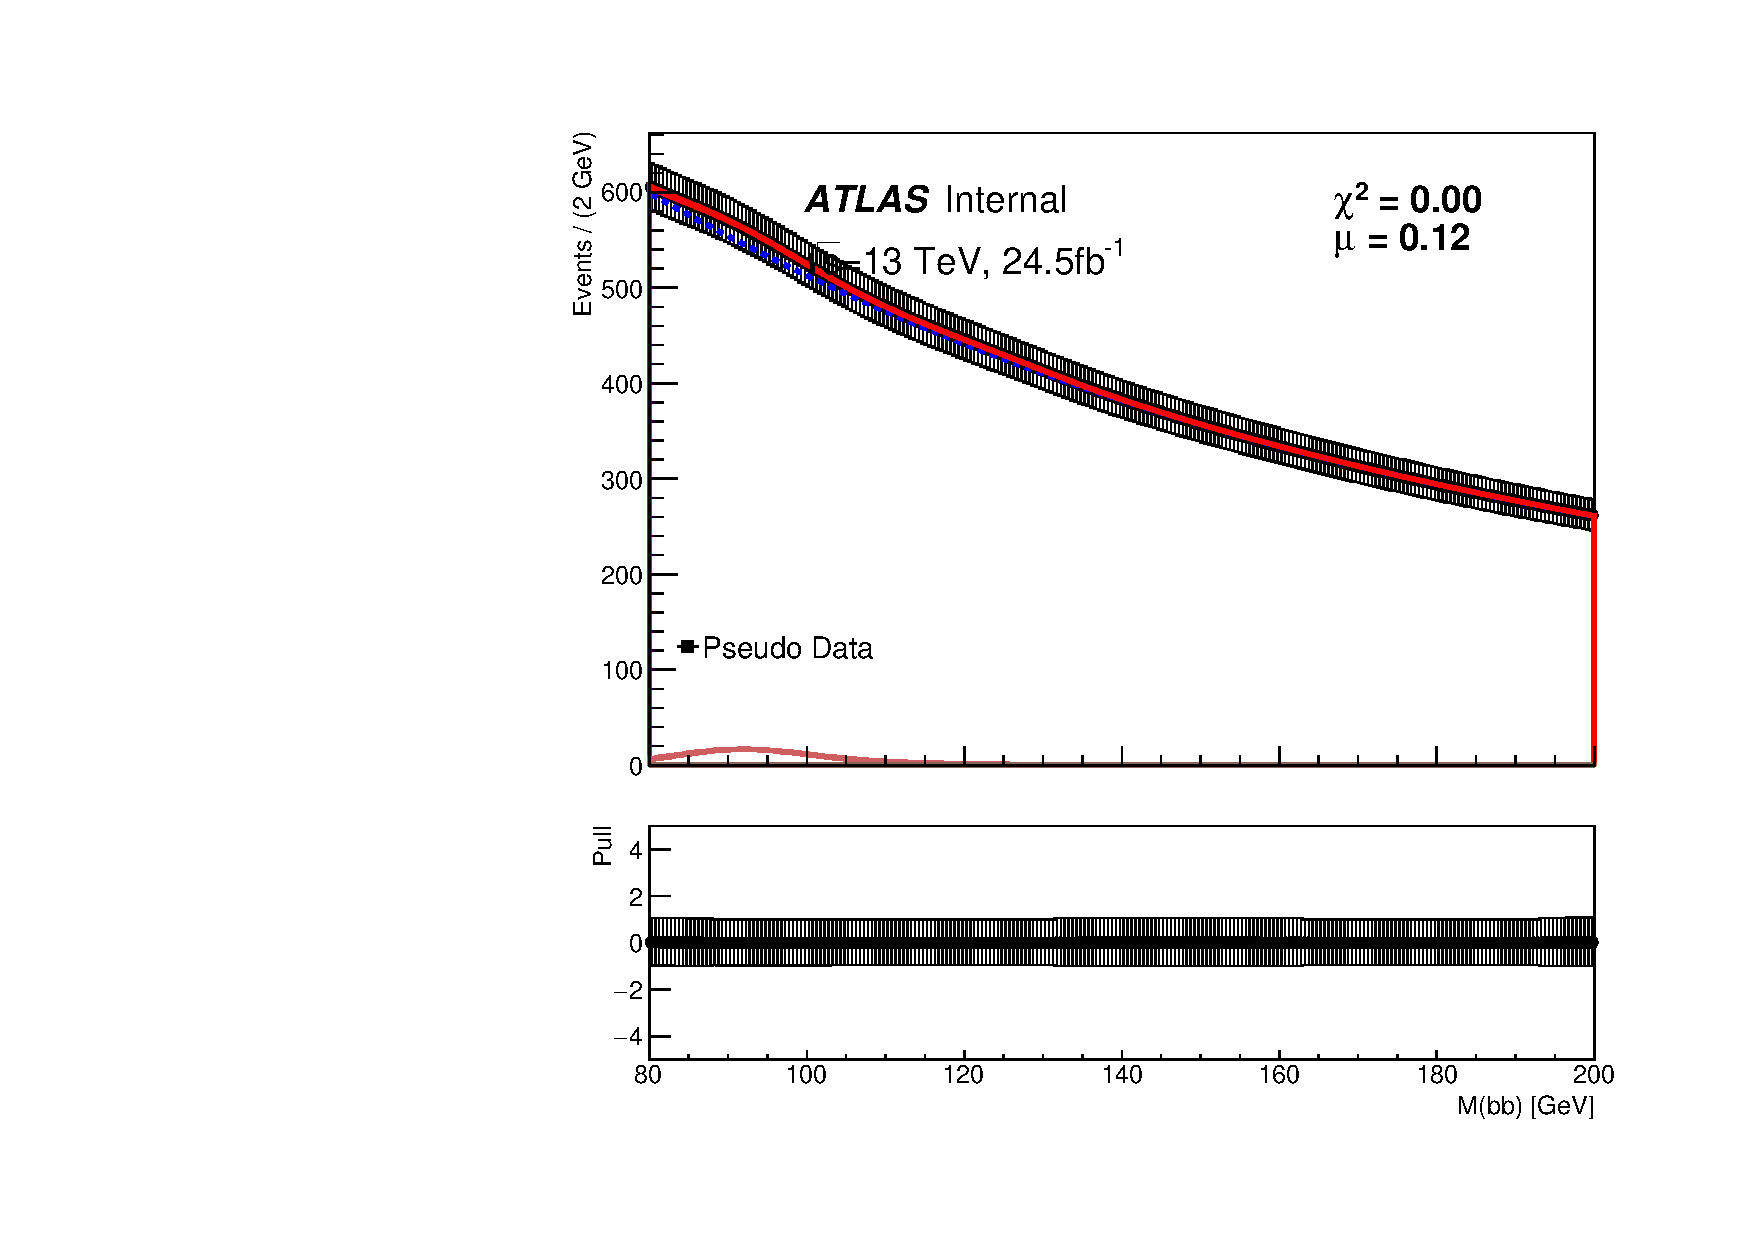
\includegraphics[width=0.24\textwidth]{figures/VBF/Spurious_ExpoO2_testVBF_ICHEP_2cen_SRI.pdf}
% 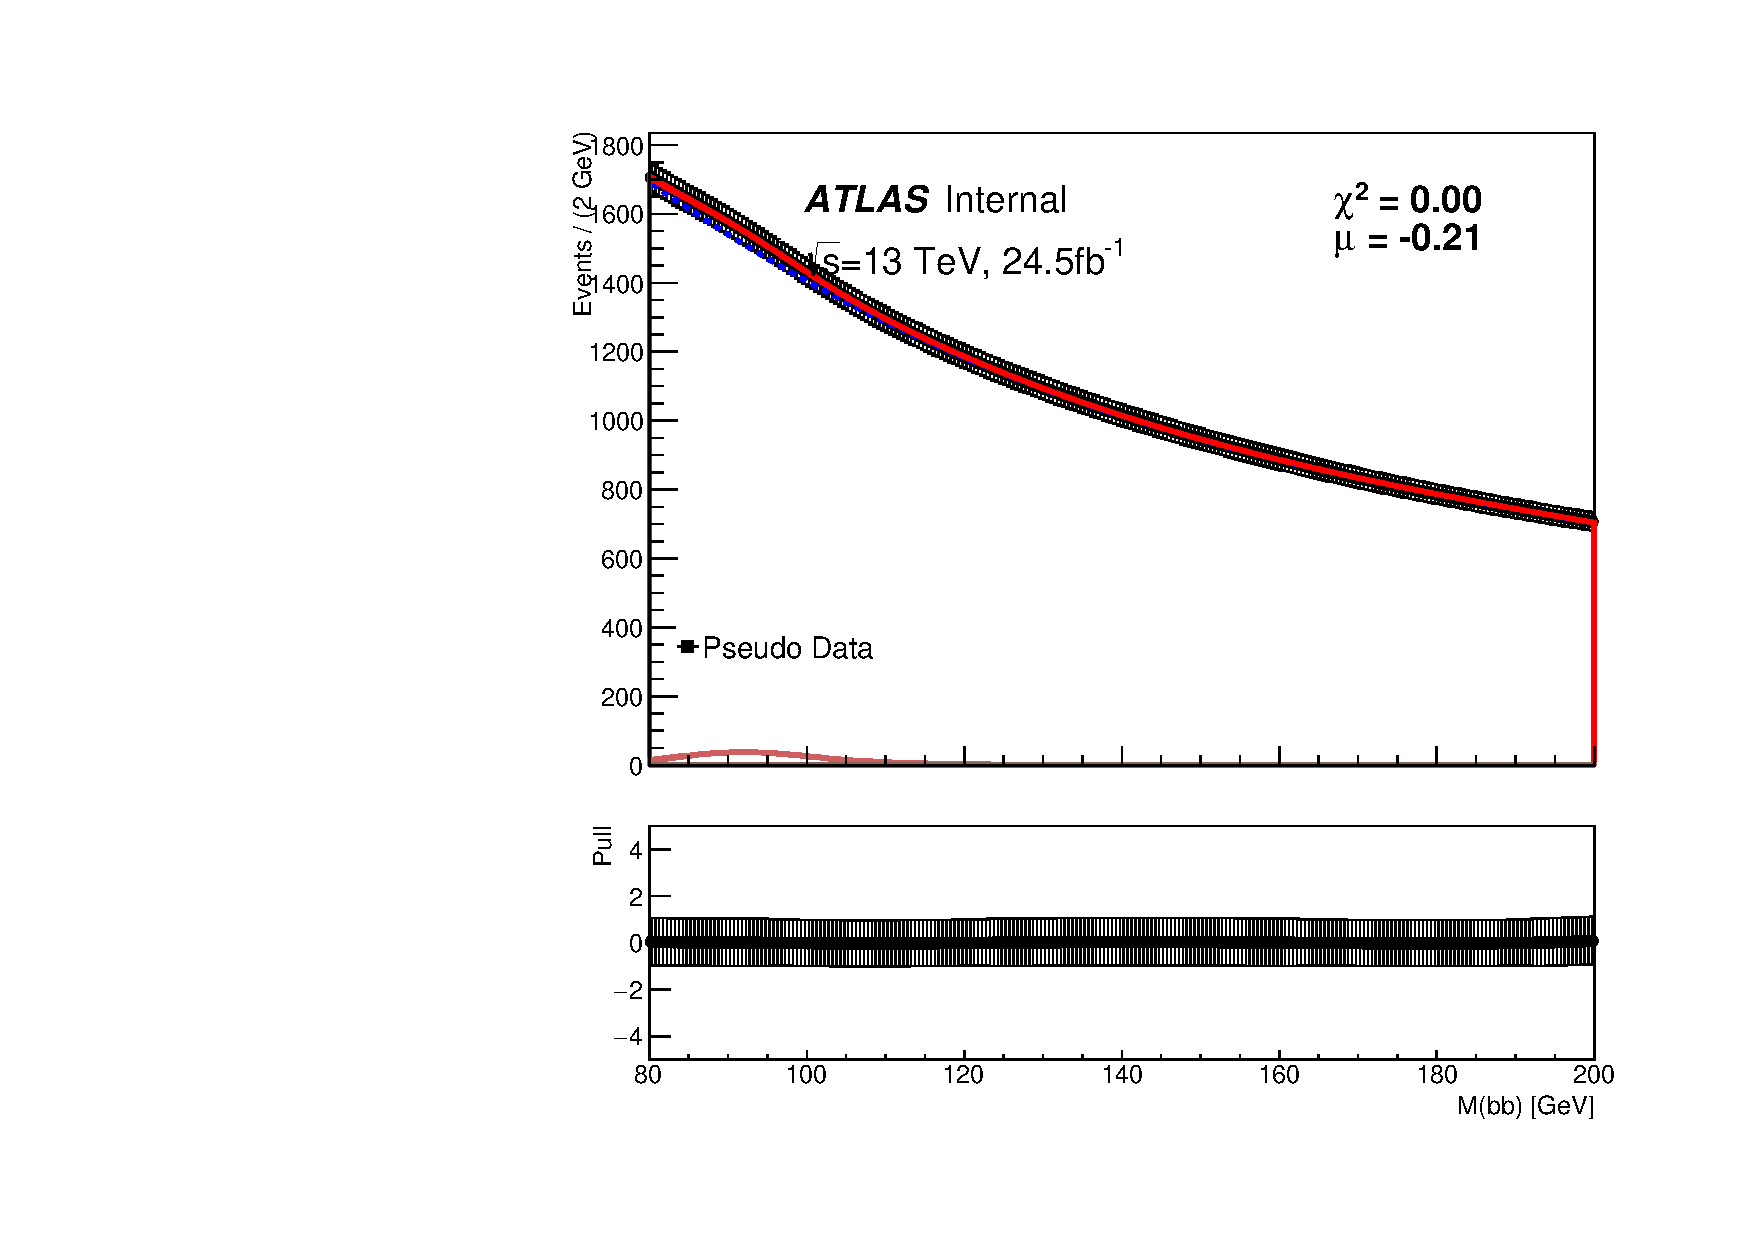
\includegraphics[width=0.24\textwidth]{figures/VBF/Spurious_ExpoO2_testVBF_ICHEP_2cen_SRII.pdf}\\
% 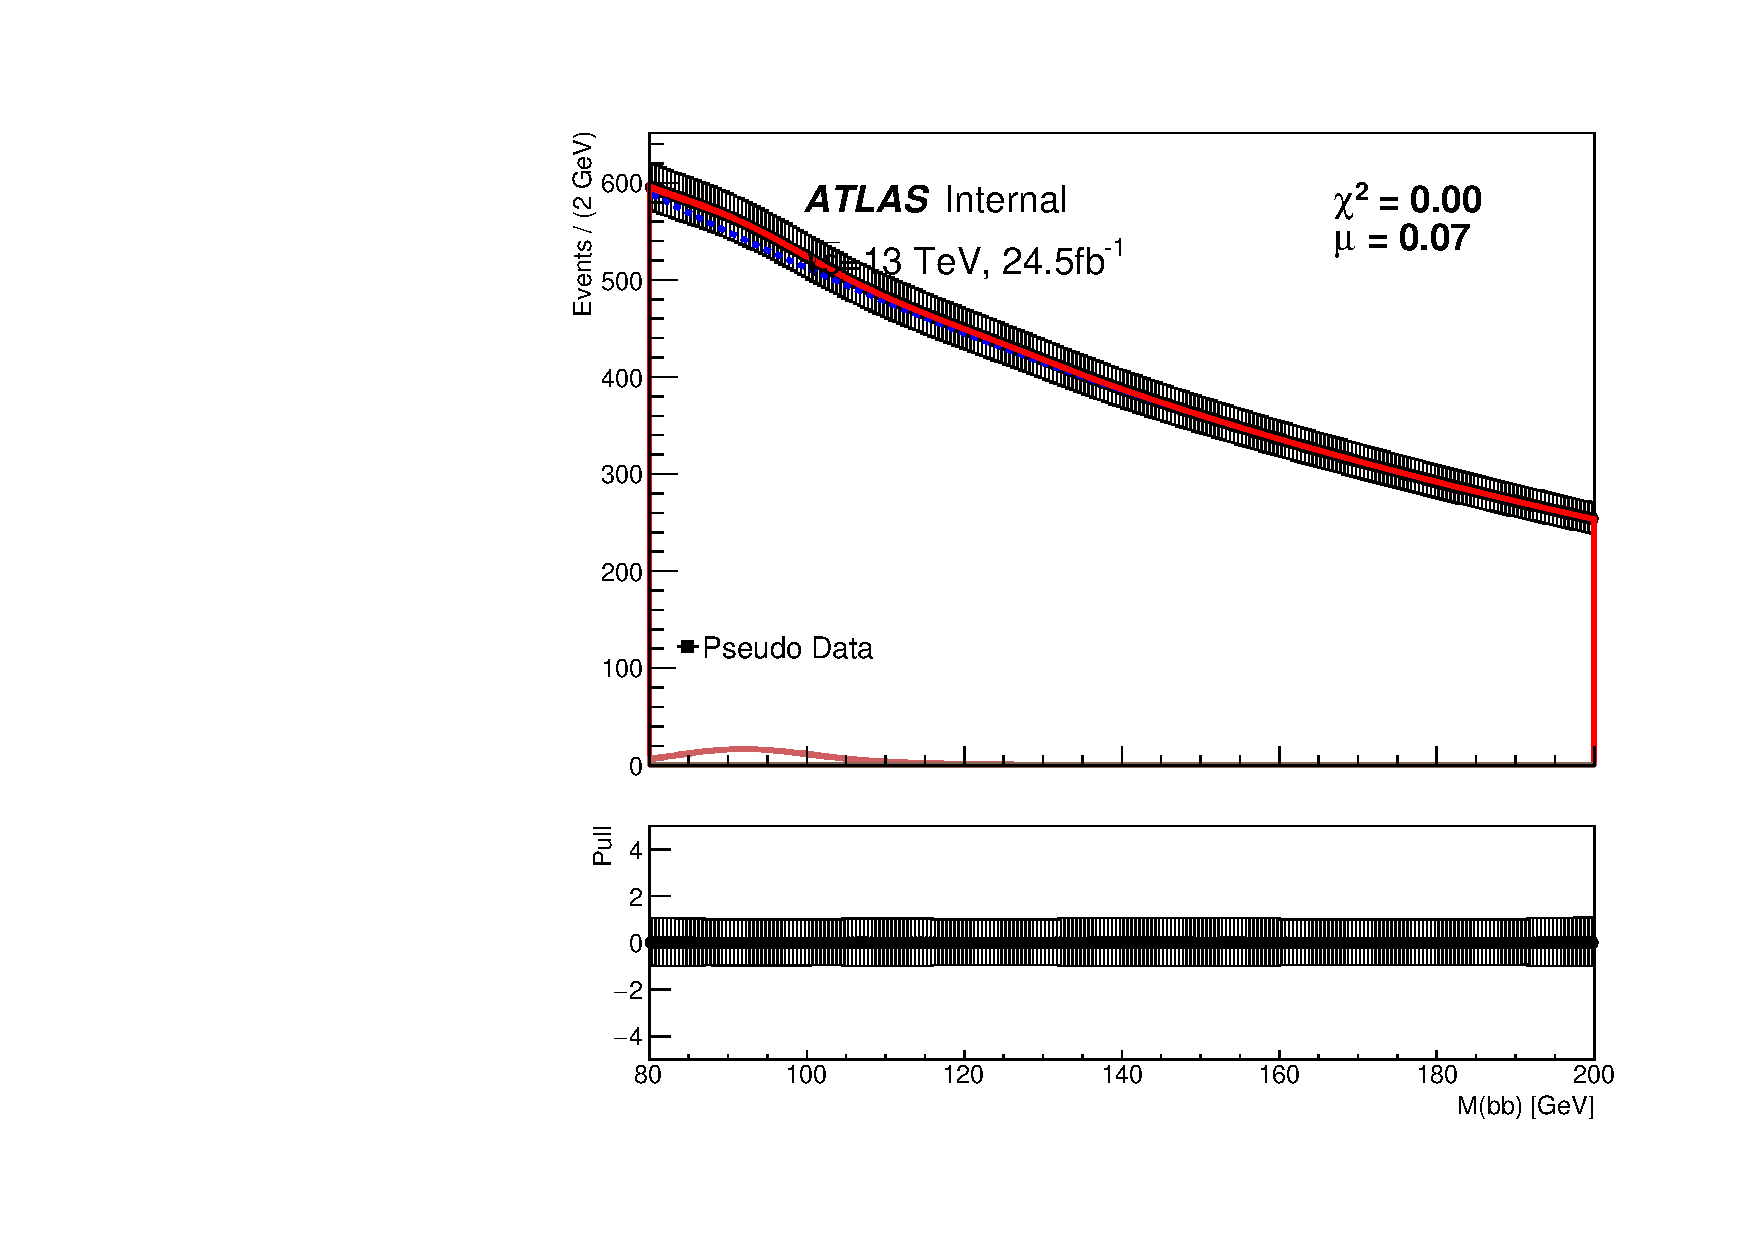
\includegraphics[width=0.24\textwidth]{figures/VBF/Spurious_SExpoO2_testVBF_ICHEP_2cen_SRI.pdf}
% 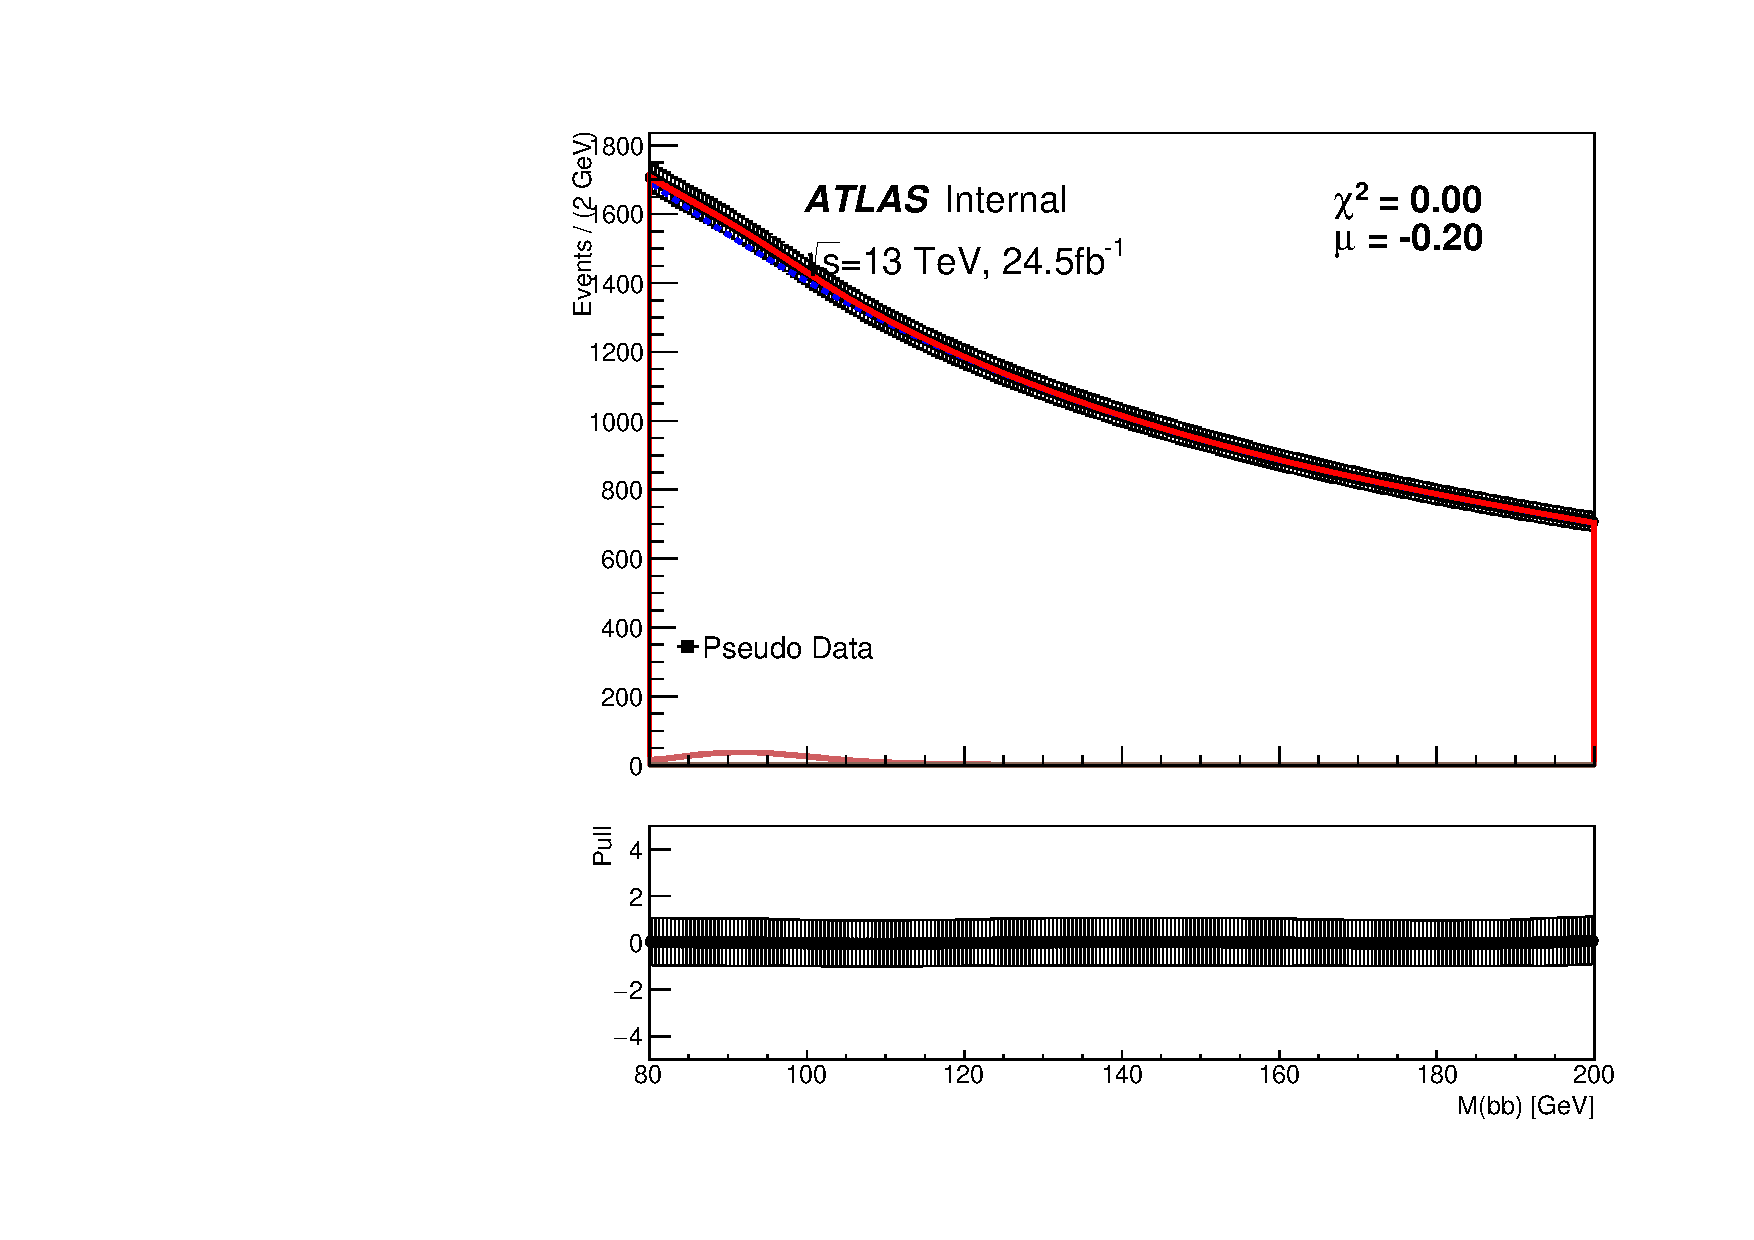
\includegraphics[width=0.24\textwidth]{figures/VBF/Spurious_SExpoO2_testVBF_ICHEP_2cen_SRII.pdf}\\
%\caption{Spurious signal fit for \twocentral channel for SR I to SR II (from left to right). The best Bernstein background models are tested against alternative truth models Expo*Bernstein O(2) (top) and Sum of Expo O(2) (bottom).}
%  \label{fig:vbf-Fit_SP_2cen}
%\end{figure}
%
%\begin{figure}[htbp]
%  \centering
% 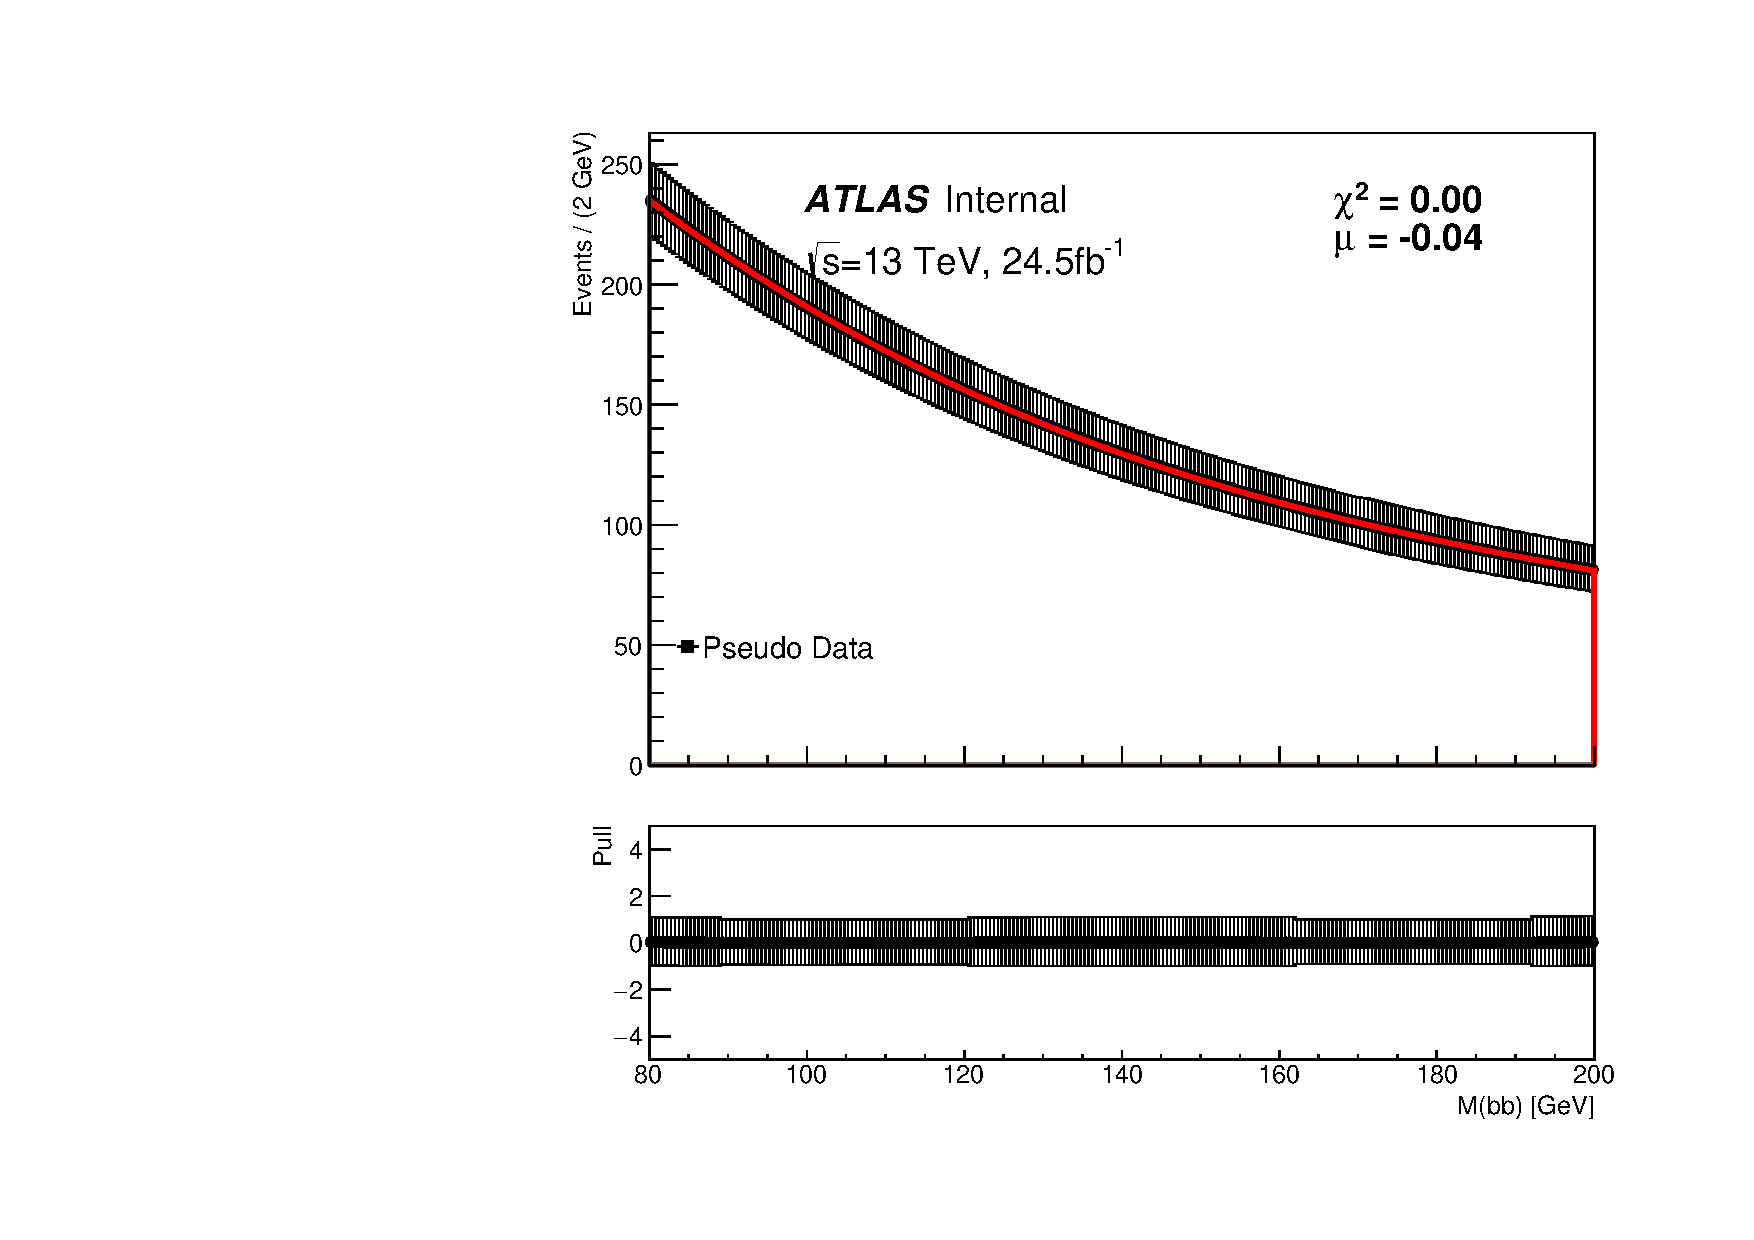
\includegraphics[width=0.24\textwidth]{figures/VBF/Spurious_ExpoO2_testVBF_ICHEP_4cen_SRI.pdf}
% 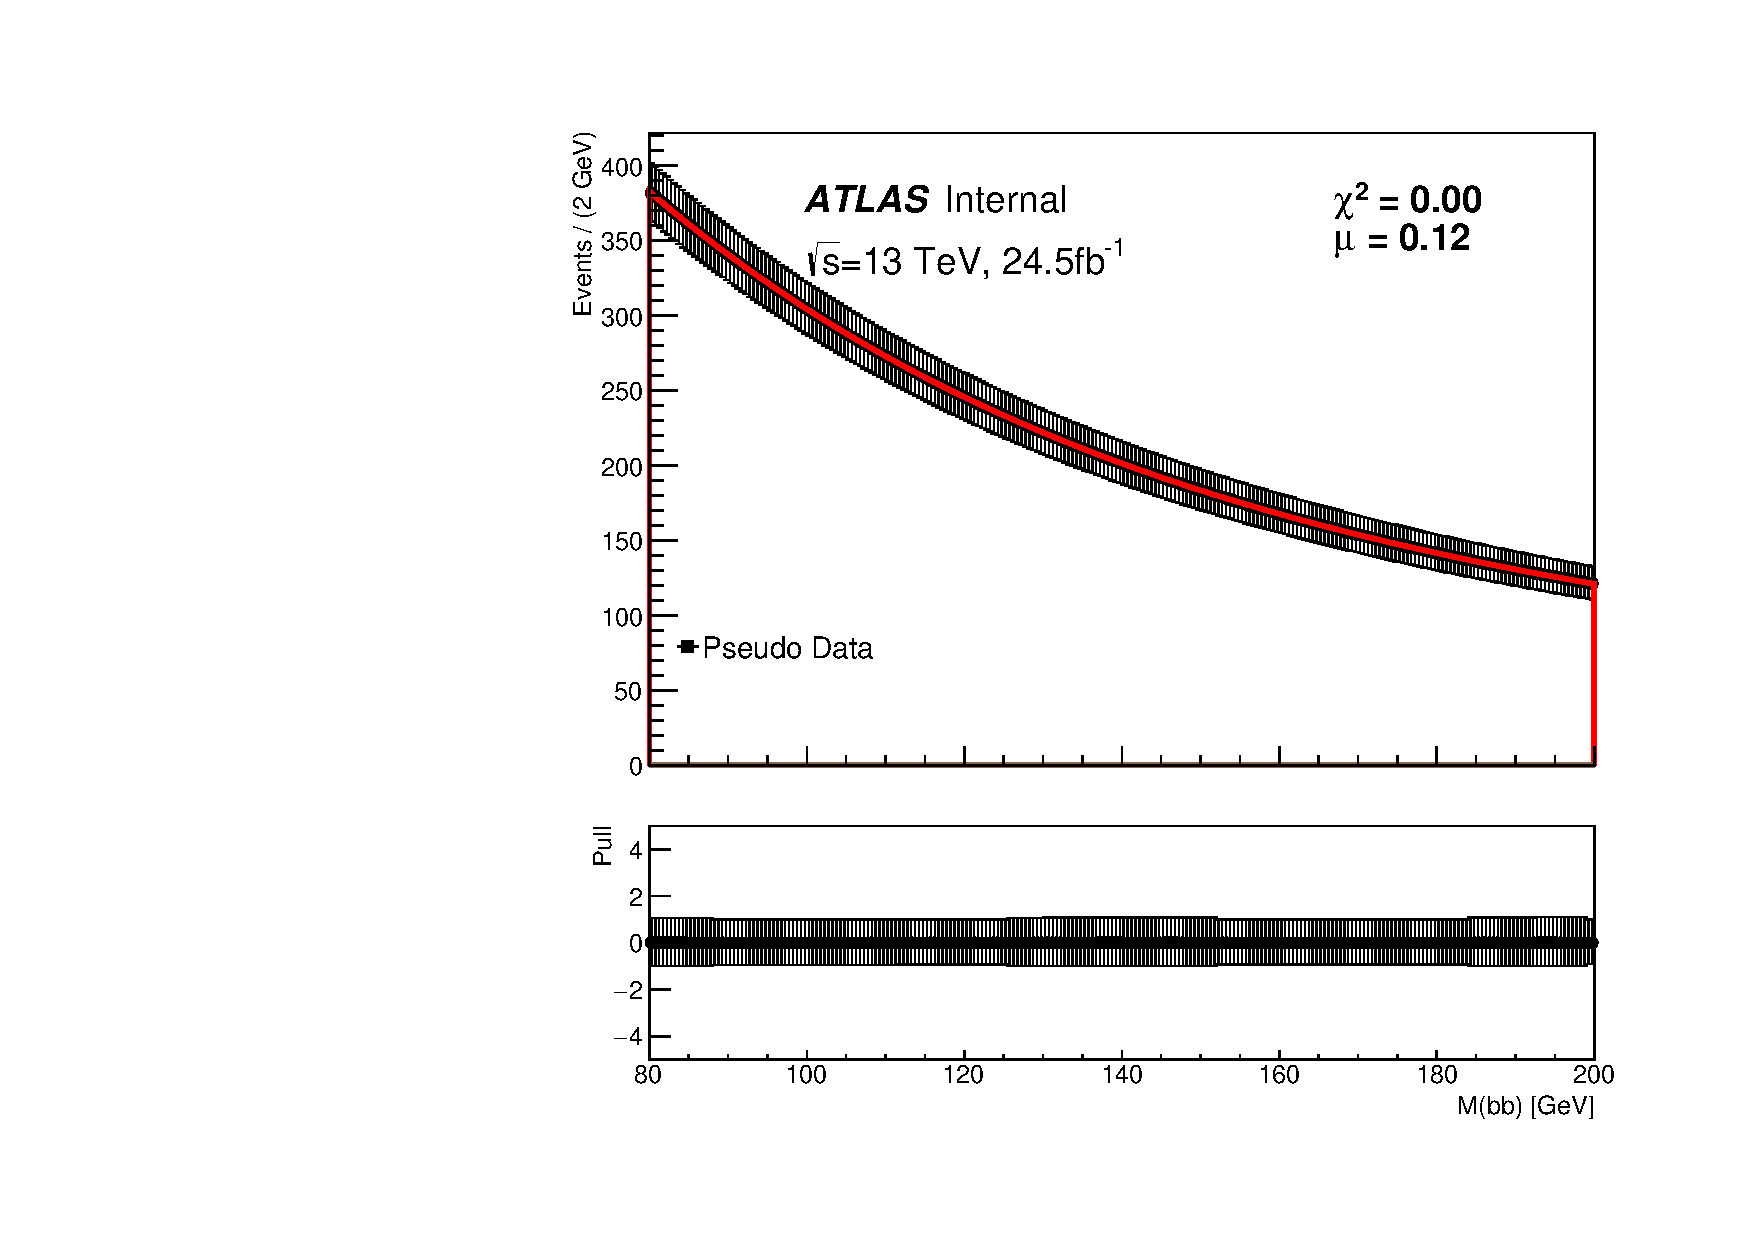
\includegraphics[width=0.24\textwidth]{figures/VBF/Spurious_ExpoO2_testVBF_ICHEP_4cen_SRII.pdf}
% 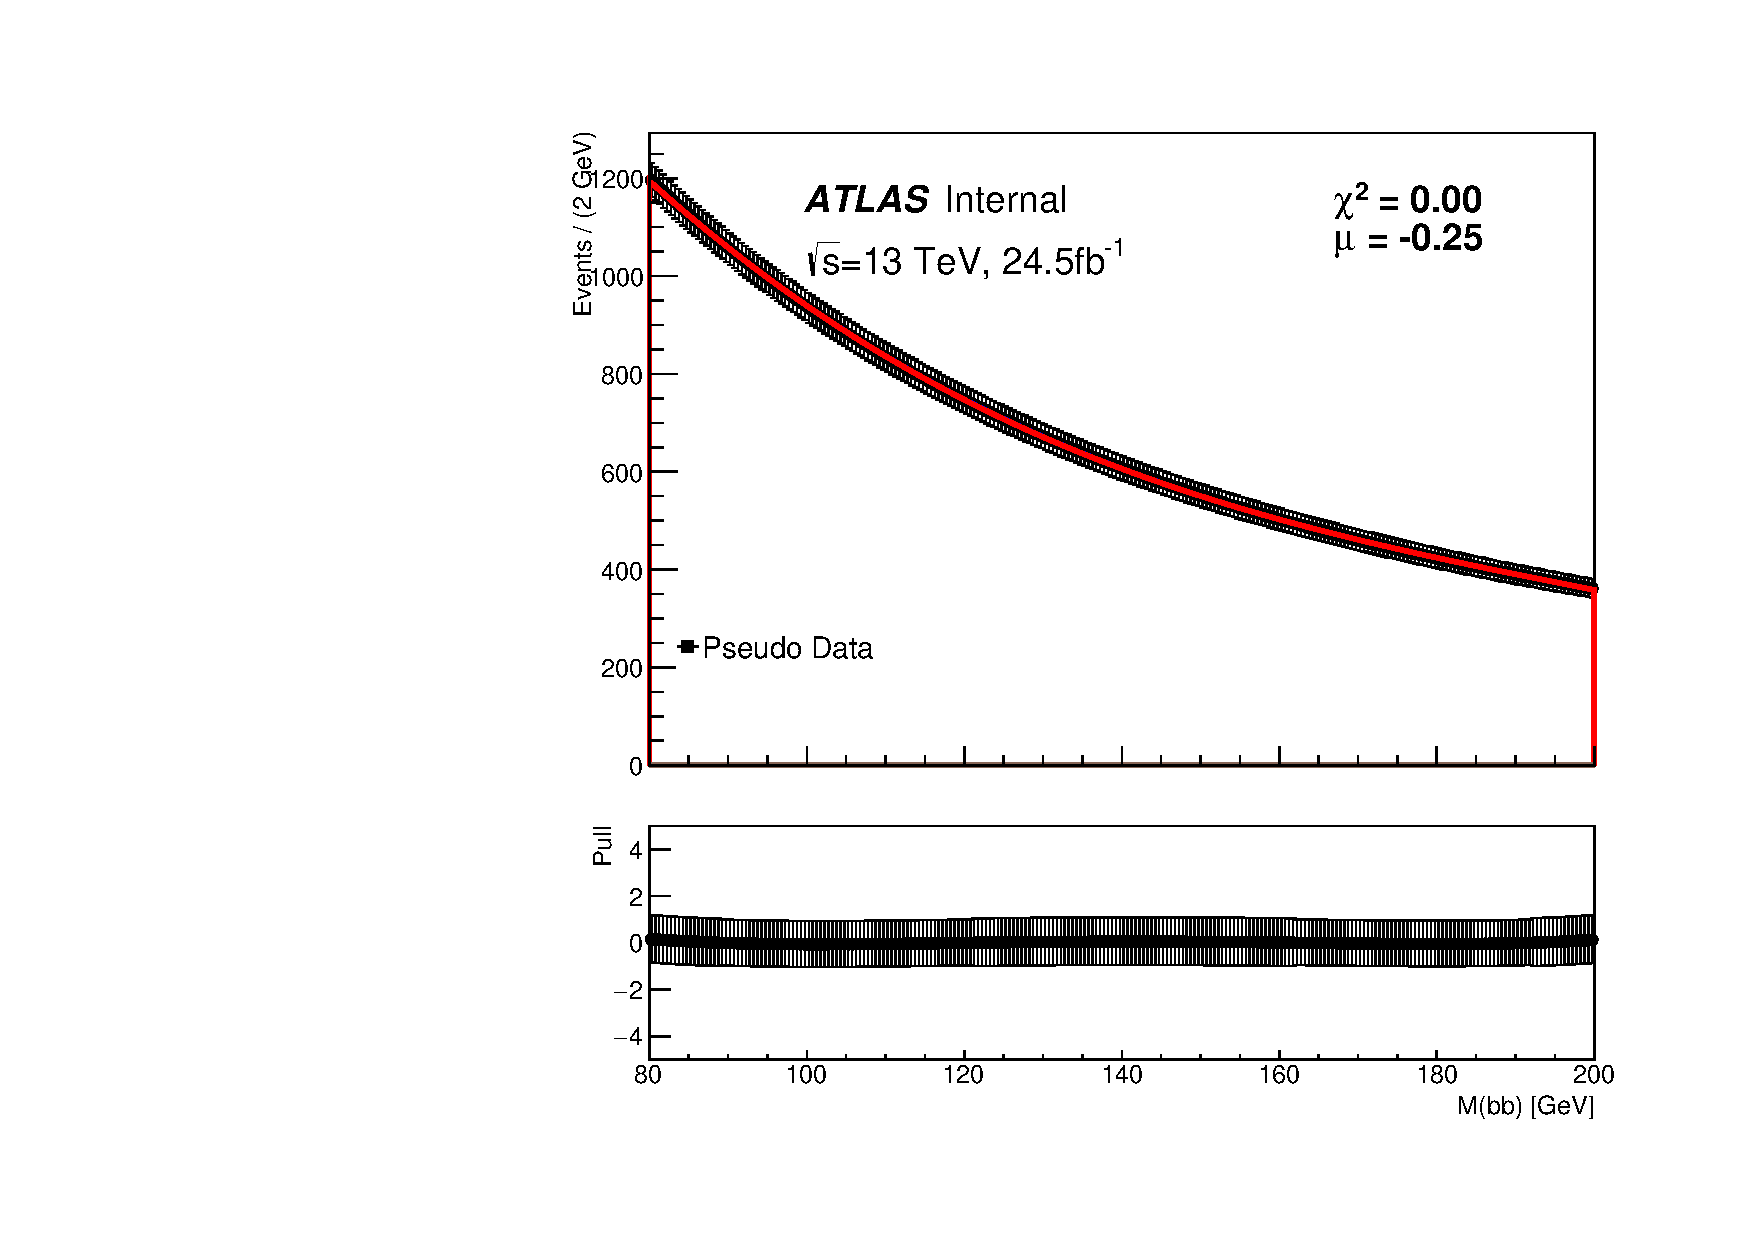
\includegraphics[width=0.24\textwidth]{figures/VBF/Spurious_ExpoO2_testVBF_ICHEP_4cen_SRIII.pdf}
% 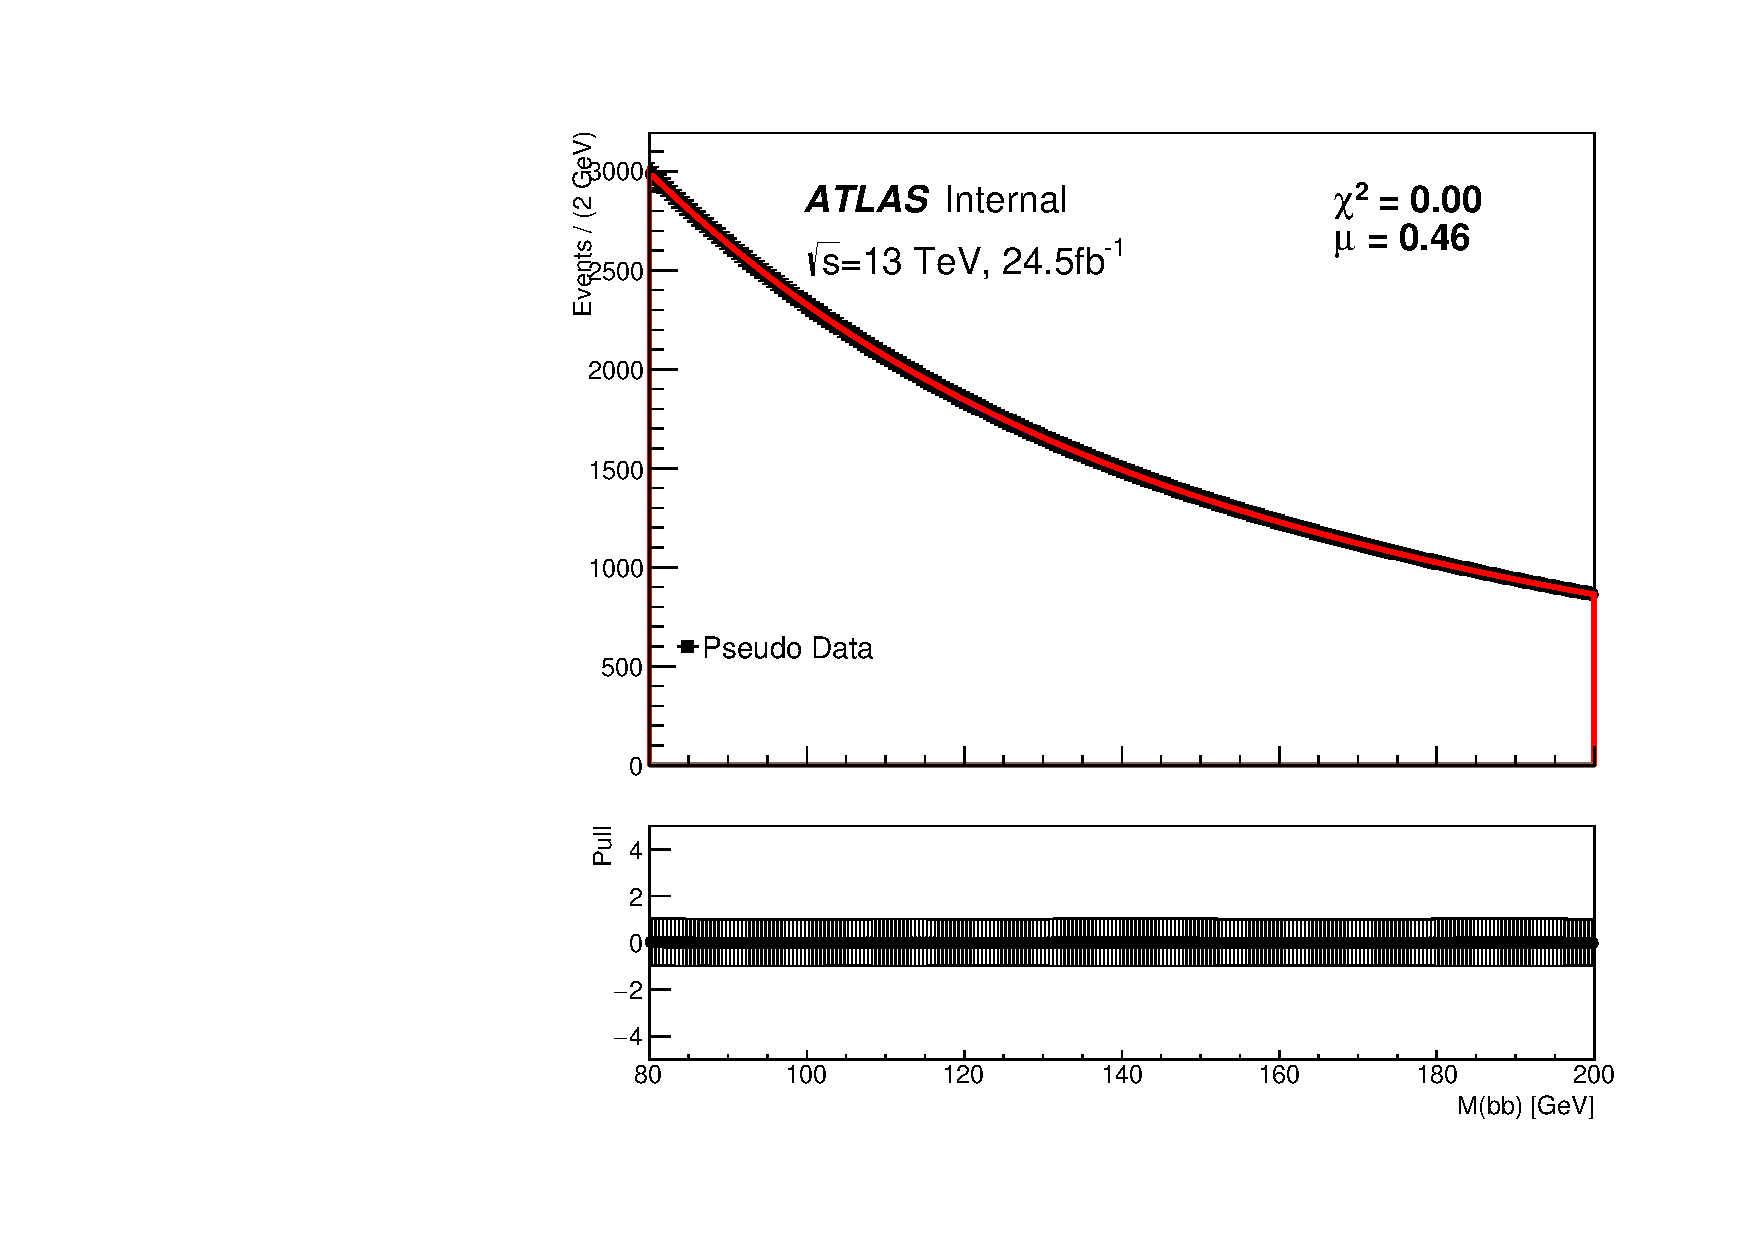
\includegraphics[width=0.24\textwidth]{figures/VBF/Spurious_ExpoO2_testVBF_ICHEP_4cen_SRIV.pdf}\\
% 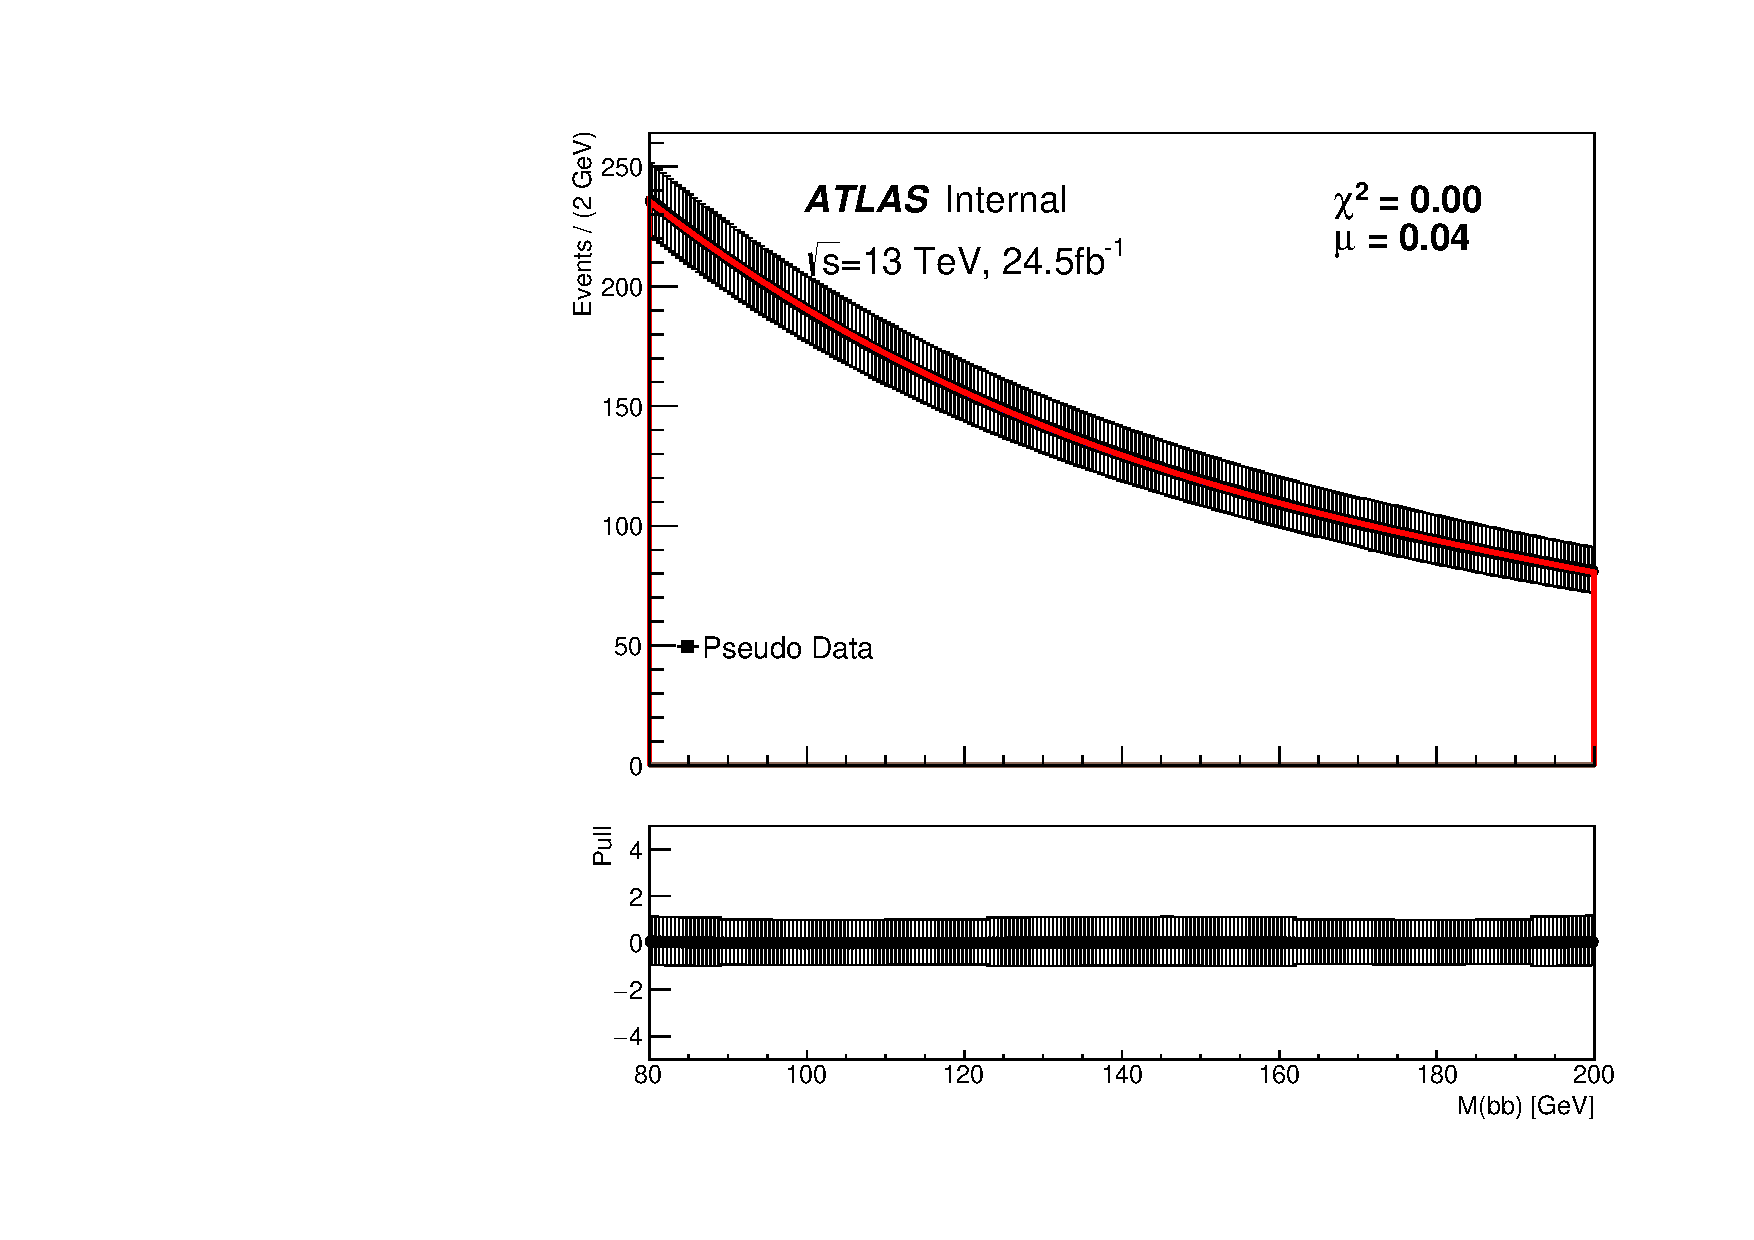
\includegraphics[width=0.24\textwidth]{figures/VBF/Spurious_SExpoO2_testVBF_ICHEP_4cen_SRI.pdf}
% 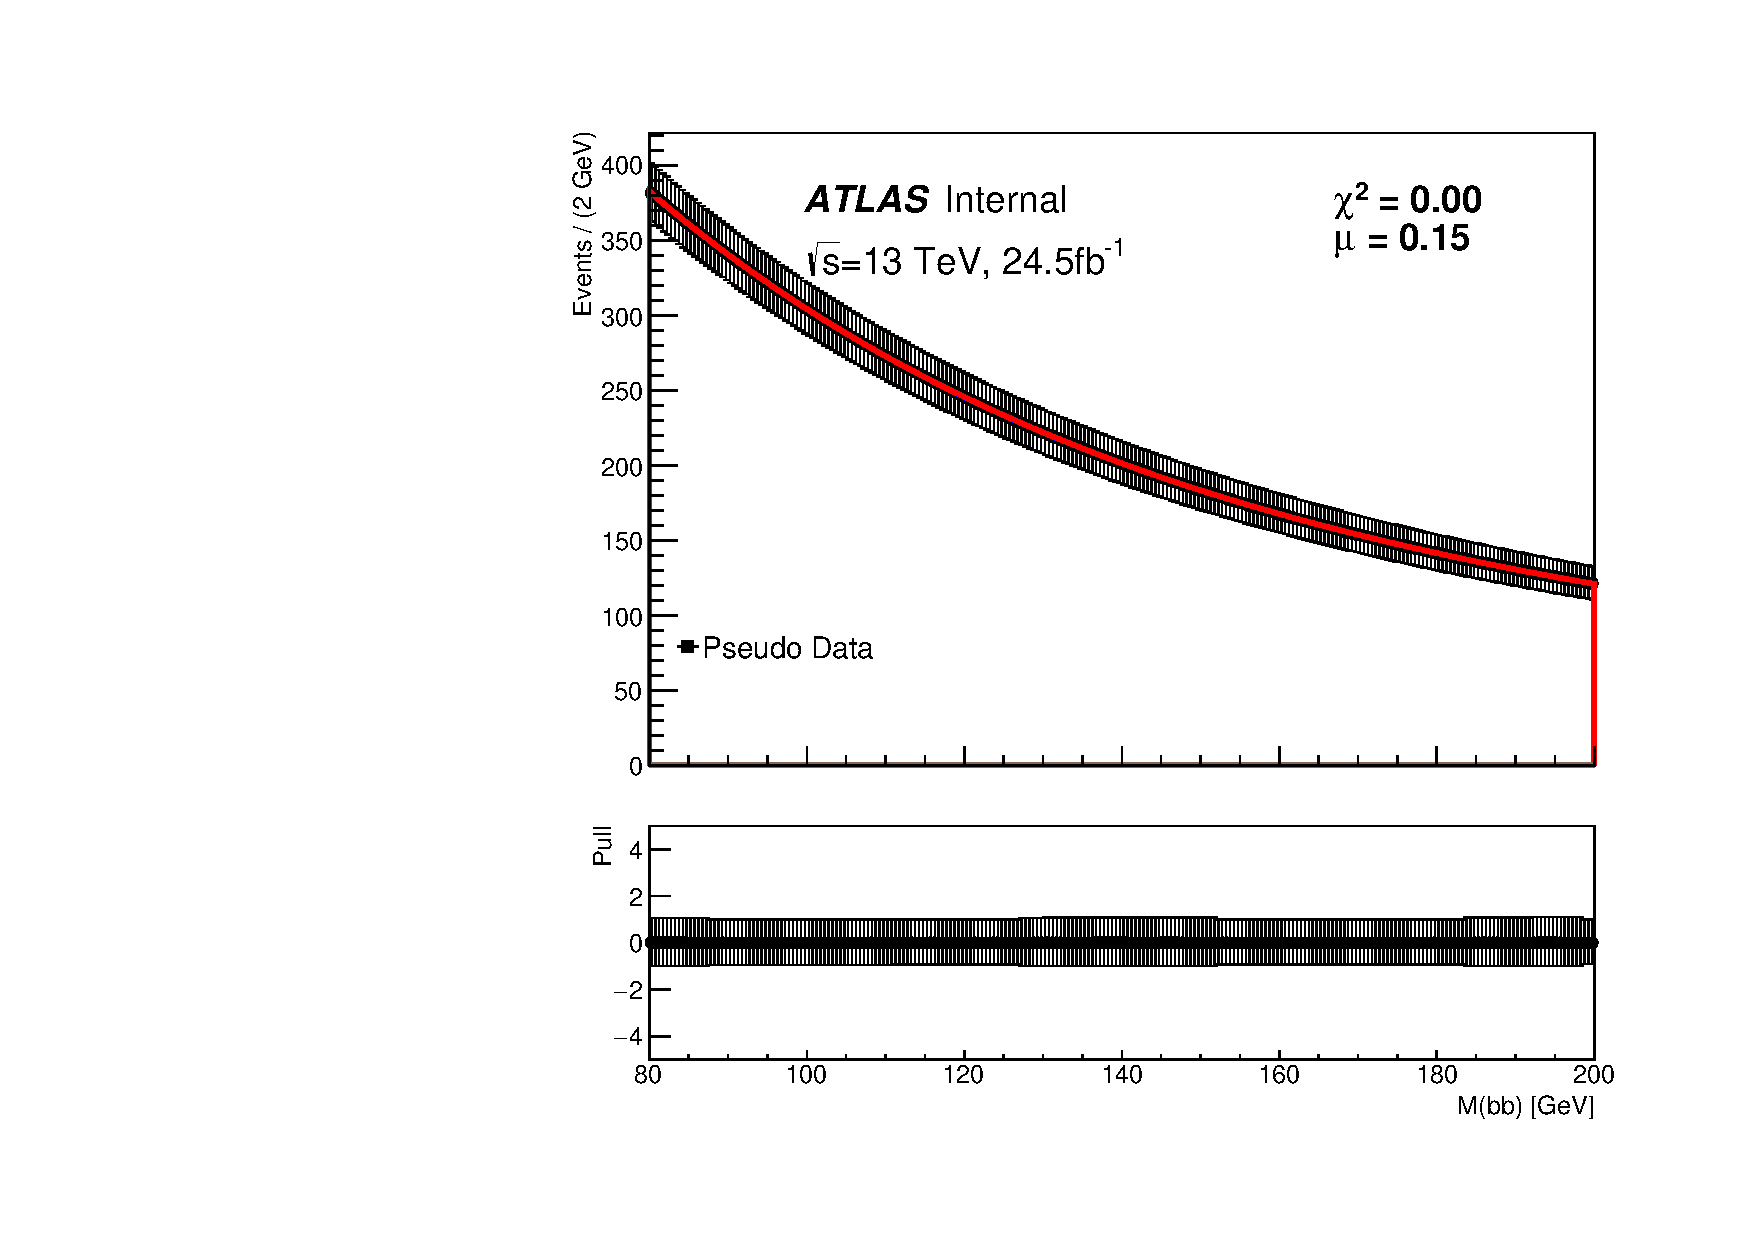
\includegraphics[width=0.24\textwidth]{figures/VBF/Spurious_SExpoO2_testVBF_ICHEP_4cen_SRII.pdf}
% 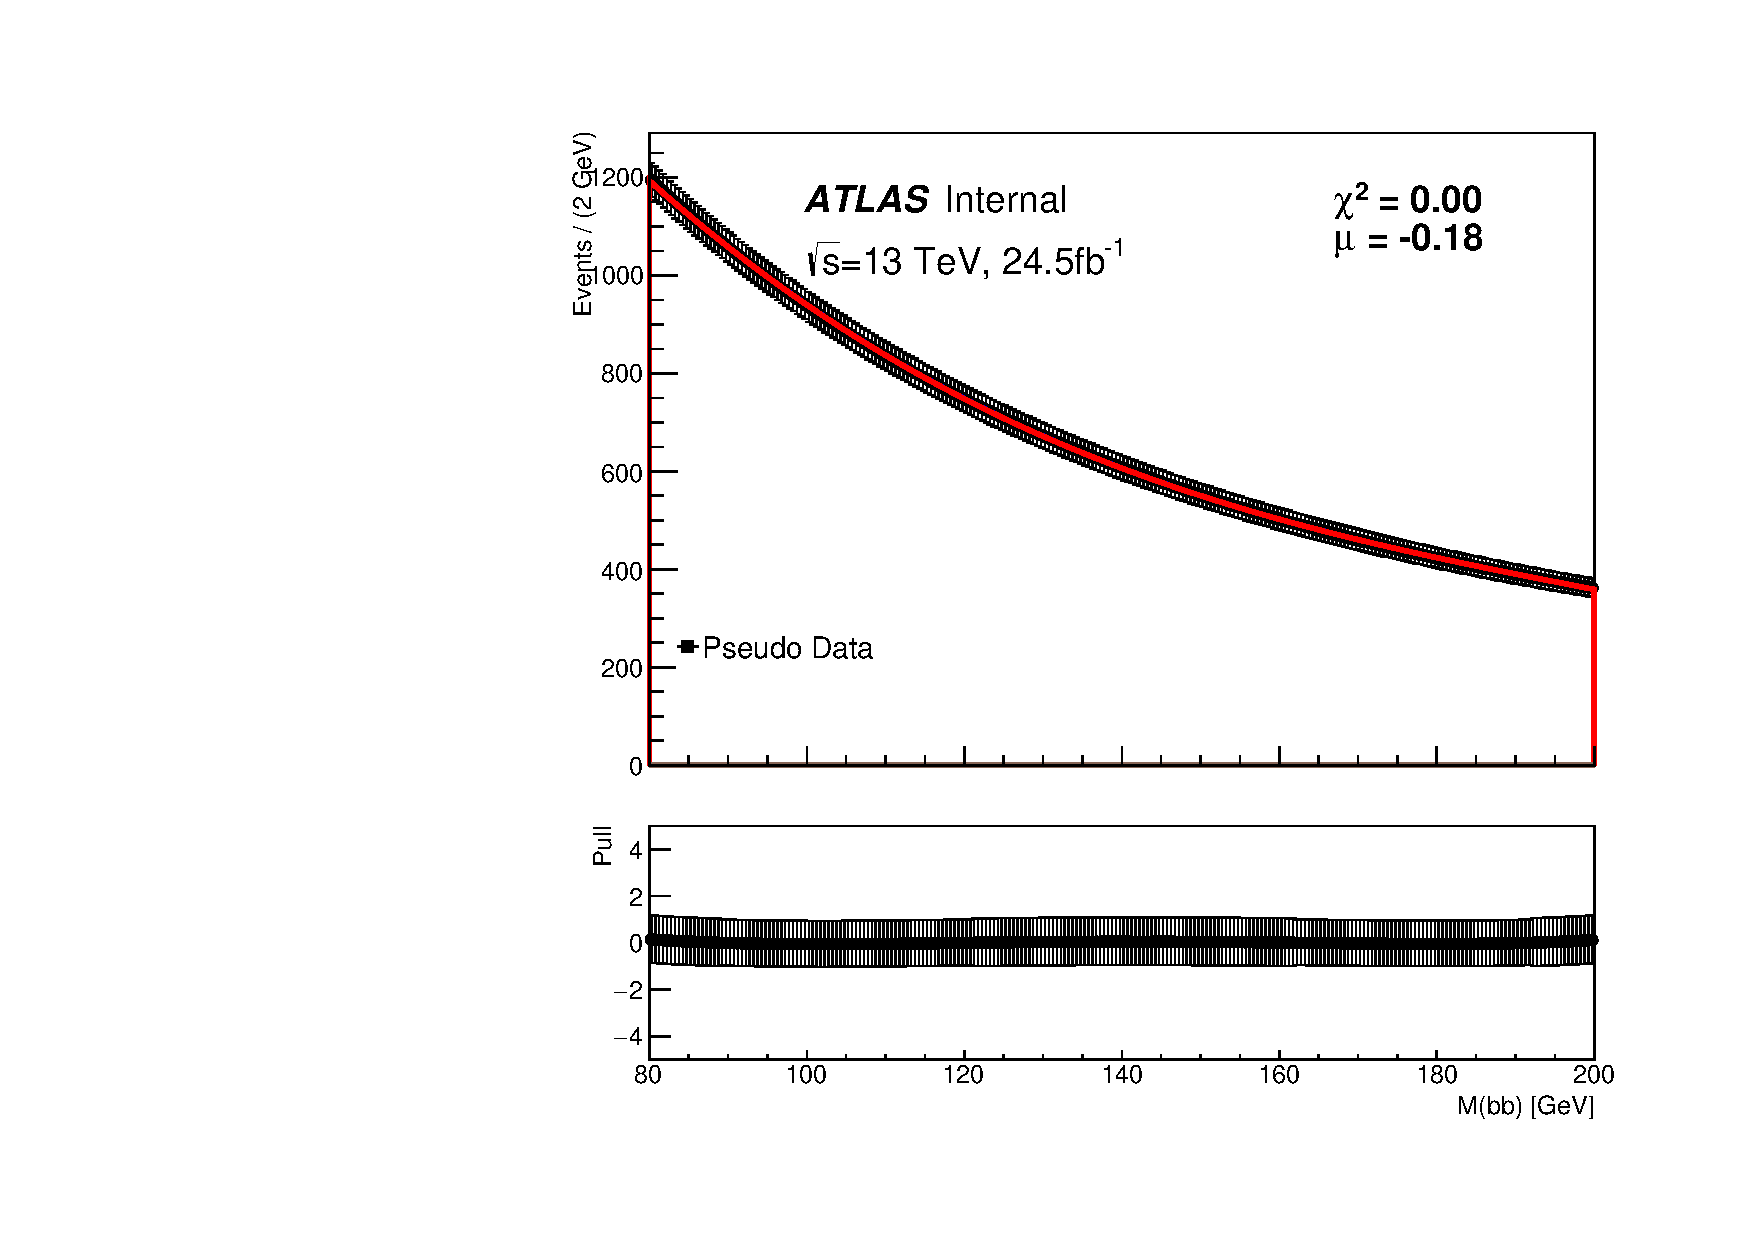
\includegraphics[width=0.24\textwidth]{figures/VBF/Spurious_SExpoO2_testVBF_ICHEP_4cen_SRIII.pdf}
% 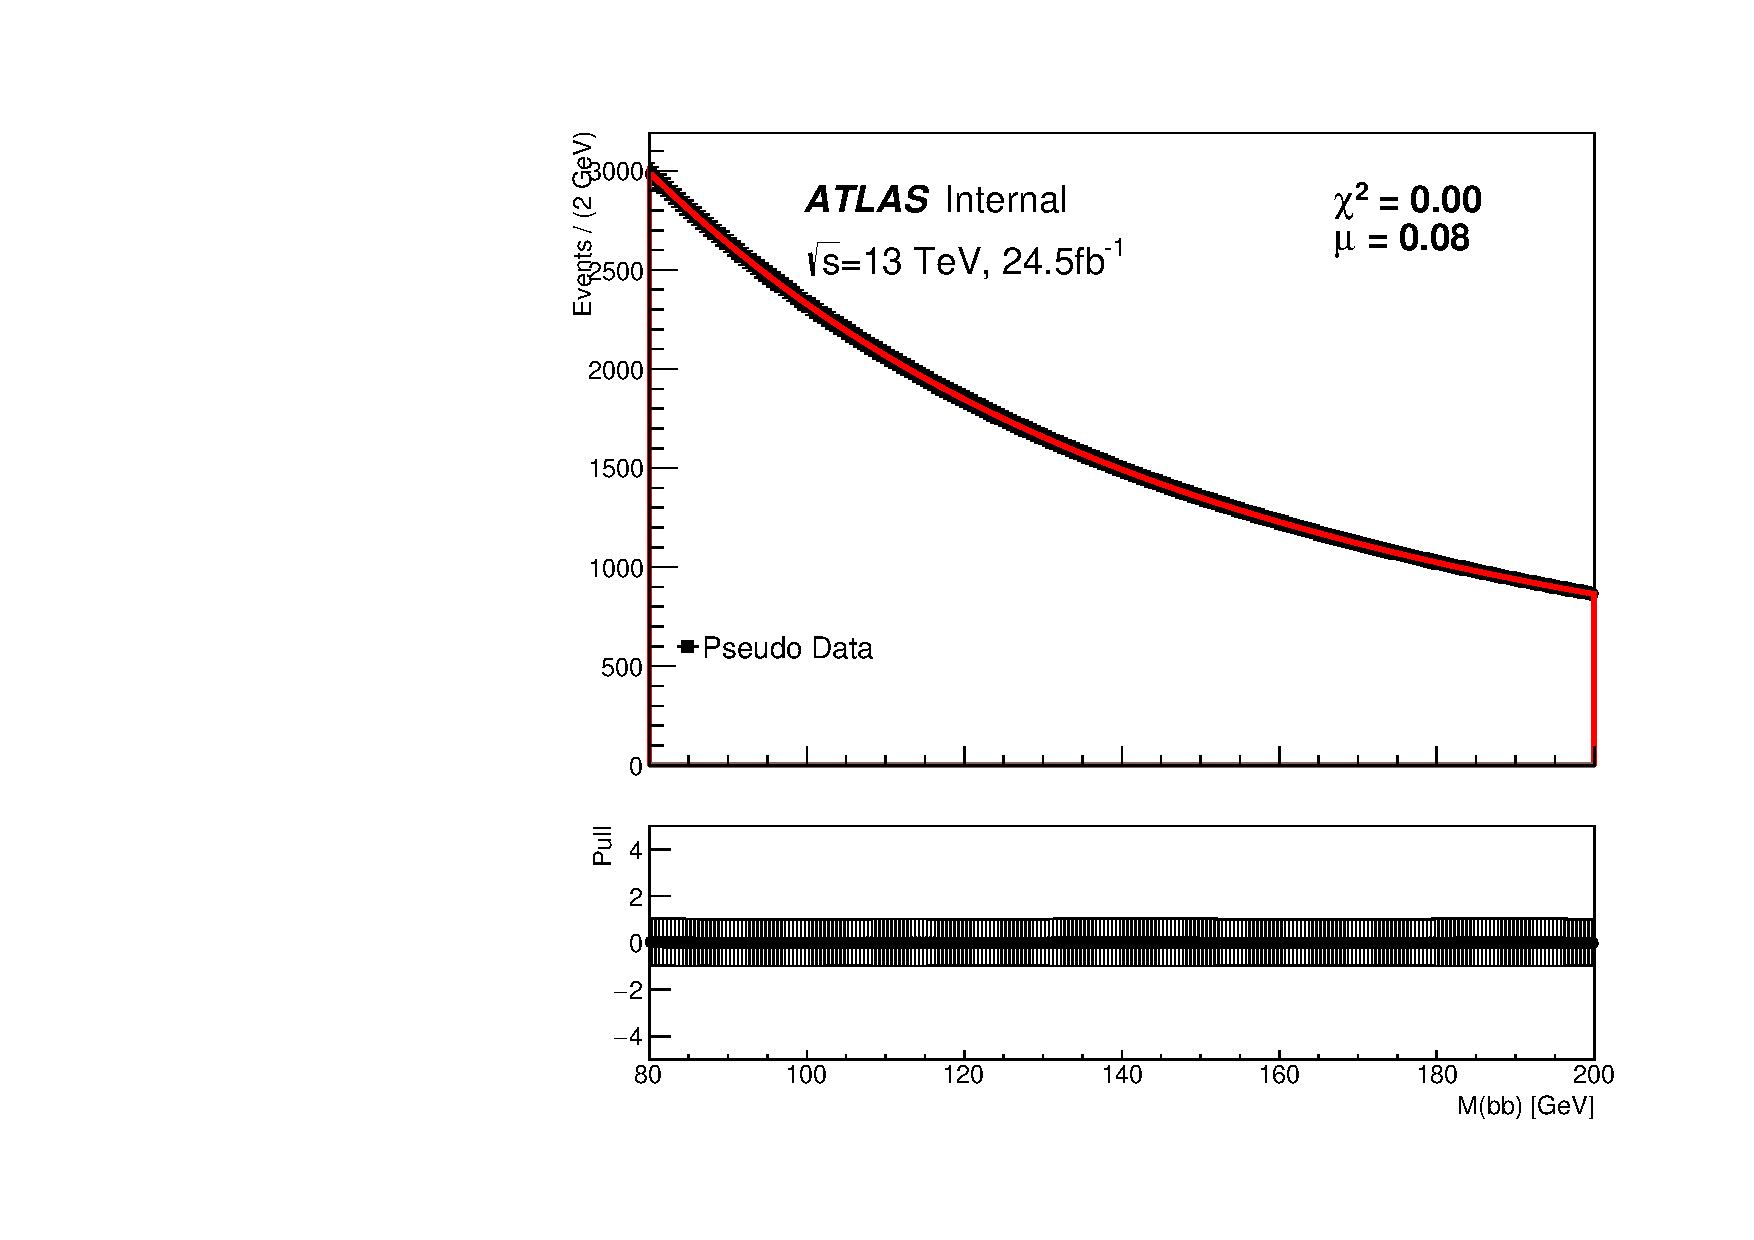
\includegraphics[width=0.24\textwidth]{figures/VBF/Spurious_SExpoO2_testVBF_ICHEP_4cen_SRIV.pdf}\\
%\caption{Spurious signal fit for \fourcentral channel for SR I to SR IV (from left to right). The best Bernstein background models are tested against alternative truth models Expo*Bernstein O(2) (top) and Sum of Expo O(2) (bottom).}
%  \label{fig:vbf-Fit_SP_4cen}
%\end{figure}



%\begin{table}[htbp]
%\centering
%\caption{Higgs sensitivity of each channel quantified in $\Delta \mu$ for different orders of non-resonant background function choice}
%\label{tab:perchannel_sensitivity}
%\begin{tabular}{|c|c|c|c|}
%\hline
%Channel      & Bernstein O2 & Bernstein O3 & Bernstein O4 \\ \hline
%2cen, SR I   & 2.09         & 2.67         &              \\ \hline
%2cen, SR II  & 5.50         & 8.09         &              \\ \hline
%4cen, SR I   & 2.86         & 3.60         &              \\ \hline
%4cen, SR II  & 6.44         & 9.32         & 10.07        \\ \hline
%4cen, SR III & 5.23         & 7.01         &              \\ \hline
%4cen, SR IV  & 4.20         & 5.51         & 5.89         \\ \hline
%\end{tabular}
%\end{table}


%You can find some text snippets that can be used in papers in \texttt{template/atlas-snippets.tex}.
%Some of the snippets need the \texttt{jetetmiss} option passed to \texttt{atlasphysics}.
%\input{atlas-snippets}
%You can find some text snippets that can be used in papers in \texttt{template/atlas-snippets.tex}.
%Some of the snippets need the \texttt{jetetmiss} option passed to \texttt{atlasphysics}.
%\input{atlas-snippets}
%-------------------------------------------------------------------------------
\subsection{Results}
\label{sec:result}
%-------------------------------------------------------------------------------
The VBF \Hbb analysis unblinding proceeds in two steps. First, overall strategy is validated with a fit to the $Z$ contribution in a sideband only fit while the Higgs mass window is kept unblinded, shown in Section~\ref{sec:vbf-zunblind}.  Then a simultaneous fit to the signal, correlated over all signal regions, and the $Z$ signal, uncorrelated across signal regions, is done over the entire mass region, as described in~\ref{sec:vbf-higgsunblind}. As an alternative interpretation of this analysis the $\mu_{VBF}$ strength is extracted by only allowing $VBF$ events to float in the fit and fixing all other Higgs processes, i.e. ggF, ttH and VH, to Standard Model expectation, as described in~\ref{sec:vbf-higgsunblindvbf}. The combination of inclusive $VBF$ and $VBF+\gamma$ results are presented in~\ref{sec:vbf-higgscomb}.


\subsection{Unblinding of \zjets{} in mass sidebands}
\label{sec:vbf-zunblind}

The fit strategy is first validated in data with a closure obtained in \zjets{} mass sideband fit. We performed a side-band only fit to extract the \zjets{} contribution independently in all regions. The fitted \zjets{} strengths are summarized in Table~\ref{tab:zsidebandfit}, presented with with all experimental and statistical uncertainties.   Note that we have no BDT shape uncertainties on the \zjets{} MC so cannot draw any conclusions from the compatibility of $\mu_Z$ with 1 in the different BDT regions. The effective $\mu_{Z}^{\rm eff}$ of all regions combined is defined as
\begin{equation}
\label{eqn:zsig}
\mu_{Z}^{\rm eff} = \sum \mu_{Z,i}\frac{n_{Z,i}}{\sum n_{Z,i}} 
\end{equation}
where $n_{Z,i}$ is the number of $Z$ events in region $i$, and $\mu_{Z,i}$ is the measured $\mu_Z$ in region $i$.  $\mu_{Z}^{\rm eff}$ is measured to be $1.0\pm 0.4$ in the sideband only fit with a compatibility of $\chi^2/nodf = 5.5/6=0.9$ ($\chi^2$ probability of 48\%).


\begin{table}[htbp]
\centering
\caption{Floating Z normalization parameters in data sideband fit including all systematic uncertainties.}
\label{tab:zsidebandfit}
\begin{tabular}{|l|c|c|}
\hline
Channel      & $\mu_{Z}$   & $\chi^2/ndof$ \\ \hline
2 cen SR I   & 2.6 $\pm$1.3  & 1.1          \\ \hline
2 cen SR II  & 0.4$\pm$0.8  & 0.7          \\ \hline
4 cen SR I   & 2.2$\pm$2.0  & 0.8          \\ \hline
4 cen SR II  & 2.0$\pm$1.9  & 0.9          \\ \hline
4 cen SR III & 1.9$\pm$0.6  & 0.9          \\ \hline
4 cen SR IV  & 0.6$\pm$0.6  & 0.9          \\ \hline
\end{tabular}
\end{table}



%\begin{figure}[htbp]
%  \centering
% 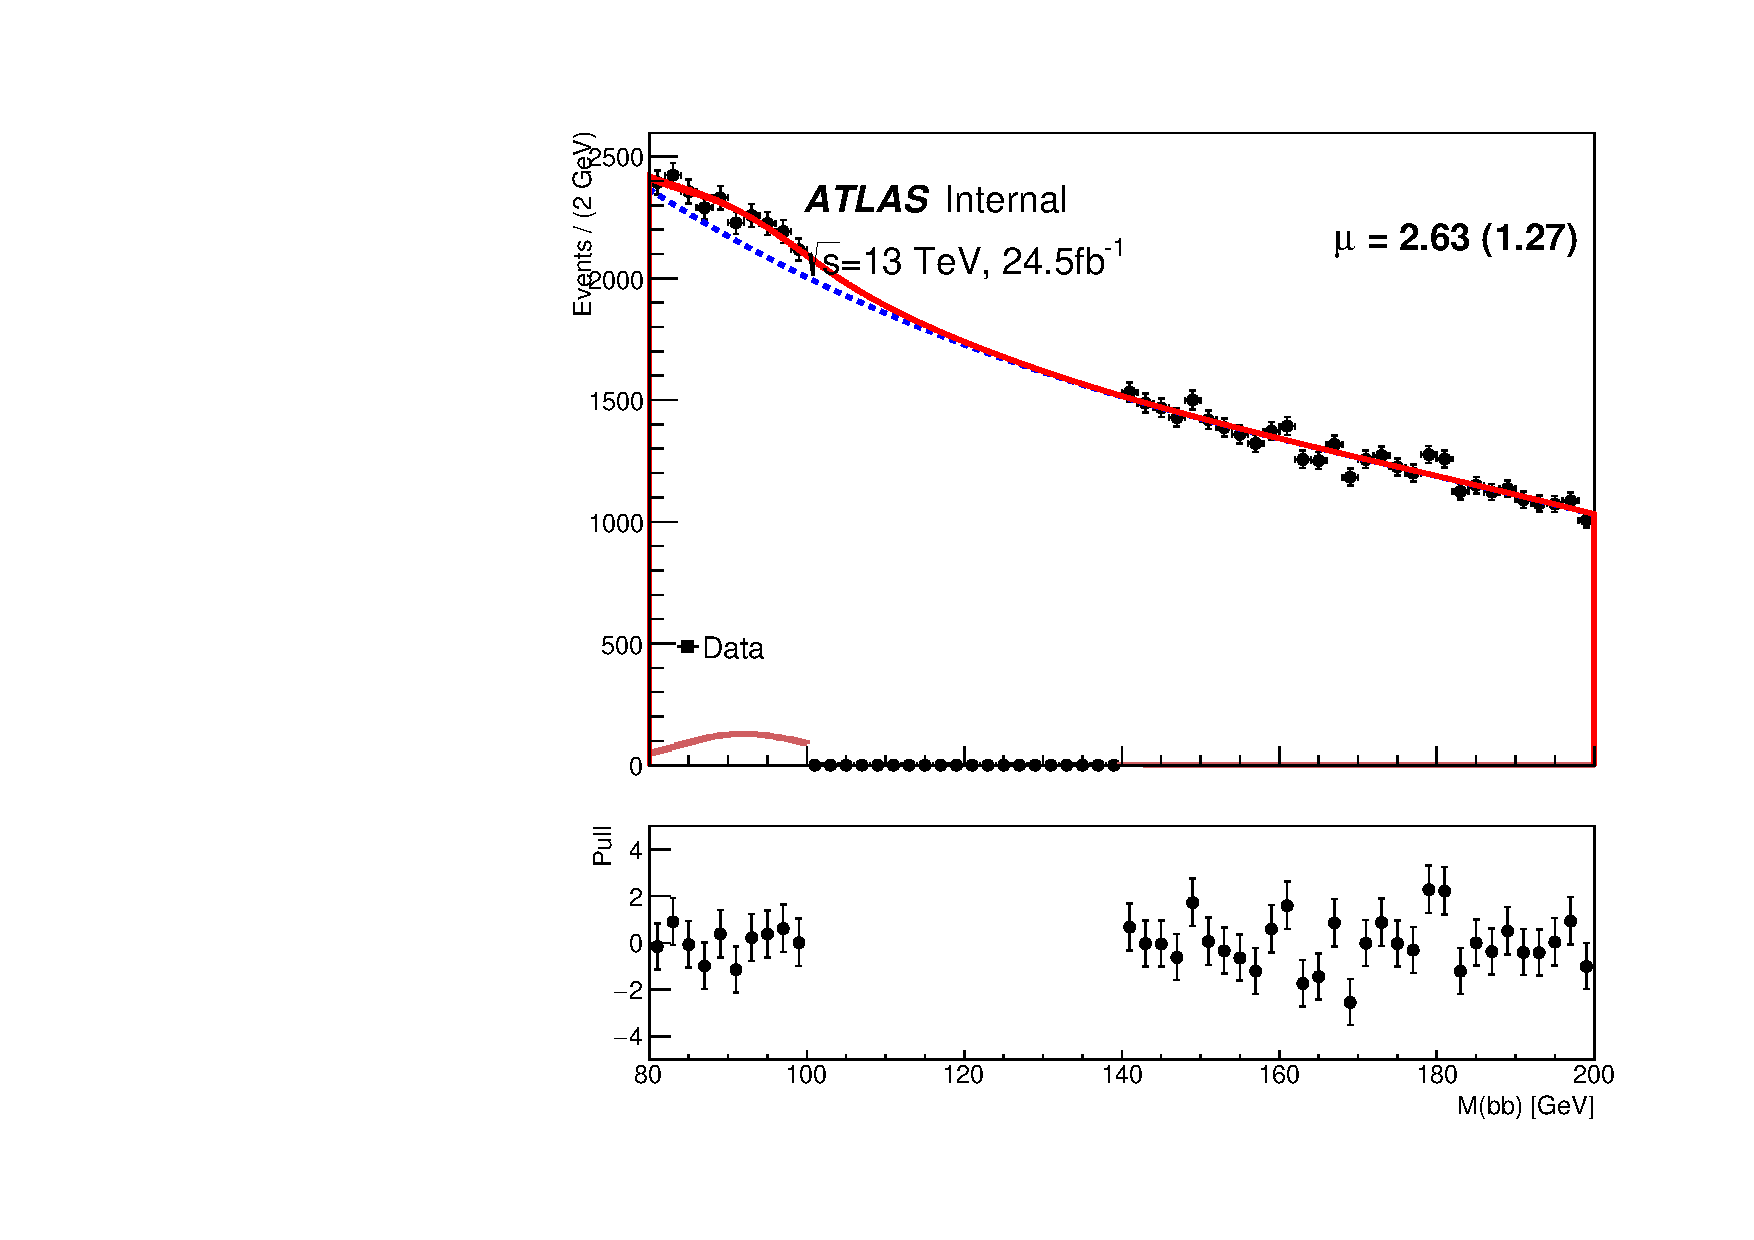
\includegraphics[width=0.24\textwidth]{figures/VBF/zunblind_testVBF_ICHEP_2cen_SRI.pdf}
% 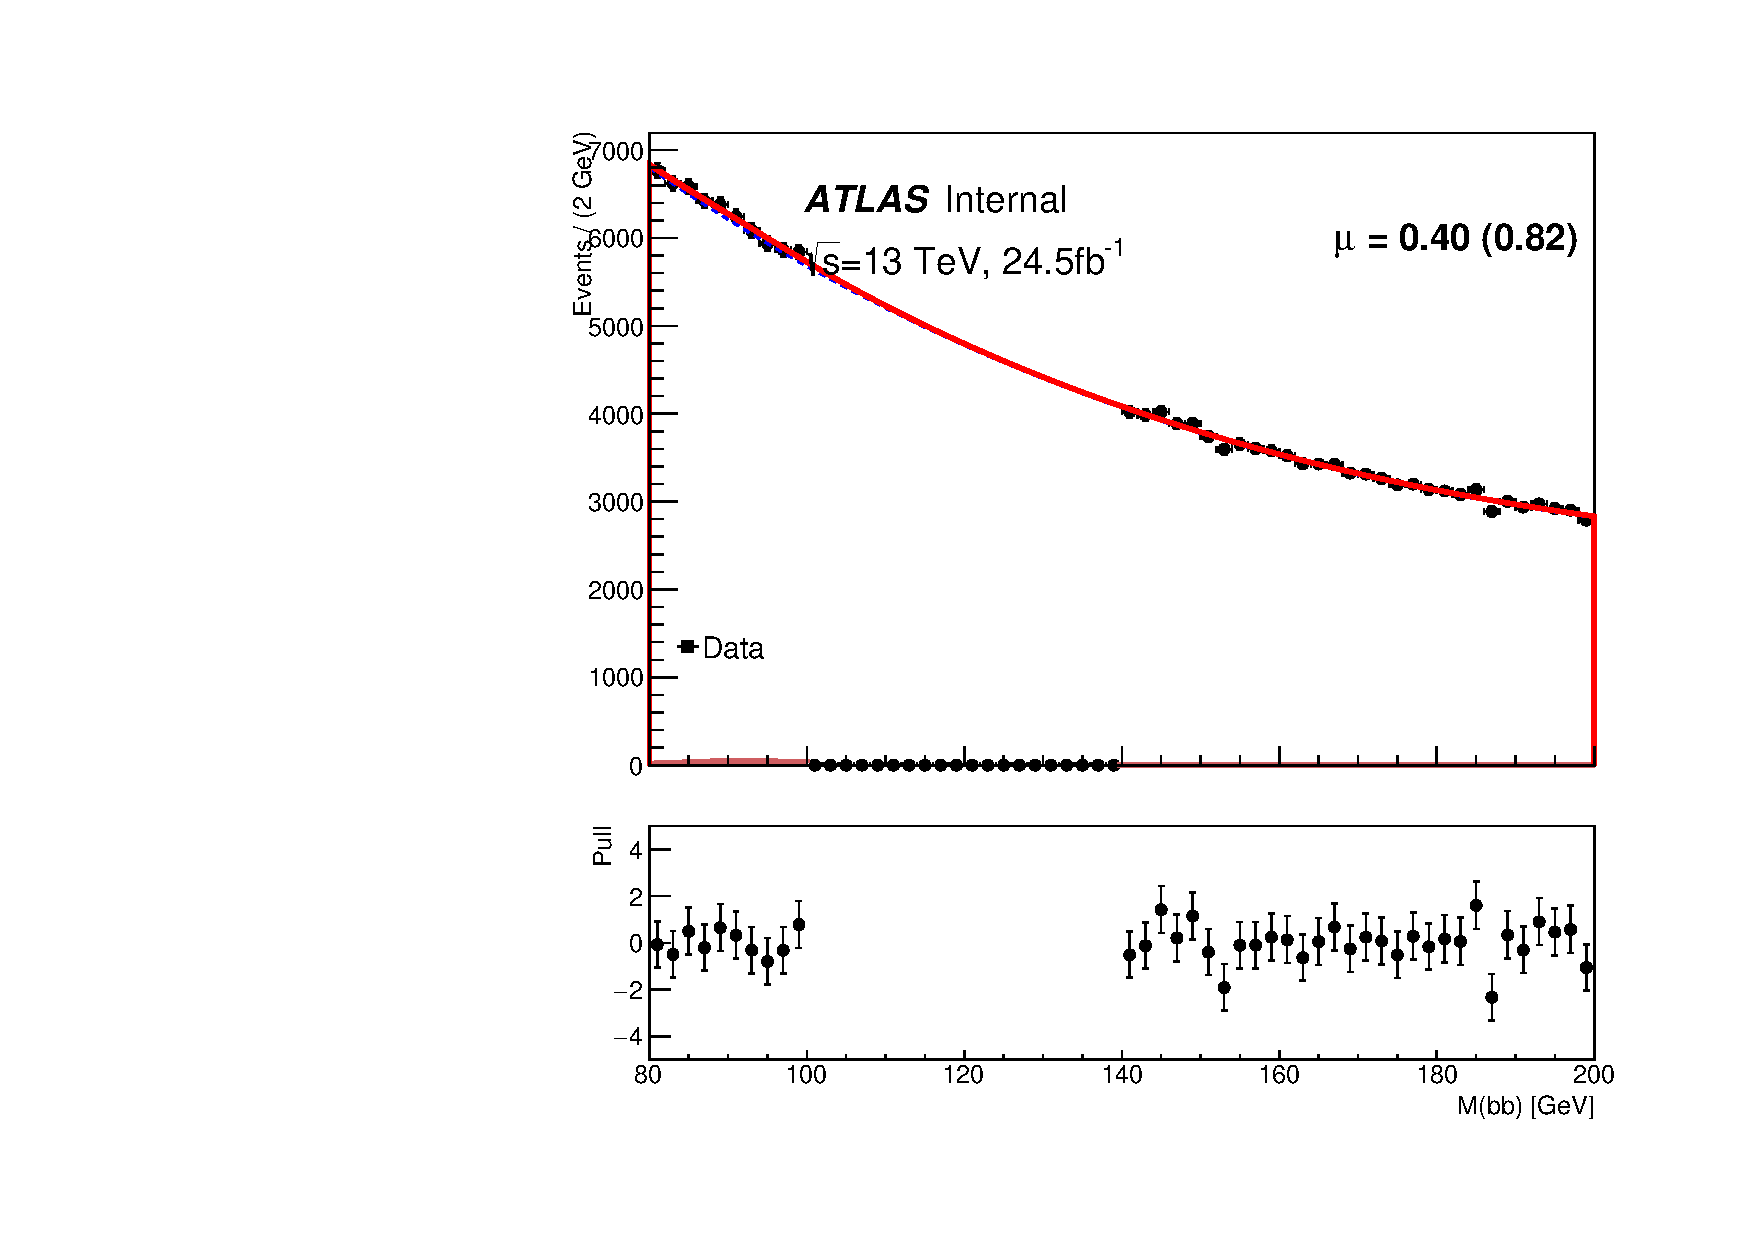
\includegraphics[width=0.24\textwidth]{figures/VBF/zunblind_testVBF_ICHEP_2cen_SRII.pdf}\\
% 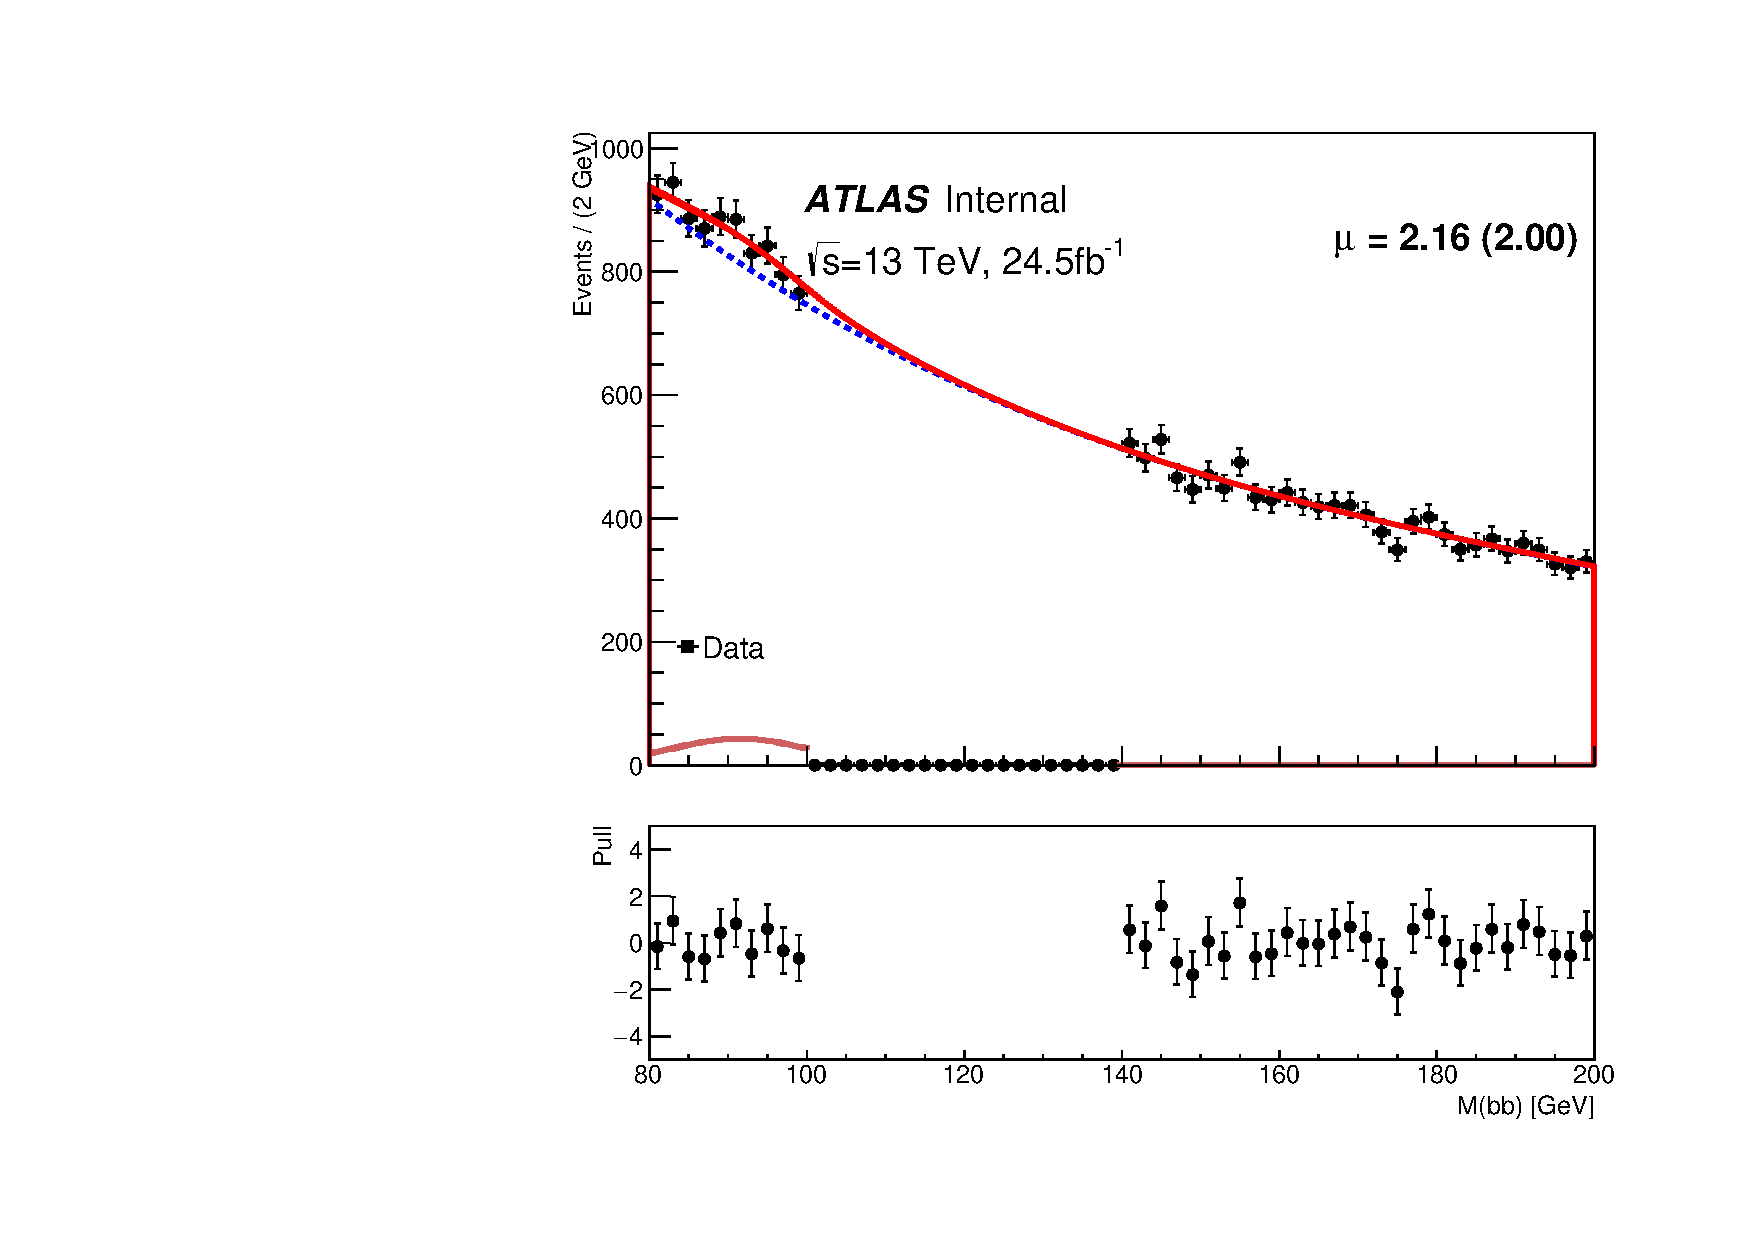
\includegraphics[width=0.24\textwidth]{figures/VBF/zunblind_testVBF_ICHEP_4cen_SRI.pdf}
% 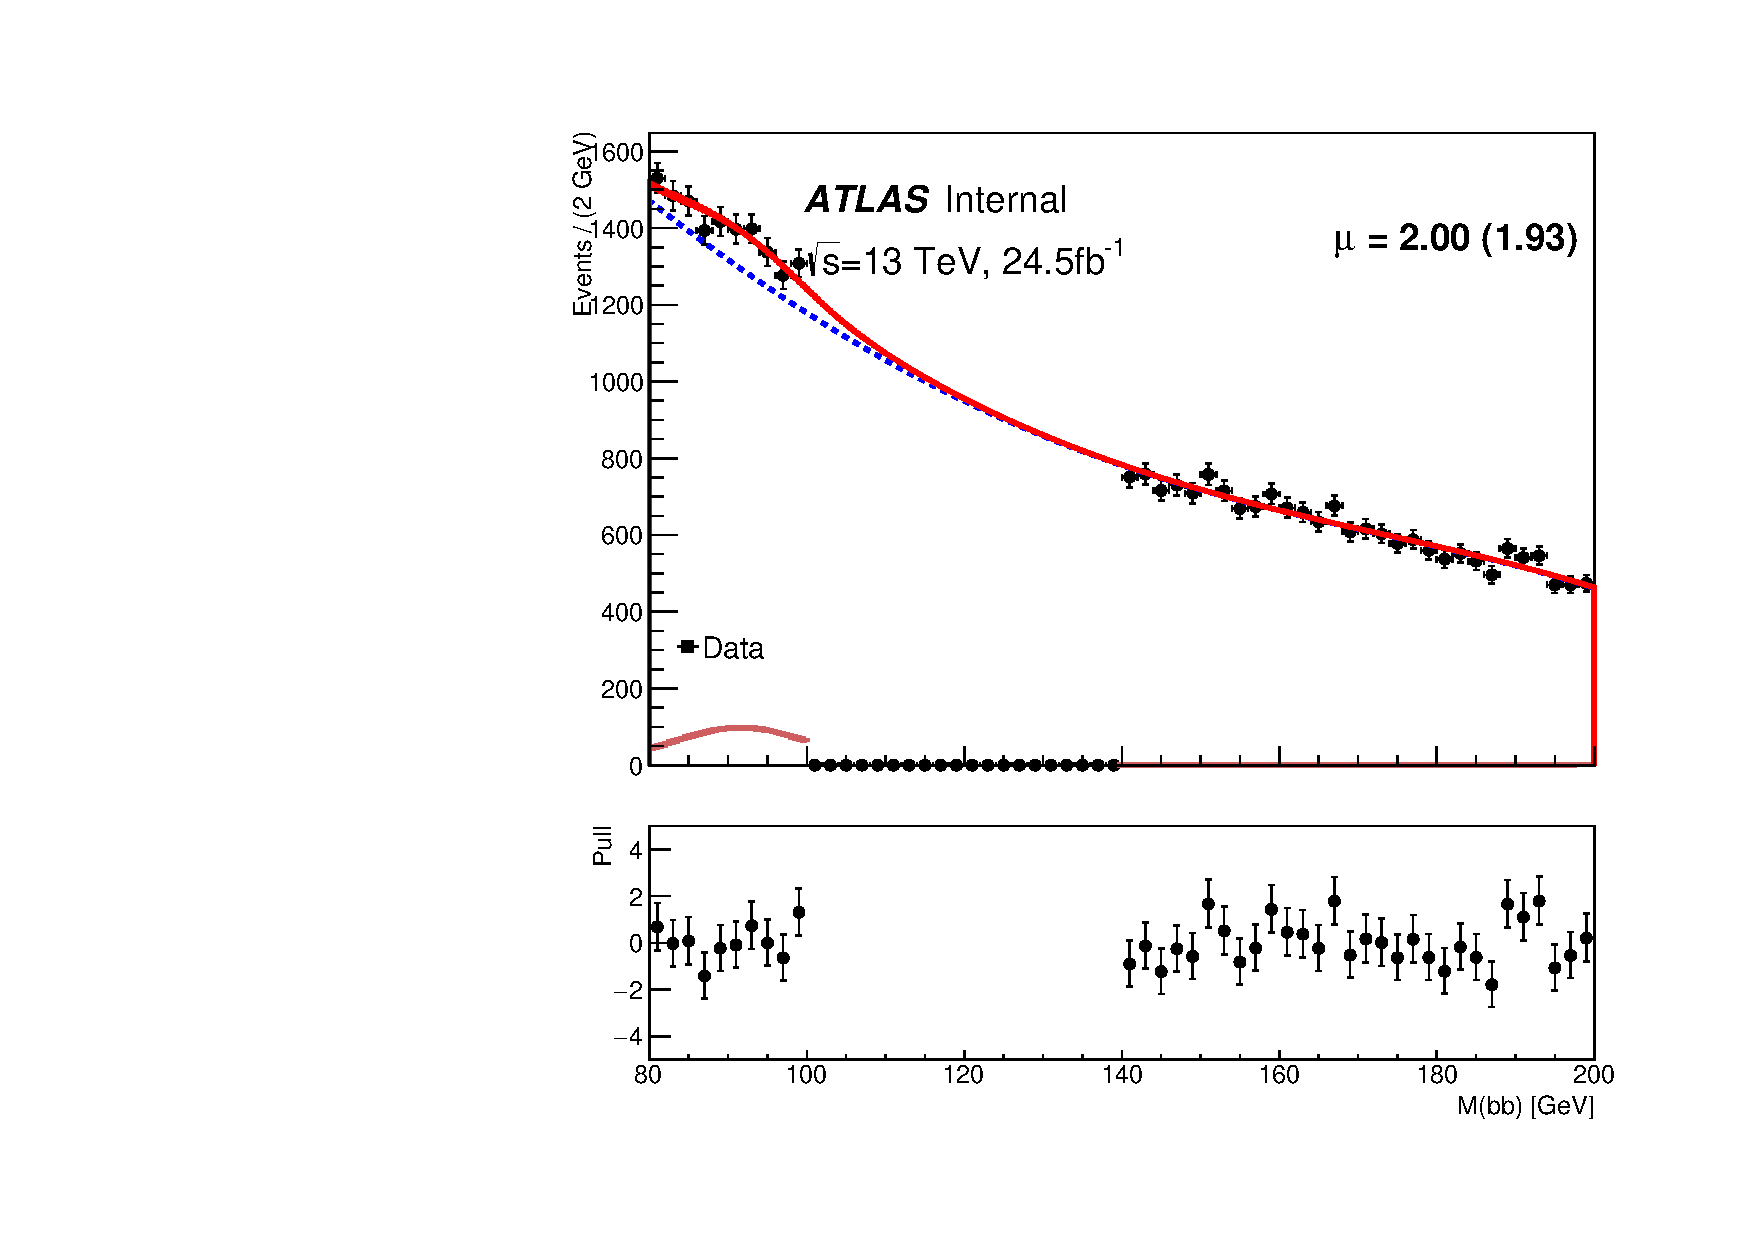
\includegraphics[width=0.24\textwidth]{figures/VBF/zunblind_testVBF_ICHEP_4cen_SRII.pdf}
% 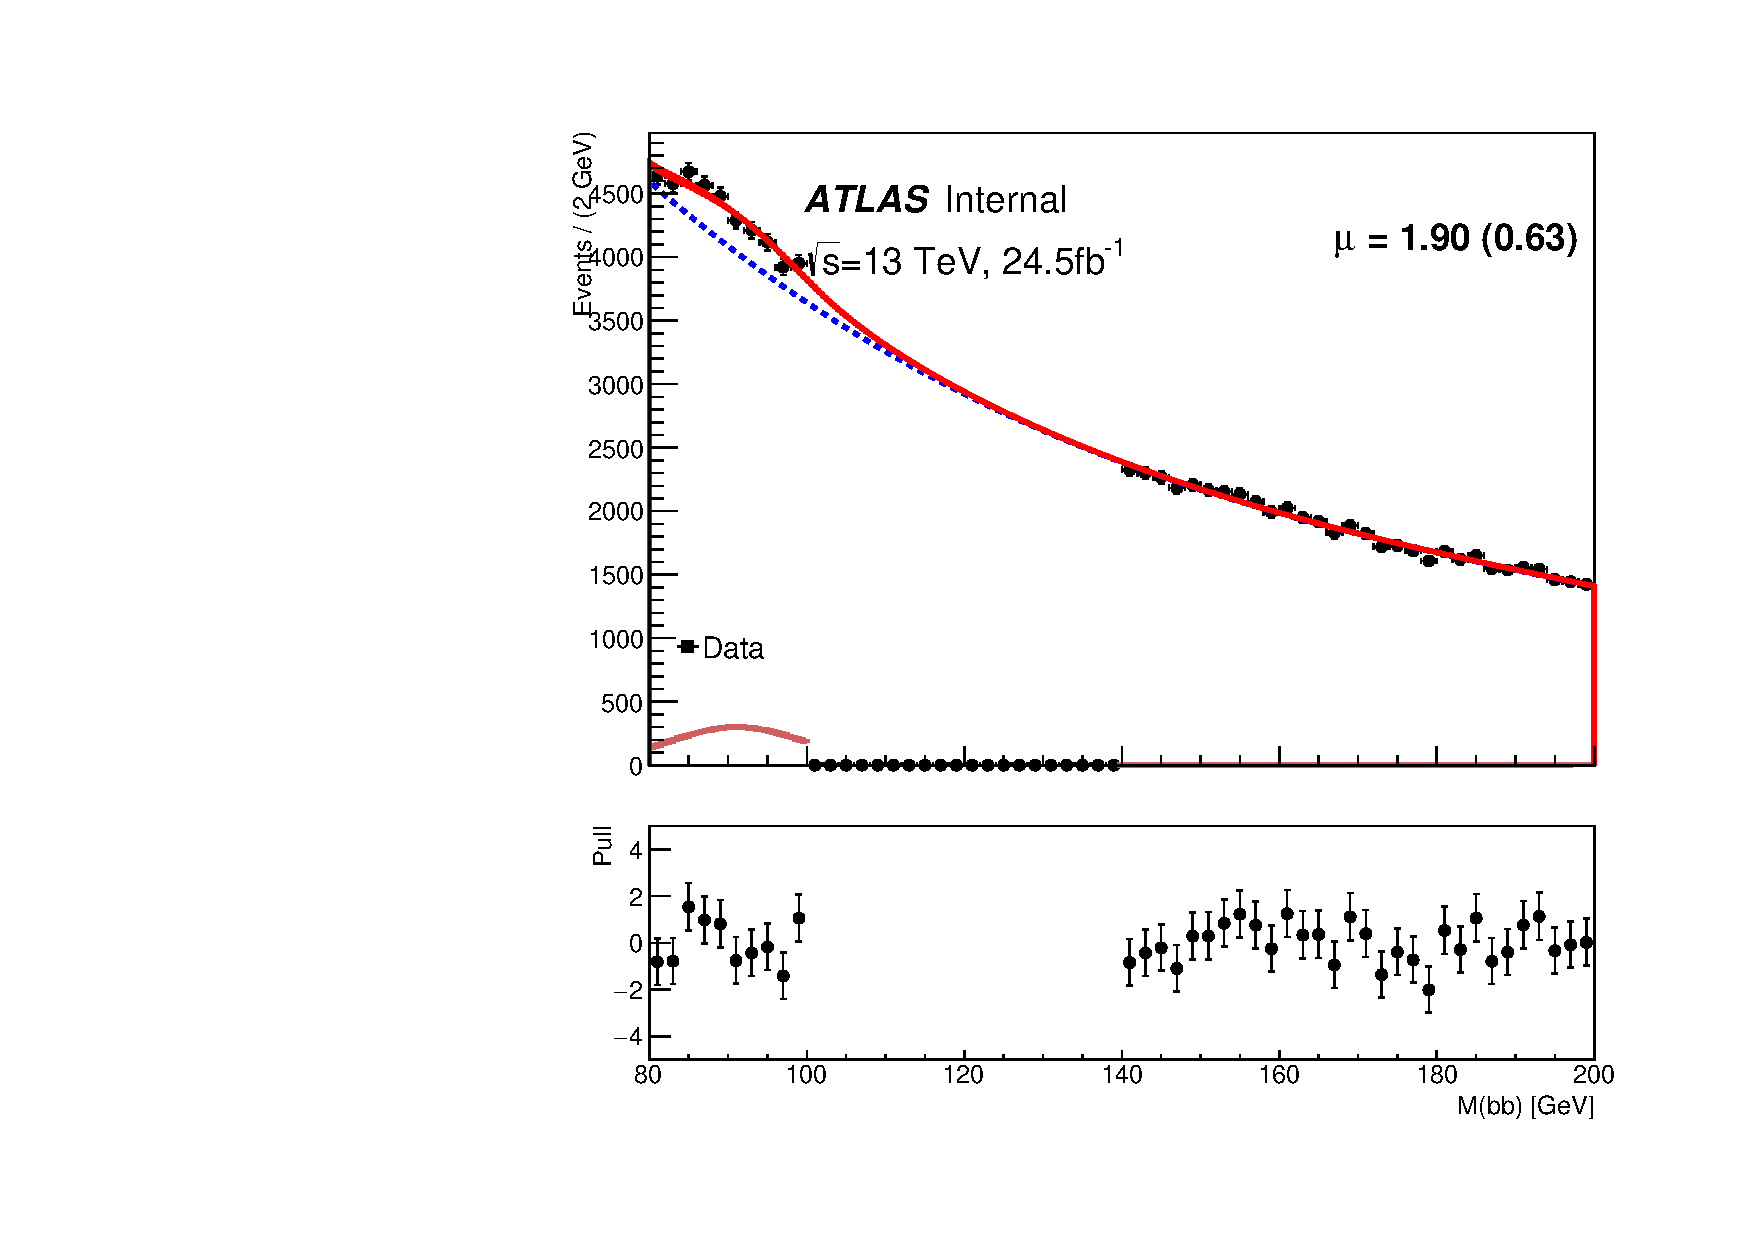
\includegraphics[width=0.24\textwidth]{figures/VBF/zunblind_testVBF_ICHEP_4cen_SRIII.pdf}
% 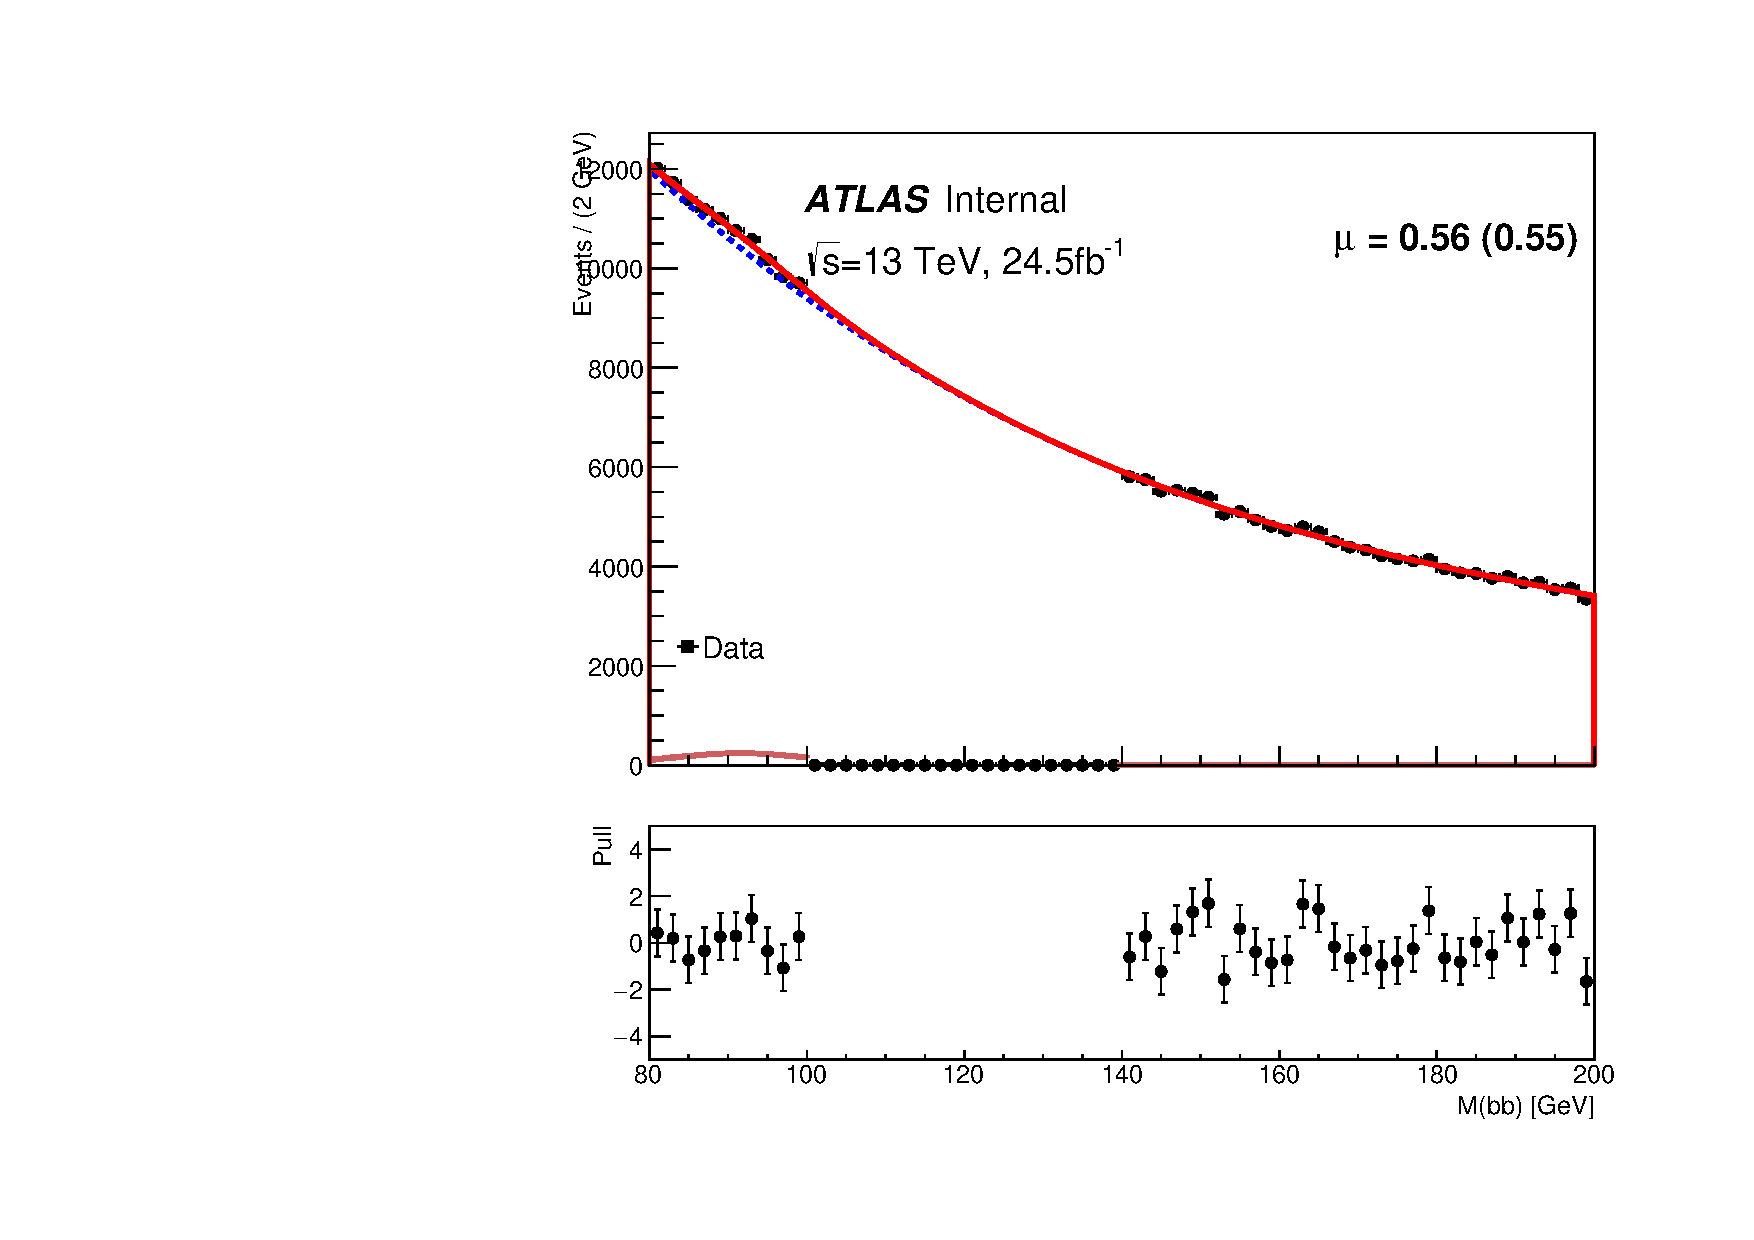
\includegraphics[width=0.24\textwidth]{figures/VBF/zunblind_testVBF_ICHEP_4cen_SRIV.pdf}\\
%\caption{Data and fit model comparison for sideband only \zjets{} fit in \twocentral (top) and \fourcentral channel (bottom) for SR I (left) to SR IV (right).  The data are the black points and the fit model (red), which comprises the continuum background (blue dashed line) and the Z contribution (light red histogram).}
%  \label{fig:vbf-zsidebandfit}
%\end{figure}


\subsection{Extraction of $\mu_{H}$}
\label{sec:vbf-higgsunblind}

The observed value of the Higgs signal strength is $2.7^{+2.2}_{-2.0}$, while the Asimov fit yields $\mu_{H}=1\pm 1.9$. The breakdown of the uncertainty is $\mu_H=2.7^{+1.9}_{-1.9}\textnormal{(stat)}^{+1.1}_{-0.6}\textnormal{(syst)}$ treating the NPs for the analytical background parameterization and normalization as well as the normalization of $Z$ contribution as statistical uncertainty.

%Figures~\ref{fig:vbf-higgsfit_2cen} and ~\ref{fig:vbf-higgsfit_4cen} show the resulting distributions for the \twocentral and \fourcentral channels. %displaying the residuals with respect to the continuum background fit on the bottom panel. % whereas Figures~\ref{fig:vbf-higgsfit_2cen_pull} and~\ref{fig:vbf-higgsfit_4cen_pull} show the pull values with respect to the full background model.  

%The pull values are shown in Figure~\ref{fig:vbf-higgsfitpull} for nuisance parameters with a post-fit impact of more than 4\%.  None of the nuisance parameters are strongly pulled. The largest uncertainty on $\mu_H$ comes from the theory uncertainty on the QCD scale, followed by the background parameterization and the jet energy resolution. The increase of the total uncertainty with respect to the expected value comes from the larger than expected background normalization as well as an increase of the signal systematics which scales as the size of the $\mu_H$. 

The fitted $Z$ values are shown in Table~\ref{tab:zfullfit} for each SR.  Reductions of 30--60\% of the $\mu_Z$ uncertainties are observed with respect to the sideband only fit. A statistical combination of all the channels, as described in Equation~\ref{eqn:zsig}, yields an effective $\mu_Z = 1.2 \pm 0.2$ with a combined $\chi^2/$ndof of 1.05 with a probability of 38.8\%.  

\begin{table}[htbp]
\centering
\caption{Floating Z normalization parameters in full mass range fit.}
\label{tab:zfullfit}
\begin{tabular}{|l|c|c|}
\hline
Channel      & $\mu_{Z}$   & $\chi^2/ndof$ \\ \hline
2 cen SR I   & 2.2$\pm$0.7  & 0.9      \\ \hline
2 cen SR II  & 0.4$\pm$0.4  & 0.7        \\ \hline
4 cen SR I   & 0.3$\pm$1.1  & 0.7         \\ \hline
4 cen SR II  & 1.2$\pm$0.6  & 0.7        \\ \hline
4 cen SR III & 1.4$\pm$0.4  & 0.7         \\ \hline
4 cen SR IV  & 0.9$\pm$0.2  & 0.8          \\ \hline
\end{tabular}
\end{table}


%\begin{figure}[htbp]
%  \centering
% 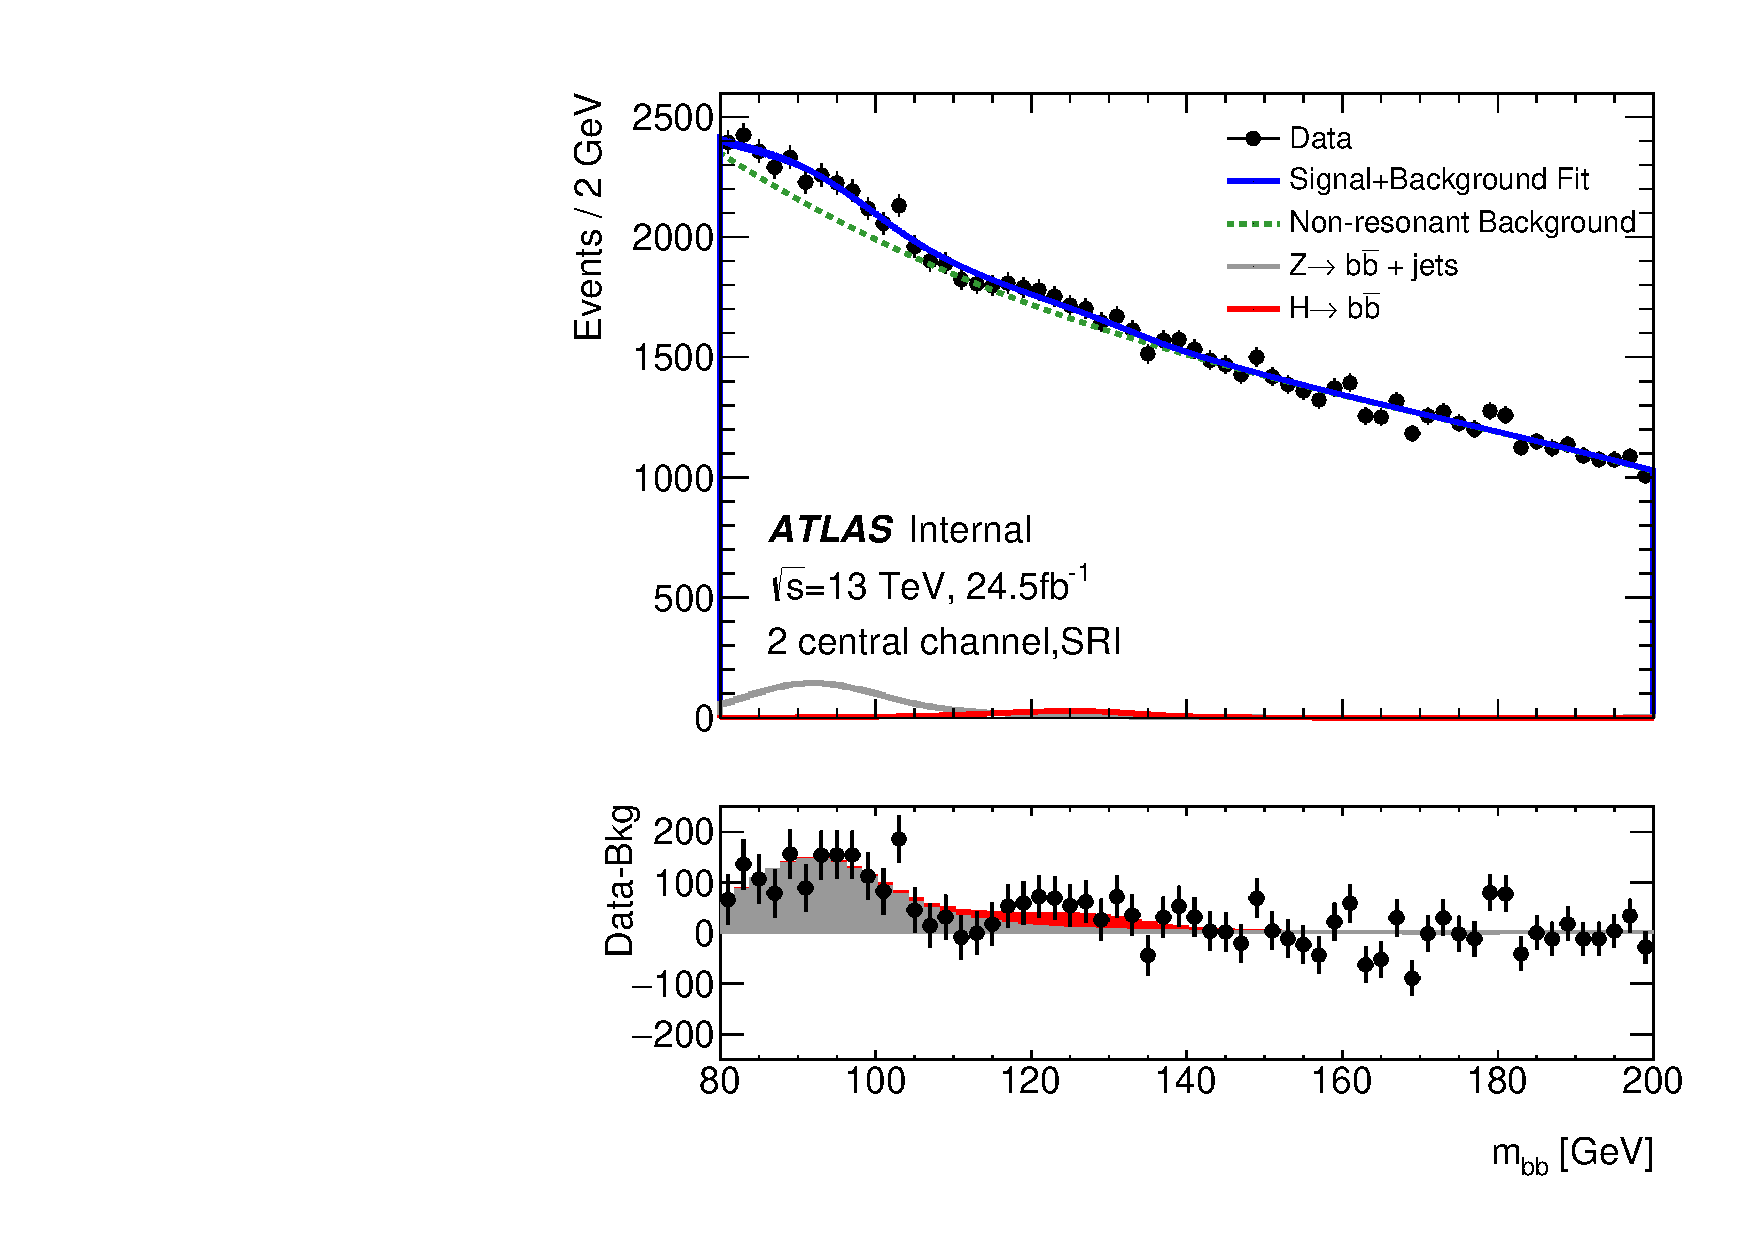
\includegraphics[width=0.48\textwidth]{figures/VBF/unblind_testVBF_ICHEP_2cen_SRI.pdf}
% 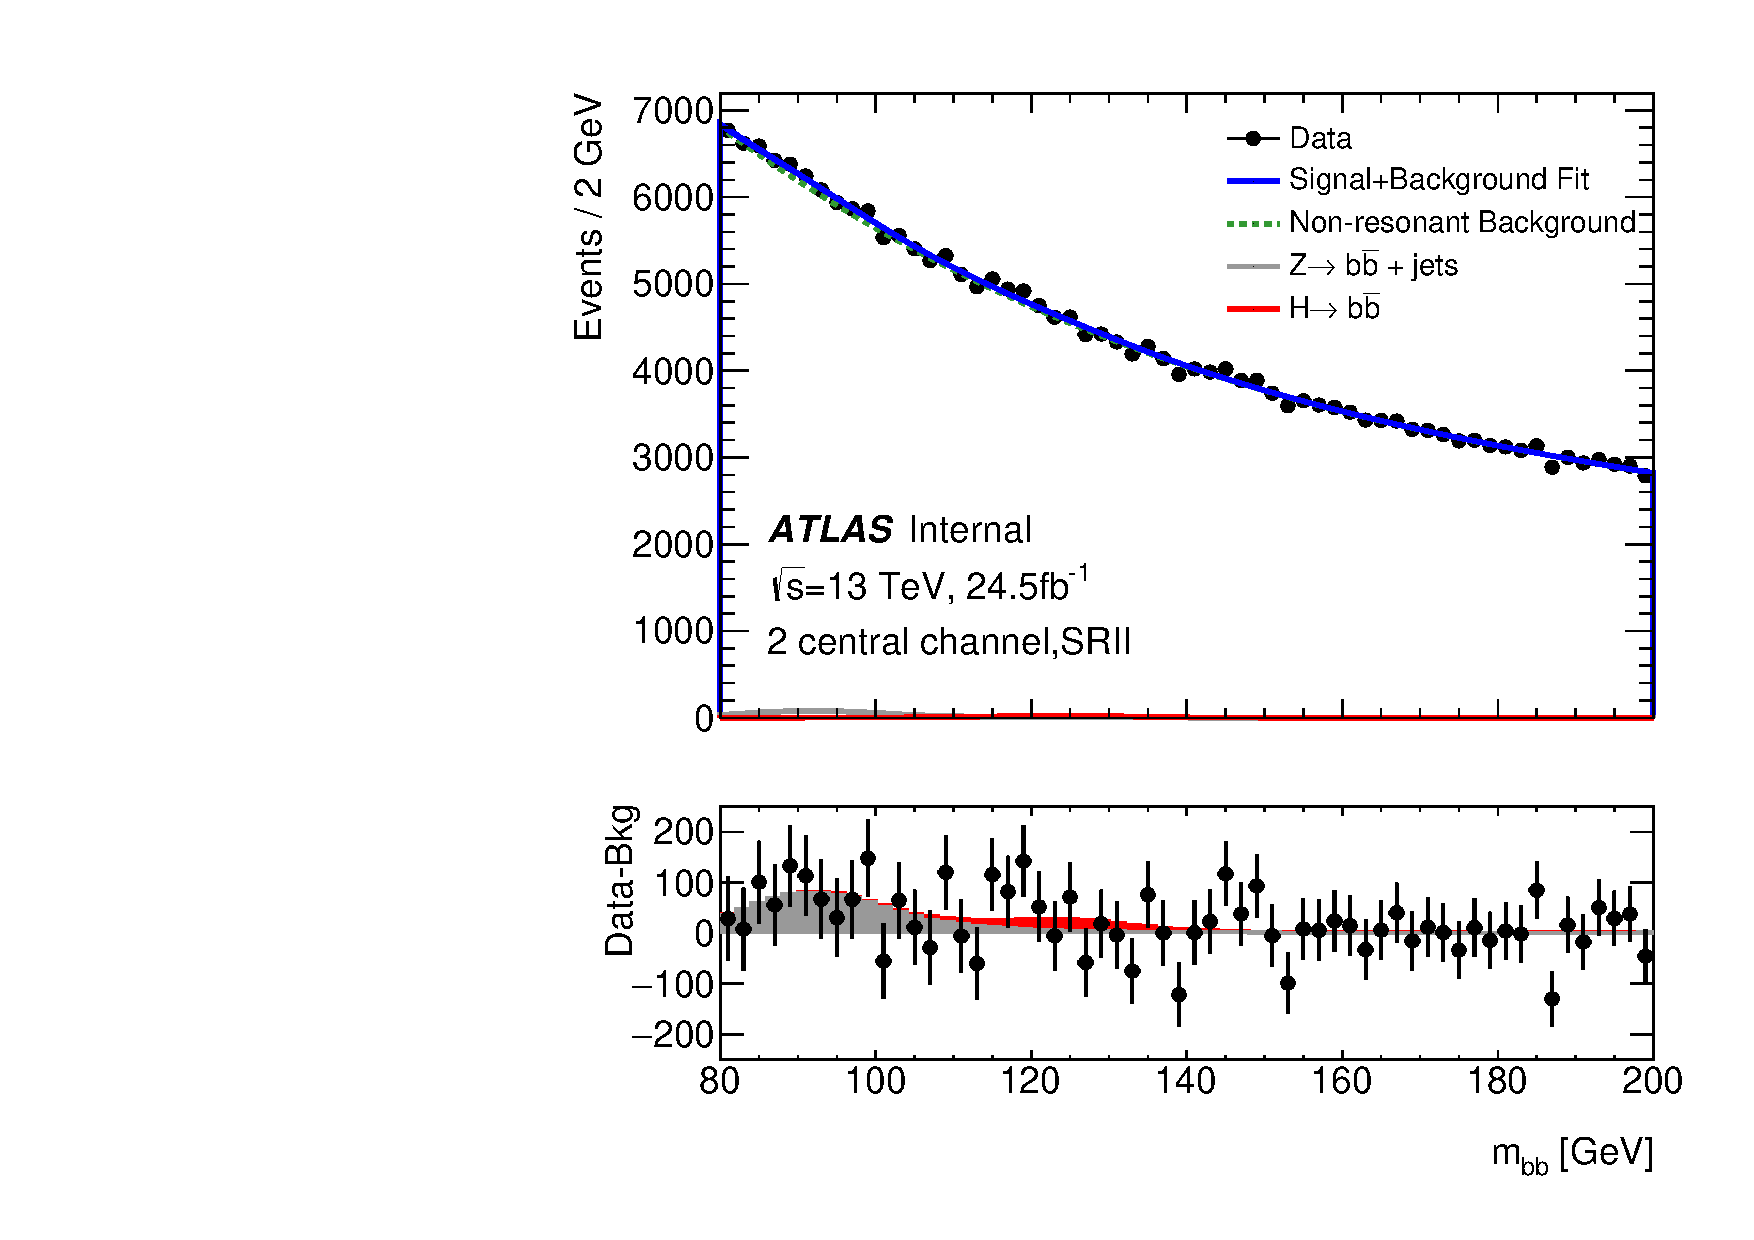
\includegraphics[width=0.48\textwidth]{figures/VBF/unblind_testVBF_ICHEP_2cen_SRII.pdf}\\
%\caption{Data and fit model comparison for profile likelihood fit in the \twocentral channel signal regions.  The fitted continuum background is shown with at  dashed green line, the fitted $Z$ signal in green, and the fitted Higgs signal in red.  The total fit is displayed as the blue line.  The bottom panels show the residual of the data with respect to the continuum background fit, and the fitted $Z$ signal (grey) and Higgs signal (red) are also displayed. }
%  \label{fig:vbf-higgsfit_2cen}
%\end{figure}
%
%\begin{figure}[htbp]
%  \centering
% 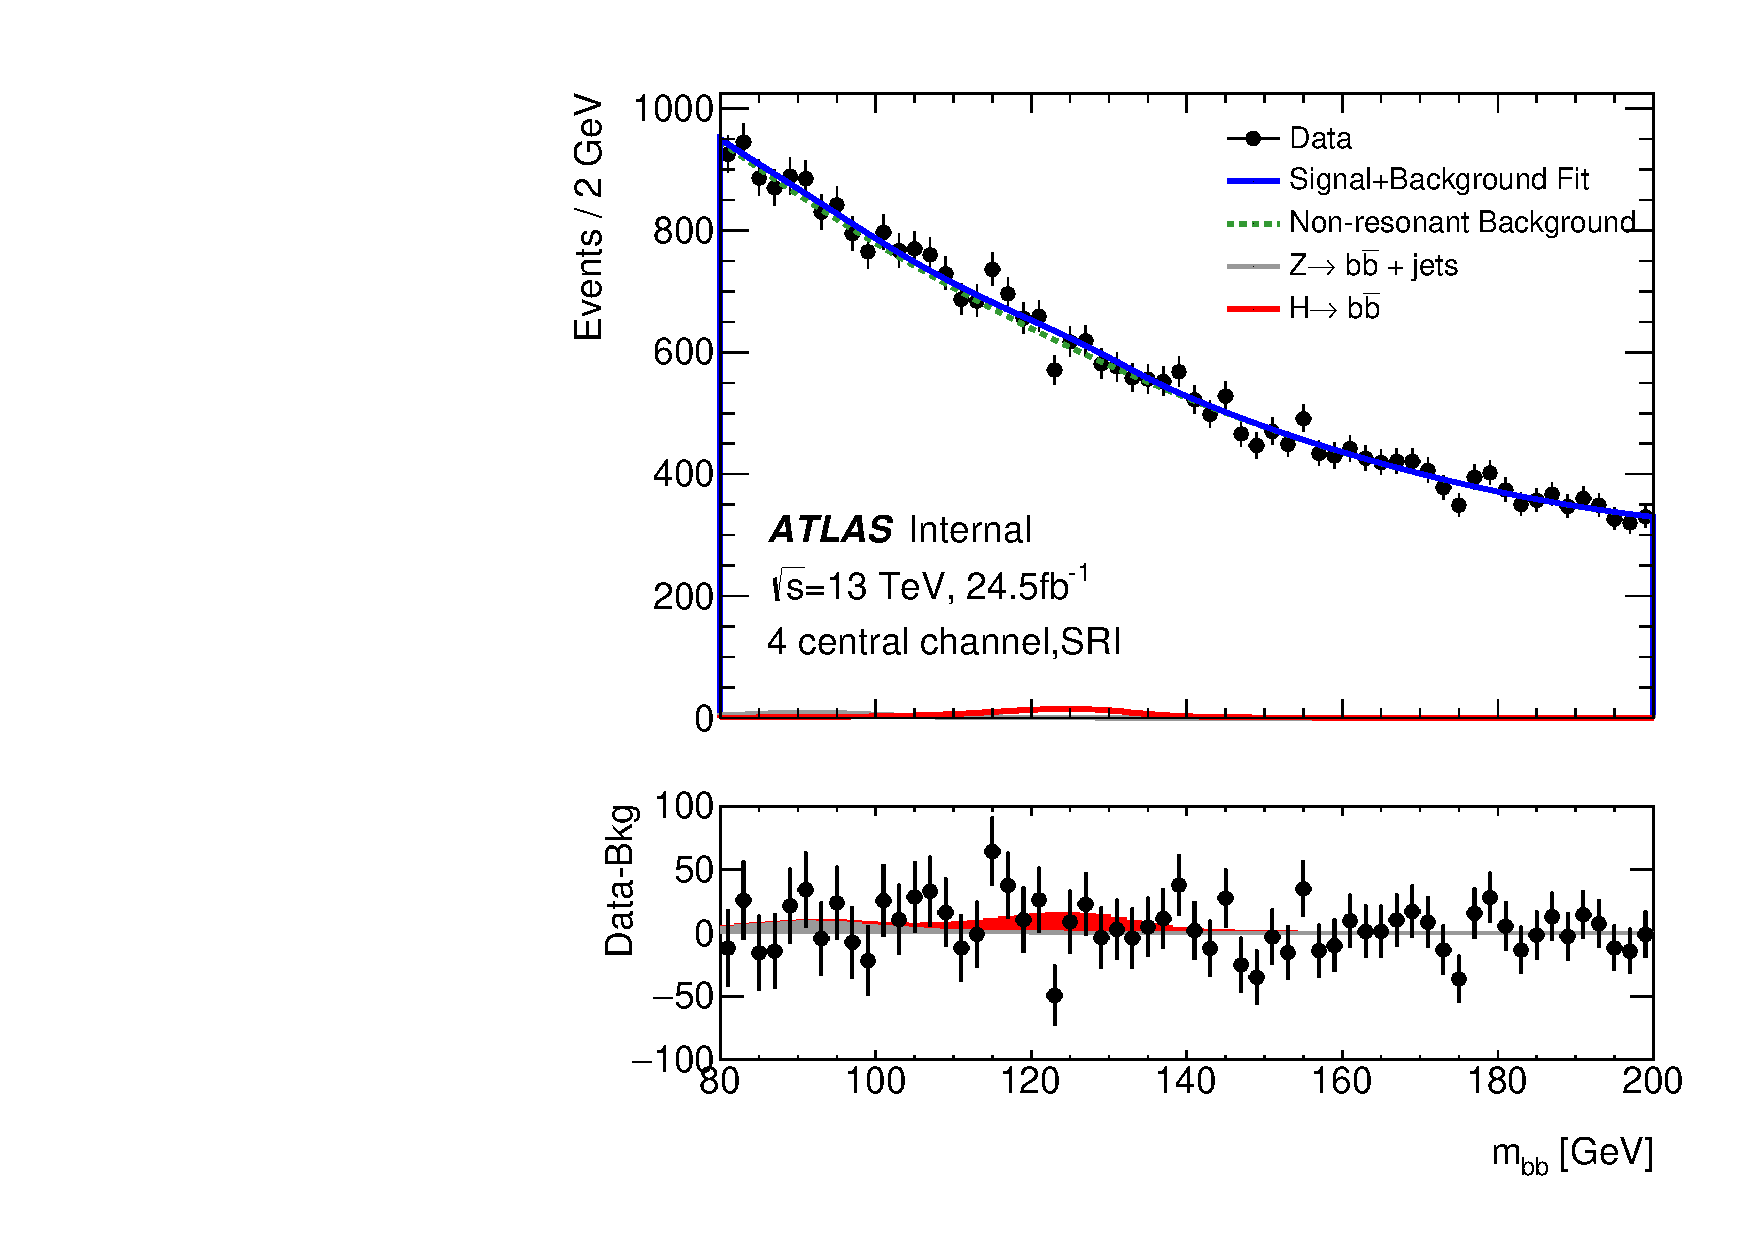
\includegraphics[width=0.48\textwidth]{figures/VBF/unblind_testVBF_ICHEP_4cen_SRI.pdf}
% 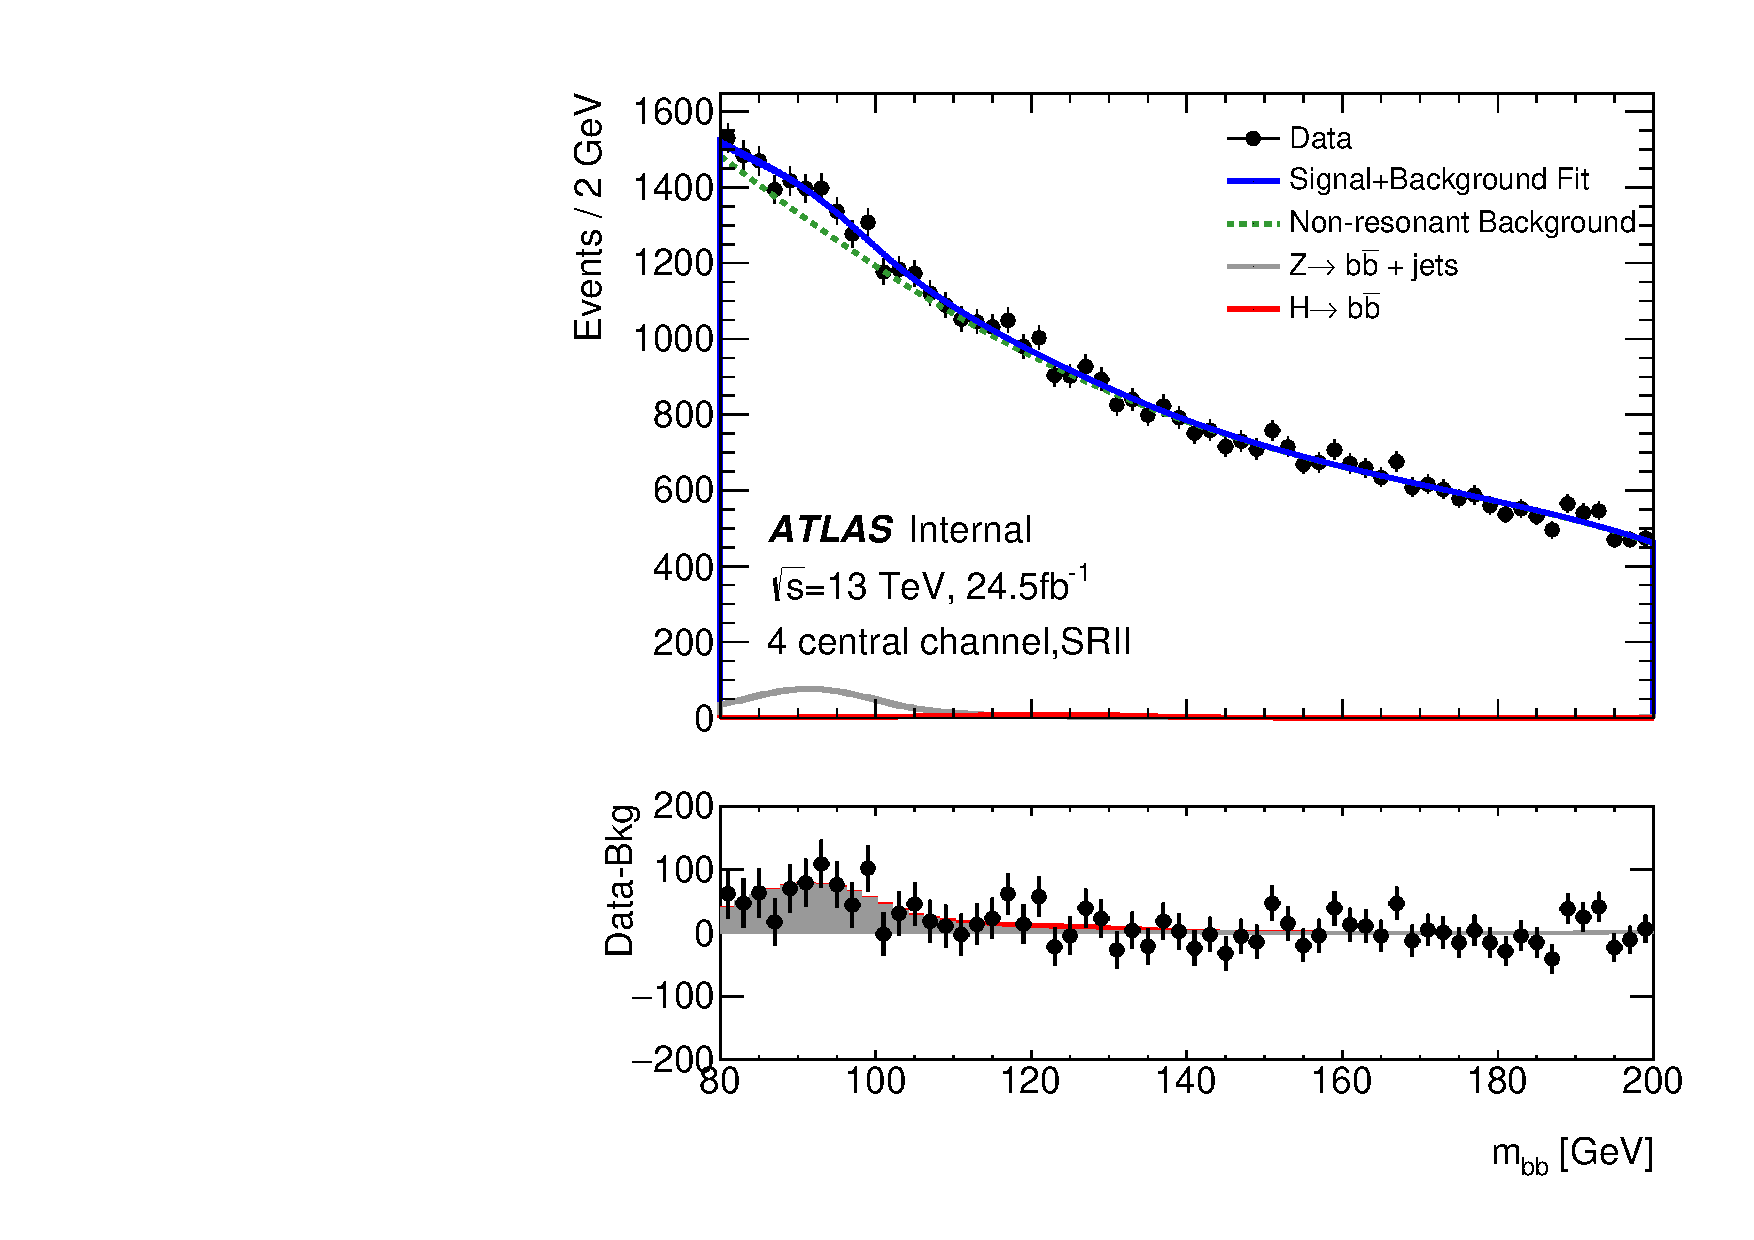
\includegraphics[width=0.48\textwidth]{figures/VBF/unblind_testVBF_ICHEP_4cen_SRII.pdf}\\
% 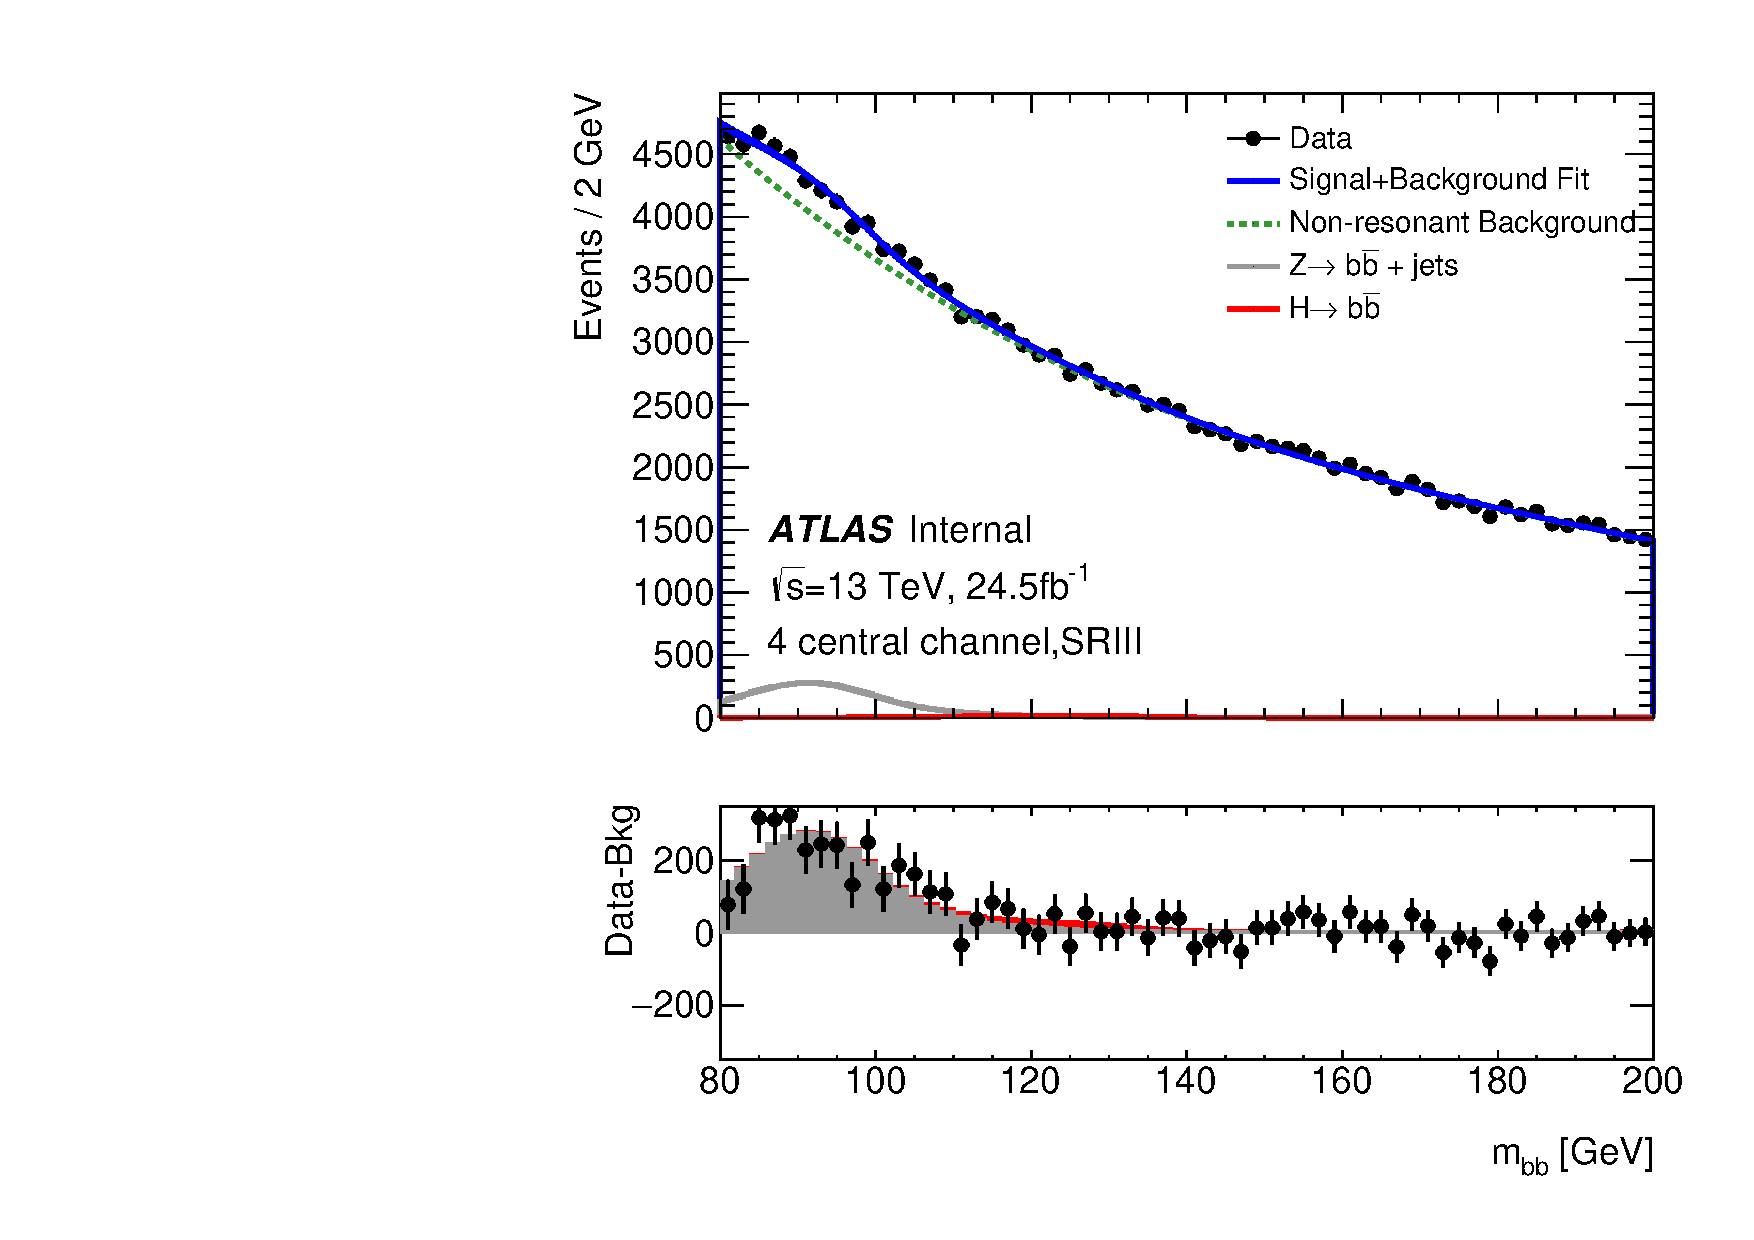
\includegraphics[width=0.48\textwidth]{figures/VBF/unblind_testVBF_ICHEP_4cen_SRIII.pdf}
% 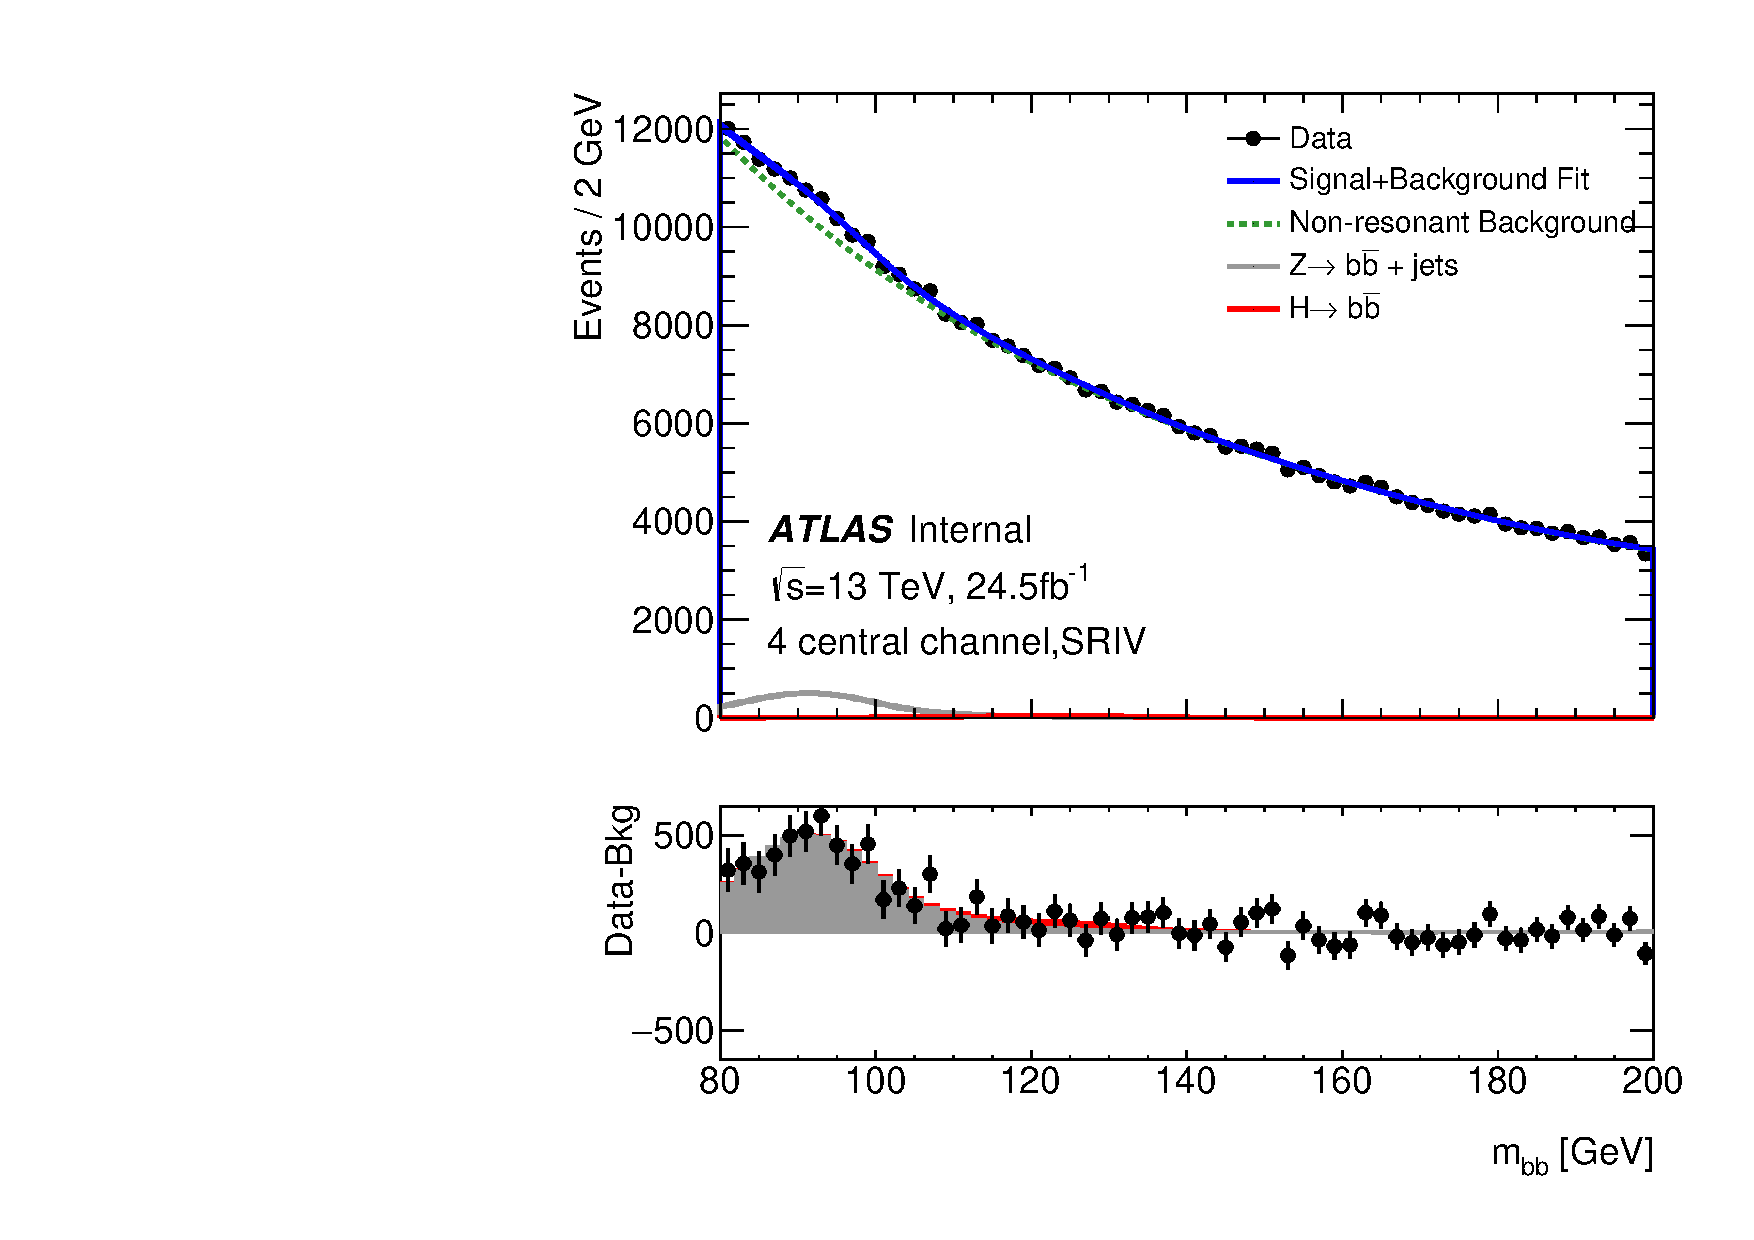
\includegraphics[width=0.48\textwidth]{figures/VBF/unblind_testVBF_ICHEP_4cen_SRIV.pdf}\\
%\caption{Data and fit model comparison for profile likelihood fit in the \fourcentral channel signal regions. The fitted continuum background is shown with at  dashed green line, the fitted $Z$ signal in green, and the fitted Higgs signal in red.  The total fit is displayed as the blue line.  The bottom panels show the residual of the data with respect to the continuum background fit, and the fitted $Z$ signal (grey) and Higgs signal (red) are also displayed.}
%  \label{fig:vbf-higgsfit_4cen}
%\end{figure}


\subsection{Extraction of $\mu_{VBF}$}
\label{sec:vbf-higgsunblindvbf}
A different interpretation of the analysis is the extraction of $\mu_{VBF}$ signal strength.
The fit procedure follows the same way as the extraction of $\mu_{H}$, except we only float
the $VBF$ signal in the fit while fixing the yield of all other Higgs modes, i.e. ggF,
ttH and VH to their Standard Model predictions (with uncertainties applied).
The Asimov fit yields $\mu_{VBF}=1\pm 2.8$. The unblinded value of the VBF Higgs signal
strength is $4.1^{+3.2}_{-2.9}$. The breakdown of the uncertainty
is $\mu_{VBF}=4.1^{+2.8}_{-2.8}\textnormal{(stat)}^{+1.5}_{-0.8}\textnormal{(syst)}$ treating
the NPs for the analytical background parameterization and normalization as well as
the normalization of $Z$ contribution as statistical uncertainty.


\subsubsection{Combination with VBF$+\gamma$ Analysis}
\label{sec:vbf-higgscomb}

The combination of the all-hadronic VBF analysis and the
VBF$+\gamma$ analysis~\cite{vbfplusgammaint} is performed
by a simultaneous likelihood fit to both datasets. The Higgs signal strength is
treated as correlated across all analysis regions,
the $Z$ contributions are extracted as described in the respective analyses.
As described in Section~\ref{sec:vbf-presel}, overlap between the two samples is removed.

The combined fit yields $\mu_H = 2.5^{+1.4}_{-1.3}$ corresponding to an observed significance
of $1.9\sigma$ ($0.8\sigma$ expected). The $VBF$ signal only extraction is also performed combining two analyses similar to \ref{sec:vbf-higgsunblindvbf}. The combined fit yields $\mu_{VBF} =3.0^{+1.7}_{-1.6}$ corresponding to an observed significance of $1.9\sigma$ ($0.7\sigma$ expected). The data and fit model comparisons for $\mu_{VBF}$ extraction are shown in Fig.\ref{fig:higgsfit_2cen},\ref{fig:higgsfit_4cen},\ref{fig:mbb_postfit_photon}.

The extractions of $\mu_{H}$ and $\mu_{VBF}$ for separate fits of both all-hadronic and photon analysis and the combination fit are summarized in Fig.\ref{fig:vbf-summary}.


\begin{figure}[htbp]
  \centering
 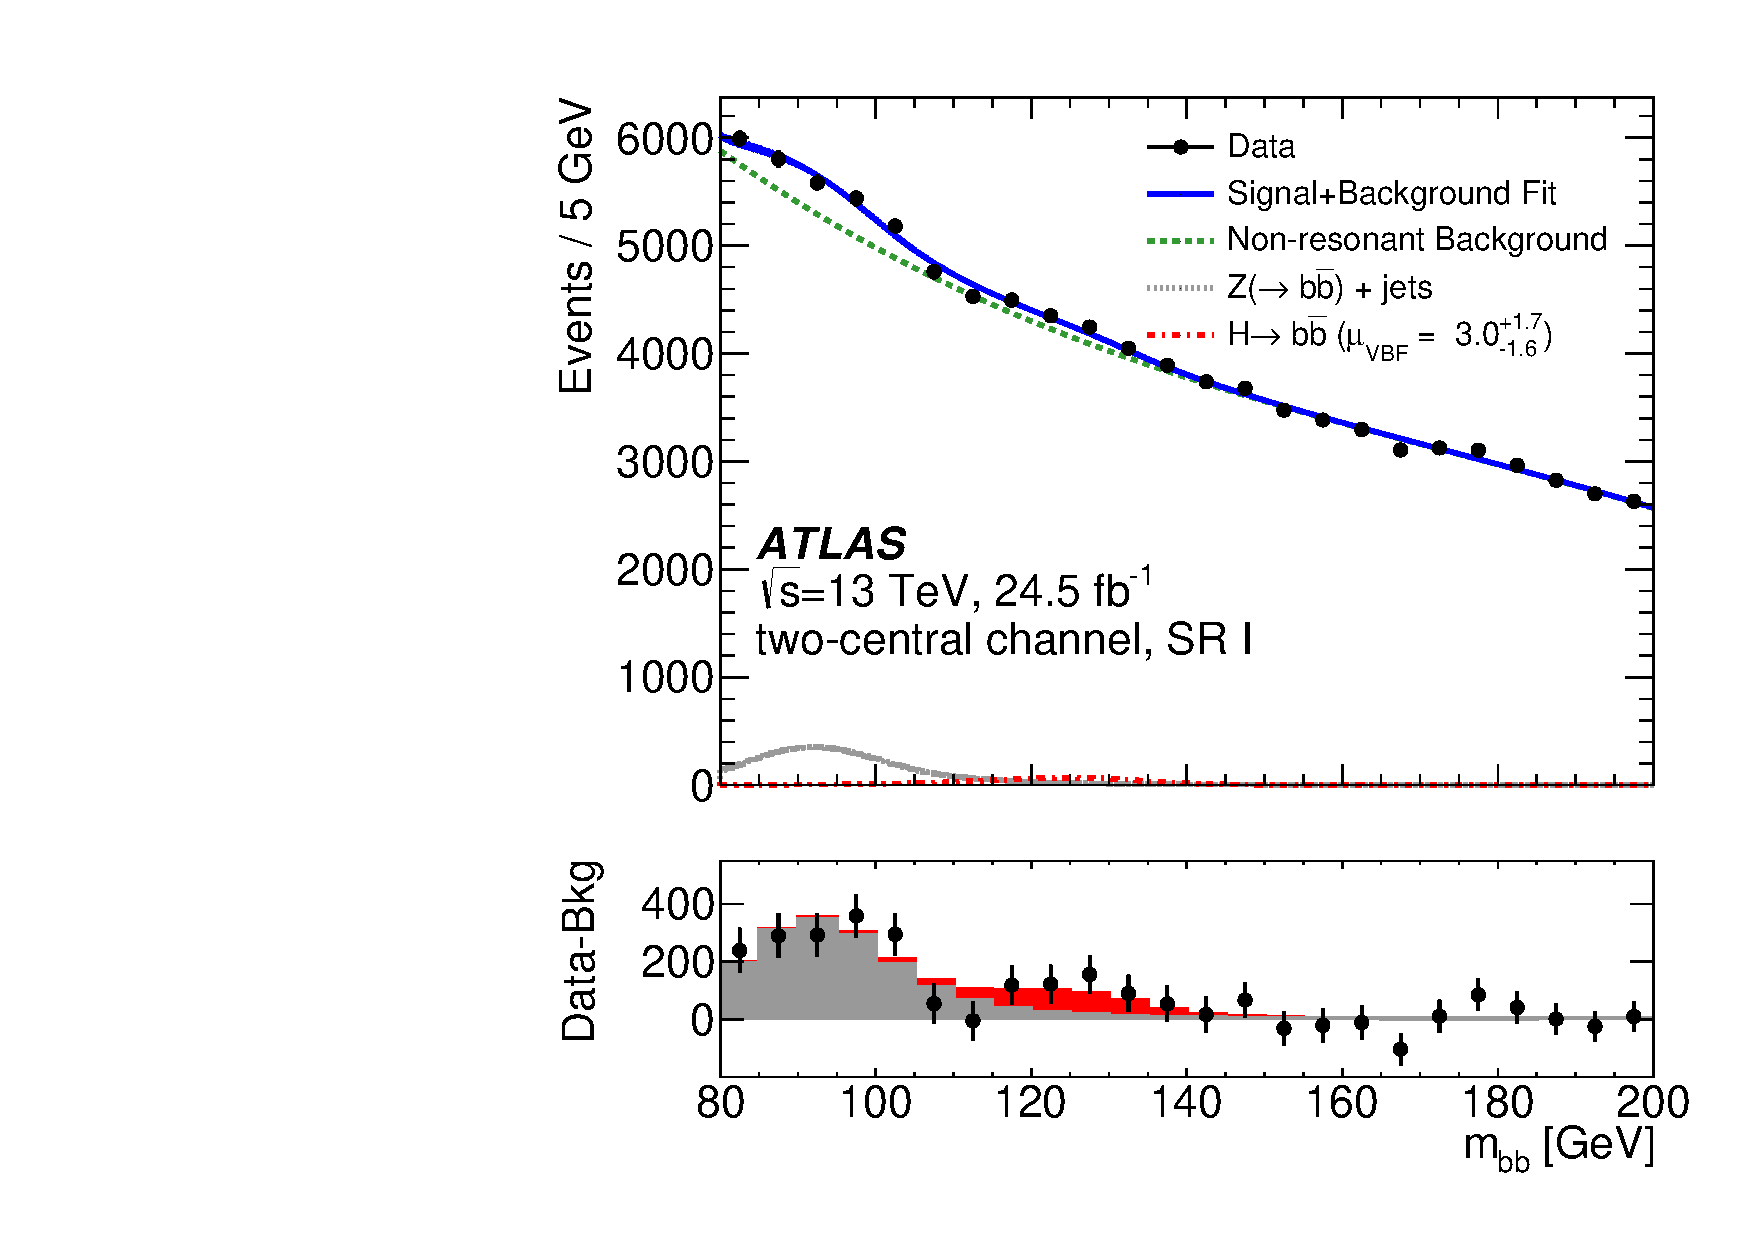
\includegraphics[width=0.48\textwidth]{figures/VBF/comb_vbfonly_testVBF_ICHEP_2cen_SRI_vbfincl.pdf}
 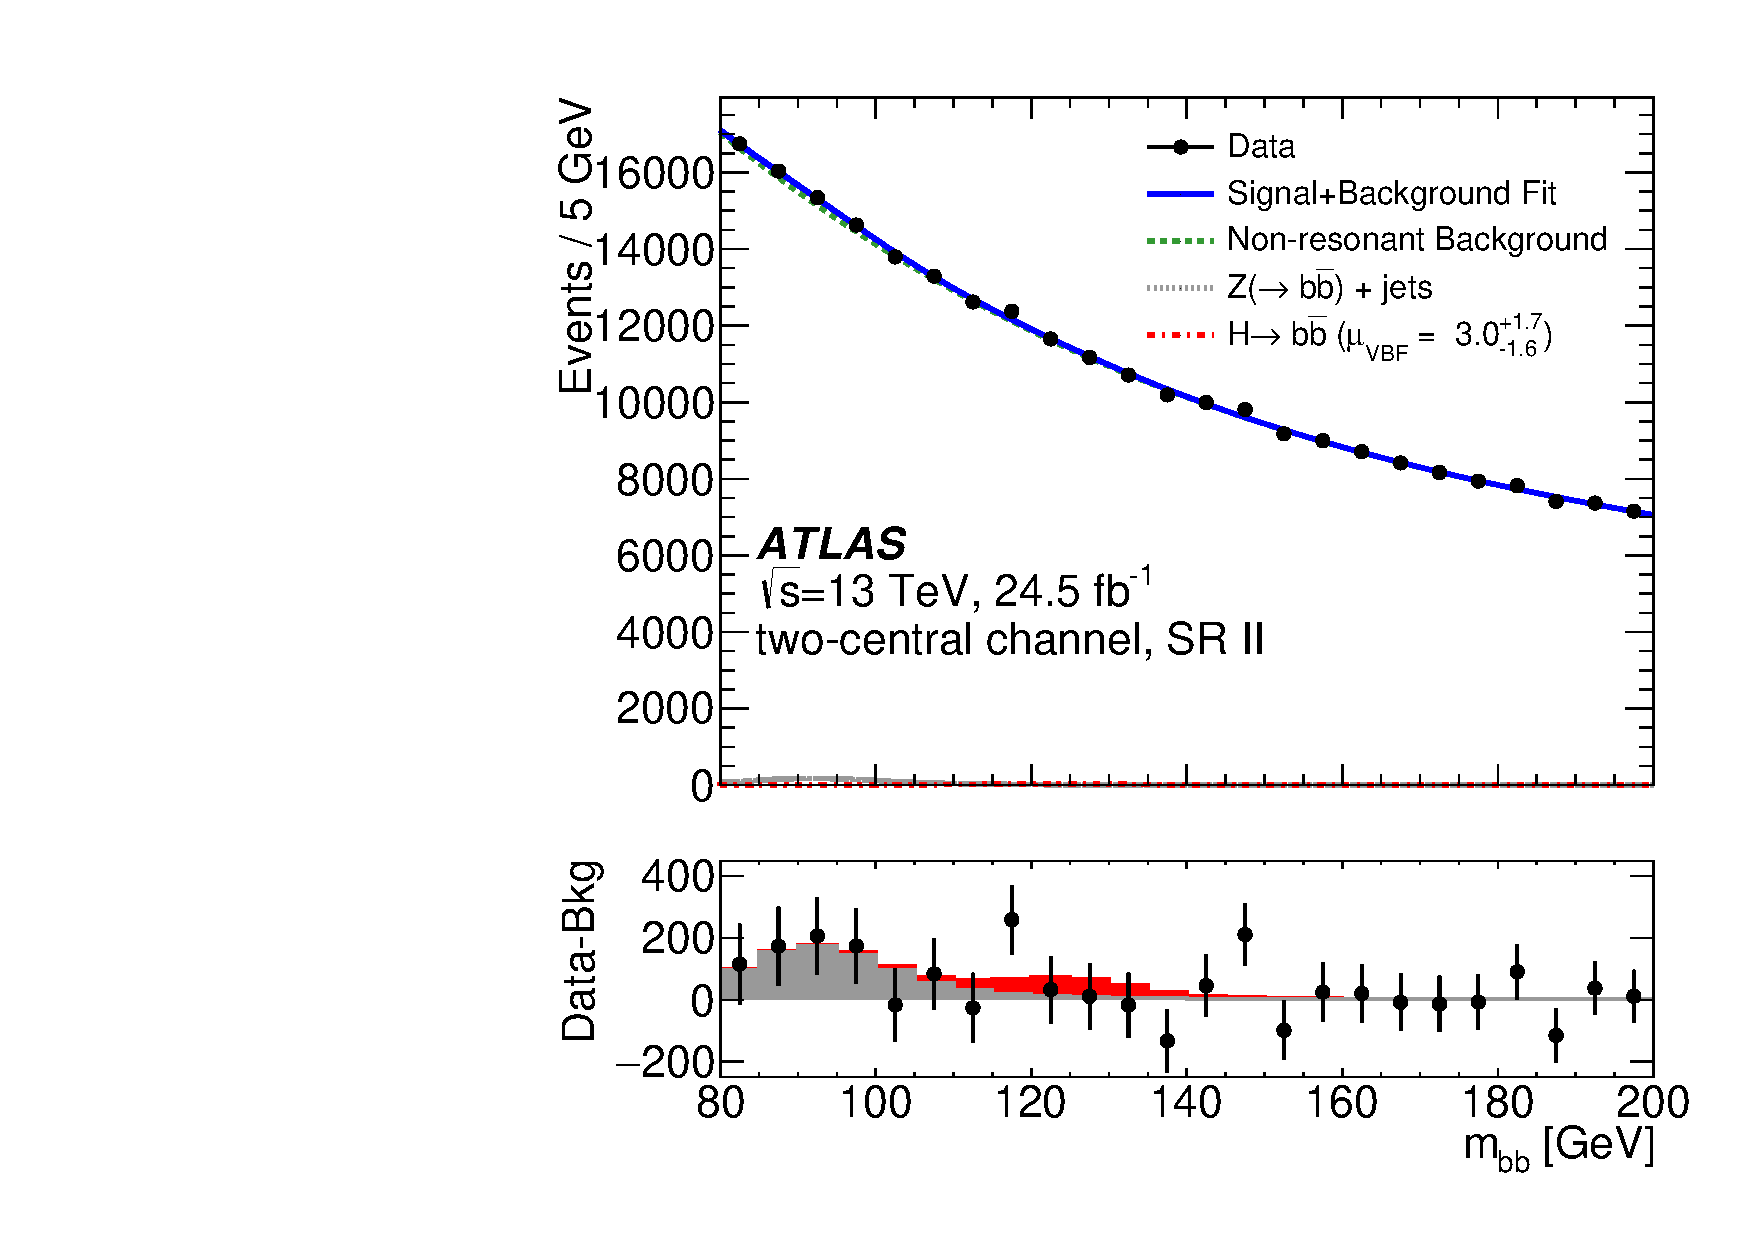
\includegraphics[width=0.48\textwidth]{figures/VBF/comb_vbfonly_testVBF_ICHEP_2cen_SRII_vbfincl.pdf}\\

\caption{Data and fit model comparison for the combined fit of $\mu_{VBF}$ extraction in the \twocentral channel}
  \label{fig:higgsfit_2cen}
\end{figure}

\begin{figure}[htbp]
  \centering
  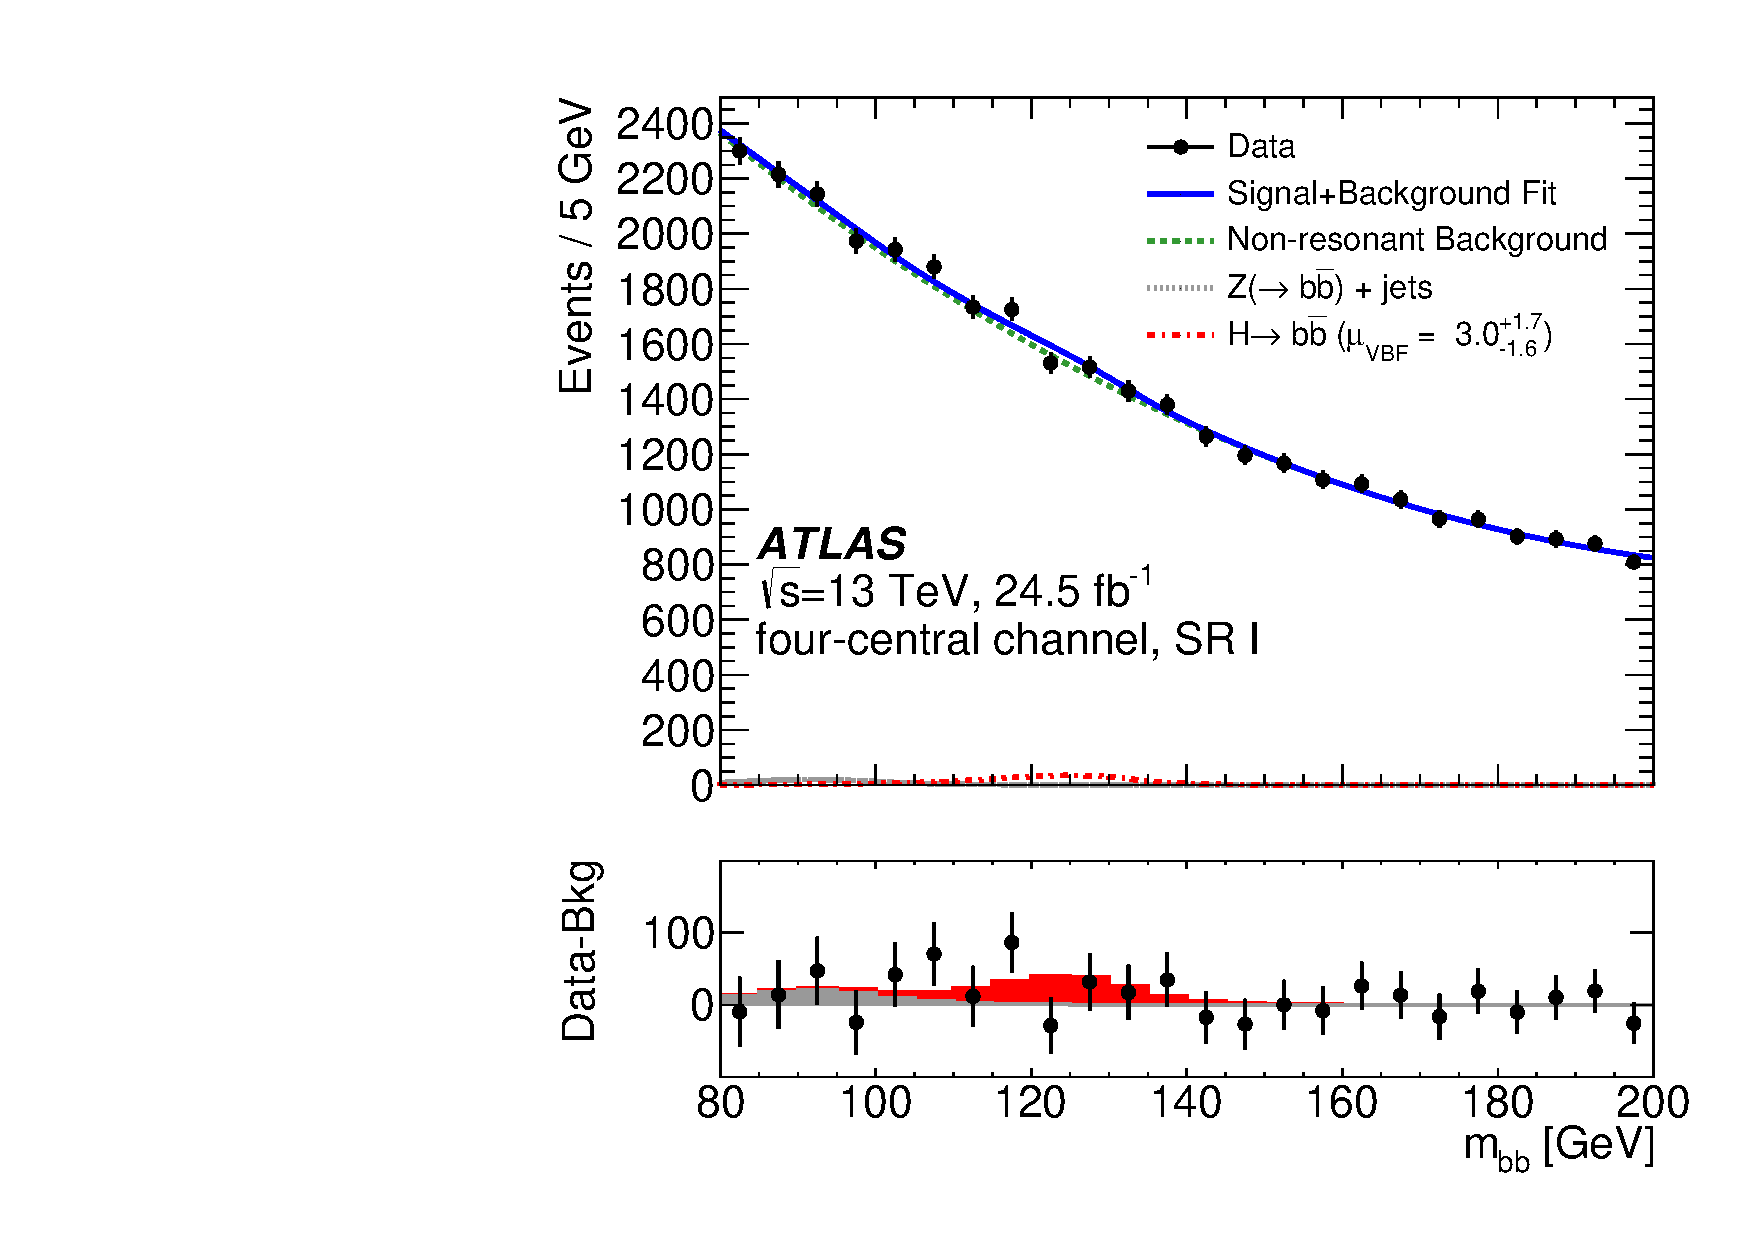
\includegraphics[width=0.48\textwidth]{figures/VBF/comb_vbfonly_testVBF_ICHEP_4cen_SRI_vbfincl.pdf}
 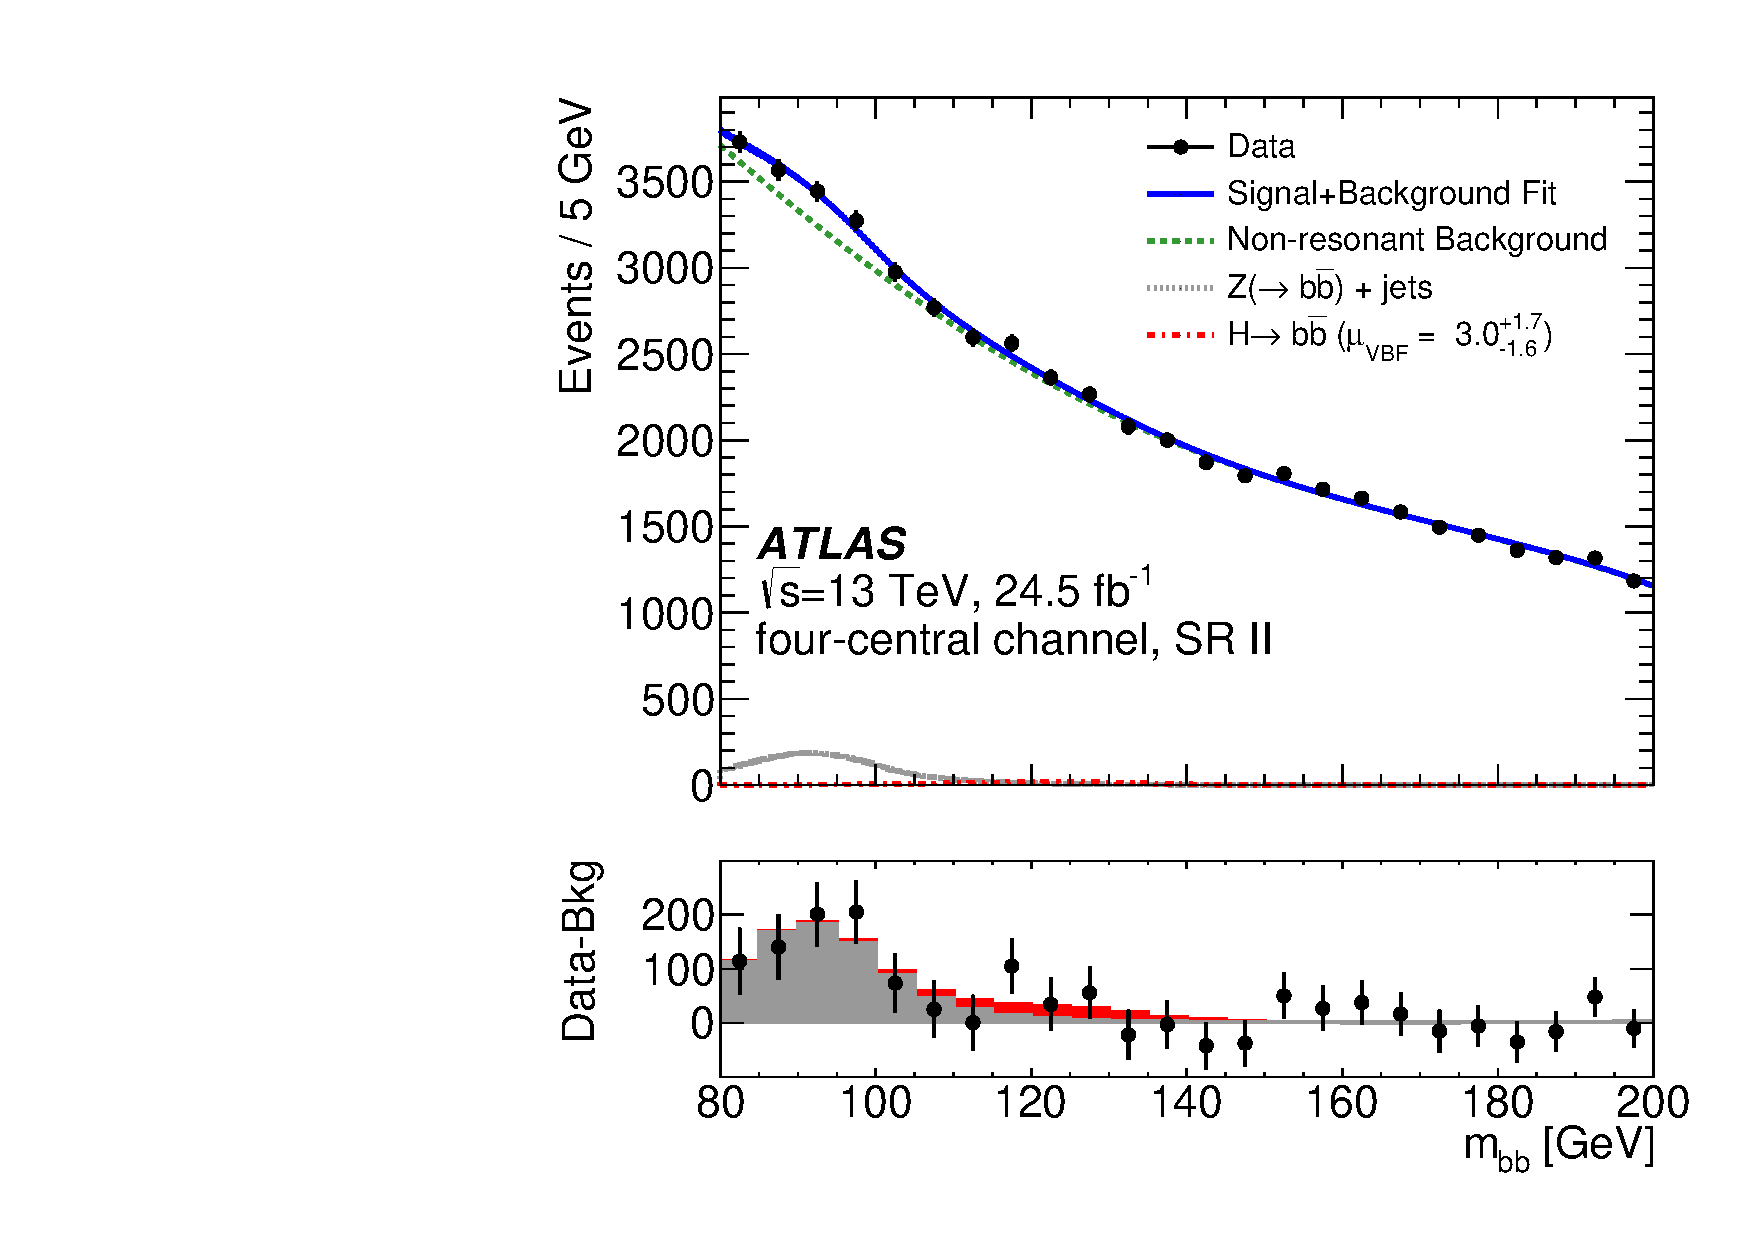
\includegraphics[width=0.48\textwidth]{figures/VBF/comb_vbfonly_testVBF_ICHEP_4cen_SRII_vbfincl.pdf}\\
 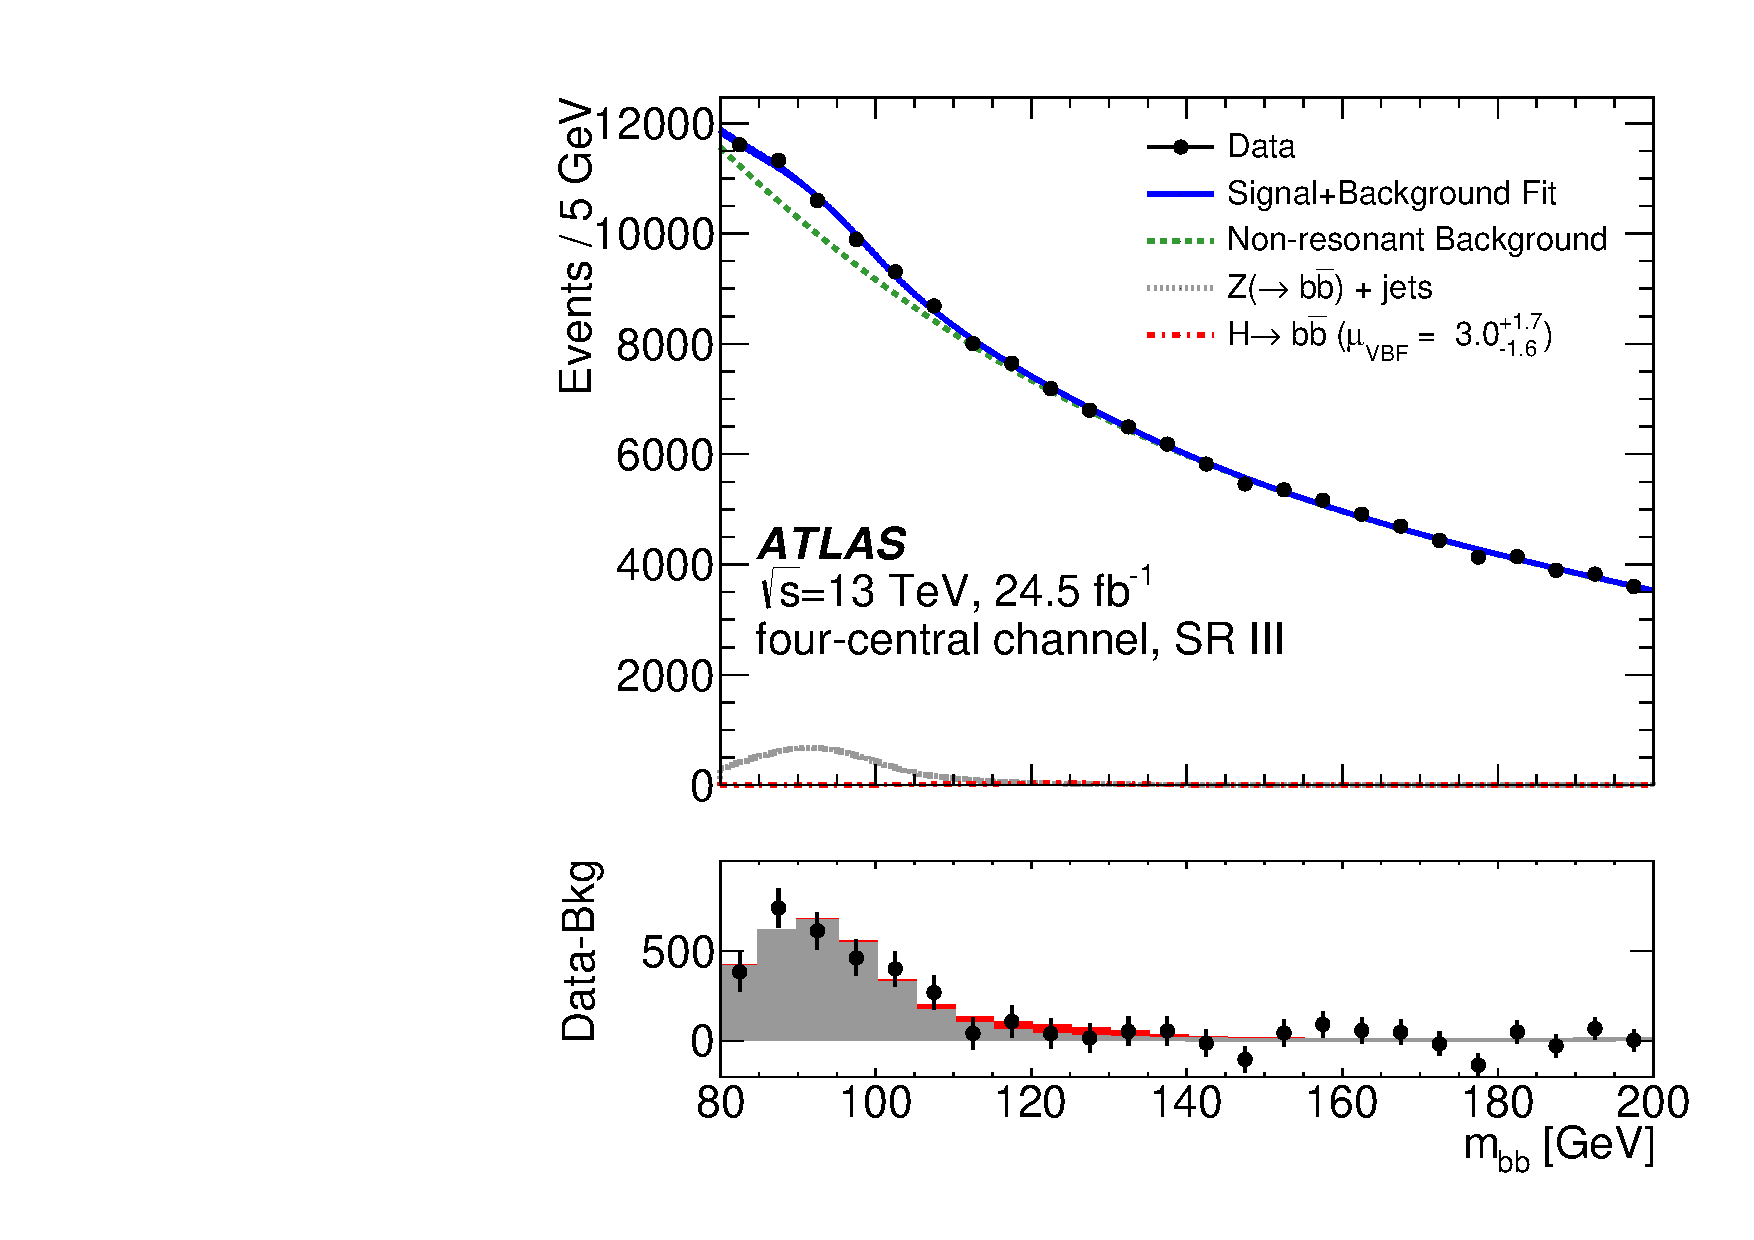
\includegraphics[width=0.48\textwidth]{figures/VBF/comb_vbfonly_testVBF_ICHEP_4cen_SRIII_vbfincl.pdf}
 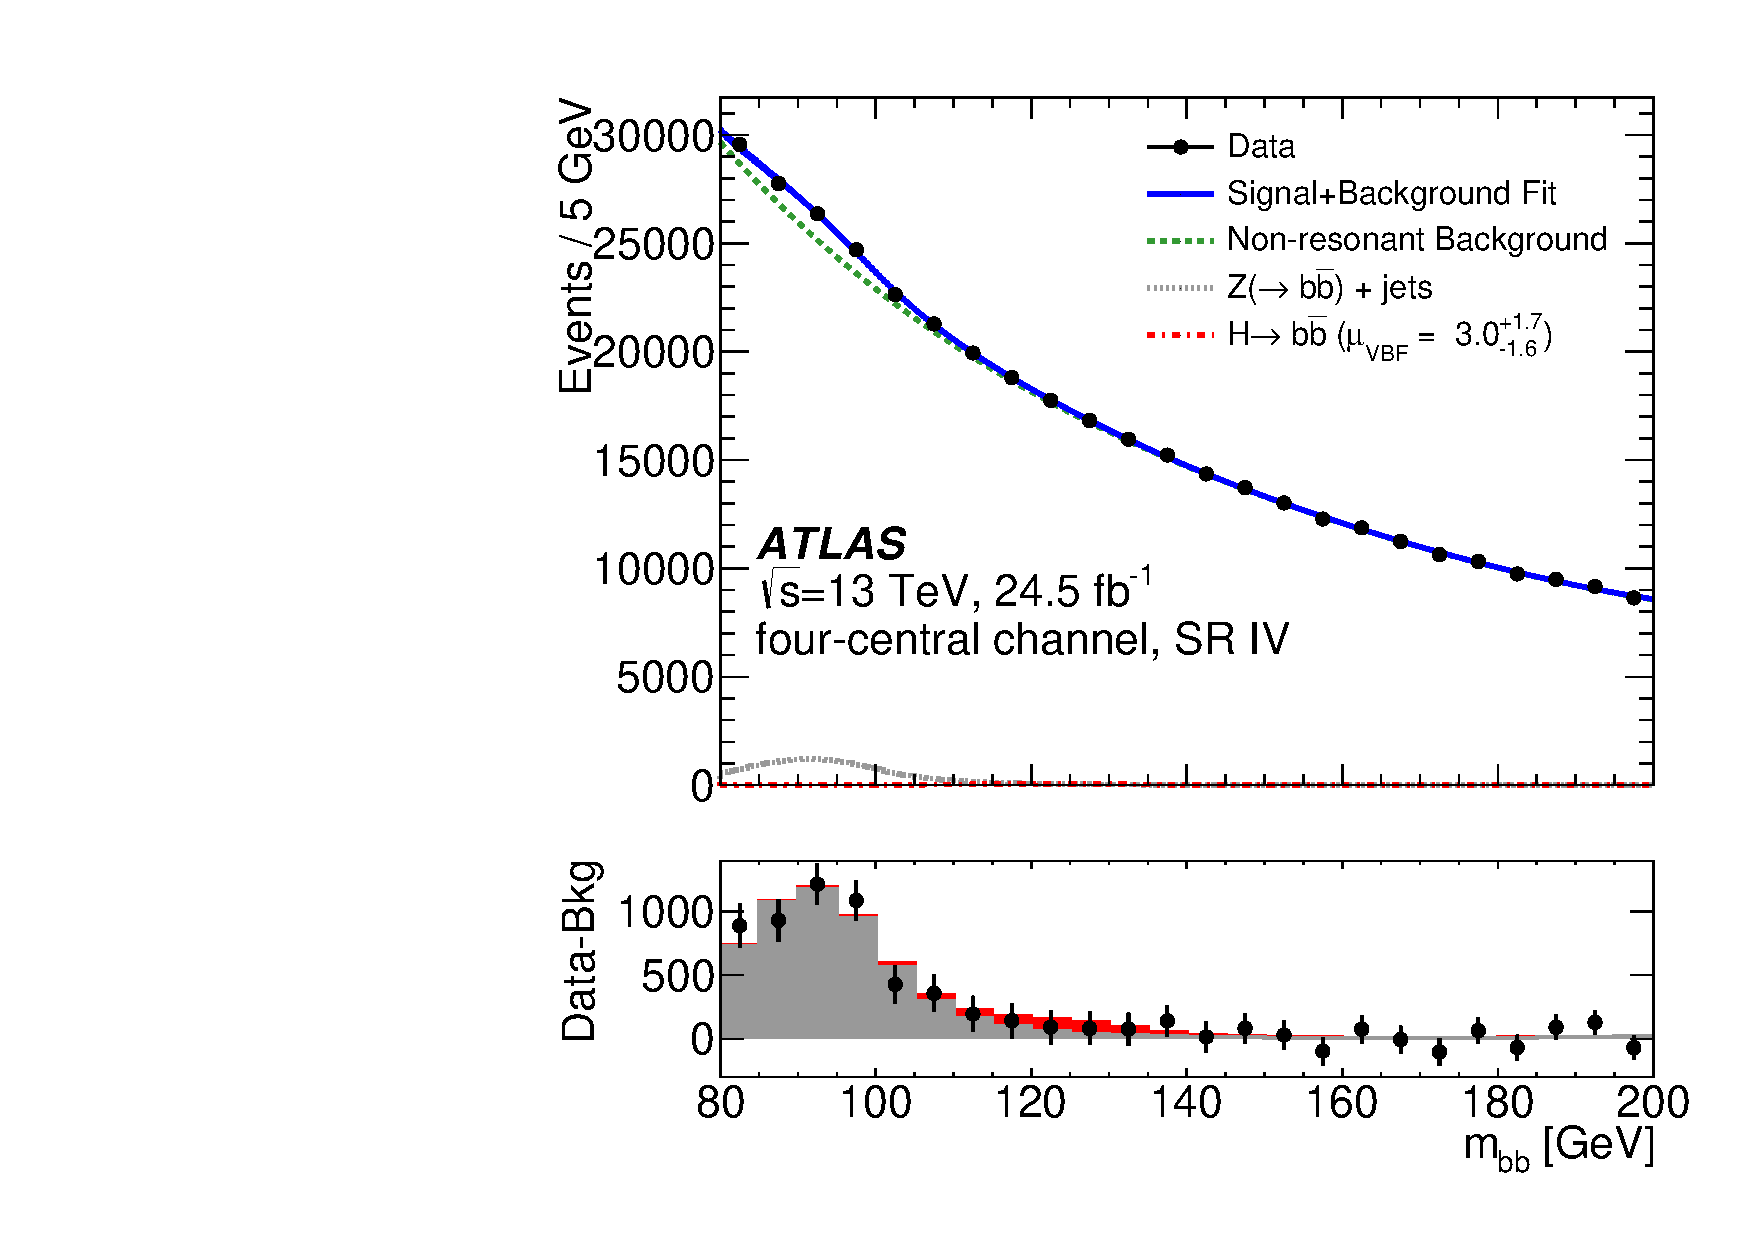
\includegraphics[width=0.48\textwidth]{figures/VBF/comb_vbfonly_testVBF_ICHEP_4cen_SRIV_vbfincl.pdf}\\

\caption{Data and fit model comparison for the combined fit of $\mu_{VBF}$ extraction in the \fourcentral channel}
  \label{fig:higgsfit_4cen}
\end{figure}



\begin{figure}[htbp]
\centering

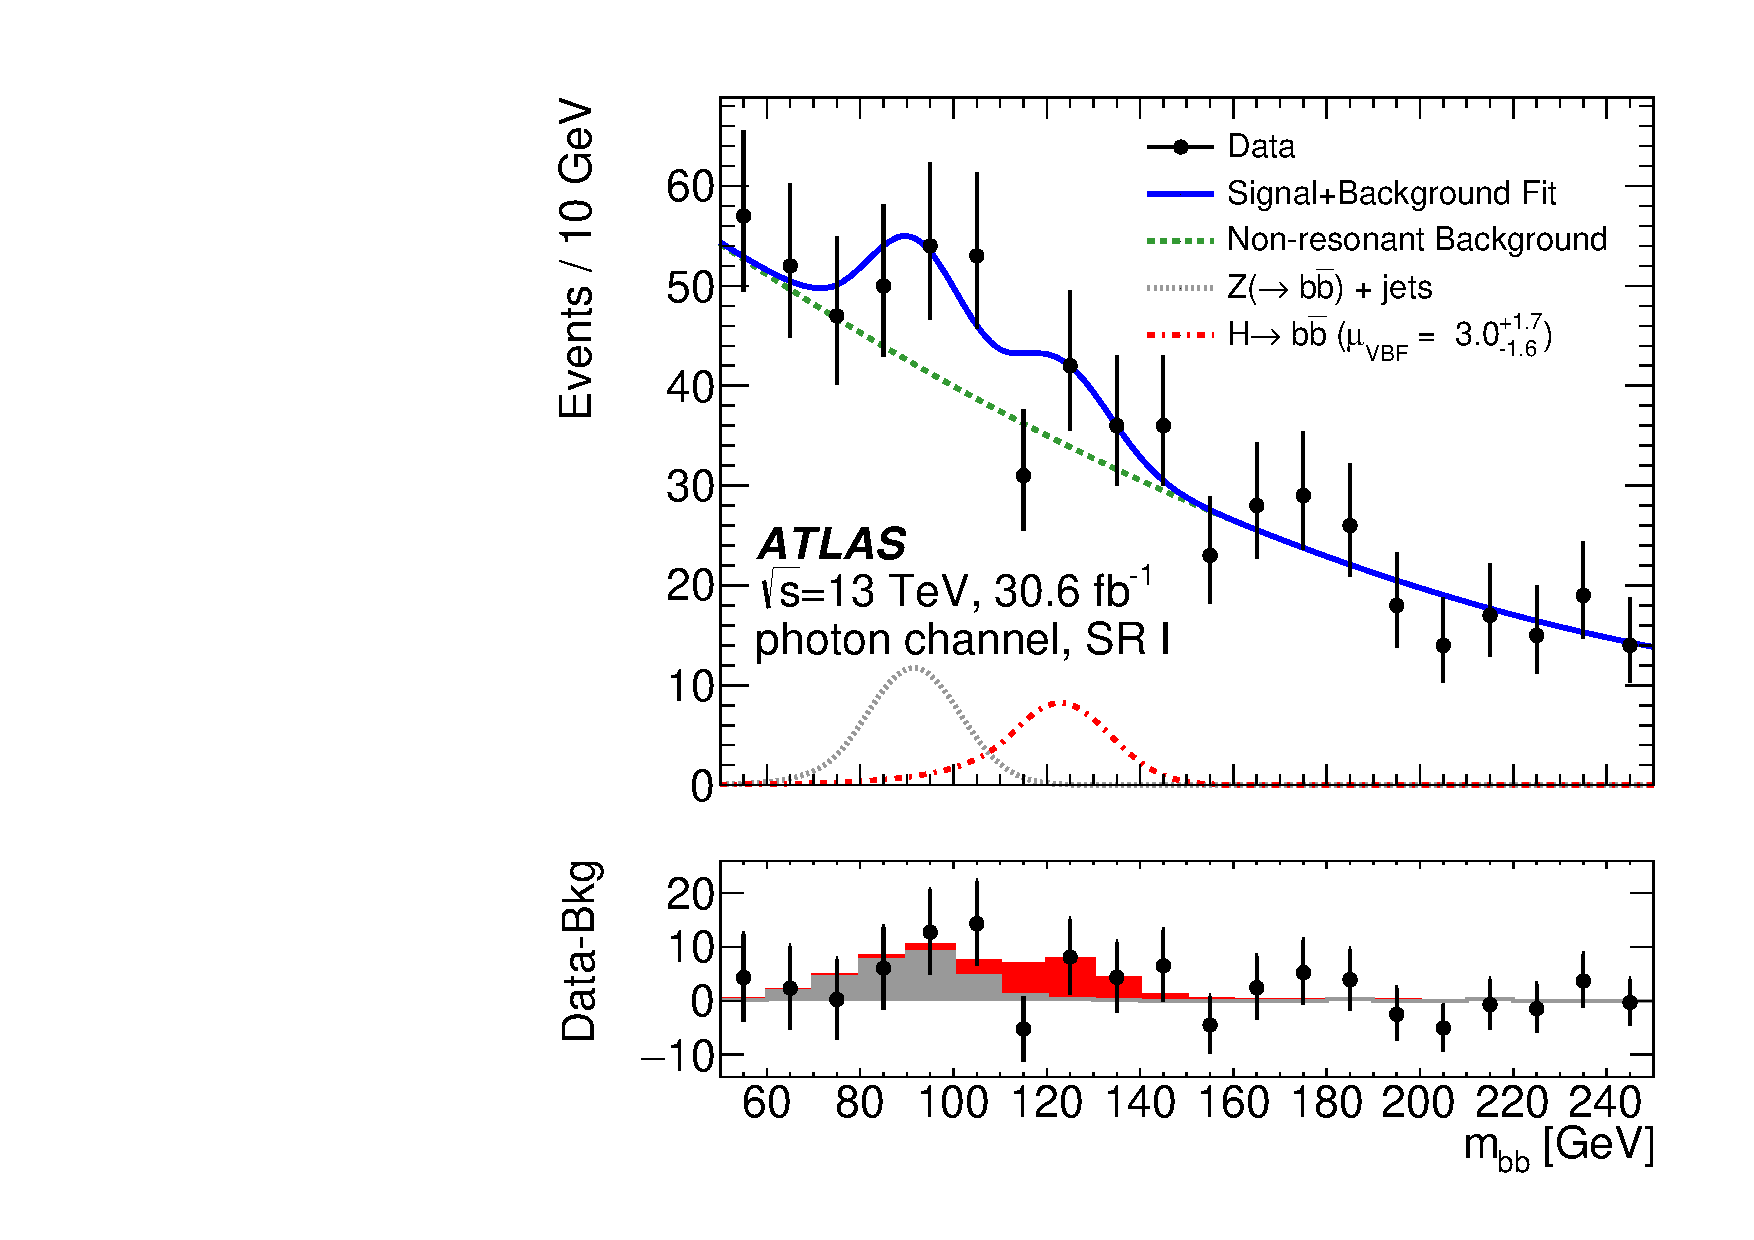
\includegraphics[width=0.48\textwidth]{figures/VBF/comb_vbfonly_testchannel1_vbfg.pdf}
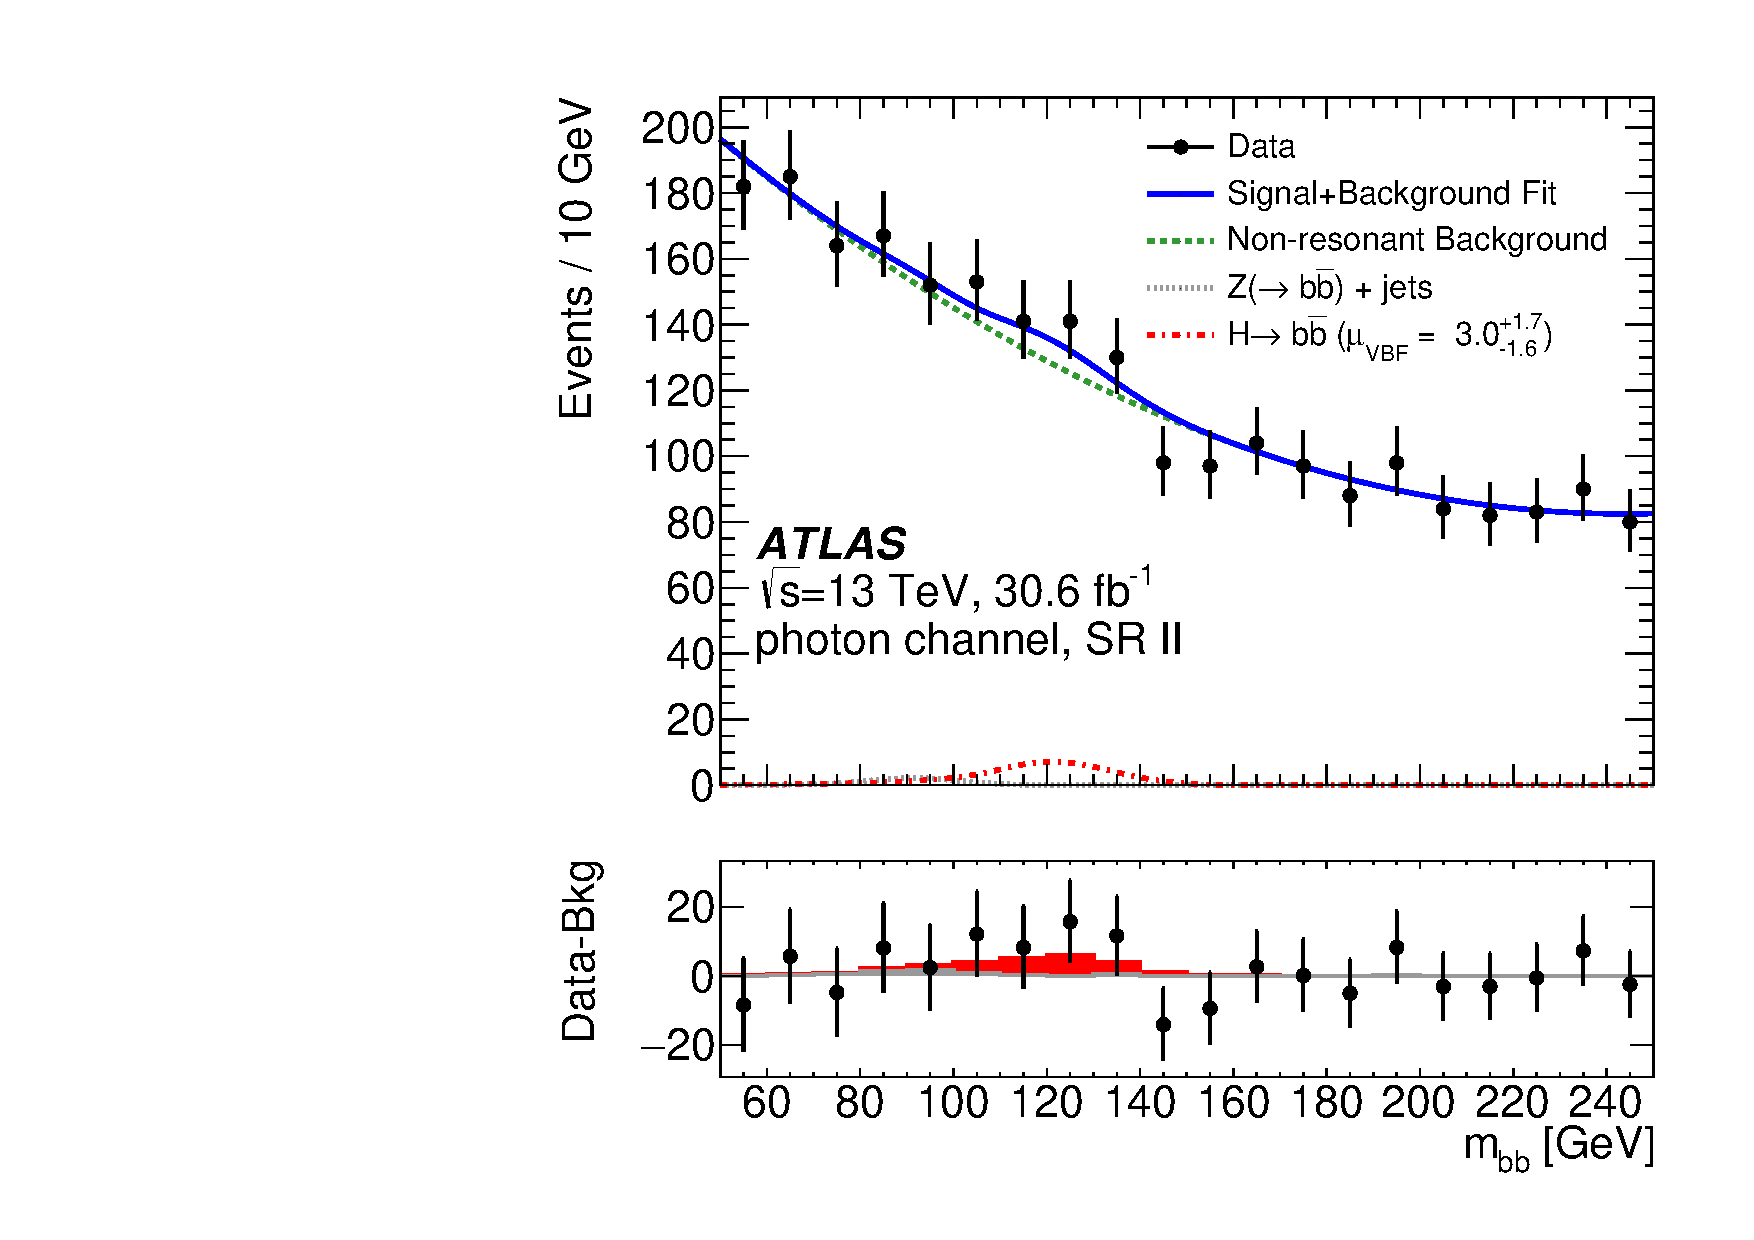
\includegraphics[width=0.48\textwidth]{figures/VBF/comb_vbfonly_testchannel2_vbfg.pdf}
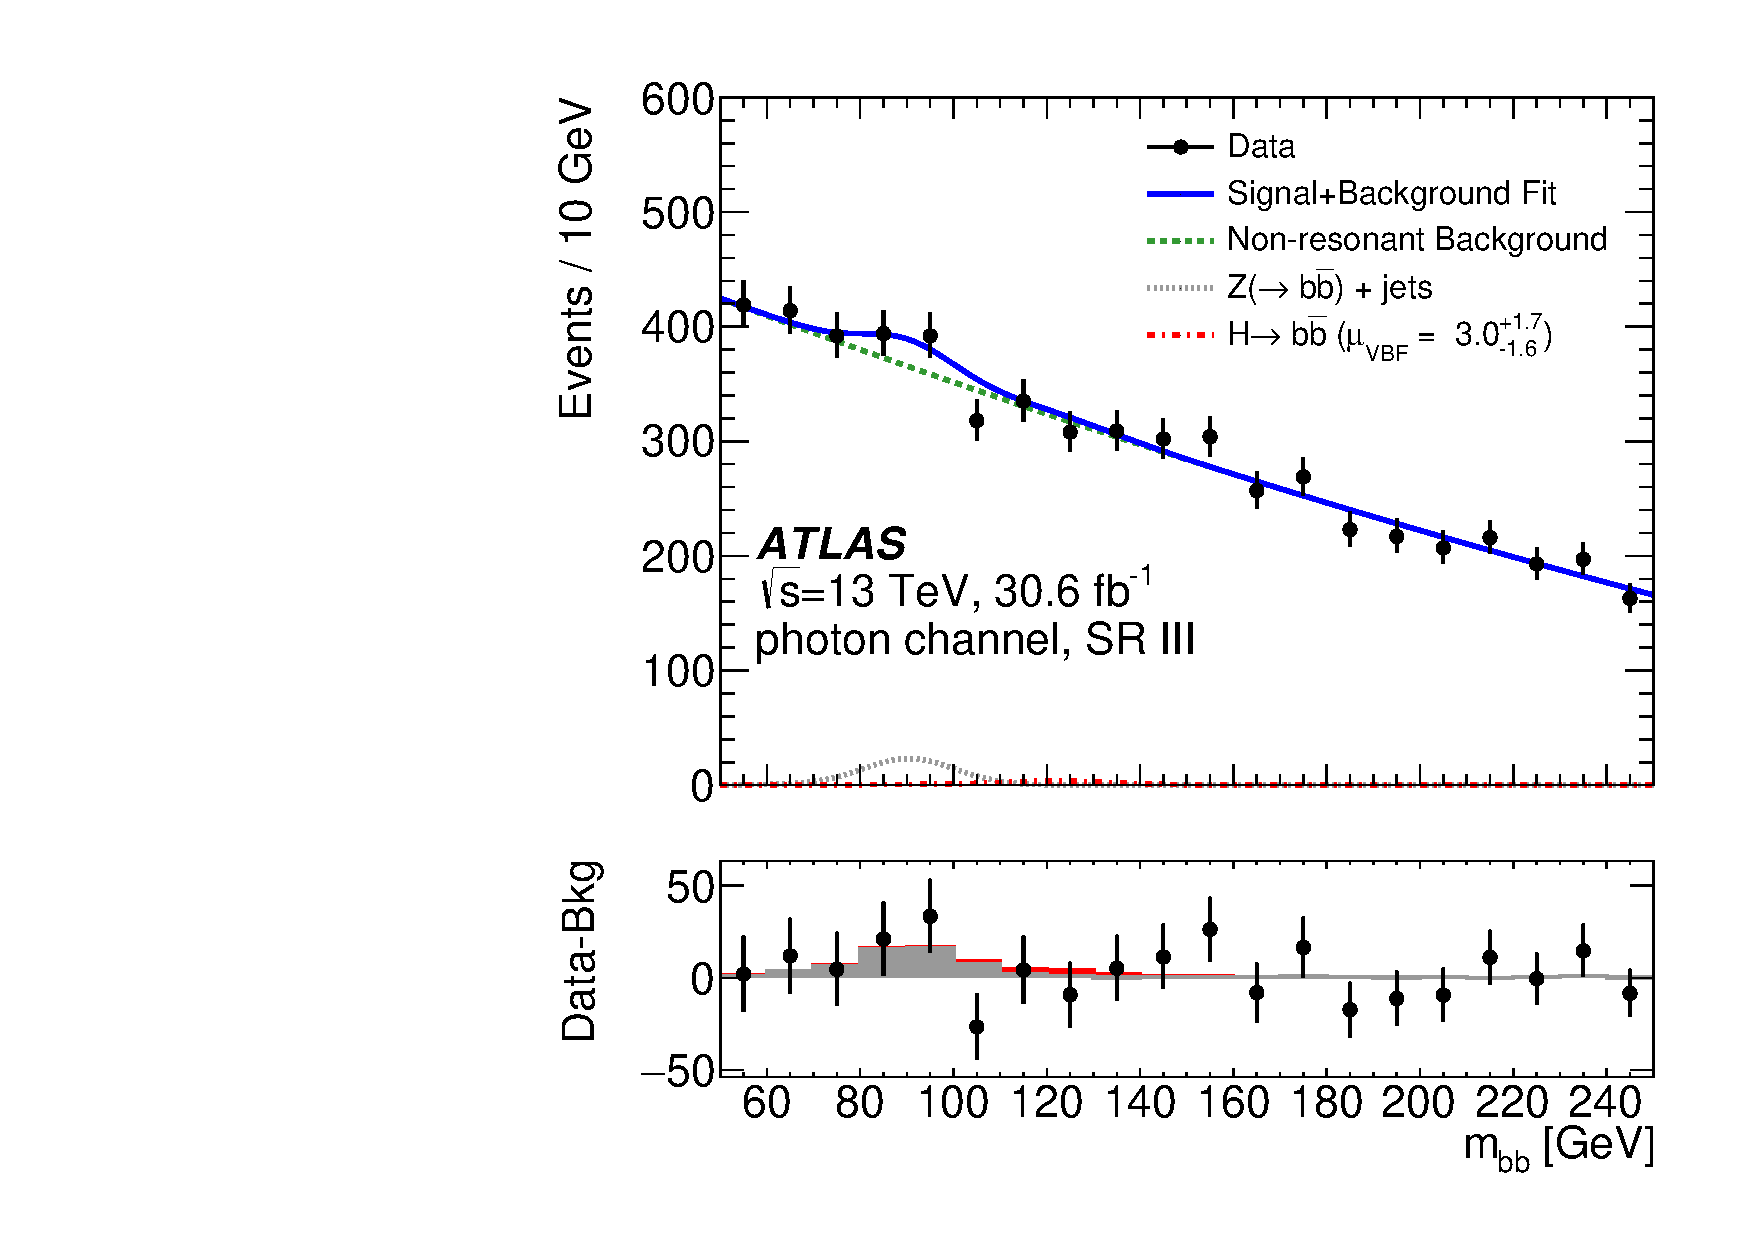
\includegraphics[width=0.48\textwidth]{figures/VBF/comb_vbfonly_testchannel3_vbfg.pdf}
\caption{Data and fit model comparison for the combined fit of $\mu_{VBF}$ extraction in the \textit{photon} channel}
\label{fig:mbb_postfit_photon}
\end{figure}


\begin{figure}[htbp]
  \centering
  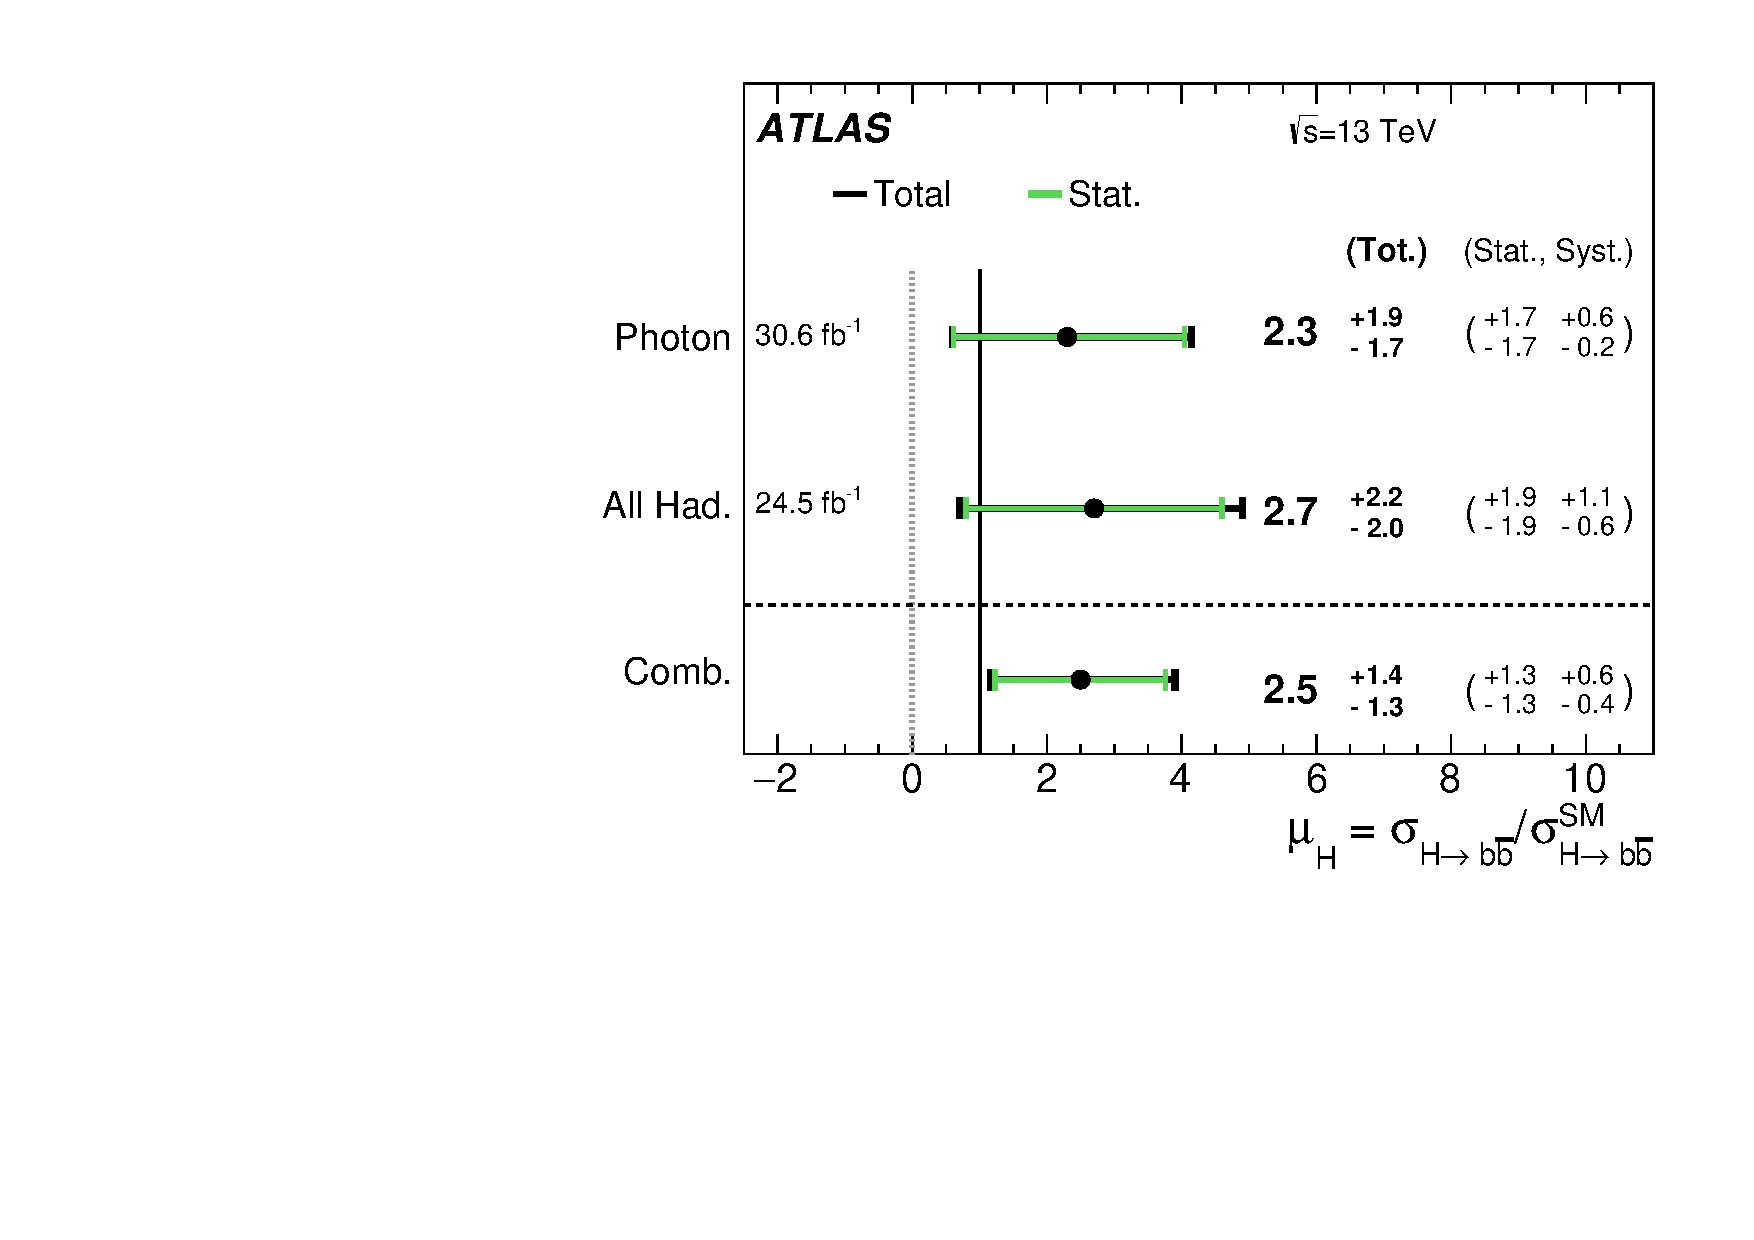
\includegraphics[width=0.49\textwidth]{figures/VBF/Plot_mu_summary_VBF.pdf}
  \includegraphics[width=0.49\textwidth]{figures/VBF/Plot_mu_summary_VBFonly.pdf}

\caption{Summary of the extraction of $\mu_{H}$(left) and $\mu_{VBF}$(right) for  \textit{all-hadronic}, \textit{photon} and combination fits.}
  \label{fig:vbf-summary}
\end{figure}



%\begin{figure}[htbp]
%  \centering
% \includegraphics[width=0.8\textwidth]{figures/VBF/VBFHbb_pulls_125.pdf}
% \caption{Nuisance parameter post-fit impact and pulls are plotted for the data fit. Only the constrained NPs are shown. The uncertainties follow the naming defined in Table. \ref{tab:systnames}.}
%  \label{fig:vbf-higgsfitpull}
%\end{figure}

Regarding the treatment of uncertainties, both the inclusive and photon analyses apply systematics trimming. The inclusive analyses ignore nuisance parameters with yield impact $<0.5\%$ while the photon analysis ignore systematics with yield impact $<1\%$. Some NPs, for instance the third effective NP of jet energy scale may pass the systematics trimming cut of one analysis but not the other and therefore only show up in the combination fit for one analysis. 

Same set of nuisance parameters of detector related uncertainties including jet energy scale/resolution, luminosity, pile-up reweighting and q/g tagging is used by both analyses and hence treated as correlated.  $b$-tagging related uncertainties are an exception because the operating points are different between the two analyses. The inclusive analysis uses 70\% and 85\% WPs for \twocentral and \fourcentral channels respectively and the VBF$+\gamma$ analysis uses the 77\% WP. We experimented correlating NPs of the $b$-tagging uncertainties with highest impact, e.g. alpha\_FT\_EFF\_Eigen\_B\_0 of different WPs, across the two analyses and observed negligible change in the final result. Therefore the $b$-tagging NPs are left to be un-correlated.

Common terms of theoretical uncertainties including QCD scale of VBF process, parton shower and variation of $ttH$ yield are also correlated as the underlying variations are derived with same approaches. Background systematics such as non-resonant background normalization/parameterization, Z normalization and spurious signals are specific to each analysis and are not correlated.

The combination fit pull for $\mu_H$ is shown in Fig.\ref{fig:vbf-higgsfitpull_combination}. The combination fit pull for $\mu_{VBF}$ is shown in Fig.\ref{fig:vbf-vbffitpull_combination}. None of the systematics nuisance parameters are pulled significantly from their central values. One event display for the SRI of the \twocentral channel, the most sensitive BDT region, is shown in Fig.\ref{fig:vbf-evtdisplay}.


%%% no longer needed as VBF inclusive breaks down the QCD scale for VBF and ggF separately:  The inclusive and VBF$+\gamma$ analyses have some overlaps in the treatment of the QCD scale uncertainty although do not use exactly the same procedure therefore, by default, it is treated as uncorrelated.  The VBF$+\gamma$ analysis generates samples at truth level with changes by factors of two in the QCD scale and then does a truth-level calculation of the impact on the acceptance and normalization.  This analysis uses weights generated according to the \textit{WG1 scheme} (see Section~\ref{sec:vbf-syst_model}). Since it is a large systematic uncertainty for both analyses, we also try to correlate this particular nuisance parameter. The combined fit correlating the QCD scale uncertainty yields $\mu_H = 2.40^{+1.37}_{-1.32}$, which has a negligible difference with respect to the uncorrelated treatment. Hence we eventually adopt the result treating QCD scale as un-correlated as it is a more conservative approach. 


\begin{figure}[htbp]
  \centering
 \includegraphics[width=0.8\textwidth]{figures/VBF/VBFHbb_Combined_pulls_125.pdf}
\caption{Data fit pulls for nuisance parameters with a post-fit impact $> 2$ \% for $\mu_H$ combining VBF inclusive and VBF$+\gamma$ analyses.}
  \label{fig:vbf-higgsfitpull_combination}
\end{figure}

\begin{figure}[htbp]
  \centering
 \includegraphics[width=0.8\textwidth]{figures/VBF/VBFHbb_Combined_vbfonly_pulls_125.pdf}
\caption{Data fit pulls for nuisance parameters with a post-fit impact $> 2$ \% for $\mu_{VBF}$ combining VBF inclusive and VBF$+\gamma$ analyses.}
  \label{fig:vbf-vbffitpull_combination}
\end{figure}


\begin{figure}[htbp]
  \centering
 \includegraphics[width=0.8\textwidth]{figures/VBF/EvtDisplay2cen}
\caption{Event display of a \twocentral candidate event in SR I of the with \Mbb = 147 GeV. The cones representing the jets are colored magenta for the forward jets and orange for the b-tagged jets. The transverse momenta of the leading forward jet and sub-leading forward jet are 130.5 GeV and 82.0 GeV respectively. The pseudorapidity of the leading forward jet and sub-leading forward jet are -2.0 and 3.6 respectively}
  \label{fig:vbf-evtdisplay}
\end{figure}



% All figures and tables should appear before the summary and conclusion.
% The package placeins provides the macro \FloatBarrier to achieve this.
% \FloatBarrier

%-------------------------------------------------------------------------------
\section{Conclusion}
\label{sec:conclusion}
%-------------------------------------------------------------------------------

We have performed a search for Higgs boson decays to $b$-quarks in a sample enriched in events produced by vector boson fusion. A fitted signal strength for $H\rightarrow bb$, $\mu_H$, of $2.7^{+2.2}_{-2.0}$ is observed, compared to an expectation of $1.0^{+1.9}_{-1.9}$. A fitted signal strength for VBF $H\rightarrow bb$, $\mu_{VBF}$, of $4.1^{+3.2}_{-2.9}$ is observed, compared to an expectation of $1.0^{+2.8}_{-2.8}$.  A combined fit with an analysis targeting $H\rightarrow b\bar{b}$ with the addition of a photon, yields $\mu_H = 2.5^{+1.4}_{-1.3}$ corresponding to an observed significance of $1.9\sigma$ ($0.8\sigma$ expected). A combined fit for $\mu_{VBF} = 3.0^{+1.7}_{-1.6}$ corresponds to an observed significance of $1.9\sigma$ ($0.7\sigma$ expected). 


%-------------------------------------------------------------------------------
\clearpage
\appendix
\part*{Appendix}
\addcontentsline{toc}{part}{Appendix}
%-------------------------------------------------------------------------------

%-------------------------------------------------------------------------------
\clearpage
\section{VBF Jets Kinematics}
\label{sec:app-kinematics}
We present the kinematics of the VBF jets in the signal and background events. The $\eta$, $p_{T}$ and number of jets distributions after the pre-selection cuts described in Section~\ref{sec:evtsel} are shown in Figures~\ref{fig:NJets}~to~\ref{fig:VBFeta}.  J1 refers to the higher $\pT$ VBF jet, J2 is the lower \pT of the pair. We also present the PU fraction of \twocentral channel as a function of the $\Delta|\eta|$ of two VBF jets in \ref{fig:PUdelta}.


\begin{figure}[htbp]
  \centering
 \includegraphics[width=0.48\textwidth]{figures/App-NJets_2cen.pdf}
 \includegraphics[width=0.48\textwidth]{figures/App-NJets_4cen.pdf}

\caption{Distributions of number of jets after pre-selection of \twocentral channel (left) and  \fourcentral channel (right)}
  \label{fig:NJets}
\end{figure}


\begin{figure}[htbp]
  \centering
 \includegraphics[width=0.48\textwidth]{figures/App-pTJ1_2cen.pdf}
 \includegraphics[width=0.48\textwidth]{figures/App-pTJ2_2cen.pdf}\\
 \includegraphics[width=0.48\textwidth]{figures/App-pTJ1_4cen.pdf}
 \includegraphics[width=0.48\textwidth]{figures/App-pTJ2_4cen.pdf}\\

\caption{$p_{T}$ distributions of VBF jets of \twocentral channel (top) and  \fourcentral channel (bottom)}
  \label{fig:VBFpT}
\end{figure}


\begin{figure}[htbp]
  \centering
 \includegraphics[width=0.48\textwidth]{figures/App-EtaJ1_2cen.pdf}
 \includegraphics[width=0.48\textwidth]{figures/App-EtaJ2_2cen.pdf}\\
 \includegraphics[width=0.48\textwidth]{figures/App-EtaJ1_4cen.pdf}
 \includegraphics[width=0.48\textwidth]{figures/App-EtaJ2_4cen.pdf}\\

\caption{$\eta$ distributions of VBF jets of \twocentral channel (top) and  \fourcentral channel (bottom)}
  \label{fig:VBFeta}
\end{figure}

\begin{figure}[htbp]
  \centering
 \includegraphics[width=0.48\textwidth]{figures/App-PUFrac-2cen.png}
\caption{PU fraction as a function of $\Delta|\eta|$ of VBF jets for \twocentral channel.}
  \label{fig:PUdelta}
\end{figure}


%-------------------------------------------------------------------------------
\clearpage
\section{BDT} 
\label{sec:app-bdt}
The BDT score and its correlation with \Mbb are checked for data and VBF signal Monte Carlo. We observe negligible linear correlation in Figures~\ref{fig:Mbb_BDT_VBF} and ~\ref{fig:Mbb_BDT_data}.  The correlation is largest in the signal for masses below 100~\GeV where lower BDT values are preferred. The low \Mbb{} correlation is expected because these are likely cases with FSR which lower \Mbb~and change the jet kinematics.  For the background the correlation is strongest for the \twocentral case, with a higher mass corrected with a more peaked BDT distribution. The Pearson correlation factors are 0.08 and -0.03 for data and VBF signal in \twocentral channel; -0.05 and -0.02 for data and VBF signal in \fourcentral channel.

To further study the BDT correlation with \Mbb{} we plot the profile \Mbb{} value versus BDT score in ~\ref{fig:BDT_Profile} for the \twocentral channel.  We observe that for high BDT values in the \twocentral channel the mean of the \Mbb value increases.  We also find that  the highest BDT values are correlated with very high $p_T$ events, as shown in the same figure.  Figure~\ref{fig:MBB_pTBB} shows that high \pTbb{} events do not populate the low \Mbb{} spectrum, which further explains the observation in the preceding paragraph. This could cause a turn-on, which is difficult to model with an analytical function.  Therefore we cut moderately on the BDT score for the most sensitive BDT region to reduce these turn on effects. 

The sensitivity of the variables we consider are shown in Tables \ref{tab:BDT-2cen-sensitivity} and \ref{tab:BDT-4cen-sensitivity}. We calculate the sensitivity of every variable by leaving out one variable at a time from the list we consider and train a new BDT. The most sensitive variables we find are the $q$/$g$ discriminants NTrk500 for the VBF jets. Since the HT variable has small impact on sensitivity and bad modeling in MC we choose not to include it in the final list of BDT input. 

A 3-fold cross validation of the BDT hyper-parameter choice is performed to limit the problem of overfitting. The entire signal and background sample is divided into three random subset with equal number of events. For each test, a BDT is trained with one subset and tested on the other two subsets. Table \ref{tab:BDT-2cen-kfold} presents the sensitivity of each validation test. The hyper-parameters used for building the nominal BDT generate BDTs of similar discrimination power in subsets of the entire sample. 

As the nominal analysis uses the BDT trained with half of the sideband data, a potential bias could arise if there is a significant difference in the numbers of events predicted in the sidebands of training and test sample. If such a difference exists, one could argue that since the mass window data is unseen in the BDT training procedure, the training set mass window data would behave the same way as the test set and hence create a deficit or excess compared to the hypothetical training procedure in which the mass window background data is used for BDT training. This potential bias is studied in three ways. First the numbers of events in sidebands of training and test samples are compared as shown in Fig.\ref{fig:bdt_evt_sidebands}. The differences in most of the regions are not statistically significant. Secondly, the data fit is separately performed for training and test set. The results as summarized in Fig. \ref{fig:separatefit} which shows the fit results are quite compatible and the difference is way smaller than the quoted uncertainties. Finally, to fully disentangle the statistical and systematic effects which are mixed in the data fits, Asimov test with reweighting is performed. The non-resonant background of Asimov dataset is built with sideband only fit. The sideband of the non-resonant background in Asimov dataset is then re-weighted by the ratios measured from the data sideband comparisons. Higgs signal and Z background are injected at strength of $\mu=1$. The measured Higgs signal strength of re-weighted Asimov is $\mu=1.18$ which gives an upper bound of the potential bias for the inclusive analysis of $\Delta \mu = 0.18$. When combined with the photon analysis the bias would be around $\Delta \mu = 0.1$ smaller than the leading the systematic uncertainties quoted in the paper. Hence this bias is not significant and ignored. 


\begin{figure}[htbp]
  \centering
 \includegraphics[width=0.48\textwidth]{figures/Mbb_BDT_VBF_2cen.pdf}
 \includegraphics[width=0.48\textwidth]{figures/Mbb_BDT_RowNorm_VBF_2cen.pdf}\\
 \includegraphics[width=0.48\textwidth]{figures/Mbb_BDT_VBF_4cen.pdf}
 \includegraphics[width=0.48\textwidth]{figures/Mbb_BDT_RowNorm_VBF_4cen.pdf}\\

\caption{VBF signal distributions of $M_{b\bar b}$ Vs. BDT Score for 2 central (top) and 4 central (bottom). The nominal distribution is on left and the distribution with integral of each row normalized to 1 is on right.}
  \label{fig:Mbb_BDT_VBF}
\end{figure}


\begin{figure}[htbp]
  \centering
 \includegraphics[width=0.48\textwidth]{figures/Mbb_BDT_data_2cen.pdf}
 \includegraphics[width=0.48\textwidth]{figures/Mbb_BDT_RowNorm_data_2cen.pdf}\\
 \includegraphics[width=0.48\textwidth]{figures/Mbb_BDT_data_4cen.pdf}
 \includegraphics[width=0.48\textwidth]{figures/Mbb_BDT_RowNorm_data_4cen.pdf}\\

\caption{Data distributions of $M_{b\bar b}$ Vs. BDT Score for 2 central (top) and 4 central (bottom). The nominal distribution is on left and the distribution with integral of each row normalized to 1 is on right.}
  \label{fig:Mbb_BDT_data}
\end{figure}


\begin{figure}[htbp]
  \centering
 \includegraphics[width=0.48\textwidth]{figures/Profile_BDT_mBB.pdf}
 \includegraphics[width=0.48\textwidth]{figures/Profile_BDT_pTBB.pdf}\\

\caption{Profile plots for \Mbb(left) and \pTbb(right) vs. the BDT discriminant for \twocentral channel}
  \label{fig:BDT_Profile}
\end{figure}


\begin{figure}[htbp]
  \centering
 \includegraphics[width=0.6\textwidth]{figures/MBB_pTBB.pdf}
\caption{\twocentral channel \Mbb vs. \pTbb}
  \label{fig:MBB_pTBB}
\end{figure}


\begin{table}[]
\centering
\caption{The sensitivity ($S/\sqrt(B)$) of \twocentral BDT leaving out one input variable at a time. The sensitivity is estimated with cuts retaining top 20\%, 20\%-40\% and top 40\% events of VBF signal events.}
\label{tab:BDT-2cen-sensitivity}
\begin{tabular}{l|l|l|l|}
\cline{2-4}
 & $S/\sqrt(B)$      & Top 20\% & 20\%-40\% \\ \cline{2-4} 
 & $p_T$ balance     & 0.75     & 0.46      \\ \cline{2-4} 
 & $p_{JJ}$          & 0.77     & 0.48      \\ \cline{2-4} 
 & min$\Delta R$(J1) & 0.79     & 0.44      \\ \cline{2-4} 
 & min$\Delta R$(J2) & 0.77     & 0.46      \\ \cline{2-4} 
 & Max($\eta$)       & 0.82     & 0.49      \\ \cline{2-4} 
 & $m_{JJ}$          & 0.77     & 0.47      \\ \cline{2-4} 
 & $\eta^*$          & 0.80     & 0.49      \\ \cline{2-4} 
 & $\Delta m_{JJ}$   & 0.82     & 0.45      \\ \cline{2-4} 
 & $\cos{\theta}$    & 0.79     & 0.50      \\ \cline{2-4} 
 & NTrk500(J2)       & 0.81     & 0.48      \\ \cline{2-4} 
 & Full              & 0.83     & 0.49      \\ \cline{2-4} 
\end{tabular}
\end{table}


\begin{table}[]
\centering
\caption{The sensitivity ($S/\sqrt(B)$) of \fourcentral BDT leaving out one input variable at a time (esimated using Post-ICHEP data). The sensitivity is estimated with cuts retaining top 20\%, 20\%-40\% and top 40\% events of VBF signal events.}
\label{tab:BDT-4cen-sensitivity}
\begin{tabular}{l|l|l|l|}
\cline{2-4}
 & $S/\sqrt(B)$      & Top 20\% & 20\%-40\% \\ \cline{2-4} 
 & $p_T$ balance     & 0.54     & 0.41      \\ \cline{2-4} 
 & $p_{JJ}$          & 0.53     & 0.40      \\ \cline{2-4} 
 & min$\Delta R$(J1) & 0.55     & 0.4       \\ \cline{2-4} 
 & min$\Delta R$(J2) & 0.56     & 0.43      \\ \cline{2-4} 
 & Max($\eta$)       & 0.59     & 0.42      \\ \cline{2-4} 
 & $m_{JJ}$          & 0.58     & 0.41      \\ \cline{2-4} 
 & $\eta^*$          & 0.65     & 0.39      \\ \cline{2-4} 
 & $\Delta m_{JJ}$   & 0.55     & 0.3       \\ \cline{2-4} 
 & $\cos{\theta}$    & 0.62     & 0.42      \\ \cline{2-4} 
 & NTrk500(J1)       & 0.65     & 0.40      \\ \cline{2-4} 
 & NTrk500(J2)       & 0.53     & 0.42      \\ \cline{2-4} 
 & HT                & 0.57     & 0.31      \\ \cline{2-4} 
 & Full              & 0.69     & 0.39      \\ \cline{2-4} 
\end{tabular}
\end{table}


\begin{table}[]
\centering
\caption{The sensitivity ($S/\sqrt(B)$) of \twocentral BDT 3-fold test}
\label{tab:BDT-2cen-kfold}
\begin{tabular}{l|l|l|l|l|}
\cline{2-5}
 & $S/\sqrt(B)$ & Test 1 & Test 2 & Test 3 \\ \cline{2-5} 
 & Top 30\%     & 0.80   & 0.80   & 0.82   \\ \cline{2-5} 
 & 30\%-40\%    & 0.31   & 0.31   & 0.30   \\ \cline{2-5} 
\end{tabular}
\end{table}


\begin{table}[]
\centering
\caption{The sensitivity ($S/\sqrt(B)$) of \fourcentral BDT 3-fold test}
\label{tab:BDT-4cen-kfold}
\begin{tabular}{l|l|l|l|l|}
\cline{2-5}
 & $S/\sqrt(B)$ & Test 1 & Test 2 & Test 3 \\ \cline{2-5} 
 & Top 20\%     & 0.55   & 0.54   & 0.54   \\ \cline{2-5} 
 & 20\%-40\%    & 0.39   & 0.39   & 0.37   \\ \cline{2-5} 
\end{tabular}
\end{table}


\begin{figure}[htbp]
  \centering
 \includegraphics[width=0.45\textwidth]{figures_final/Canv_Giacinto_Check_ratio_2cen.png}
 \includegraphics[width=0.45\textwidth]{figures_final/Canv_Giacinto_Check_ratio_4cen.png}
\caption{Number of events in sidebands of training and test sample. The numbers of events predicted by BDT in training and test data samples are mostly statistically compatible. The most prominent difference is in SRI of \fourcentral region and is only $2\%$.}
  \label{fig:bdt_evt_sidebands}
\end{figure}

\begin{figure}[htbp]
  \centering
 \includegraphics[width=0.6\textwidth]{figures_final/Plot_mu_summary_Giacinto.pdf}
\caption{Data training and test sample fit summary. The fitted Higgs strengths obtained from full, training and test datasets are compatible within the uncertainties.}
  \label{fig:separatefit}
\end{figure}


%-------------------------------------------------------------------------------
\clearpage
\section{b-jet energy correction}
\label{sec:app-masscorrection}
We apply energy corrections to b-jets to improve the mass resolution of the final discriminant $M_{b\bar b}$. Two steps of corrections are applied, which are muon in jet correction and PtReco correction. The muon in jet correction adds back the four-vector of soft muon inside the b-jet to b-jet four-vector. After muon in jet correction, the PtReco correction corrects the energy of the b-jet so that the Reco level $M_{b \bar b}$ has the same peak value as the particle level jets in $VH \rightarrow llb \bar b$ process. The nominal and corrected $M_{b \bar b}$ distributions are shown in Figure~\ref{fig:MbbCorrection}. After the correction, 88\% of the VBF signal events end up in the mass window [100, 140] GeV which we extract signal, while 7\% leaks into the lower side-band and 5\% leadks into the upper side-band. Same distributions for $Z\rightarrow b \bar b$ are shown in Figure ~\ref{fig:MbbCorrection_Z}.

\begin{figure}[htbp]
  \centering
 \includegraphics[width=0.5\textwidth]{figures/Mbb_Correction.pdf}

\caption{$M_{b \bar b}$ distributions of nominal and corrected b-jet energy after pre-selection of VBF events. The mean and RMS of the distribution are improved after each correction.  }
  \label{fig:MbbCorrection}
\end{figure}


\begin{figure}[htbp]
  \centering
 \includegraphics[width=0.5\textwidth]{figures/Mbb_Correction_Z.pdf}

\caption{$M_{b \bar b}$ distributions of nominal and corrected b-jet energy after pre-selection of $Z\rightarrow b \bar b$ events.}
  \label{fig:MbbCorrection_Z}
\end{figure}


%-------------------------------------------------------------------------------
%\clearpage
\section{$Z\rightarrow b \bar b$ Injection Test}
\label{sec:app-zinjection}
%The effect of floaing the normalization of the $Z\rightarrow b \bar b$ in the combined fit of \twocentral and \fourcentral channels is studied. The best fitted signal strength is $\hat \mu = 1.02 \pm 0.76$. The prediction of $Z$ events yield is found to be $alpha_z=3.89 \pm 0.93$ times the Standard Model prediction. The uncertainty is from the profile likelihood including the impact from all nuisance parameters. The fits are shown in Figures~\ref{fig:Fit_combined_znorm}. 

%Since the NLO k-factors for $Z$ yields vary with $Z$ \pT~and $Z$ decay product \pT, we also tried to allow the normalization of the $Z $component float freely in each BDT regions. The nuisance parameters of $Z$ normalization when each component is allowed to float are listed in Table. ~\ref{tab:z_float_all}. In this case, the best fitted signal strength is $\hat \mu = 2.06 \pm 0.97$. The small Z statistics in signal region make the Z component hard to constrain and leave the $\hat \mu$ biased and uncertainty inflated. The fits are shown in Figures~\ref{fig:Fit_combined_znorm_floatall}. 

{\it N.B. These studies were done with an earlier version of the BDT but the general results are expected to be the same.}

To estimate the impact on $\hat \mu$ of the Higgs signal caused by imprecise modeling of the $Z$ yield in different BDT regions, a $Z$ injection test using \twocentral channel is performed. Asimov datasets were built with a background function obtained from a background only fit.  In addition, the $Z$ signal is injected at a strength of $\mu_z= 0.5, 1.0, 2.0, 5.0, 1.0$ while fixing the Higgs signal to be that of the SM. Different strategies were tested including assigning one NP with Gaussian prior the overall $Z$ normalization (Figure~\ref{fig:zinjection_Con}), floating the overall $Z$ normalization (Figure~\ref{fig:zinjection_Float}) and constraining the $Z$ components with individual NPs with Gaussian priors in each BDT regions (Figure~\ref{fig:zinjection_ConAll}). The scenario of co-varying the $Z$ signal strengths and varying independently the $Z$ strengths across BDT regions are tested. In all fit models, we find that the bias of $\hat \mu$ of Higgs is around 5\% if the variations of $Z$ signal strength are within a factor of 2 of SM prediction, while the bias increases to 10\% if we expect a factor of 5 variation of SM prediction. The fit model starts to give large bias (20\%) if the $Z$ strength is mis-modeled by a factor of 10. 

Since the di-jet mass turn-on happens right around 80 GeV, requiring us to choose the fit starting point close to the $Z$ peak, the analytical function used to describe the non-resonant background lacks a constraint at the low end and becomes degenerate with the $Z$ peak. The major contribution of $Z$ component comes from QCD production, which is classified in a similar way as the QCD background by the BDT.  Most of the $Z$ events passing the pre-selection end up in the CR, where the sensitivity is low.  For these reasons, the analysis is insensitive to the $Z$ component, and yields a biased $Z$ strength and with a larger uncertainty compared to Higgs signal as shown in Figure~\ref{fig:zmu}. The uncertainty of $Z$ strength if $\alpha_Z$ is left to float is between 4.4 to 4.8 for injected $Z$ strength between 0.5 to 10 times the SM prediction. 


%\begin{figure}[htbp]
%  \centering
% \includegraphics[width=0.48\textwidth]{figures/FitCombined/zfloat_testVBF_ICHEP_2cen_SRI.pdf}
% \includegraphics[width=0.48\textwidth]{figures/FitCombined/zfloat_testVBF_ICHEP_2cen_SRII.pdf}\\
% \includegraphics[width=0.48\textwidth]{figures/FitCombined/zfloat_testVBF_ICHEP_4cen_SRI.pdf}
% \includegraphics[width=0.48\textwidth]{figures/FitCombined/zfloat_testVBF_ICHEP_4cen_SRII.pdf}\\
%
%\caption{Pseudo data fit for both channels while the $Z\rightarrow b \bar b$ normalization is left to float. Fits of SR I (left) and SR II (right) for 2 central (top) and 4 central (bottom) are shown.}
%  \label{fig:Fit_combined_znorm}
%\end{figure}
%
%
%\begin{table}[]
%\centering
%  \caption{Z normalization nuisance parameters.  $2cen$ refers to the \twocentral regions, $4cen$ refers to the \fourcentral regions.}
%\label{tab:z_float_all}
%\begin{tabular}{|l|l|}
%\hline
%
%$\alpha_{2cen}(CR)$         & $3.76\pm 4.89$   \\ \hline
%$\alpha_{2cen}(SRI)$        & $52.47\pm 36.78$   \\ \hline
%$\alpha_{2cen}(SRII)$       & $14.63\pm 12.47$   \\ \hline
%$\alpha_{4cen}(CR)$         & $3.63\pm 1.46$   \\ \hline
%$\alpha_{4cen}(SRI)$        & $16.69\pm 50.76$   \\ \hline
%$\alpha_{4cen}(SRII)$       & $5.53\pm 2.95$   \\ \hline
%
%
%\end{tabular}
%\end{table}
%
%
%\begin{figure}[htbp]
%  \centering
% \includegraphics[width=0.48\textwidth]{figures/FitCombined/zfloatall_testVBF_ICHEP_2cen_SRI.pdf}
% \includegraphics[width=0.48\textwidth]{figures/FitCombined/zfloatall_testVBF_ICHEP_2cen_SRII.pdf}\\
% \includegraphics[width=0.48\textwidth]{figures/FitCombined/zfloatall_testVBF_ICHEP_4cen_SRI.pdf}
% \includegraphics[width=0.48\textwidth]{figures/FitCombined/zfloatall_testVBF_ICHEP_4cen_SRII.pdf}\\
%
%\caption{Pseudo data fit for both channels while the $Z\rightarrow b \bar b$ normalizations in each BDT region are left to float. Fits of SR I (left) and SR II (right) for 2 central (top) and 4 central (bottom) are shown.}
%  \label{fig:Fit_combined_znorm_floatall}
%\end{figure}


\begin{figure}[htbp]
  \centering
 \includegraphics[width=0.48\textwidth]{figures/zstudy/zcon_mu_uniform.pdf}
 \includegraphics[width=0.48\textwidth]{figures/zstudy/zcon_mu_SRI.pdf}\\
 \includegraphics[width=0.48\textwidth]{figures/zstudy/zcon_mu_SRII.pdf}
 \includegraphics[width=0.48\textwidth]{figures/zstudy/zcon_mu_CR.pdf}\\

\caption{Asimov data fit of Z-injection test applying signle NP with Gaussian prior to the $Z$ normalization in \twocentral channel.}
  \label{fig:zinjection_Con}
\end{figure}


\begin{figure}[htbp]
  \centering
 \includegraphics[width=0.48\textwidth]{figures/zstudy/zfloat_mu_uniform.pdf}
 \includegraphics[width=0.48\textwidth]{figures/zstudy/zfloat_mu_SRI.pdf}\\
 \includegraphics[width=0.48\textwidth]{figures/zstudy/zfloat_mu_SRII.pdf}
 \includegraphics[width=0.48\textwidth]{figures/zstudy/zfloat_mu_CR.pdf}\\

\caption{Asimov data fit of Z-injection test applying floating the overall $Z$ normalization in \twocentral channel.}
  \label{fig:zinjection_Float}
\end{figure}


\begin{figure}[htbp]
  \centering
 \includegraphics[width=0.48\textwidth]{figures/zstudy/zconall_mu_uniform.pdf}
 \includegraphics[width=0.48\textwidth]{figures/zstudy/zconall_mu_SRI.pdf}\\
 \includegraphics[width=0.48\textwidth]{figures/zstudy/zconall_mu_SRII.pdf}
 \includegraphics[width=0.48\textwidth]{figures/zstudy/zconall_mu_CR.pdf}\\

\caption{Asimov data fit of Z-injection test applying separate NPs with Gaussian prior to $Z$ normalization in each BDT regions in \twocentral channel.}
  \label{fig:zinjection_ConAll}
\end{figure}


\begin{figure}[htbp]
  \centering
 \includegraphics[width=0.48\textwidth]{figures/zstudy/zcon_alphaZ.pdf}
 \includegraphics[width=0.48\textwidth]{figures/zstudy/zfloat_alphaZ.pdf}\\

\caption{Nuisance parameter value of $Z$ normalization of Asimov Z-injection fit in \twocentral channel. The $\alpha_{Z}$ value is constrained with a Gaussian prior (left) and left to float (right) in the fit.}
  \label{fig:zmu}
\end{figure}


%-------------------------------------------------------------------------------
\clearpage
\section{Zmumu Validation}
\label{sec:app-zmm}
\label{sec:zjets}
The \zjets{} yields can be validated or measured in \zmujets{} events. 
Since the input variables to the BDT are largely independent of the kinematics of the $Z$, 
the BDT input variables are expected to have the same distributions between \zmujets{} and \zjets{} events.
The \zmujets{} distributions can be measured in data, allowing for a data-driven estimate of the \zjets{} background.

The same event selection criteria are applied to \zmujets{} as to \zjets{}, except requiring two opposite sign muons 
instead of two \bjets.  Additionally, the single muon triggers are used:
\begin{verbatim}
HLT_mu26_ivarmedium
HLT_mu50
\end{verbatim}
In order to decrease the SM background (primarily \ttbar), the muon pair is required to have an invariant mass in the range $|m_{\mu\mu}-m_{Z}|<25\GeV$.
Due to the high purity of the $Z\rightarrow\mu\mu$ event selection, 
the muon selection criteria are chosen to be as loose as possible, in the interest of increasing statistics.
Muons are required to satisfy the Loose selection criteria and the LooseTrackOnly isolation criteria, 
corresponding to a flat 99\% selection efficiency using only track isolation variables.
Lastly, muons must have a $d_0/\sigma<3$ and $z_0sin(\theta)<0.5$.
The \pT and $\eta$ requirements applied to muons are the same as those applied to \bjets in each region, as are all analysis pre-selection cuts.  %Additionally, the \pTbb cut is applied to the dimuon pair four-vector. 

The considered QCD \zmujets{} MC samples are 
{
\scriptsize
\begin{verbatim}
  mc15_13TeV.36150*.MadGraphPythia8EvtGen_A14NNPDF23LO_Zmumu_Np*.merge.AOD.e3898_s2608_s2183_r7725_r7676
\end{verbatim}
}

The considered EWK $Z\rightarrow\mu\mu$ MC sample is
{
\scriptsize
\begin{verbatim}
  mc15_13TeV.304020.Sherpa_CT10_Zmumu2JetsEW1JetQCD15GeVM40.merge.AOD.e4523_s2608_r7772_r7676
\end{verbatim}
}

Both QCD and EWK \zmujets{} using the same generators were not available for this study.


The distributions of the BDT input variables are shown in Figure~\ref{fig:ZmmBDTInputs2cen} for the \twocentral channel and 
Figure~\ref{fig:ZmmBDTInputs4cen} for the \fourcentral channel. 
Good agreement is generally observed in the cores of the distributions, with disagreement in the tails. 
The BDT scores are shown in Figure~\ref{fig:ZmmBDTInputsScore}.  Good agreement is seen in the core of the BDT distribution, while disagreements exist at high BDT scores.  

The inclusive cross-section ratios of data/MC are calculated to be 0.74 (0.1) and 0.79 (0.1) for \twocentral and \fourcentral channels respectively. 
%We adopt the relative ratios shown in Table~\ref{tab:z_ratios} of $\frac{Z\rightarrow \mu \bar \mu(Data)}{Z\rightarrow \mu \bar \mu(MC)}$ as the BDT shape NPs in 
%each region with the mean of the NP being the measurement mean the width being the measurement uncertainty (data plus MC statistical). 


\begin{figure}[htbp]
  \centering
 \includegraphics[width=0.3\textwidth]{figures/Zmumu/BDTinput_2j_hmJJ.pdf}
 \includegraphics[width=0.3\textwidth]{figures/Zmumu/BDTinput_2j_hpTJJ.pdf}
 \includegraphics[width=0.3\textwidth]{figures/Zmumu/BDTinput_2j_hcosTheta_boost.pdf}\\
 \includegraphics[width=0.3\textwidth]{figures/Zmumu/BDTinput_2j_hdeltaMJJ.pdf}
 \includegraphics[width=0.3\textwidth]{figures/Zmumu/BDTinput_2j_hmax_J1J2.pdf}
 \includegraphics[width=0.3\textwidth]{figures/Zmumu/BDTinput_2j_heta_J_star.pdf}\\
 \includegraphics[width=0.3\textwidth]{figures/Zmumu/BDTinput_2j_hmindRJ1_Ex.pdf}
 \includegraphics[width=0.3\textwidth]{figures/Zmumu/BDTinput_2j_hmindRJ2_Ex.pdf}
 \includegraphics[width=0.3\textwidth]{figures/Zmumu/BDTinput_2j_hQGTaggerJ2.pdf}\\
 \includegraphics[width=0.3\textwidth]{figures/Zmumu/BDTinput_2j_hpT_balance.pdf}\\
\caption{Distributions of BDT input variables of \twocentral channel.  $N_{\rm Trk}($J1$)PV500$ is identically zero because J1 is by definition outside of the tracker acceptance.}
  \label{fig:ZmmBDTInputs2cen}
\end{figure}

\begin{figure}[htbp]
  \centering
 \includegraphics[width=0.3\textwidth]{figures/Zmumu/BDTinput_hmJJ.pdf}
 \includegraphics[width=0.3\textwidth]{figures/Zmumu/BDTinput_hpTJJ.pdf}
 \includegraphics[width=0.3\textwidth]{figures/Zmumu/BDTinput_hcosTheta_boost.pdf}\\
 \includegraphics[width=0.3\textwidth]{figures/Zmumu/BDTinput_hdeltaMJJ.pdf}
 \includegraphics[width=0.3\textwidth]{figures/Zmumu/BDTinput_hmax_J1J2.pdf}
 \includegraphics[width=0.3\textwidth]{figures/Zmumu/BDTinput_heta_J_star.pdf}\\
 \includegraphics[width=0.3\textwidth]{figures/Zmumu/BDTinput_hmindRJ1_Ex.pdf}
 \includegraphics[width=0.3\textwidth]{figures/Zmumu/BDTinput_hmindRJ2_Ex.pdf}
 \includegraphics[width=0.3\textwidth]{figures/Zmumu/BDTinput_hQGTaggerJ1.pdf}\\
 \includegraphics[width=0.3\textwidth]{figures/Zmumu/BDTinput_hQGTaggerJ2.pdf}
 \includegraphics[width=0.3\textwidth]{figures/Zmumu/BDTinput_hpT_balance.pdf}\\
\caption{Distributions of BDT input variables of \fourcentral channel. }
  \label{fig:ZmmBDTInputs4cen}
\end{figure}

\begin{figure}[htbp]
  \centering
 \includegraphics[width=0.3\textwidth]{figures/Zmumu/BDTinput_2j_hbdt.pdf}
 \includegraphics[width=0.3\textwidth]{figures/Zmumu/BDTinput_hbdt.pdf}
\caption{Distributions of BDT score for the \twocentral channel (left) and \fourcentral channel (right)}
  \label{fig:ZmmBDTInputsScore}
\end{figure}


%\begin{table}[]
%\centering
%\caption{Relative Ratios of $Z\rightarrow \mu \bar \mu$(Data) to \zjets{}(MC) in each BDT region}
%\label{tab:z_ratios}
%\begin{tabular}{|l|r|r|}
%\hline
%Region       &  $\frac{Z\rightarrow \mu \bar \mu(Data)}{Z\rightarrow \mu \bar \mu(MC)}$ & $\frac{Z\rightarrow b \bar b(MC)}{Z\rightarrow \mu \bar \mu(MC)}$   \\ \hline
%SRI (2cen)   & 0.82 (0.15) & 0.43 (0.12)\\ \hline
%SRII (2cen)  & 0.42 (0.13) & 0.35 (0.14)\\ \hline
%SRIII (2cen) & 0.61 (0.11) & 0.91 (0.17)\\ \hline
%CR (2cen)    & 1.26 (0.11) & 1.26 (0.13)\\ \hline
%SRI (4cen)   & 0.74 (0.05) & 0.64 (0.07)\\ \hline
%SRII (4cen)  & 0.80 (0.03) & 0.86 (0.05)\\ \hline
%CR (4cen)    & 1.47 (0.07) & 1.40 (0.09)\\ \hline
%\end{tabular}
%\end{table}


\FloatBarrier


%-------------------------------------------------------------------------------
\clearpage
%\section{Float $Z\rightarrow b \bar b$ normalization}
%\label{sec:app-znorm}
%%The effect of floaing the normalization of the $Z\rightarrow b \bar b$ in the combined fit of \twocentral and \fourcentral channels is studied. The best fitted signal strength is $\hat \mu = 1.02 \pm 0.76$. The prediction of $Z$ events yield is found to be $alpha_z=3.89 \pm 0.93$ times the Standard Model prediction. The uncertainty is from the profile likelihood including the impact from all nuisance parameters. The fits are shown in Figures~\ref{fig:Fit_combined_znorm}. 

%Since the NLO k-factors for $Z$ yields vary with $Z$ \pT~and $Z$ decay product \pT, we also tried to allow the normalization of the $Z $component float freely in each BDT regions. The nuisance parameters of $Z$ normalization when each component is allowed to float are listed in Table. ~\ref{tab:z_float_all}. In this case, the best fitted signal strength is $\hat \mu = 2.06 \pm 0.97$. The small Z statistics in signal region make the Z component hard to constrain and leave the $\hat \mu$ biased and uncertainty inflated. The fits are shown in Figures~\ref{fig:Fit_combined_znorm_floatall}. 

{\it N.B. These studies were done with an earlier version of the BDT but the general results are expected to be the same.}

To estimate the impact on $\hat \mu$ of the Higgs signal caused by imprecise modeling of the $Z$ yield in different BDT regions, a $Z$ injection test using \twocentral channel is performed. Asimov datasets were built with a background function obtained from a background only fit.  In addition, the $Z$ signal is injected at a strength of $\mu_z= 0.5, 1.0, 2.0, 5.0, 1.0$ while fixing the Higgs signal to be that of the SM. Different strategies were tested including assigning one NP with Gaussian prior the overall $Z$ normalization (Figure~\ref{fig:zinjection_Con}), floating the overall $Z$ normalization (Figure~\ref{fig:zinjection_Float}) and constraining the $Z$ components with individual NPs with Gaussian priors in each BDT regions (Figure~\ref{fig:zinjection_ConAll}). The scenario of co-varying the $Z$ signal strengths and varying independently the $Z$ strengths across BDT regions are tested. In all fit models, we find that the bias of $\hat \mu$ of Higgs is around 5\% if the variations of $Z$ signal strength are within a factor of 2 of SM prediction, while the bias increases to 10\% if we expect a factor of 5 variation of SM prediction. The fit model starts to give large bias (20\%) if the $Z$ strength is mis-modeled by a factor of 10. 

Since the di-jet mass turn-on happens right around 80 GeV, requiring us to choose the fit starting point close to the $Z$ peak, the analytical function used to describe the non-resonant background lacks a constraint at the low end and becomes degenerate with the $Z$ peak. The major contribution of $Z$ component comes from QCD production, which is classified in a similar way as the QCD background by the BDT.  Most of the $Z$ events passing the pre-selection end up in the CR, where the sensitivity is low.  For these reasons, the analysis is insensitive to the $Z$ component, and yields a biased $Z$ strength and with a larger uncertainty compared to Higgs signal as shown in Figure~\ref{fig:zmu}. The uncertainty of $Z$ strength if $\alpha_Z$ is left to float is between 4.4 to 4.8 for injected $Z$ strength between 0.5 to 10 times the SM prediction. 


%\begin{figure}[htbp]
%  \centering
% \includegraphics[width=0.48\textwidth]{figures/FitCombined/zfloat_testVBF_ICHEP_2cen_SRI.pdf}
% \includegraphics[width=0.48\textwidth]{figures/FitCombined/zfloat_testVBF_ICHEP_2cen_SRII.pdf}\\
% \includegraphics[width=0.48\textwidth]{figures/FitCombined/zfloat_testVBF_ICHEP_4cen_SRI.pdf}
% \includegraphics[width=0.48\textwidth]{figures/FitCombined/zfloat_testVBF_ICHEP_4cen_SRII.pdf}\\
%
%\caption{Pseudo data fit for both channels while the $Z\rightarrow b \bar b$ normalization is left to float. Fits of SR I (left) and SR II (right) for 2 central (top) and 4 central (bottom) are shown.}
%  \label{fig:Fit_combined_znorm}
%\end{figure}
%
%
%\begin{table}[]
%\centering
%  \caption{Z normalization nuisance parameters.  $2cen$ refers to the \twocentral regions, $4cen$ refers to the \fourcentral regions.}
%\label{tab:z_float_all}
%\begin{tabular}{|l|l|}
%\hline
%
%$\alpha_{2cen}(CR)$         & $3.76\pm 4.89$   \\ \hline
%$\alpha_{2cen}(SRI)$        & $52.47\pm 36.78$   \\ \hline
%$\alpha_{2cen}(SRII)$       & $14.63\pm 12.47$   \\ \hline
%$\alpha_{4cen}(CR)$         & $3.63\pm 1.46$   \\ \hline
%$\alpha_{4cen}(SRI)$        & $16.69\pm 50.76$   \\ \hline
%$\alpha_{4cen}(SRII)$       & $5.53\pm 2.95$   \\ \hline
%
%
%\end{tabular}
%\end{table}
%
%
%\begin{figure}[htbp]
%  \centering
% \includegraphics[width=0.48\textwidth]{figures/FitCombined/zfloatall_testVBF_ICHEP_2cen_SRI.pdf}
% \includegraphics[width=0.48\textwidth]{figures/FitCombined/zfloatall_testVBF_ICHEP_2cen_SRII.pdf}\\
% \includegraphics[width=0.48\textwidth]{figures/FitCombined/zfloatall_testVBF_ICHEP_4cen_SRI.pdf}
% \includegraphics[width=0.48\textwidth]{figures/FitCombined/zfloatall_testVBF_ICHEP_4cen_SRII.pdf}\\
%
%\caption{Pseudo data fit for both channels while the $Z\rightarrow b \bar b$ normalizations in each BDT region are left to float. Fits of SR I (left) and SR II (right) for 2 central (top) and 4 central (bottom) are shown.}
%  \label{fig:Fit_combined_znorm_floatall}
%\end{figure}


\begin{figure}[htbp]
  \centering
 \includegraphics[width=0.48\textwidth]{figures/zstudy/zcon_mu_uniform.pdf}
 \includegraphics[width=0.48\textwidth]{figures/zstudy/zcon_mu_SRI.pdf}\\
 \includegraphics[width=0.48\textwidth]{figures/zstudy/zcon_mu_SRII.pdf}
 \includegraphics[width=0.48\textwidth]{figures/zstudy/zcon_mu_CR.pdf}\\

\caption{Asimov data fit of Z-injection test applying signle NP with Gaussian prior to the $Z$ normalization in \twocentral channel.}
  \label{fig:zinjection_Con}
\end{figure}


\begin{figure}[htbp]
  \centering
 \includegraphics[width=0.48\textwidth]{figures/zstudy/zfloat_mu_uniform.pdf}
 \includegraphics[width=0.48\textwidth]{figures/zstudy/zfloat_mu_SRI.pdf}\\
 \includegraphics[width=0.48\textwidth]{figures/zstudy/zfloat_mu_SRII.pdf}
 \includegraphics[width=0.48\textwidth]{figures/zstudy/zfloat_mu_CR.pdf}\\

\caption{Asimov data fit of Z-injection test applying floating the overall $Z$ normalization in \twocentral channel.}
  \label{fig:zinjection_Float}
\end{figure}


\begin{figure}[htbp]
  \centering
 \includegraphics[width=0.48\textwidth]{figures/zstudy/zconall_mu_uniform.pdf}
 \includegraphics[width=0.48\textwidth]{figures/zstudy/zconall_mu_SRI.pdf}\\
 \includegraphics[width=0.48\textwidth]{figures/zstudy/zconall_mu_SRII.pdf}
 \includegraphics[width=0.48\textwidth]{figures/zstudy/zconall_mu_CR.pdf}\\

\caption{Asimov data fit of Z-injection test applying separate NPs with Gaussian prior to $Z$ normalization in each BDT regions in \twocentral channel.}
  \label{fig:zinjection_ConAll}
\end{figure}


\begin{figure}[htbp]
  \centering
 \includegraphics[width=0.48\textwidth]{figures/zstudy/zcon_alphaZ.pdf}
 \includegraphics[width=0.48\textwidth]{figures/zstudy/zfloat_alphaZ.pdf}\\

\caption{Nuisance parameter value of $Z$ normalization of Asimov Z-injection fit in \twocentral channel. The $\alpha_{Z}$ value is constrained with a Gaussian prior (left) and left to float (right) in the fit.}
  \label{fig:zmu}
\end{figure}

\section{Constraint of $Z\rightarrow b \bar b$ normalization}
\label{sec:app-zcon}
%Since the NLO k-factors for $Z$ yields vary with $Z$ $p_T$, we estimated the impact on $\hat \mu$ of Higgs signal caused by imprecise modeling of $Z$ yield in different BDT regions. We perform a $Z$ injection test given the relative ratios $Z\rightarrow \mu \bar \mu$(Data) to \zmujets{}(MC). Asimov datasets were built with background function obtained from background only fit injecting $Z$ signal at strengths of these ratios multiplied by SM prediction while fixing the Higgs signal to be that of the SM. As discussed in~\ref{sec:fitbkgds}, the only \zjets{}nuisance parameter we adopt for the profile likelihood fit is a guassian constraint for the overall normalization. The bias of the $\mu_H$ is $\pm 10\%$ given the different ratios estimated with different MC \ref{tab:z_ratios}.% which is small enough and allow us to not include other nuisance parameters for $Z$ yield in different BDT regions. 

Both the ratio of data to MC for the \zmujets{} and the ratio of the \zmujets{} MC to \zjets{} MC have rather large deviations from 1 in some BDT regions.  Therefore we investigate the impact of changing the scaling the normalization of the $Z$ contribution in each BDT region from observed ratio of the number  data to MC for the \zmujets{} to the ratio of the number of events in \zmujets{} data to \zjets{} MC. While not a rigorous test of the scaling, it gives us a sense of the impact of the scaling on the sensitivity. These two sets of ratios are shown in Table~\ref{tab:z_ratios}. The overall normalization in both variations is fixed to be the data to MC from the \zmujets{}.  To compare these two sets of normalizations we do two injection tests.  Asimov datasets are built with the background function obtained from a background only fit while injecting the $Z$ signal  with the scalings shown in Table~\ref{tab:z_ratios}. Then, in the profile likelihood fit, the only \zjets{} nuisance parameter we adopt is a gaussian constraint for the overall normalization. The bias of the $\mu_H$ is $\pm 10\%$ given the different ratios estimated with different MC \ref{tab:z_ratios}.  This is quite small and gives us confidence that the fit results are not strongly influenced by the relative BDT region ratios.% which is small enough and allow us to not include other nuisance parameters for $Z$ yield in different BDT regions. 

The injection test using data to $Z\rightarrow b \bar b$ and $Z\rightarrow \mu \bar \mu$ MC ratios are shown in \ref{fig:Fit_combined_zbb} and \ref{fig:Fit_combined_zmm}.




\begin{table}[]
\centering
\caption{Relative Ratios of $Z\rightarrow \mu \bar \mu$(Data) to \zjets{}(MC) in each BDT region}
\label{tab:z_ratios}
\begin{tabular}{|l|r|r|}
\hline
Region       & $\frac{Z\rightarrow \mu \bar \mu(Data)}{Z\rightarrow b \bar b(MC)}$  &  $\frac{Z\rightarrow \mu \bar \mu(Data)}{Z\rightarrow \mu \bar \mu(MC)}$ \\ \hline
SRI (2cen)   & 1.89   & 0.80 \\ \hline
SRII (2cen)  & 1.20   & 1.90 \\ \hline
SRIII (2cen) & 0.67   & 0.57 \\ \hline
CR (2cen)    & 1.00   & 1.16 \\ \hline
SRI (4cen)   & 1.12   & 0.83 \\ \hline
SRII (4cen)  & 0.96   & 0.89 \\ \hline
CR (4cen)    & 1.03   & 1.17 \\ \hline

\end{tabular}
\end{table}

\begin{figure}[htbp]
  \centering
 \includegraphics[width=0.32\textwidth]{figures/FitCombined/zcheck_zdatazbb/zcheck_testVBF_ICHEP_2cen_SRI.pdf}
 \includegraphics[width=0.32\textwidth]{figures/FitCombined/zcheck_zdatazbb/zcheck_testVBF_ICHEP_2cen_SRII.pdf}
 \includegraphics[width=0.32\textwidth]{figures/FitCombined/zcheck_zdatazbb/zcheck_testVBF_ICHEP_2cen_SRIII.pdf}\\
 \includegraphics[width=0.32\textwidth]{figures/FitCombined/zcheck_zdatazbb/zcheck_testVBF_ICHEP_4cen_SRI.pdf}
 \includegraphics[width=0.32\textwidth]{figures/FitCombined/zcheck_zdatazbb/zcheck_testVBF_ICHEP_4cen_SRII.pdf}\\

\caption{$Z$ injection test with data to $Z\rightarrow b \bar b$ ratios. Fits from SR I to SR III (SR II) for 2 central (top) and 4 central (bottom) are shown.}
  \label{fig:Fit_combined_zbb}
\end{figure}


\begin{figure}[htbp]
  \centering
 \includegraphics[width=0.32\textwidth]{figures/FitCombined/zcheck_zdatazmm/zcheck_testVBF_ICHEP_2cen_SRI.pdf}
 \includegraphics[width=0.32\textwidth]{figures/FitCombined/zcheck_zdatazmm/zcheck_testVBF_ICHEP_2cen_SRII.pdf}
 \includegraphics[width=0.32\textwidth]{figures/FitCombined/zcheck_zdatazmm/zcheck_testVBF_ICHEP_2cen_SRIII.pdf}\\
 \includegraphics[width=0.32\textwidth]{figures/FitCombined/zcheck_zdatazmm/zcheck_testVBF_ICHEP_4cen_SRI.pdf}
 \includegraphics[width=0.32\textwidth]{figures/FitCombined/zcheck_zdatazmm/zcheck_testVBF_ICHEP_4cen_SRII.pdf}\\

\caption{$Z$ injection test with data to $Z\rightarrow \mu \bar \mu$ ratios. Fits from SR I to SR III (SR II) for 2 central (top) and 4 central (bottom) are shown.}
  \label{fig:Fit_combined_zmm}
\end{figure}

%-------------------------------------------------------------------------------
\clearpage

\section{Strategies for including $Z\rightarrow b \bar b$ constraints in the fitting procedure}
\label{sec:app-zstrat}
Multiple strategies were considered for the treatment of \zjets{} contribution. Ultimately, strategy 4 was chosen. Note that these approaches were studied in prior iteration of the analysis where the BDT regions were as described in Appendix~\ref{sec:app-alternative2cen}.

\begin{enumerate}

\item Use variations in generator, parton distribution functions and the renormalization and factorization scales in the \zjets{} Monte Carlo generation to derive theoretical uncertainties which account for the potential BDT shape uncertainty. We lack the systematics variation samples ($\alpha_s$, renomalization scale) to compute the theoretical uncertainties. Nor do we have \zjets{} samples from other generators. This approach is not feasible for the current round of analysis. 

\item Use data to MC \zmujets{} as scale factor for \zjets{} BDT shape: Since the BDT input variables are largely independent of the $Z$ decay process, we can select a pure \zmujets{} sample in data and MC to determine the accuracy of modeling of the BDT shape for $Z$ events as well as the total cross section of $Z$ production in data after the pre-selection. This method would be valid if we also observe a ratio close to unity of $\frac{\zjets{}(MC)}{\zmujets{}(MC)}$.  

This approach is detailed in Appendix~\ref{sec:app-zmm}.  Cuts are applied to the dimuon $Z$-candidate to emulate the di-\bjet selection of the Higgs candidate. The cross-section ratios of data to MC after pre-selection are calculated to be 0.81$\pm$0.06 and 0.75$\pm$0.06 for \twocentral~and \fourcentral~channels respectively. The errors include the statistical uncertainties on the data and MC. 

The relative ratios of the number of events in data and MC, and between \zjets{} and \zmujets{} MC are shown in Table~\ref{tab:z_ratios} for all of the regions considered in the analysis. Notably, the \zmujets{} to \zjets{} MC ratio is not close to one in some regions, which may be due to the fact that different generators are used for the electro-weak production events, or due to residual differences in the \bjet{} and muon events.  These difference could arise from \pT-dependent \btagging effects and different final state QCD radiation effects. Hence applying the scale factors we derived from \zmujets{} study may not be directly applicable to \zjets{}. 

\item Use two-point uncertainty for \zjets{} process: The difference between using the data-derived \zmujets{}ratios and the nominal \zjets{} MC could be taken as the uncertainty.  %From the injection study (Appendix~\ref{sec:app-zmm}) one could also quote an uncertainty of $mu_H$ due to the variation of $Z$ contribution independent of other systematics. However the method can not profile the $Z$ systematics in the likelihood fit. 

\item \label{item:z-treat-4} Float the contribution of $Z$ in all BDT regions: Assume no prior knowledge of $Z$ contribution in all BDT regions and allow the contribution to float in the profile likelihood fit. This is the most conservative strategy and yields the largest decrease in overall sensitivity. 

\item \label{item:z-treat-5} Float the contribution of $Z$ in SR I and SR II of \twocentral channel and the total cross section of $Z$; Constrain the $Z$ shape variation to 50\% of the \zjets{} MC for all other BDT regions.   %Besides the SR I and SR II of the \twocentral channel, all other BDT regions we have reasonable constraints as shown in Table~\ref{tab:z_ratios}. 
As shown in Table~\ref{tab:z_ratios}, the regions other than SR I and SR II of the \twocentral channel, have good closure between \zjets{} and \zmujets{} MC as well as small difference across \zmujets{} MCs. Therefore we can make the assumption that the \zmujets{} data to MC ratios are applicable to \zjets{}. We also know the ratios $\frac{\zmujets{}(Data)}{\zmujets{}(MC)}$ are close to one, hence we can quote the difference between 1 and $\frac{\zmujets{}(Data)}{\zmujets{}(MC)}$ as systematics. To be conservative, we quote 50\% shape variations for all these regions. This method yields smaller systematics than the strategy of floating all $Z$ contributions and better reflects our knowledge of the $Z$ contribution.

\end{enumerate}



\begin{table}[]
\centering
\caption{Relative Ratios of $\frac{\zmujets{}(Data)}{\zmujets{}(MC)}$, 
$\frac{\zjets{}(MC)}{\zmujets{}(MC)}$ 
and $\frac{\zmujets{}(\textnormal{Powheg})}{\zmujets{}(\textnormal{Madgraph})}$}
\label{tab:z_ratios}
\begin{tabular}{|l|r|r|r|}
\hline
Region       &  $\frac{\zmujets{}(Data)}{\zmujets{}(MC)}$ & $\frac{\zjets{}(MC)}{\zmujets{}(MC)}$ & $\frac{\zmujets{}(\textnormal{Powheg})}{\zmujets{}(\textnormal{Madgraph})}$  \\ \hline
SR I   (2cen)  & 0.73 (0.14) & 0.35 (0.10) & 1.06 (0.28)\\ \hline
SR II  (2cen)  & 0.50 (0.08) & 0.54 (0.10) & 1.40 (0.35)\\ \hline
SR III (2cen)  & 0.91 (0.09) & 1.03 (0.12) & 0.95 (0.14)\\ \hline
SR IV  (2cen)  & 1.16 (0.07) & 1.14 (0.08) & 0.97 (0.09)\\ \hline
SR I   (4cen)  & 0.82 (0.06) & 0.74 (0.08) & 1.00 (0.11)\\ \hline
SR II  (4cen)  & 0.83 (0.05) & 0.95 (0.09) & 0.89 (0.08)\\ \hline
SR III (4cen)  & 0.96 (0.03) & 1.05 (0.04) & 1.07 (0.06)\\ \hline
SR IV  (4cen)  & 1.06 (0.02) & 1.01 (0.03) & 0.99 (0.04)\\ \hline

\end{tabular}
\end{table}




%-------------------------------------------------------------------------------
\clearpage
\section{Background functional form study for subtracting twice Standard Model \zjets{} in data sideband}
\label{sec:app-nonresonantbkg}
This section presents the background functional form choice study for subtracting twice the Standard Model \zjets{} contribution in the data sideband. The study is to show that our functional form choice is still valid in extreme case of \zjets{} variation. The $\chi^2$ test, F-test and spurious signal test are summarized in Tables. \ref{tab:chi2-2cen_2Z} \ref{tab:chi2-4cen_2Z} \ref{tab:f-test_2Z} \ref{tab:spurious-test-2cen_2Z} and \ref{tab:spurious-test-4cen_2Z}. The study shows that we can choose the same functional forms as we would assuming the \zjets{} is the same as Standard Model prediction as in Sec.\ref{sec:fitbkgds}.

\begin{table}[htbp]
\centering
\caption{Background only fit $\chi^2$ and Prob($\chi^2$) for \twocentral region. The first number in each cell is the $\chi^2$ and the number in parentheses is the probability.}
\label{tab:chi2-2cen_2Z}
\begin{tabular}{|l|l|l|l|l|l|l|}
\hline
   & \multicolumn{3}{c|}{\twocentral SR I}      & \multicolumn{3}{c|}{\twocentral SR II}     \\ \hline
   & Bernstein   & Expo*Bernstein & Sum of Expo & Bernstein   & Expo*Bernstein & Sum of Expo \\ \hline
O2 & 1.07 (0.27) & 1.07 (0.26)    & 1.07 (0.26) & 0.93 (0.72) & 0.84 (0.88)    & 0.88 (0.87) \\ \hline
O3 & 1.07 (0.27) & 1.07 (0.26)    & 1.08 (0.23) & 0.89 (0.81) & 0.84 (0.89)    & 0.89 (0.85) \\ \hline
O4 & 1.06 (0.29) & 1.07 (0.27)    & 1.09 (0.20) & 0.87 (0.88) & 0.86 (0.88)    & 0.89 (0.82) \\ \hline
O5 & 1.06 (0.30) &                &             & 0.86 (0.84) &                &             \\ \hline
\end{tabular}
\end{table}


\begin{table}[htbp]
\centering
\caption{Background only fit $\chi^2$ and Prob($\chi^2$) for \fourcentral region. The first number in each cell is the $\chi^2$ and the number in parentheses is the probability.}
\label{tab:chi2-4cen_2Z}
\begin{tabular}{|l|l|l|l|l|l|l|}
\hline
   & \multicolumn{3}{c|}{\fourcentral SR I}     & \multicolumn{3}{c|}{\fourcentral SR II}             \\ \hline
   & Bernstein   & Expo*Bernstein & Sum of Expo & Bernstein            & Expo*Bernstein & Sum of Expo \\ \hline
O2 & 0.94 (0.69) & 0.94 (0.69)    & 0.94 (0.68) & 1.01 (0.44)          & 0.99 (0.50)    & 1.00 (0.50) \\ \hline
O3 & 0.95 (0.66) & 0.95 (0.67)    & 0.95 (0.65) & 0.99 (0.52)          & 0.99 (0.50)    & 1.01 (0.45) \\ \hline
O4 & 0.95 (0.65) & 0.95 (0.65)    & 0.97 (0.62) & 0.99 (0.51)          & 0.99 (0.51)    & 1.02 (0.41) \\ \hline
O5 & 0.95 (0.65) &                &             & 0.99 (0.52)          &                &             \\ \hline
   & \multicolumn{3}{c|}{\fourcentral SR III}   & \multicolumn{3}{c|}{\fourcentral SR IV}             \\ \hline
   & Bernstein   & Expo*Bernstein & Sum of Expo & Bernstein            & Expo*Bernstein & Sum of Expo \\ \hline
O2 & 1.08 (0.24) & 0.97 (0.56)    & 0.93 (0.73) & 1.39 (\textless0.01) & 1.20 (0.10)    & 1.20 (0.10) \\ \hline
O3 & 0.99 (0.49) & 0.98 (0.55)    & 0.94 (0.69) & 1.17 (0.10)          & 1.20 (0.09)    & 1.09 (0.20) \\ \hline
O4 & 0.97 (0.59) & 0.97 (0.56)    & 0.98 (0.55) & 1.16 (0.10)          & 1.14 (0.15)    & 1.08 (0.24) \\ \hline
O5 & 0.98 (0.57) &                &             & 1.11 (0.16)          &                &             \\ \hline
\end{tabular}
\end{table}


\begin{table}[htbp]
\centering
\caption{Value of the background only fit F-test for several sets of functions in both channels.}
\label{tab:f-test_2Z}
\begin{tabular}{|l|l|l|l|l|l|l|}
\hline
                     & \multicolumn{2}{c|}{\twocentral} & \multicolumn{4}{c|}{\fourcentral} \\ \hline
Region               & SR I           & SR II           & SR I  & SR II  & SR III  & SR IV  \\ \hline
Bernstein O2/ O3     & 0.50           & 0.41            & 0.50  & 0.44   & 0.31    & 0.08   \\ \hline
Bernstein O3/ O4     & 0.49           & 0.42            & 0.52  & 0.51   & 0.43    & 0.26   \\ \hline
Bernstein O4/ O5     & 0.50           & 0.48            & 0.52  & 0.49   & 0.51    & 0.38   \\ \hline
Sum of Expo O2/O3    & 0.50           & 0.52            & 0.52  & 0.50   & 0.52    & 0.52   \\ \hline
Sum of Expo O3/O4    & 0.49           & 0.45            & 0.52  & 0.50   & 0.49    & 0.36   \\ \hline
Expo*Bernstein O2/O3 & 0.53           & 0.53            & 0.53  & 0.53   & 0.47    & 0.52   \\ \hline
Expo*Bernstein O3/O4 & 0.53           & 0.52            & 0.53  & 0.53   & 0.53    & 0.39   \\ \hline
\end{tabular}
\end{table}


\begin{table}[htpb]
\centering
\caption{Background spurious signal strength, $\mu_{\rm sp}$, in the spurious signal test for the \twocentral channel. The Bernstein functions ($f_B$) are tested against exponentials times Bernstein functions as well as the sum of exponentials ($f_A$).}
\label{tab:spurious-test-2cen_2Z}
\begin{tabular}{|c|c|c|c|c|}
\hline
             & \multicolumn{2}{c|}{SR I}          & \multicolumn{2}{c|}{SR II}         \\ \hline
             & Expo*Bernstein O2 & Sum of Expo O2 & Expo*Bernstein O2 & Sum of Expo O2 \\ \hline
Bernstein O2 & 1.48              & 1.28           & 7.5               & 17.5           \\ \hline
Bernstein O3 & 0.07              & 0.09           & 0.46              & 0.21           \\ \hline
\end{tabular}
\end{table}


\begin{table}[htpb]
\centering
\caption{Background spurious signal strength test, $\mu_{\rm sp}$, in the spurious signal test for the \fourcentral channel. The Bernstein functions ($f_B$) are tested against exponentials times Bernstein functions as well as the sum of exponentials ($f_A$).}
\label{tab:spurious-test-4cen_2Z}
\begin{tabular}{|c|c|c|c|c|}
\hline
             & \multicolumn{2}{c|}{SR I}          & \multicolumn{2}{c|}{SR II}         \\ \hline
             & Expo*Bernstein O2 & Sum of Expo O2 & Expo*Bernstein O2 & Sum of Expo O2 \\ \hline
Bernstein O2 & 2.6               & 2.6            & 10.6              & 9.7            \\ \hline
Bernstein O3 & 0.03              & 0.04           & 0.10              & 0.07           \\ \hline
Bernstein O4 &                   &                & 0.30              & 0.36           \\ \hline
             & \multicolumn{2}{c|}{SR III}        & \multicolumn{2}{c|}{SR IV}         \\ \hline
             & Expo*Bernstein O2 & Sum of Expo O2 & Expo*Bernstein O2 & Sum of Expo O2 \\ \hline
Bernstein O2 & 12.3              & 14.2           & 20.3              & 25.9           \\ \hline
Bernstein O3 & 0.11              & 0.51           & 1.6               & 4.9            \\ \hline
Bernstein O4 &                   &                & 0.55              & 0.35           \\ \hline
\end{tabular}
\end{table}


%-------------------------------------------------------------------------------
\clearpage
\section{Alternative BDT Regions Definition for \twocentral channel}
\label{sec:app-alternative2cen}
The current version of analysis defines the BDT regions in \twocentral channel such that sufficient \zjets{} events are present in each region. If we could have better \zjets{} modelling, a more Higgs sensitive definition of BDT regions could be achieved and could improve the analysis. The following is an example of such a BDT definition.  To define the first region in the \twocentral channel we choose the top 30\% VBF signal to ensure that the \Mbb{} distribution is well-behaved in the low-mass sideband as the BDT score correlation with\ Mbb{} is non-linear for very high BDT scores. (See Appendix~\ref{sec:app-bdt} for details on the correlation between \Mbb, BDT score and \pTbb).  To select the remaining regions we scan the VBF signal events in the lower 70\% of  BDT scores and maximize the sum of $\frac{S}{\sqrt{B}}$ in the Higgs mass window (100~\GeV$<\Mbb<$140~\GeV). The definition of the signal regions, the yields of each processes and the estimation of sensitivity are listed in Tables~\ref{tab:BDTReg2cen_sensitive}. The MC templates and parametrization of signal are shown in Figures~\ref{fig:sigpar_sensitive}. The $\chi^2$ between simulated and fitted distributions are summarized in Table~\ref{tab:sigpar_sensitive}. 

The non-resonant background for this definition of BDT regions (shown in Fig. \ref{fig:mbb_sidebands_sensitive}) is estimated the same way as the main analysis. The $\chi^2$ test, F-test and spurious signal test are summarized in Tables. \ref{tab:chi2-2cen_sensitive} \ref{tab:f-test_sensitive} and \ref{tab:spurious-test-2cen_sensitive}. We choose Bernstein O2 polynomial for SR I and Bernstein O3 polynomial for all other regions for \twocentral channel. The toy experiments results of the combined channel fit are presented in Fig. \ref{fig:MCToy_sensitive}. The Asimov fit yields the uncertainty $\Delta \mu_{H} = 1.40$ and the corresponding \zjets{} sensitivities of each channel are summarized in Table. \ref{tab:zstrength_sensitive}. 

This definition of BDT regions has limited constraining power of the \zjets{} components in the mosted sensitive regions, SR I of \twocentral channel for instance. We performed a side-band only fit to extract \zjets{} contribution independently in all regions. The fitted \zjets{} strengths are summarized in Table. \ref{tab:zsidebandfit_sensitive}. The effective $\mu_{Z}$ of all regioins combined is $1.03\pm 0.52$ in the sideband only fit with a compatibility of $\chi^2/nodf = 13.56/8=1.70$ ($\chi^2$ probability of 9.4\%). The concern of this BDT definition is that the low constraining power of \zjets{} may yield potential bias of the $\mu_{H}$ value as shown in Fig. \ref{fig:SRI_overlay_sensitive}. For the main analysis, since we adopt the strategy that allows sufficient \zjets{} events to be present in all regions of the \twocentral channel, we observed that the analytical functions we picked have consistent description of the non-resonant background within the Higgs mass window as shown in Fig. \ref{fig:2cen_overlay} and \ref{fig:4cen_overlay}.

\begin{table}[htbp]
\centering
\caption{A more Higgs sensitive signal region definitions, yields and sensitivities for the \twocentral channel. }
\label{tab:BDTReg2cen_sensitive}
\begin{tabular}{|l|l|l|l|l|}
\hline
Region                       & SR I                & SR II                      & SR III                      & SR IV                 \\ \hline
BDT Score Range              & \textgreater0.046   & [0.021, 0.046]             & [-0.009, 0.021]             & \textless-0.021       \\ \hline
\multicolumn{5}{|c|}{Total Yield}                                                                                                     \\ \hline
QCD $Z$                      & $50.78 \pm 18.50$   & $214.69 \pm 42.00$         & $791.42 \pm 82.92$          & $1340.35 \pm 100.9$   \\ \cline{2-5} 
EWK $Z$                      & $15.96 \pm 1.09$    & $22.41 \pm 1.35$         & $37.56 \pm 1.73$            & $49.64\pm 1.90$       \\ \hline
\multicolumn{5}{|c|}{Sideband}                                                                                                        \\ \hline
Non-res. (sideband low)  & $1781 \pm 42.20$    & $5594 \pm 74.79 $          & $18409 \pm 135.68$          & $59791 \pm 244.52$    \\ \cline{2-5} 
Non-res. (sideband high) & $2974 \pm 54.53$    & $9659 \pm 98.28 $          & $30343 \pm 174.19$          & $96258 \pm 310.25$    \\ \hline
\multicolumn{5}{|c|}{Yield in Higgs Mass Window}                                                                                      \\ \hline
VBF                          & $40.50 \pm 0.48$    & $33.35\pm 0.40$            & $29.97\pm 0.36$             & $19.68 \pm 0.24$      \\ \cline{2-5} 
ggF                          & $3.13 \pm 0.10$     & $5.61\pm 0.18$             & $5.38\pm 0.17$              & $68.93 \pm 2.18$      \\ \cline{2-5} 
No-res.(extrapolated)   & $2466.82 \pm 49.67$ & $7976.18 \pm 89.31$        & $26974.94\pm 164.24$        & $87827.61 \pm 296.36$ \\ \hline
\multicolumn{5}{|c|}{Expected Sensitivity}                                                                                            \\ \hline
$S/ \sqrt(B)$                & 0.88                & 0.44                       & 0.31                        & 0.29                  \\ \hline
\end{tabular}
\end{table} 


\begin{figure}[htbp]
  \centering    
 \includegraphics[width=0.24\textwidth]{figures_alt/sig_2cen_SRI.pdf}
 \includegraphics[width=0.24\textwidth]{figures_alt/sig_2cen_SRII.pdf}
 \includegraphics[width=0.24\textwidth]{figures_alt/sig_2cen_SRIII.pdf}
 \includegraphics[width=0.24\textwidth]{figures_alt/sig_2cen_SRIIV.pdf}

\caption{Bukin function parametrization of signal \Mbb{} distributions of SR I to SR IV (left to right) in \twocentral}
  \label{fig:sigpar_sensitive}
\end{figure}


\begin{table}[htbp]
\centering
\caption{Goodness of fit for the Bukin parameterizations and signal \Mbb{} distributions.}
\label{tab:sigpar_sensitive}
\begin{tabular}{|l|l|l|l|l|}
\hline
\multicolumn{5}{|c|}{\Hbb{} \twocentral}\\
\hline 
Process                  &  SR I  & SR II  & SR III  &  SR IV  \\ \hline
$\chi^2$ (Prob) & 1.27 (0.21)              & 0.73 (0.71)               & 0.87 (0.60)                & 1.02 (0.43)               \\ \hline
\end{tabular}
\end{table}% 


\begin{table}[hbpt]
\centering
\caption{Yield change in percentage due to $\pm 1 \sigma$ variation of systematics for \twocentral for combined signal, VBF and ggF production modes.}
\label{tab:syst-2cen_sensitive}
\resizebox{\textwidth}{!}{
\begin{tabular}{|l|l|l|l|l|l|l|l|l|l|l|l|l|}
\hline
                    & \multicolumn{12}{c|}{\twocentral}                                                                                 \\ \hline
                    & \multicolumn{3}{c|}{SR I} & \multicolumn{3}{c|}{SR II} & \multicolumn{3}{c|}{SR III} & \multicolumn{3}{c|}{SR IV} \\ \hline
                    & Total   & VBF    & ggF    & Total   & VBF     & ggF    & Total   & VBF     & ggF     & Total   & VBF     & ggF    \\ \hline
JES\_EffectiveNP\_1 & 3.01    & 1.01   & 27.90  & 3.81    & 2.70    & 10.90  & 2.09    & 2.68    & 1.25    & 2.34    & 4.06    & 1.85   \\ \hline
JES\_BJES\_Response & 0.59    & 0.65   & 0.08   & 1.99    & 2.23    & 0.02   & 2.54    & 2.11    & 3.16    & 1.91    & 2.90    & 1.63   \\ \hline
JER                 & 10.99   & 7.97   & 49.9   & 1.42    & 0.59    & 6.84   & 1.44    & 1.57    & 1.26    & 1.12    & 3.76    & 0.93   \\ \hline
QG\_nchargedExp     & 0.41    & 0.52   & 1.05   & 1.05    & 1.61    & 2.56   & 1.43    & 1.69    & 1.05    & 1.32    & 1.76    & 1.19   \\ \hline
PRW\_DATASF         & 0.68    & 0.42   & 4.50   & 1.32    & 1.64    & 0.74   & 6.53    & 4.29    & 9.69    & 3.56    & 0.86    & 4.82   \\ \hline
BTAG\_B\_0\_70WP    & 2.72    & 2.62   & 4.09   & 2.45    & 2.52    & 1.53   & 2.94    & 2.85    & 3.06    & 2.80    & 2.69    & 2.84   \\ \hline
BTAG\_B\_0\_85WP    & 0.99    & 0.72   & 3.26   & 0.50    & 0.78    & 1.35   & 1.27    & 1.24    & 1.31    & 1.11    & 0.98    & 1.16   \\ \hline
BTrig\_J1\_SF       & 0.37    & 0.39   & 0.75   & 0.48    & 0.47    & 0.51   & 0.56    & 0.62    & 0.47    & 0.80    & 0.80    & 0.80   \\ \hline
BTrig\_J2\_SF       & 0.86    & 0.85   & 0.86   & 0.76    & 0.75    & 0.87   & 0.88    & 0.72    & 1.11    & 0.83    & 0.73    & 0.85   \\ \hline
TH\_alpha\_s        & 0.22    & 0.02   & 0.03   & 0.61    & 0.19    & 3.29   & 1.44    & 2.61    & 3.10    & 2.71    & 3.25    & 3.39   \\ \hline
TH\_QCDScale        & 17.50   & 17.20  & 21.30  & 17.61   & 17.21   & 20.21  & 18.00   & 17.20   & 19.09   & 19.56   & 17.21   & 20.22  \\ \hline
TH\_PDFVar          & 11.30   & 11.90  & 3.50   & 10.90   & 11.80   & 4.90   & 7.80    & 10.59   & 3.95    & 6.43    & 9.57    & 5.53   \\ \hline
\end{tabular}}
\end{table}


\begin{figure}[htbp]
  \centering
 \includegraphics[width=0.45\textwidth]{figures_alt/Mbb_SRI_2cen.pdf}
 \includegraphics[width=0.45\textwidth]{figures_alt/Mbb_SRII_2cen.pdf}\\
 \includegraphics[width=0.45\textwidth]{figures_alt/Mbb_SRIII_2cen.pdf}
 \includegraphics[width=0.45\textwidth]{figures_alt/Mbb_SRIV_2cen.pdf}\\
\caption{\Mbb{} shapes of BDT regions in sidebands} 
  \label{fig:mbb_sidebands_sensitive}
\end{figure}


\begin{table}[htbp]
\centering
\caption{Background only fit $\chi^2$ and Prob($\chi^2$) for \twocentral channel. The first number in each cell is the $\chi^2$ and the number in parentheses is the probability.}
\label{tab:chi2-2cen_sensitive}
\begin{tabular}{|l|l|l|l|l|l|l|}
\hline
   & \multicolumn{3}{c|}{\twocentral SR I}              & \multicolumn{3}{c|}{\twocentral SR II}             \\ \hline
   & Bernstein   & Expo*Bernstein & Sum of Expo & Bernstein   & Expo*Bernstein & Sum of Expo \\ \hline
O2 & 1.04 (0.37) & 1.06 (0.35)    & 1.04 (0.39)         & 1.16 (0.16) & 1.14 (0.19)    & 1.20 (0.12)         \\ \hline
O3 & 1.06 (0.35) & 0.98 (0.53)    & 1.01 (0.45)         & 1.12 (0.22) & 1.14 (0.19)    & 1.15 (0.17)         \\ \hline
O4 & 0.99 (0.50) & 0.99 (0.50)    & 1.01 (0.33)         & 1.12 (0.23) & 1.14 (0.19)    & 1.20 (0.11)         \\ \hline
O5 & 1.00 (0.49) &                &                     & 1.12 (0.23) &                &                     \\ \hline
   & \multicolumn{3}{c|}{\twocentral SR III}            & \multicolumn{3}{c|}{\twocentral SR IV}             \\ \hline
   & Bernstein   & Expo*Bernstein & Sum of Expo & Bernstein   & Expo*Bernstein & Sum of Expo \\ \hline
O2 & 1.12 (0.21) & 1.12 (0.22)    & 1.12 (0.22)         & 1.02 (0.42) & 0.99 (0.51)    & 0.98 (0.51)         \\ \hline
O3 & 1.11 (0.24) & 1.13 (0.21)    & 1.15 (0.17)         & 0.99 (0.50) & 1.00 (0.48)    & 1.03 (0.41)         \\ \hline
O4 & 1.12 (0.23) & 1.13 (0.21)    & 1.18 (0.14)         & 0.99 (0.51) & 1.00 (0.47)    & 1.04 (0.39)         \\ \hline
O5 & 1.15 (0.17) &                &                     & 0.99 (0.51) &                &                     \\ \hline
\end{tabular}
\end{table}


\begin{table}[htbp]
\centering
\caption{Value of the background only fit F-test for several sets of functions in \twocentral channel.}
\label{tab:f-test_sensitive}
\begin{tabular}{|l|l|l|l|l|}
\hline
Region               & SR I & SR II & SR III & SR IV \\ \hline
Bernstein O2/ O3     & 0.51 & 0.45  & 0.48   & 0.46  \\ \hline
Bernstein O3/ O4     & 0.44 & 0.51  & 0.50   & 0.50  \\ \hline
Bernstein O4/ O5     & 0.51 & 0.50  & 0.51   & 0.50  \\ \hline
Sum of Expo O2/O3    & 0.44 & 0.52  & 0.53   & 0.53  \\ \hline
Sum of Expo O3/O4    & 0.54 & 0.53  & 0.53   & 0.53  \\ \hline
Expo*Bernstein O2/O3 & 0.43 & 0.50  & 0.51   & 0.52  \\ \hline
Expo*Bernstein O3/O4 & 0.52 & 0.52  & 0.51   & 0.50  \\ \hline
\end{tabular}
\end{table}

\begin{table}[htbp]
\centering
\caption{Background spurious signal strength, $\mu_{\rm sp}$, in the spurious signal test for the \twocentral channel. The Bernstein functions ($f_B$) are tested against exponentials times Bernstein functions as well as the sum of exponentials ($f_A$).}
\label{tab:spurious-test-2cen_sensitive}
\begin{tabular}{|c|c|c|c|c|}
\hline
             & \multicolumn{2}{c|}{SR I}                  & \multicolumn{2}{c|}{SR II}                 \\ \hline
             & Expo*Bernstein O2 & Sum of Expo O2 & Expo*Bernstein O2 & Sum of Expo O2 \\ \hline
Bernstein O2 & \textless0.01     & 0.48                   & 6.1               & 2.8                    \\ \hline
Bernstein O3 & \textless0.01     & 0.02                   & 0.33              & 0.05                   \\ \hline
             & \multicolumn{2}{c|}{SR III}                & \multicolumn{2}{c|}{SR IV}                 \\ \hline
             & Expo*Bernstein O2 & Sum of Expo O2 & Expo*Bernstein O2 & Sum of Expo O2 \\ \hline
Bernstein O2 & 1.9               & 2.3                    & 10.2              & 10.7                   \\ \hline
Bernstein O3 & 0.32              & 0.03                   & 0.06              & 0.08                   \\ \hline
\end{tabular}
\end{table}


\begin{figure}[htbp]
  \centering
 \includegraphics[width=0.45\textwidth]{figures_alt/Mu05.pdf}
 \includegraphics[width=0.45\textwidth]{figures_alt/Mu1.pdf}\\
 \includegraphics[width=0.45\textwidth]{figures_alt/Mu2.pdf}
 \includegraphics[width=0.45\textwidth]{figures_alt/Mu5.pdf}\\
\caption{Pull distribution of toy experiment fits. We inject Higgs signal strength of 0.5 (top left), 1.0 (top right), 2.0 (bottom left) and 5.0 (bottom right) times the Standard Model prediction. The pulls are fitted with Gaussian to determine the means and widths which are unbiased. }
  \label{fig:MCToy_sensitive}
\end{figure}


\begin{table}[htbp]
\centering
\caption{Floating Z normalization parameters in Asimov fit}
\label{tab:zstrength_sensitive}
\begin{tabular}{|c|c|}
\hline
Region               & Asimov fit Z signal strength \\ \hline
SR I, \twocentral    & $ 1.00 \pm 3.2$              \\ \hline
SR II, \twocentral   & $ 1.00 \pm 1.78$             \\ \hline
SR III, \twocentral  & $ 1.00 \pm 0.79$             \\ \hline
SR IV, \twocentral   & $ 1.00 \pm 0.49$             \\ \hline
SR I, \fourcentral   & $ 1.00 \pm 1.13$             \\ \hline
SR II, \fourcentral  & $ 1.00 \pm 0.66$             \\ \hline
SR III, \fourcentral & $ 1.00 \pm 0.36$             \\ \hline
SR IV, \fourcentral  & $ 1.00 \pm 0.21$             \\ \hline
\end{tabular}
\end{table}


\begin{table}[htbp]
\centering
\caption{Floating Z normalization parameters in data sideband fit}
\label{tab:zsidebandfit_sensitive}
\begin{tabular}{|l|c|c|}
\hline
Channel      & $\mu_{Z}$   & $\chi^2/ndof$ \\ \hline
2 cen SR I   & 15.87±5.23 & 0.87          \\ \hline
2 cen SR II  & 4.56±2.88  & 1.01          \\ \hline
2 cen SR III & 0.96±1.28  & 0.92          \\ \hline
2 cen SR IV  & 0.33±0.85  & 0.85          \\ \hline
4 cen SR I   & 2.18±1.98  & 0.82          \\ \hline
4 cen SR II  & 2.00±1.93  & 0.89          \\ \hline
4 cen SR III & 1.90±0.63  & 0.92          \\ \hline
4 cen SR IV  & 0.56±0.55  & 0.91          \\ \hline
\end{tabular}
\end{table}


\begin{figure}[htbp]
  \centering
 \includegraphics[width=0.9\textwidth]{figures_final/Zfit_2cen_overlay_Nominal.PNG}
\caption{Overlay of sideband only fit fully floating the $\mu_{Z}$ contribution and fixing $\mu_{Z}=1$ in $\twocentral$ channel for the main analysis BDT region definition. The non-resonant background function overlap with each other within the uncertainty.}
  \label{fig:2cen_overlay}
\end{figure}

\begin{figure}[htbp]
  \centering
 \includegraphics[width=0.9\textwidth]{figures_final/Zfit_4cen_overlay_Nominal.PNG}
\caption{Overlay of sideband only fit fully floating the $\mu_{Z}$ contribution and fixing $\mu_{Z}=1$ in $\fourcentral$ channel for the main analysis BDT region definition. The non-resonant background function overlap with each other within the uncertainty.}
  \label{fig:4cen_overlay}
\end{figure}


\begin{figure}[htbp]
  \centering
 \includegraphics[width=0.6\textwidth]{figures_alt/Zfit_2cen_overlay.PNG}
\caption{Overlay of sideband only fit fully floating the $\mu_{Z}$ contribution and fixing $\mu_{Z}=2$ in $\twocentral$ channel SR I for the alternative and aggressive BDT region definition. The upper sideband has no impact constraining the lower sideband and the \zjets{} contribution.}
  \label{fig:SRI_overlay_sensitive}
\end{figure}



%-------------------------------------------------------------------------------
\clearpage
\clearpage
\section{Alternative BDT Strategy}
\label{sec:app-oldbdtregions}

The previous version of this analysis used two to three signal regions and a control region per channel.  The following text documents that original strategy, which is no longer used due to concerns about the validity of using a linear transfer factor between the control and signal regions.  The BDT is the same as in section~\ref{sec:bdt}.


To constrain the background estimate, we define control regions to have less than 1\% (3\%) VBF signal acceptance for \twocentral(\fourcentral) channel. Around 20.4(32.7)\% of the \fourcentral(\twocentral) background events pass this cut. To select the optimal signal regions in the \fourcentral channel, we scan the VBF signal events in the top forty percentile of BDT scores to maximize the sum of $\frac{S}{\sqrt{B}}$ in the Higgs mass window (100~\GeV$<\Mbb<$140~\GeV).  The number of signal events, $S$, is the sum of the VBF and $ggF$ events in the considered BDT range.  The number of background events is estimated by scaling the number of events in the Higgs mass window of the 0-tag sample by the ratio of the events in the sidebands for the 2- and 0-tag samples. Specifically $B$ is given by $N_{\rm 0~tag, mw}\times \frac{N_{\rm 2~tag, sb}}{N_{\rm 0~tag, sb}}$ where  $N_{\rm 0~tag, mw}$ is the number of events from the 0-tag sample in the Higgs mass window, and $N_{\rm 2(0)~tag, sb}$ is the number of events in the side-band regions for 2(0)-tag sample. For the \twocentral channel, we cut the BDT scores to make three signal regions such that they contain the top 30\%, 30\%-40\% and 40\%-60\% VBF signal.   These regions are chosen such that $S/\sqrt{B}$ is high and the \Mbb{} distribution is well-behaved in the low-mass sideband as the BDT score correlation with\ Mbb{} is non-linear for very high BDT scores.  See Appendix~\ref{sec:app-bdt} for details on the correlation between \Mbb, BDT score and \pTbb. 

The definition of the signal and control regions, the yields of each processes and the estimation of sensitivity are listed in Tables~\ref{tab:BDTReg2cen} and ~\ref{tab:BDTReg4cen}. 
 


\begin{table}[htbp]
\centering
\caption{Signal and control region definitions, yields and sensitivities for the \twocentral channel. }
\label{tab:BDTReg2cen}
\begin{tabular}{|l|l|l|l|l|}
\hline
Region          & SR I               & SR II               & SR III             & CR                    \\ \hline
BDT Score Range & \textgreater0.046  & {[}0.037, 0.046{]}  & {[}0.018, 0.037{]} & \textless-0.04        \\ \hline
\multicolumn{5}{|c|}{Total Yield}                                                        \\ \hline
QCD $Z$ & $50.78 \pm 18.50$ & $27.15 \pm 12.43$ & $193.09 \pm 40.50$   &  $894.99 \pm 84.80$    \\ \cline{2-5} 
EWK $Z$&  $15.96 \pm 1.09$ &  $8.00 \pm 0.88$  & $17.73 \pm 1.18$  &  $13.35 \pm 1.06$    \\ \hline

\multicolumn{5}{|c|}{Sideband}  \\ \hline
Non-res. (sideband low)     & $1781 \pm 42.20$  & $1481 \pm 38.48 $ & $5171 \pm 71.91$ & $25992 \pm 161.22$    \\ \cline{2-5} 
Non-res. (sideband high)    & $2974 \pm 54.53$  & $2574 \pm 50.73 $ & $8866 \pm 94.16$ & $43051 \pm 207.49$    \\ \hline

\multicolumn{5}{|c|}{Yield in Higgs Mass Window}                                                        \\ \hline
VBF             & $40.50 \pm 0.48$   & $12.62\pm 0.51$     & $23.87\pm 0.72$    & $2.61 \pm 0.18$       \\ \cline{2-5} 
ggF             & $3.13 \pm 0.10$    & $1.11\pm 0.16$      & $5.38\pm 0.30$     & $28.26\pm 0.60$       \\ \cline{2-5}
No-res. (extrapolated)    & $2466.82 \pm 49.67$ & $2364.68 \pm 48.63$ & $7240.39\pm 85.09$ & $38117.09 \pm 195.24$ \\ \hline
\multicolumn{5}{|c|}{Expected Sensitivity}                                                              \\ \hline
$S/ \sqrt(B)$   & 0.88               & 0.30                & 0.33               & 0.15                  \\ \hline
\end{tabular}
\end{table}


\begin{table}[htbp]
\centering
\caption{Signal and control region definitions, yields and sensitivities for the \fourcentral channel. }
\label{tab:BDTReg4cen}
\begin{tabular}{|l|l|l|l|}
\hline
Region              & SR I       & SR II     & CR    \\ \hline
\hline
BDT Score Range &  >0.039 & [0.022, 0.039]   & <-0.033 \\ \hline

\multicolumn{4}{|c|}{Total Yield}                                                        \\ \hline
QCD $Z$  & $342.52 \pm 65.08$   &  $1444.29 \pm 106.55$  & $2223.93 \pm 122.32$     \\ \cline{2-4} 
EWK $Z$  & $65.85 \pm 1.78$   &  $73.94 \pm 1.89$ &    $10.59 \pm 0.66$  \\ \hline

\multicolumn{4}{|c|}{Sideband}  \\ \hline
Non-res. (sideband low)   & $ 7884 \pm 88.79$  & $26059 \pm 161.43 $ & $50004 \pm 223.62  $    \\ \cline{2-4} 
Non-res. (sideband high)  & $ 11244 \pm 106.04$  & $34136 \pm 184.76 $ & $72620 \pm 269.48 $   \\ \hline

\multicolumn{4}{|c|}{Yield in Higgs Mass Window} \\
\hline
VBF                     & $49.50\pm 0.80$                  & $ 47.06\pm 0.78$                 & $1.96 \pm 0.16$                    \\ \hline
ggF                     & $8.02 \pm 0.32$                  & $27.70 \pm 0.60$                 & $75.3 \pm 0.99$                    \\ \hline
%Zbb QCD                 & 1.44                  & 17.30                 & 56.76                   \\ \hline
%Zbb EWK                 & 0.21                  & 0.98                  & 0.43                    \\ \hline
No-res. (extrapolated) & $6974.30 \pm 83.51$                & $31640.83 \pm 177.88$               &  $80625.16 \pm 283.95$                  \\ \hline
\hline 
\multicolumn{4}{|c|}{Expected Sensitivity} \\
\hline
$S/ \sqrt(B)$           & 0.69                  & 0.39                  & 0.27                    \\ \hline
\end{tabular}
\end{table}


%-------------------------------------------------------------------------------
\clearpage
\section{Alternative Fitting Strategy}
\label{sec:app-oldfitbkgds}
This section describes the background estimation and likelihood fit strategy, which are determined together.

In order to describe the data, we consider three contributions to the \Mbb{} distribution:  
\begin{itemize}
  \item Signal $H\rightarrow b \bar b$ from either VBF or ggF production
  \item Resonant \zjets{} from QCD and EW production
  \item Non-resonant processes dominated by QCD multi-jet production
\end{itemize}

%The shape of the signal and \zjets{} contributions are taken from simulation, as described in Section~\ref{sec:datamc} 
The shapes of the signal and \zjets{} contributions are each parametrized by a Bukin function. The non-resonant background is taken from data using a fit with an analytical function in the \Mbb{} sidebands of the signal regions and control region as described in Section~\ref{sec:nonres-old}.
The signal strength is measured with a profile likelihood fit performed
simultaneously for all signal and control regions.  The $Z$ normalization is treated as a nuisance parameter in the fit.  The Higgs mass window, 100 \GeV$<\Mbb<$140\GeV, is blinded for the signal regions.  

\subsubsection{Parameterization of signal and \zjets{}}

We parameterize the signal and \zjets{} Monte Carlo templates to smooth out the local fluctuations coming from the limited statistics using a histogrammed Bukin function. The MC templates and parametrization of signal and \zjets{} \Mbb{} distributions are shown in Figures~\ref{fig:sigpar-old} and \ref{fig:zpar-old}. The $\chi^2$ between simulated and fitted distributions are summarized in Table~\ref{tab:sigpar-old}. In general, the $\Mbb$ distributions for the Higgs signal and \zjets{} are well represented by the Bukin function. The potential bias of using smoothed MC templates is studied in the full profile likelihood fit. Asimov data is built by combining the non-resonant background prediction from the background-only fit described in \ref{sec:nonres-old} with signal and \zjets{} templates from simulation and fitted with the same non-resonant background function and the smoothed MC templates to test closure. Perfect closure is obtained with $\mu_{H}=1$ and $\mu_{Z}=1$, as injected in the Asimov data.  Therefore we conclude that the parameterized templates produce no significant bias.  The likelihood fit is described in detail later in this section.

 
\begin{figure}[htbp]
  \centering    
 \includegraphics[width=0.32\textwidth]{figures/SigPar/sig_2cen_SRI.pdf}
 \includegraphics[width=0.32\textwidth]{figures/SigPar/sig_2cen_SRII.pdf}
 \includegraphics[width=0.32\textwidth]{figures/SigPar/sig_2cen_SRIII.pdf}\\
 \includegraphics[width=0.32\textwidth]{figures/SigPar/sig_4cen_SRI.pdf}
 \includegraphics[width=0.32\textwidth]{figures/SigPar/sig_4cen_SRII.pdf}

\caption{Bukin function parametrization of signal \Mbb{} distribution in SR I - SR III of \twocentral (top) and SR I - SR II of \fourcentral (bottom)}
  \label{fig:sigpar-old}
\end{figure}


\begin{figure}[htbp]
  \centering    
 \includegraphics[width=0.45\textwidth]{figures/SigPar/z_2cen.pdf}
 \includegraphics[width=0.45\textwidth]{figures/SigPar/z_4cen.pdf}

\caption{Bukin function parametrization of \zjets~\Mbb{} distribution in \twocentral (left) and \fourcentral (right)}
  \label{fig:zpar-old}
\end{figure}


\begin{table}[]
\centering
\caption{Goodness of fit for the Bukin parametertizationns and signal and \zjets{} \Mbb{} distributions.}
\label{tab:sigpar-old}
\begin{tabular}{|l|l|l|l|}
\hline
Process  & Signal \twocentral SR I  & Signal \twocentral SR II  & Signal \twocentral SR III \\ \hline
$\chi^2$ ($\chi^2$ prob) & 1.27 (0.21)                     & 0.79 (0.70)                      & 0.54 (0.93)                      \\ \hline
Process  & Signal \fourcentral SR I & Signal \fourcentral SR II &                           \\ \hline
$\chi^2$ ($\chi^2$ prob) & 0.74 (0.75)                     & 1.14 (0.31)                      &                           \\ \hline
Process  & \zjets \twocentral       & \zjets \fourcentral       &                           \\ \hline
$\chi^2$ ($\chi^2$ prob) & 1.7 (0.04)                      & 1.32 (0.17)                      &                           \\ \hline
\end{tabular}
\end{table}


\subsubsection{Non-resonant \Mbb{} distribution}
\label{sec:nonres-old}

Given that the BDT discriminant is not highly correlated with \Mbb{}, the shape of the non-resonant distribution does not change significantly between
control and signal regions.  We hypothesize that the difference between the shapes in the various regions can be described by a linear transfer function.  
Figures~\ref{fig:mbb_2tag_2cen-old}~and~\ref{fig:mbb_2tag_4cen-old} and 
Tables~\ref{tab:mbb_lin_2cen-old}~and~\ref{tab:mbb_lin_4cen-old} show that the ratios
 between each region are compatible with a linear fit. 
Therefore,  the profile likelihood assumes that the shape for the non-resonant background
is the same in all regions up to a linear correction. The function parameters are therefore
shared across all regions except for two coefficients specific to each region, reducing the total number of function parameters from 28 to 18.

\begin{figure}[htbp]
  \centering
 \includegraphics[width=0.45\textwidth]{figures/Mbb_SRI_SRII_2cen.pdf}
 \includegraphics[width=0.45\textwidth]{figures/Mbb_SRI_SRIII_2cen.pdf}\\
 \includegraphics[width=0.45\textwidth]{figures/Mbb_SRI_SRIII_2cen.pdf}
 \includegraphics[width=0.45\textwidth]{figures/Mbb_CR_SRI_2cen.pdf}\\
 \includegraphics[width=0.45\textwidth]{figures/Mbb_CR_SRII_2cen.pdf}
 \includegraphics[width=0.45\textwidth]{figures/Mbb_CR_SRIII_2cen.pdf}\\

\caption{\Mbb~shape comparison between CR and both SR for the \twocentral channel.  The bottom panel in each plot shows the ratio of the two plotted distributions. The $\chi^2$/ndof of the linear fits are reported in Table~\ref{tab:mbb_lin_2cen-old}.}
  \label{fig:mbb_2tag_2cen-old}
\end{figure}

\begin{figure}[htbp]
  \centering
 \includegraphics[width=0.45\textwidth]{figures/Mbb_CR_SRI_4cen.pdf}
 \includegraphics[width=0.45\textwidth]{figures/Mbb_CR_SRII_4cen.pdf}\\
 \includegraphics[width=0.45\textwidth]{figures/Mbb_SRI_SRII_4cen.pdf}\\
\caption{\Mbb~shape comparison between CR and both SR for the \fourcentral channel.  The bottom panel in each plot shows the ratio of the two plotted distributions.  The $\chi^2$/ndof of the linear fits are reported in Table~\ref{tab:mbb_lin_4cen-old}.}
  \label{fig:mbb_2tag_4cen-old}
\end{figure}


\begin{table}[htbp]
\centering
\caption{$\chi^2$ of linear fit to signal and control region ratios for the \twocentral channel.}
\label{tab:mbb_lin_2cen-old}
\begin{tabular}{|l|l|l|l|}
\hline
Region                   & SR I Vs. SR II & SR I Vs. SR III & SR II Vs. SR III \\ \hline
Linear Fit $\chi^2$ /nodf & 81.2 / 78   & 83.4 / 78    & 93.0 / 78      \\ \hline
Linear Fit $Prob(\chi^2)$ & 0.38         & 0.32           & 0.12              \\ \hline
Region                   & SR I Vs. CR & SR II Vs. CR & SR III Vs. CR \\ \hline
Linear Fit $\chi^2$ /nodf & 83.5 / 78   & 87.2 / 78    & 71.2 / 78      \\ \hline
Linear Fit $Prob(\chi^2)$ & 0.31         & 0.22           & 0.69              \\ \hline
\end{tabular}
\end{table}


\begin{table}[htbp]
\centering
\caption{$\chi^2$ of linear fit to signal and control region ratios for the \fourcentral channel.}
\label{tab:mbb_lin_4cen-old}
\begin{tabular}{|l|l|l|l|}
\hline
Region                   & SR I Vs. CR & SR II Vs. CR & SR I Vs. SR II \\ \hline
Linear Fit $\chi^2$ /nodf & 67.0 / 78   & 92.5/ 78    & 75.2 / 78      \\ \hline
Linear Fit $Prob(\chi^2)$ & 0.81         & 0.13           & 0.58              \\ \hline
\end{tabular}
\end{table}

\paragraph{Function choice}

Several functions are considered and tested. The functions are required to pass two conditions:

\begin{itemize}
\item Compatibility: The function must be statistically 
compatible with the sidebands of the \Mbb{} distribution in the signal regions,
where the Higgs mass range $100<\Mbb<140$ GeV is ignored. The compatibility criterion is defined as $P(\chi^2)>0.05$ and $P(F-\rm{test})>0.05$, 
where the $\chi^2$ and $F-\rm{test}$ probabilities are considered, respectively.
The $F-\rm{test}$ is performed with respect to the $n+1$ order function.  Only statistical errors are considered in these fits. 

\item Spurious Signal: No significant spurious signal in the Higgs mass window of the control region should arise.  The spurious signal is defined as the size of the apparent signal strength, $\mu_{\rm sp}$, in the control region.  It could arise if the residual between the fitting function and data is biased, and the bias is compatible with the shape of a resonance. The spurious signal induced in the Higgs mass region is estimated 
for each candidate function using the full \Mbb{} distribution in the control region
fitted with the resonant signal distribution for each signal region.
To calculate the apparent strength appropriately for each region, the signal distribution is scaled by the ratio of the number of events in the control region side-bands to the number of events in the signal region sidebands.%to match the control region statistics.
Only statistical errors are considered in these fits. The chosen function is required 
to yield a statistically insignificant spurious signal.  It must be less than one $\sigma$  deviation from 0.  

The spurious signal test has the limitation that it is subject to the statistical power of the control region, which is not very high for this analysis.  However, it is currently the most well-defined test we have for assessing the potential bias of the fitting function given that we do not have non-resonant background MC events.

\end{itemize}

 
Among the candidates satisfying the conditions above, the function with the smallest
number of degrees of freedom is chosen.
For this study, the \zjets{} component is included in the fit, 
normalized to the SM prediction.

The family of functions considered is that of the Bernstein polynomials listed in Equation~\ref{eq:bernstein}, which were
used successfully in the previous iteration of this analysis.  The product of Bernstein and exponential functions were also tried but did not give any improvements with respect to the Bernstein-only functions.

%\begin{equation}
%\label{eq:bernstein}
%\begin{aligned}
%\textnormal{Berstein O2} &= a_1(1-k)^2 + 2a_2(1-k)k + a_3k^2, \\
%\textnormal{Berstein O3} &= a_1(1-k)^3 + 3a_2(1-k)^2k + 3a_3(1-k)k^2 + a_4k^3, \\
%\textnormal{Berstein O4} &= a_1(1-k)^4 + 4a_2(1-k)^3k + 6a_3(1-k)^2k^2 + 4a_4(1-k)k^3 + a_5k^4,\\
%\textnormal{Berstein O5} &= a_1(1-k)^5 + 5a_2(1-k)^4k + 10a_3(1-k)^3k^2 + 10a_4(1-k)^2k^3 + 5a_5(1-k)k^4 +a_6k^5, \\
%\textnormal{where } k &\equiv \frac{(x-80)}{120}
%\end{aligned}
%\end{equation}


The $\chi^2$ values and probabilities  
and $F-\rm{test}$ probabilities are summarized in Tables~\ref{tab:chi2-old} and ~\ref{tab:f-test-old}. The $\chi^2$ test criteria are met for the O(3) Bernstein function in all regions. The $F$-test is passed for the O(3) for all signal regions and samples.  
  
The spurious signal fits are shown in Figures~\ref{fig:Fit_SP_2cen-old} and~\ref{fig:Fit_SP_4cen-old}.   The spurious signal sizes and errors scaled by the ratio of the number of events in the signal and control region side-bands are given in Table~\ref{tab:spurious-old}.  It can be seen that, for the \twocentral channel, an O(3) Bernstein gives a statistically insignificant spurious signal in all signal regions.   

We choose the O(3) Bernstein as our default fit function for both the \twocentral channel and the \fourcentral channel as it satisfies the function conditions in all signal regions.

\begin{table}[htbp]
\centering
\caption{Background Only Fit $\chi^2$ and Prob($\chi^2$)}
\label{tab:chi2-old}
\begin{tabular}{|l|l|l|l|l|l|l|}
\hline
Channel                     & \multicolumn{3}{c|}{\twocentral} & \multicolumn{2}{c|}{\fourcentral} \\ \hline
Region                      & SR I     & SR II     & SR III    & SR I     & SR II     \\ \hline
Bernstein O2 $\chi^2$/ndof  & 1.19     & 1.15      & 1.15      & 1.16     & 1.29      \\ \hline
Bernstein O2 prob($\chi^2$) & 0.22     & 0.21      & 0.17      & 0.19     & 0.10      \\ \hline
Bernstein O3 $\chi^2$/ndof  & 1.13     & 1.13      & 1.11      & 0.87     & 1.13      \\ \hline
Bernstein O3 prob($\chi^2$) & 0.20     & 0.21      & 0.25      & 0.75     & 0.27      \\ \hline
Bernstein O4 $\chi^2$/ndof  & 1.04     & 1.13      & 1.07      & 0.88     & 1.02      \\ \hline
Bernstein O4 prob($\chi^2$) & 0.39     & 0.21      & 0.32      & 0.72     & 0.43      \\ \hline
Bernstein O5 $\chi^2$/ndof  & 1.03     & 1.14      & 1.06      & 0.89     & 0.95      \\ \hline
Bernstein O5 prob($\chi^2$) & 0.40     & 0.18      & 0.33      & 0.70     & 0.56      \\ \hline
\end{tabular}
\end{table}

\begin{table}[]
\centering
\caption{Background Only Fit F-test}
\label{tab:f-test-old}
\begin{tabular}{|l|l|l|l|l|l|l|}
\hline
Channel          & \multicolumn{3}{c|}{\twocentral} & \multicolumn{2}{c|}{\fourcentral} \\ \hline
Region           & SR I     & SR II     & SR III    & SR I     & SR II   \\ \hline
Bernstein O2/ O3 & 0.52     & 0.52      & 0.43      & 0.34     & 0.14    \\ \hline
Bernstein O3/ O4 & 0.35     & 0.51      & 0.44      & 0.38     & 0.52    \\ \hline
Bernstein O4/ O5 & 0.49     & 0.52      & 0.49      & 0.41     & 0.51    \\ \hline
\end{tabular}
\end{table}


\begin{table}[htbp]
\centering
\caption{Spurious signal size normalized by the ratio of the number of events in the signal  to control region sidebands.}
\label{tab:spurious-old}
\begin{tabular}{|l|l|l|l|l|l|l|}
\hline
 & \multicolumn{5}{c|}{$\mu_{\rm sp}(\sigma_{\mu})$}\\ \hline
Channel       & \multicolumn{3}{c|}{\twocentral}       & \multicolumn{2}{c|}{\fourcentral}       \\ \hline
Region        & SR I        & SR II      & SR III      & SR I        & SR II        \\ \hline
Bernstein  O2 & -1.67(0.64) & -3.86(1.34) & -7.01(2.25) & -3.84(1.49) & -11.76(3.10) \\ \hline
Bernstein  O3 & -0.07(0.81) & -0.61(1.77) & -1.64(3.21) & 0.08(1.24) & 0.31(4.21) \\ \hline
Bernstein  O4 & -0.11(0.79) & -0.68(1.76) & -1.85(3.20) & 0.11(1.25) & 0.37(4.17) \\ \hline
Bernstein  O5 & 0.78(1.08) & 1.44(2.52) & 1.95(5.14)  & 1.79(1.75) & 7.53(6.59) \\ \hline
\end{tabular}
\end{table}


\begin{figure}[htbp]
  \centering
 \includegraphics[width=0.24\textwidth]{figures/Fit2cen_SP/spurious_O2_testVBF_ICHEP_2cen_SRI_CTRL.pdf}
 \includegraphics[width=0.24\textwidth]{figures/Fit2cen_SP/spurious_O3_testVBF_ICHEP_2cen_SRI_CTRL.pdf}
 \includegraphics[width=0.24\textwidth]{figures/Fit2cen_SP/spurious_O4_testVBF_ICHEP_2cen_SRI_CTRL.pdf}
 \includegraphics[width=0.24\textwidth]{figures/Fit2cen_SP/spurious_O5_testVBF_ICHEP_2cen_SRI_CTRL.pdf}\\
 \includegraphics[width=0.24\textwidth]{figures/Fit2cen_SP/spurious_O2_testVBF_ICHEP_2cen_SRII_CTRL.pdf}
 \includegraphics[width=0.24\textwidth]{figures/Fit2cen_SP/spurious_O3_testVBF_ICHEP_2cen_SRII_CTRL.pdf}
 \includegraphics[width=0.24\textwidth]{figures/Fit2cen_SP/spurious_O4_testVBF_ICHEP_2cen_SRII_CTRL.pdf}
 \includegraphics[width=0.24\textwidth]{figures/Fit2cen_SP/spurious_O5_testVBF_ICHEP_2cen_SRII_CTRL.pdf}\\
 \includegraphics[width=0.24\textwidth]{figures/Fit2cen_SP/spurious_O2_testVBF_ICHEP_2cen_SRIII_CTRL.pdf}
 \includegraphics[width=0.24\textwidth]{figures/Fit2cen_SP/spurious_O3_testVBF_ICHEP_2cen_SRIII_CTRL.pdf}
 \includegraphics[width=0.24\textwidth]{figures/Fit2cen_SP/spurious_O4_testVBF_ICHEP_2cen_SRIII_CTRL.pdf}
 \includegraphics[width=0.24\textwidth]{figures/Fit2cen_SP/spurious_O5_testVBF_ICHEP_2cen_SRIII_CTRL.pdf}\\
\caption{Spurious signal fit for \twocentral channel in signal region I (top), II (middle) and III (bottom) with Bernstein O2 - O5 polynomials from left to right.  The bottom panel shows the pulls, defined to be $\frac{N_{\rm data} - N_{\rm fit}}{\sqrt{N_{\rm data}}}$ where $N_{\rm fit}$ includes the spurious signal. For all signal regions, the data in the Higgs mass window is taken from the control region and rescaled to match the normalization in the sidebands.}
  \label{fig:Fit_SP_2cen-old}
\end{figure}

\begin{figure}[htbp]
  \centering
 \includegraphics[width=0.24\textwidth]{figures/Fit4cen_SP/spurious_O2_testVBF_ICHEP_4cen_SRI_CTRL.pdf}
 \includegraphics[width=0.24\textwidth]{figures/Fit4cen_SP/spurious_O3_testVBF_ICHEP_4cen_SRI_CTRL.pdf}
 \includegraphics[width=0.24\textwidth]{figures/Fit4cen_SP/spurious_O4_testVBF_ICHEP_4cen_SRI_CTRL.pdf}
 \includegraphics[width=0.24\textwidth]{figures/Fit4cen_SP/spurious_O5_testVBF_ICHEP_4cen_SRI_CTRL.pdf}\\
 \includegraphics[width=0.24\textwidth]{figures/Fit4cen_SP/spurious_O2_testVBF_ICHEP_4cen_SRII_CTRL.pdf}
 \includegraphics[width=0.24\textwidth]{figures/Fit4cen_SP/spurious_O3_testVBF_ICHEP_4cen_SRII_CTRL.pdf}
 \includegraphics[width=0.24\textwidth]{figures/Fit4cen_SP/spurious_O4_testVBF_ICHEP_4cen_SRII_CTRL.pdf}
 \includegraphics[width=0.24\textwidth]{figures/Fit4cen_SP/spurious_O5_testVBF_ICHEP_4cen_SRII_CTRL.pdf}\\
\caption{Spurious signal fit for the \fourcentral channel in signal region I (top) and II (bottom) with Bernstein O2 - O5 polynomials from left to right. The bottom panel shows the pulls, defined to be $\frac{N_{\rm data} - N_{\rm fit}}{\sqrt{N_{\rm data}}}$ where $N_{\rm fit}$ includes the spurious signal.}
  \label{fig:Fit_SP_4cen-old}
\end{figure}

\clearpage

\subsubsection{Treatment of \zjets{} contribution}
\label{sec:app-ztreat}

The \zjets{} contribution plays an important role in the overall fitting procedure due to the fact that it comprises a significant fraction lower \Mbb{} sideband ( 5--6(3--4)\% of the \fourcentral(\twocentral) selection) , yet the sideband does not extend to low enough \Mbb{} values to reliably constrain its contribution using the shape templates.  Therefore, the non-resonant background fit can be partially compensated by the $Z$-yield and vice-versa.  To mitigate the impact of this degeneracy, we could fix the contributions of \zjets{} in the fits to predictions from MC.  However, our \zjets{} MC is only leading order ($Z+$2 partons), and large or varying $k$-factors may be present in the different BDT regions.  However, we can compare \zmujets{} production in data and MC in order to determine the accuracy of modeling of the $Z$ contribution and  use the ratio of events in \zmujets{}  to \zjets{} MC to constrain the data to MC modeling.  
  %The jets in the \zmujets{} sample should have the same kinematic distributions as those the non-$b$ jets in the \zjets{} sample.  
%Therefore we can check the data to MC modeling of a relatively pure data  \zmujets{} sample, and  use the ratio of events in \zmujets{}  to \zjets{} MC to constrain the data to MC modeling.  

The details of the \zmujets{} selection and study are found in Appendix~\ref{sec:app-zmm}.  Cuts are applied to the dimuon $Z$-candidate to emulate the di-\bjet selection of the Higgs candidate.  The cross-section ratios of data to MC after pre-selection are calculated to be 0.74$\pm$0.1 and 0.79$\pm$0.1 for \twocentral and \fourcentral channels respectively.  The errors include the statistical uncertainties on the data and MC. The relative ratios of the number of events in data and MC, and between \zjets{} and \zmujets{} MC are shown in Table~\ref{tab:z_ratios-old} for all of the regions considered in the analysis.  Large deviations from 1 are seen for many of the ratios.  Notably the \zmujets{} to \zjets MC ratio is not close to one in some regions, which may be due to the fact that different generators are used for the electro-weak production events, or due to residual differences in the \bjet and muon events arising from a different mis-tag rate and different final state QCD radiation effects.

Due to limited \zjets{} MC statistics, we do not take the product of the ratio of data to MC \zmujets{} events and the ratio of the \zmujets{} to \zjets{} to correct the \zjets{} MC prediction.  Instead, we use the data to MC ratio of \zmujets{} as the overall normalization factor with a  single gaussian nuisance parameter with a width equal to the uncertainty on the ratio.  Then in each BDT region the cross-section is scaled to the ratio of $\frac{Z\rightarrow \mu \bar \mu(Data)}{Z\rightarrow \mu \bar \mu(MC)}$ and we adopt one nuisance parameter per region.  The width of this parameter is the uncertainty on the ratio as derived from the data and MC statistics.   

%What we do instead is take the ratio \zmujets/\zjets as nuisance parameter on the  overall $Z$ normalization factor and use the difference between the two in MC as the uncertainty.  The overall Z normalization is taken from data.  Then, each individual BDT region normalization is scaled to the \zmujets{} data/ MC ratio with no uncertainty.



\begin{table}[]
\centering
\caption{Relative Ratios of $Z\rightarrow \mu \bar \mu$(Data) to \zjets{}(MC) in each BDT region}
\label{tab:z_ratios-old}
\begin{tabular}{|l|r|r|}
\hline
Region       &  $\frac{Z\rightarrow \mu \bar \mu(Data)}{Z\rightarrow \mu \bar \mu(MC)}$ & $\frac{Z\rightarrow b \bar b(MC)}{Z\rightarrow \mu \bar \mu(MC)}$   \\ \hline
SRI (2cen)   & 0.82 (0.15) & 0.43 (0.12)\\ \hline
SRII (2cen)  & 0.42 (0.13) & 0.35 (0.14)\\ \hline
SRIII (2cen) & 0.61 (0.11) & 0.91 (0.17)\\ \hline
CR (2cen)    & 1.26 (0.11) & 1.26 (0.13)\\ \hline
SRI (4cen)   & 0.74 (0.05) & 0.64 (0.07)\\ \hline
SRII (4cen)  & 0.80 (0.03) & 0.86 (0.05)\\ \hline
CR (4cen)    & 1.47 (0.07) & 1.40 (0.09)\\ \hline

\end{tabular}
\end{table}


%We have evaluated the Z(mumu)+jets yield in data and MC for the various BDT regions.  Unfortunately, the Zbb and Zmumu MC have very little statistics in the SR1.  This is not surprising because, again, this is a rather weird corner of phase space.   Nonetheless, the comparison between the relative Z(mumu) and Z(bb) yield in MC, together with the Z(mumu) data yield, gives an ?envelope" of predictions (Ideally, we would use Z(bb,MC)*Z(mumu, data)/Z(mumu,MC) and propagate the uncertainties, but we don?t have Z(bb) and Z(mumu) decayed from the same MC events, therefore this would amplify the already large statistical fluctuations).  What we do instead is take the ratio Z(mumu, data)/Z(mumu,MC) as nuisance parameter on the  the Z normalization factor and use the difference between the Z(mumu) to Z(bb) MC as the uncertainty {LT NOTE: This seems a bit strange to me ? let?s talk about it.}  	Then, each individual BDT region normalization is scaled to the Z(mumu) Data/ MC ratio with no uncertainty


\subsection{Uncertainties}
\label{sec:uncertainties-old}
The treatment of the uncertainties are unchanged from the main text.
%-------------------------------------------------------------------------------
%\label{sec:vbf-uncertainties}

Several sources of systematic uncertainties,
affecting the normalization of signal and background and/or the shape of
the distributions used in this analysis, have been considered.  Individual sources of systematic 
uncertainty are considered uncorrelated. The systematic variations with less than $0.5\%$ impact 
on the yields in a particular BDT region will be ignored in the profile likelihood fit for 
that particular region. 

\subsubsection{Luminosity}
\label{sec:vbf-syst_lumi}

The integrated luminosity measurement has an uncertainty of 3.4\%. This systematic uncertainty
is applied to all physics processes estimated with MC simulated samples normalized 
to the measured integrated luminosity: \zjets{} and Higgs production. {\it Ed. Note: this will be updated after the unblinding.}

\subsubsection{Uncertainties on object definitions}
\label{sec:vbf-syst_objects}

Several uncertainties are applied to the MC simulation samples to take into account the limited knowledge of the detector and reconstruction performance.

\paragraph{Trigger efficiencies}

The per-jet online b-tagging efficiency with respect to the offline b-tagging efficiency is measured in $t\bar t$ events. 
To cover the event topology dependence, a scale factor applied to the leading b-tagged jet is derived as a function of the jet $\eta$. 

\paragraph{JVT efficiency}
The per-jet efficiency to satisfy the jet vertex tagging requirement
is measured in $Z(\to \ell^+\ell^-)$+1-jet events in data and simulation,
selecting separately events enriched in hard-scatter jets and events enriched in pile-up jets. 
The corresponding uncertainty is evaluated by shifting the per-jet scale factors,
accounting for the efficiency uncertainty~\cite{JVTwiki}.

\paragraph{Jet energy scale}
%\label{sec:vbf-syst_jes}
The jet energy scale and its uncertainty have been derived combining information from test-beam data, 
LHC collision data and simulation \cite{JESwiki}. The jet
energy scale uncertainty is split into 4 uncorrelated sources, 
which can have different jet $\pt$ and $\eta$ dependencies.  These sources are
treated independently in this analysis, using the \texttt{JetUncertainties} tool \cite{TWiki_JetUncertainties} 
to compute the uncertainties corresponding to each eigenvector. 
The variation in the jet energies as a result of these systematic uncertainties are also propagated through all
observables computed using jet kinematics.

\paragraph{Jet energy resolution}
%\label{sec:vbf-syst_jer}
[The jet energy resolution (JER) has been measured separately for data and simulation 
using in-situ techniques. The \texttt{JERUncertaintyProvider}
tool~\cite{jeruncertaintyprovider} was used to obtain the expected fractional
$p_T$ resolution for a given jet as a function of its $p_T$ and rapidity. 
The systematic uncertainty is taken by smearing the jet energy by the shift 
in resolution provided by the tool and comparing to the nominal
shape and normalization in simulation. 
The nominal value is used as the default in the analysis.

In order to propagate the uncertainty in the $p_T$ resolution, for each jet a 
random number $r$ is drawn from a Gaussian distribution with mean 0 and sigma equal 
 to the difference in quadrature between the fractional $p_T$ resolution with the tool and the nominal
one.  The jet 4-momentum is then scaled by a factor $1+r$.  By definition, such uncertainty
is one-sided, since jets in simulation cannot be under-smeared. 
We compute the normalization and shape uncertainties in the final distributions 
and symmetrize them to define a corresponding "down'' variation.

\paragraph{\btagging}
%\label{sec:vbf-syst_btag}

The effects of uncertainties in efficiencies for the heavy flavor tagging of jets by
the MV2c10 tagger have been evaluated. This analysis uses the operating points 
with approximately 60\%, 70\% and 85\% efficiency for $b$-quark jets. 
These efficiencies are measured
from data for each jet flavor.

Simulation efficiencies for $b$ and $c$ quarks have to be corrected by a
$\pt$-dependent factor. In the case of light flavor jets, the corrections also 
depend on jet $\eta$. 
Each uncertainty corresponds to a resulting eigenvector after diagonalizing the matrix
containing the information of total uncertainty per $\pt$ bin and the bin-to-bin 
corrections. These systematic
uncertainties are taken as uncorrelated between $b$, $c$, and light flavor jets.
A per-jet weighting procedure is applied to simulated events to propagate the 
calibration of $b$-tagging and the related uncertainties. 
The correlation across operating points is ignored. It has been checked that this choice
wouldn't impact the results by considering the uncertainties fully correlated or fully uncorrelated.


\paragraph{Track multiplicity for Quark/gluon separation}

The track multipicity discrimination power for quark/gluon separation in simulation 
is affected by the modeling of the charged multiplicity in jet fragmentation and the modeling of the
track multiplicity reconstruction. The estimation of the corresponding uncertainties is 
described in Ref.~\cite{qgtagging}. A total of 5 nuisance parameters is used to parametrize these
uncertainties and the impact on the results presented in this note is found to be negligible.

\subsubsection{Analytical and Theoretical Modeling uncertainties of signal}
\label{sec:vbf-syst_model}

Uncertainties in the modeling both of the non-resonant background shape and the theory and phenomenological modeling uncertainties of the Monte Carlo simulation samples are described here.


\paragraph{Non-resonant background}
The non-resonant background is modeled with an analytical function, either O(3) or O(4) Bernstein polynomial. 
The potential local bump or dip caused by the functional choice is characterized by spurious signal 
which is derived by fitting the nominal model plus signal to an alternative model. The derived spurious signal 
size is then quoted the width of a gaussian constraint which is included in the profile likelihood as in 
Eq.~\ref{likelihood}.

%\paragraph{\zjets{} normalization}
%\label{sec:vbf-zjets}
%
%Strategy~\label{item:z-treat-5} of section~\ref{sec:vbf-ztreat} is taken for the systematic uncertainties on the \zjets{} normalization.
%
%The bias on the signal $\mu$ value caused by this rescaling (or lack thereof) is estimated 
%with an injection test where the scaled pseudodata is fit with the non-scaled template. 
%The bias is found to be less than $10\%$ and therefore negligible with respect to the overall uncertainty.
%Therefore no relative rescaling is applied to the \zjets{} MC prediction in each region.
%Additional details of these studies are provided in Appendix ~\ref{sec:vbf-app-zmm}.

%The normalization of the \zjets{} background, simulated at LO, is 
%affected by potentially large uncertainties~\cite{zkfactors}. 
%In order to estimate the \zjets{} normalization in data, the $Z(\mu\mu)+$jets yield
%is used as proxy. The ratio between data and MC yield after preselection is used to estimate the overall
%normalization and the difference between \zjets{} and $Z(\mu\mu)+$jets is 
%taken as uncertainty.
%The data/MC ratio is found to be 0.74(0.1) and 0.79(0.1) for \twocentral and \fourcentral channels respectively. 
%A single gaussian NP with width 0.1 is therefore used in the global fit. 
%The $Z(\mu\mu)+$jets sample is also used to study the variation across signal and control regions.
%The \zjets{} prediction is scaled in each BDT region by the ratios between the yields observed in $Z(\mu\mu)+$jets data
%and in \zjets{} and $Z(\mu\mu)+$jets MC. The scale factors are listed in Table~\ref{tab:z_ratios}
% 

\paragraph{QCD Scale Variations}

The QCD scale uncertainty for VBF is taken as varying the renormalization
and factorization scales together by a factor of 2 and 0.5. As indicated in ~\cite{QCDscale_vbf}, 
this treatment in general leads to larger variations than the independent variation of renormalization
and factorization scales. 

The QCD scale uncertainty for ggF follows the \textit{2017 scheme} recommended by 
WG1 in the follow-up of March meeting 2017 ~\cite{QCDscale_ggF}. In total, nine independent 
variations in six categories are considered. The terms and corersponding uncertainty sources 
are the following:

\begin{enumerate}
\item \textit{mu}, factorization scale variation
\item \textit{res}, renormalization scale variation
\item \textit{vbf2j} and \textit{vbf3j}, VBF topology uncertainties
\item \textit{mig01} and \textit{mig12}, truth level bin migration for non-Higgs jets
\item \textit{pTH60} and \textit{pTH120}, uncertainties extrapolation with Higgs $p_T$
\item \textit{qmt}, uncertainties of top quark mass
\end{enumerate}

The dominant source of uncertainty for this analysis comes from the term \textit{mig12} (size of $~17-18\%$), 
which is the leading source of uncertainty in high $p_T(H)$ event topology. 

Naively, one would assume uncertainties due to VBF topology terms are considerable. 
However, it is worth noting that these terms only matter for events which 
at truth level are generated in VBF topology. An event falls into Stage one classification 
of VBF topology if the truth Higgs has $p_T<200GeV$ and 
\begin{enumerate}
\item $MJJ>400 GeV$ and $|\textnormal{rapidity(J1)-rapidity(J2)}|>2.8$ ( loose VBF, events having >3 jets),
\item Pass loose VBF selection $\overrightarrow{p_{T}}(J1)+\overrightarrow{p_{T}}(J2)+\overrightarrow{p_{T}}(Higgs)<25GeV$ (tight VBF, events having ~2 jets),
\end{enumerate}
where the VBF jets are defined as the leading two jets aside from the Higgs. We note that $80\%$ of the events have $p_T(H)>200GeV$ and 
these events would not fall into the VBF category. Hence, the VBF topology uncertainties would not even apply in the \textit{2017 scheme} for most of our events. 
For our application, we could extend the definition of VBF topology to high $p_T(H)$ events and take the \textit{vbf2j} and \textit{vbf3j} values
for low $p_T(H)$ VBF topology to be the uncertainty for high $p_T(H)$ events as well. (\textit{vbf2j} and \textit{vbf3j} are defined as constants.)

We also notice that the \textit{2017 scheme} has a different definition of VBF jets, which selects the leading two jets aside from Higgs,  from the 
offline selection we apply in this analysis, which seeks a pair of jets that maximizes the $MJJ$ value. Hence if an event which is categorized by \textit{2017 scheme}
as non-VBF, the scheme lacks a term to properly count the 2J VS. 3J truth event topology uncertainty. Therefore, we also propagate the VBF topology 2J VS. 3J
uncertainties to standard non-VBF ggF+GE2j category. 

Overall, if VBF topology uncertainties are only applied to low $p_T(H)$ events, this source 
of ucnertainty is $<3\%$ in all signal regions. If the uncertainty is extended to high $p_T(H)$ events and as well as non-VBF ggF+GE2j events, the uncertainty
is about $20\%$. We take this conservative extended version of uncertainty for ggF events.

%\begin{table}[htbp]
%\centering
%\caption{Fraction of ggF events in high $p_T(H)$ and VBF topology category}
%\label{tab:highpTfraction}
%\begin{tabular}{|l|l|l|l|l|l|l|}
%Region   & 2cen SR I & 2cen SR II & 4cen SR I & 4cen SR II & 4cen SR III & 4cen SR IV \\
%Fraction & 17.5\%    & 10.4\%     & 13.2\%    & 19.4\%     & 8.8\%       & 9.5\%     
%\end{tabular}
%\end{table}


\paragraph{PDF}
The uncertainty on the PDF description used to simulate the signal is evaluated
by varying the PDF based on the uncertainties along each of the PDF eigenvectors.
Each variation is applied by reweighting the signal samples event-by-event.
A single nuisance parameter, corresponding to the envelope of all the variations,
is considered.

\paragraph{Parton Shower}

The modeling of parton shower could directly affect observables which are heavily 
correlated with the jettiness of the event. In this analysis, its impact is most 
prominent on $p_{T}$ balance, which is a variable used as the BDT input. The nominal
Pythia sample is compared with the \herwig{} sample at the truth level to derive a 
reweighting map for $p_{T}$ balance.
This reweighting map is then applied to the observable of the reconstructed events. The full impact of this variation 
is evaluated by running the BDT analysis while fixing other variables at their nominal 
and applying reweighting of $p_{T}$ balance. 


\paragraph{Signal Contamination from \VH and \ttH Processes}

The cross section of other Higgs production mode like \VH and \ttH are comparable to
the VBF process. Events from \VH (fully hadronic final states) and \ttH production could 
also pass the event selections of this analysis. The \Mbb distributions of these process
 are shown in Figure~\ref{fig:Mbb-ttH-VH}. The yields of these processes are presented 
in Table~\ref{tab:vh-tth-yield}.  The contributions to the total Higgs yields are  small 
in the most sensitive signal regions (0.2 -- 0.8 \%),  and rise to 15\% in the least sensitive regions.  

The VH process has a prominent resonance peak, similar to the VBF and ggF distributions. However, 
the statistics of the Monte Carlo sample is low, especially in \twocentral channel. 
We assign a 100\% uncertainty to the \VH process yield for a conservative estimate of 
the \VH contribution. %Its yield is added to the Higgs yields from VBF and ggF processes.

The \ttH mass distribution is a combination of the resonance peak and a continuum. 
The continuum arises from the fact that the \ttH process has at least four $b$-jets in the final state.
The failure of the jet assignment to identify the correct Higgs daughter $b$-jets results in a 
continuum combinatorial background which can be clearly seen in Figure~\ref{fig:Mbb-ttH-VH}. 
The yield is also assigned with 100\% uncertainty.
%In the fit, we take the actual shape of \ttH treating it as a background. 


\begin{figure}[htbp]
  \centering
 \includegraphics[width=0.42\textwidth]{figures/VBF/Mbb_VH_2cen.pdf}
 \includegraphics[width=0.42\textwidth]{figures/VBF/Mbb_ttH_2cen.pdf}\\
 \includegraphics[width=0.42\textwidth]{figures/VBF/Mbb_VH_4cen.pdf}
 \includegraphics[width=0.42\textwidth]{figures/VBF/Mbb_ttH_4cen.pdf}
 \caption{\Mbb distributions of \VH (left) and \ttH (right) for \twocentral (top) and \fourcentral (bottom) channels passing event pre-selection. }
  \label{fig:Mbb-ttH-VH}
\end{figure}

\begin{table}[htbp]
\centering
\caption{Yields of \VH and \ttH}
\label{tab:vh-tth-yield}
\begin{tabular}{|l|l|l|l|l|}
\hline
     & \multicolumn{2}{l|}{\twocentral SR I}    & \multicolumn{2}{l|}{\twocentral SR II}  \\ \hline
     & Expected Yied  & Fraction of Total Yield & Expected Yied & Fraction of Total Yield \\ \hline
\VH  & 0.2           & 0.2\%                  & 9.3          & 6.8\%                  \\ \hline
\ttH & 4.2           & 2.9\%                  & 30.0         & 19.7\%                 \\ \hline
     & \multicolumn{2}{l|}{\fourcentral SR I}   & \multicolumn{2}{l|}{\fourcentral SR II} \\ \hline
     & Expected Yied  & Fraction of Total Yield & Expected Yied & Fraction of Total Yield \\ \hline
\VH  & 1.4           & 2.0\%                  & 0.7          & 1.4\%                  \\ \hline
\ttH & 0.6           & 0.8\%                  & 2.2          & 4.2\%                  \\ \hline
     & \multicolumn{2}{l|}{\fourcentral SR III} & \multicolumn{2}{l|}{\fourcentral SR IV} \\ \hline
     & Expected Yied  & Fraction of Total Yield & Expected Yied & Fraction of Total Yield \\ \hline
\VH  & 6.0           & 5.2\%                  & 34.1         & 13.5\%                  \\ \hline
\ttH & 12.4          & 10.2\%                 & 42.4         & 15.5\%                 \\ \hline
\end{tabular}
\end{table}

\clearpage

\subsubsection{Summary}
The typical signal yield changes due to a few representative systematic uncertainties are 
shown in Tables. \ref{tab:syst-2cen} and \ref{tab:syst-4cen}.  The theory uncertainties, especially from the QCD scale dominate, at the 20\% level across all signal regions.  The largest experimental uncertainties are from \btagging, at the 3--4\% level.

\begin{table}[hbpt]
\centering
\scriptsize
\begin{tabular}{|l|l|l|l|l|l|l|}
\hline
                 & \multicolumn{6}{c|}{\twocentral}                     \\ \hline
                 & \multicolumn{3}{c|}{SRI} & \multicolumn{3}{c|}{SRII} \\ \hline
                 & Total  & VBF    & ggF    & Total   & VBF    & ggF    \\ \hline
Jet Energy Scale NP1           & 0.75   & 1.19   & 1.14   & 2.54    & 4.11   & 2.07   \\ \hline
Jet Energy Scale \bjets        & 1.52   & 1.62   & 1.08   & 2.21    & 2.71   & 2.06   \\ \hline
Jet Energy Resolution          & 1.65   & 3.03   & 4.11   & 2.16    & 4.69   & 4.19   \\ \hline
\qgtagging                     & 0.65   & 0.73   & 0.28   & 1.39    & 2.12   & 1.18   \\ \hline
Pile-up Reweighting            & 0.49   & 0.18   & 1.74   & 0.18    & 0.99   & 0.54   \\ \hline
\btagging NP0 70WP             & 2.66   & 2.67   & 2.60   & 2.88    & 2.74   & 2.92   \\ \hline
\btagging NP0 85WP             & 0.80   & 0.87   & 0.52   & 1.26    & 1.08   & 1.31   \\ \hline
$\alpha_s$                     & 0.73   & 0.14   & 3.18   & 2.66    & 3.95   & 3.35   \\ \hline
QCD scale VBF                  & 9.92   & 12.29  & 0      & 2.41    & 10.50  & 0      \\ \hline
QCD scale ggF                  & 8.17   & 0      & 42.33  & 29.61   & 0      & 41.91  \\ \hline
PDF Variations                 & 10.08  & 11.52  & 4.16   & 6.36    & 9.56   & 5.42   \\ \hline
Parton Shower                  & 0.34   & 1.06   & 2.69   & 0.62    & 1.92   & 0.24   \\ \hline
\end{tabular}
\caption{Yield change in percentage due to $\pm 1 \sigma$ variation of systematics for \twocentral for combined signal, VBF and ggF production modes. }
\label{tab:syst-2cen}
\end{table}


\begin{table}[hbpt]
\centering
\scriptsize
\begin{tabular}{|l|l|l|l|l|l|l|l|l|l|l|l|l|}
\hline
                    & \multicolumn{12}{c|}{\fourcentral}                                                                                \\ \hline
                    & \multicolumn{3}{c|}{SR I} & \multicolumn{3}{c|}{SR II} & \multicolumn{3}{c|}{SR III} & \multicolumn{3}{c|}{SR IV} \\ \hline
                    & Total   & VBF    & ggF    & Total   & VBF     & ggF    & Total   & VBF     & ggF     & Total   & VBF     & ggF    \\ \hline
Jet Energy Scale NP1      & 3.38    & 1.05   & 18.50  & 0.65    & 0.57    & 3.10   & 1.56    & 2.43    & 0.76    & 1.12    & 0.59    & 1.44   \\ \hline
Jet Energy Scale \bjets   & 0.21    & 0.64   & 1.67   & 1.48    & 1.57    & 12.9   & 0.49    & 1.35    & 0.31    & 1.66    & 2.25    & 1.46   \\ \hline
Jet Energy Resolution     & 1.16    & 1.25   & 12.04  & 0.35    & 2.20    & 3.38   & 3.96    & 1.14    & 8.64    & 1.13    & 0.79    & 1.78   \\ \hline
\qgtagging                & 3.98    & 2.41   & 10.69  & 0.21    & 0.60    & 1.86   & 0.33    & 1.81    & 0.22    & 0.11    & 4.27    & 1.56   \\ \hline
Pile-up Reweighting       & 0.34    & 0.38   & 0.17   & 2.17    & 2.06    & 4.19   & 1.49    & 0.19    & 3.04    & 2.55    & 2.23    & 2.66   \\ \hline
\btagging NP0 77WP        & 4.37    & 4.33   & 4.53   & 4.19    & 4.17    & 4.23   & 4.30    & 4.12    & 4.47    & 4.21    & 4.15    & 4.25   \\ \hline
$\alpha_s$                & 0.76    & 0.16   & 3.35   & 1.32    & 0.23    & 3.45   & 1.85    & 0.34    & 3.23    & 2.85    & 0.90    & 3.49   \\ \hline
QCD scale VBF             & 6.69    & 8.25   & 0      & 5.39    & 8.06    & 0      & 3.86    & 8.08    & 0       & 1.98    & 7.95    & 0      \\ \hline
QCD scale ggF             & 7.83    & 0      & 41.56  & 12.86   & 0       & 40.66  & 22.67   & 0       & 43.42   & 31.99   & 0       & 42.60  \\ \hline
PDF Variations            & 6.19    & 6.44   & 5.16   & 5.62    & 6.33    & 4.18   & 5.03    & 6.11    & 4.05    & 4.95    & 7.23    & 4.19   \\ \hline
Parton Shower             & 3.24    & 4.14   & 0.62   & 1.75    & 3.56    & 1.87   & 2.36    & 0.31    & 0.96    & 0.26    & 0.32    & 0.24   \\ \hline
\end{tabular}
\caption{Yield change in percentage due to $\pm 1 \sigma$ variation of systematics for \fourcentral for combined signal, VBF and ggF production modes.}
\label{tab:syst-4cen}

\end{table}




\subsection{Profile Likelihood and yield determination}

The negative log-likelihood is constructed as shown in Eq.\ref{likelihood-old}, 
where $Y_{ijk}$ denotes the yield of $k^{th}$ bin of $j^{th}$ region of $i^{th}$ channel. 
Nuisance parameters, which have external constraints $f(\alpha_l)$, are penalized in the negative log-likelihood. 
b
The  \fourcentral{} channel consists of two signal regions and its corresponding control region, while the \twocentral{} channel consists of three signal regions and its control region,
for a total of seven \Mbb{} distributions.
The yield of each region is calculated with Eq.\ref{yield-old}.
Note that the yields of signal regions and control regions are calculated differently
following the assumption that signal contributions in the control regions are negligible. 

The control regions are used to constrain the background shape as well as to determine 
the bias introduced by the functional form chosen to describe the background ($\mu_{sp}$).
To propagate the uncertainty of the spurious signal and correct its impact on the signal strength, 
the spurious signal is a free parameter in the profile likelihood.
Other free parameters are the normalizations of the non-resonant background in each control and
signal region, denoted with $N_B$.
The signal normalizations $N_H$ are set to the Standard Model expectation from simulation,
while $\mu$ represents the observed signal strength.
The shapes of Higgs, Z and non-resonant background are $H$, $Z$ and $B$, respectively.
The linear correction for the background parameterization across signal and control regions is denoted with $T$. 

\begin{equation}
\label{likelihood-old}
-\log\mathcal{L}(\mu, \{\alpha_{l}\} )= -\log \prod_{i=1}^{\textnormal{Channels}} \prod_{j=1}^{\textnormal{Regions}} \prod_{k=1}^{\textnormal{Bins}} \frac{e^{-Y_{ijk}(\mu, \{\alpha_l\})} \times Y_{ijk}N_{ijk}^{Obs} }{N_{ijk}^{Obs}} - \log \prod_{l}^{\textnormal{Nuisance Pars}} f(\alpha_l)
\end{equation}

\begin{equation}
\label{yield-old}
\begin{split}
Y_{CR} &= \mu N_{H}(CR)H(CR)+  \mu_{sp}\hat{N}_{H}H(SRI) \\
       &+ N_{B}(CR)B+ \alpha_{z}(Norm)\alpha_{z}(CR)N_{Z}(CR)Z  \\
Y_{SRI} &= (\mu+\mu_{sp})N_{H}(SRI)H(SRI) \\
        &+ N_{B}(SRI)BT(CR\rightarrow SRI) + \alpha_{z}(Norm)\alpha_{z}(SRI)N_{Z}(SRI)Z\\
Y_{SRII} &= (\mu+\mu_{sp}\frac{N_{B}(SRII)}{N_{B}(SRI)})N_{H}(SRII)H(SRII) \\
         & + N_{B}(SRII)BT(CR\rightarrow SRII) + \alpha_{z}(Norm)\alpha_{z}(SRII)N_{Z}(SRII)Z \\
Y_{SRIII} &= (\mu+\mu_{sp}\frac{N_{B}(SRIII)}{N_{B}(SRI)})N_{H}(SRIII)H(SRIII) \\
          & + N_{B}(SRIII)BT(CR\rightarrow SRIII) + \alpha_{z}(Norm)\alpha_{z}(SRIII)N_{Z}(SRIII)Z\\
\hat{N}_H &= N_B(CR)/N_B(SRI)\times N_{H}(SRI)
\end{split}
\end{equation}

The nuisance parameter $\alpha_{z}$ controls the overall normalization for the \zjets{} template 
and is constrained with a Gaussian prior with width 0.1. The overall normalization is scaled to 0.74 and 0.79 for \twocentral and \fourcentral channels, respectively, determined as described in Section~\ref{sec:ztreat}.
We also adopt independent NPs for each BDT region to account the data/MC shape difference of \zjets{}. 
%The chosen values are motivated by the validation study in data described in Appendix~\ref{sec:zjets}. 


\subsubsection{Fit toy experiments}

To determine if the fit procedure yields bias, we build 1000 toy experiments from the background function determined in background only fit and inject the \Zjets{} component fixed at the Standard Model prediction. The Higgs signals are injected of different strengths at $\mu_{inj} = 0.5, 1.0, 2.0, 5.0$. The pulls of the toy experiment fits defined as $(\mu_{fit}-\mu_{inj})/ \sigma$ are shown in Figures \ref{fig:MCToy-old}. The distributions of pulls are fitted with Gaussian distribution to determine means and widths, which are consistent with 0 and 1 within statistical uncertainties. For $\mu_{inj}=1.0$ test, we fit back $\hat{\mu}=1.00\pm 1.14$. The expected signal significance in this case is 0.87. The asymptotic Asimov fit for $\mu_{inj}=1.0$ is shown in Fig. \ref{fig:Asimov-old}


\begin{figure}[htbp]
  \centering
 \includegraphics[width=0.45\textwidth]{figures/FitCombined/mu05.PNG}
 \includegraphics[width=0.45\textwidth]{figures/FitCombined/mu1.PNG}\\
 \includegraphics[width=0.45\textwidth]{figures/FitCombined/mu2.PNG}
 \includegraphics[width=0.45\textwidth]{figures/FitCombined/mu5.PNG}\\
\caption{Pull distribution of toy experiment fits. We inject Higgs signal strength of 0.5 (top left), 1.0 (top right), 2.0 (bottom left) and 5.0 (bottom right) times the Standard Model prediction. The pulls are fitted with Gaussian to determine the means and widths which are unbiased. }
  \label{fig:MCToy-old}
\end{figure}


\begin{figure}[htbp]
  \centering
 \includegraphics[width=0.32\textwidth]{figures/FitCombined/Asimov_testVBF_ICHEP_2cen_SRI.pdf}
 \includegraphics[width=0.32\textwidth]{figures/FitCombined/Asimov_testVBF_ICHEP_2cen_SRII.pdf}
 \includegraphics[width=0.32\textwidth]{figures/FitCombined/Asimov_testVBF_ICHEP_2cen_SRIII.pdf}\\
 \includegraphics[width=0.32\textwidth]{figures/FitCombined/Asimov_testVBF_ICHEP_4cen_SRI.pdf}
 \includegraphics[width=0.32\textwidth]{figures/FitCombined/Asimov_testVBF_ICHEP_4cen_SRII.pdf}\\

\caption{Asymptotic Asimov fit for both channels. Fits from SR I to SR III (SR II) for 2 central (top) and 4 central (bottom) are shown.}
  \label{fig:Asimov-old}
\end{figure}


\subsubsection{Fit pseudo-data}

Another check to test the robustness of the fit method as well as a check of the nuisance parameter pulls 
is to use pseudo-data as close as possible to the real data. 
For each signal region we construct the pseudo data by adding together three components:
\begin{enumerate}
\item Sideband ($80~\GeV <\Mbb<100$~\GeV~and $140~\GeV<\Mbb<200~\GeV$)
\item Control region data in the Higgs mass window re-weighted linearly to the signal region using the fits described in Section~\ref{sec:nonres-old}.
\item Signal MC scaled to Standard Model expectation for Higgs and \zjets{} production.
\end{enumerate}

The fit is performed simultaneously with both channels. We obtain closure as the best fitted signal strength is $\hat \mu = 0.56 \pm 1.15$. The fits are shown in Figures~\ref{fig:Fit_combined-old}. The post-fit impact of nuisance parameters and pulls for the simultaneous fit are shown in Figure~\ref{fig:pull-old}.  
The parameters are defined as:
\begin{itemize}
\item nbkg\_X\_Y stands for background normalization in region X channel Y
\item spurious stands for the strength of spurious signal
OB\item  Lin\_X\_Y stands for the linear slope correction in region X channel Y
\item x()2cen, x()4cen stands for Bernstein polynomial parameters in the \twocentral and \fourcentral channels respectively
\item $\alpha\_z$ stands for the Z normalization NP
\end{itemize} 
The other parameter names follow the CP group definitions.  
The largest contributions to the uncertainty on $\mu$ are from the background normalization and 
control to signal region linear transfer factors. 
%The only parameter pulled significantly is the $Z$ normalization, 
%which is expected as we use a leading order generator for our $Z$+jets contribution.  
%Further studies of the $Z$-contribution are discussed in Section~\ref{sec:znorm}.  

\begin{figure}[htbp]
  \centering
 \includegraphics[width=0.32\textwidth]{figures/FitCombined/zcon_testVBF_ICHEP_2cen_SRI.pdf}
 \includegraphics[width=0.32\textwidth]{figures/FitCombined/zcon_testVBF_ICHEP_2cen_SRII.pdf}
 \includegraphics[width=0.32\textwidth]{figures/FitCombined/zcon_testVBF_ICHEP_2cen_SRIII.pdf}\\
 \includegraphics[width=0.32\textwidth]{figures/FitCombined/zcon_testVBF_ICHEP_4cen_SRI.pdf}
 \includegraphics[width=0.32\textwidth]{figures/FitCombined/zcon_testVBF_ICHEP_4cen_SRII.pdf}\\

\caption{Pseudo data fit for both channels. Fits from SR I to SR III (SR II) for 2 central (top) and 4 central (bottom) are shown.}
  \label{fig:Fit_combined-old}
\end{figure}


%\begin{figure}[htbp]
 % \centering
 %\includegraphics[width=0.5\textwidth]{figures/PseudoDataToys.pdf}
%\caption{Fitted signal strength of pseudo data toys.}
%  \label{fig:PseudoToy}
%\end{figure}


\begin{figure}[htbp]
  \centering
 \includegraphics[width=0.9\textwidth]{figures/FitCombined/VBFHbb_pulls_125_Asimov.pdf}

\caption{Nuisance parameter post-fit impact and pulls are plotted for the simultaneous Asimov fit of two channels. The background normalizations are pre-fixed as "nbkg''. The Linear transfer function are pre-fixed as "Lin''. The spurious signal size are pre-fixed as "spurious''. The background parameterizations are pre-fixed as  "x()2cen'' for 2 central channel and "x()4cen'' for 4 central channel. The JES and JER parameters are prefixed by ``alpha\_ATLAS\_JET".  The \btagging parameters are prefixed by ``alpha\_ATLAS\_eigen". The most significant contribution to the uncertainty of signal strength comes from background normalization.}
  \label{fig:pull_asimov-old}
\end{figure}


\begin{figure}[htbp]
  \centering
 \includegraphics[width=0.95\textwidth]{figures/FitCombined/Correlation.pdf}

\caption{Nuisance parameter correlation for Asimov fit}
  \label{fig:corr_asimov-old}
\end{figure}




\begin{figure}[htbp]
  \centering
 \includegraphics[width=0.9\textwidth]{figures/FitCombined/VBFHbb_pulls_125.pdf}

\caption{Nuisance parameter post-fit impact and pulls are plotted for the simultaneous fit of two channels for the pseudodata. The background normalizations are pre-fixed as "nbkg''. The Linear transfer function are pre-fixed as "Lin''. The spurious signal size are pre-fixed as "spurious''. The background parameterizations are pre-fixed as  "x()2cen'' for 2 central channel and "x()4cen'' for 4 central channel. The JES and JER parameters are prefixed by ``alpha\_ATLAS\_JET".  The \btagging parameters are prefixed by ``alpha\_ATLAS\_eigen". The most significant contribution to the uncertainty of signal strength comes from background normalization.}
  \label{fig:pull-old}
\end{figure}


%-------------------------------------------------------------------------------
\clearpage
\section{Validation of Background Similarity Assumption}
\label{sec:app-LinearityTest}

We derived the linear relation between the CR and SRs in each channel 
by fitting a linear function to the ratios of the normalized 
CR and SR sideband background shapes.  This appendix tests the validity of this relationship 
inside the blinded Higgs mass window and determines the potential bias that of the linear transfer function assumption. 

We perform the test by first independently fitting the Bernstein O3 function
 to the sidebands of SR and CR of the \twocentral regions and obtain 
two functions, $f_{bkg}(SR)$ and $f_{bkg}(CR)$. An Asimov dataset 
is generated by $f_{bkg}(SR)$ with $\mu_{inj}=1$. Then we fit this 
Asimov dataset with $f_{bkg}(CR)$ multiplied by a linear function and a floating 
signal contribution, while the parameters of $f_{bkg}(CR)$ are fixed. The test 
 compares the background shapes of SR and CR and measures the difference 
in terms of signal size when the CR background is allowed to vary by a linear 
function. The test for the three signal regions of \twocentral channel is shown in 
Fig. \ref{fig:LinearTest}. We observe, for instance, that even the sidebands of CR and SRIII 
are compatible with a linear transfer function as shown in Sec. \ref{sec:fitbkgds}, 
the background shapes could still differ significantly inside the Higgs mass window which 
could not be covered by linear degrees of freedom. 


\begin{figure}[htbp]
  \centering
 \includegraphics[width=0.49\textwidth]{figures/LinearityTest/LinTest_2cen_SRI.pdf}
 \includegraphics[width=0.49\textwidth]{figures/LinearityTest/LinTest_2cen_SRII.pdf}\\
 \includegraphics[width=0.49\textwidth]{figures/LinearityTest/LinTest_2cen_SRIII.pdf}\\

\caption{Test of background similarity assumption for \twocentral SRI (top left), SRII (top right) and SRIII (bottom).
The bias of $\mu_{H}$ for each region if the SRs adopt the same background shape as CR multiplied by a linear function 
could be 40\%, and 159\% and 894\%. }
  \label{fig:LinearTest}
\end{figure}



%-------------------------------------------------------------------------------
\clearpage
\section{MC Datasets and Analysis Code Documentation}
\label{sec:app-code}
\subsection{MC Datasets}
Higgs signal datasets  \texttt{(DAOD\_HIGG5D3.e3988\_a766\_a821\_r7676\_p2666):}
\begin{itemize}
\item  \begin{verbatim}
mc15_13TeV.341565.PowhegPythia8EvtGen_CT10_AZNLOCTEQ6L1_ggH125_bb_EF4jets.merge\end{verbatim}
\item  \begin{verbatim}
mc15_13TeV.341566.PowhegPythia8EvtGen_CT10_AZNLOCTEQ6L1_VBFH125_bb.merge\end{verbatim}
\end{itemize}
\zjets{} datasets \texttt{(DAOD\_HIGG5D3.e4191\_a766\_a821\_r7676\_p2719):}
\begin{itemize}
\item  \begin{verbatim}
mc15_13TeV.342195.MadGraphPythia8EvtGen_A14NNPDF23_QCDZbbjj_Incl.merge\end{verbatim}
\item  \begin{verbatim}
mc15_13TeV.342196.MadGraphPythia8EvtGen_A14NNPDF23_EWKZbbjj_Incl.merge\end{verbatim}
\end{itemize}
\zmujets{} datasets \texttt{(AOD.e3898\_s2608\_s2183\_r7725\_r7676):}
\begin{itemize}
\item  \begin{verbatim}
mc15_13TeV.36150*.MadGraphPythia8EvtGen_A14NNPDF23LO_Zmumu_Np*.merge\end{verbatim}
\item \begin{verbatim}
mc15_13TeV.304020.Sherpa_CT10_Zmumu2JetsEW1JetQCD15GeVM40.merge
\end{verbatim}
\end{itemize}


\subsection{Analysis Code}
The analysis code was built on top of the \href{https://gitlab.cern.ch/CxAODFramework}{CxAOD Framework} which runs on centrally produced derived xAOD. The \twocentral derivations use the  list of tags documented here: \url{https://twiki.cern.ch/twiki/pub/AtlasProtected/HSG5RunIIVBFHbb/data16.txt}.  They use the r26-00 the tag of the CxAOD framework.

The following analysis code packages and revisions are used:
\begin{itemize}
\item \href{https://gitlab.cern.ch/CxAODFramework/CxAODTools_VBFHbb}{CxAODTools\_VBFHbb} ; 64ec4e87
\item \href{https://gitlab.cern.ch/CxAODFramework/CxAODMaker_VBFHbb}{CxAODMaker\_VBFHbb} ; af55b92d
\item Analysis Package 1, etc.
\end{itemize}



%In a paper, an appendix is used for technical details that would otherwise disturb the flow of the paper.
%Such an appendix should be printed before the Bibliography.


%-------------------------------------------------------------------------------
% If you use biblatex and either biber or bibtex to process the bibliography
% just say \printbibliography here
\printbibliography
% If you want to use the traditional BibTeX you need to use the syntax below.
%\bibliographystyle{bibtex/bst/atlasBibStyleWoTitle}
%\bibliography{vbfinc_int,bibtex/bib/ATLAS,bibtex/bib/CMS,bibtex/bib/ConfNotes,bibtex/bib/PubNotes}
%-------------------------------------------------------------------------------

%-------------------------------------------------------------------------------
% Print the list of contributors to the analysis
% The argument gives the fraction of the text width used for the names
%-------------------------------------------------------------------------------
\clearpage
\PrintAtlasContribute{0.30}

%-------------------------------------------------------------------------------
%\clearpage
%\appendix
%\part*{Auxiliary material}
%\addcontentsline{toc}{part}{Auxiliary material}
%-------------------------------------------------------------------------------

%In an ATLAS paper, auxiliary plots and tables that are supposed to be made public 
%should be collected in an appendix that has the title \enquote{Auxiliary material}.
%This appendix should be printed after the Bibliography.
%At the end of the paper approval procedure, this information can be split into a separate document
-%- see \texttt{atlas-auxmat.tex}.

%In an ATLAS note, use the appendices to include all the technical details of your work
%that are relevant for the ATLAS Collaboration only (e.g.\ dataset details, software release used).
%This information should be printed after the Bibliography.

\end{document}
